\documentclass[fleqn,12pt]{wlscirep}
\usepackage[utf8]{inputenc}
\usepackage[T1]{fontenc}
\usepackage{subcaption}
\usepackage{multirow}
\usepackage[style=nature, autocite=superscript]{biblatex}
\usepackage{csquotes}

\newcommand{\beginsupplement}{%
        \setcounter{table}{0}
        \renewcommand{\thetable}{S\arabic{table}}%
        \setcounter{figure}{0}
        \renewcommand{\thefigure}{S\arabic{figure}}%
        \setcounter{page}{0}
     }

%\graphicspath{ {./figures/} }

\title{On the use of rank percentile in evaluating scientific impacts, and its predictability}
\author[1]{Panos G. Ipeirotis}
\author[1]{Sen Tian}
\affil[1]{Department of Technology, Operations, and Statistics, Stern School of Business, New York University, New York, NY, 10012, USA. Correspondence and requests for materials should be addressed to P.G.I. (email: panos@stern.nyu.edu) }

\begin{abstract}
Comparing the impact of a scholar to her senior colleagues or other young scholars in a different field, is often considered in the recruitment or tenureship decisions. Bibliometric indicators such as the number of citations or h-index can not be used directly, since they are highly influenced by the subject area, seniority of the author, etc. Here, we discuss a simple framework to construct rank percentile indicators based on the bibliometric indicators, allowing us to assess the relative performance of a publication or a scholar. Furthermore, we show that the rank percentile indicators have high predictive powers, and can be modeled using a simple linear regression model. While more advanced models offer slightly superior performance, the simplicity and interpretability of the simple model impose significant advantages over the complexity added.

\end{abstract}

\addbibresource{reference.bib}
\begin{document}
\flushbottom
\maketitle
\thispagestyle{empty}

 %!TEX root = main.tex
\section*{Introduction}

Quantifying the scientific impact is a long-standing challenge. The most frequently used metric is the number of citations\supercite{hirsch2005index,Radicchi2008,garfield1979citation,Garfield2006}. Despite its simplicity, citation counts have been criticized to be biased serving as the proxy for scientific importance, and various alternatives have been proposed in reliance on the citations. The most well-known metric is the h-index\supercite{hirsch2005index} that is defined as the maximum number $h$ for which the scholar has $h$ publications each with at least $h$ citations. A scholar only participating in a small number of highly cited works, or a large number of low-profiled papers, will have a high citation counts but a low h-index, since h-index rewards a consistent stream of impactful efforts. Since then, numerous indices have been proposed to remedy the drawbacks of h-index, e.g. g-index\supercite{egghe2006theory}, m-index\supercite{hirsch2005index} and i-10 index\supercite{Connor2011}. Unfortunately, these alternatives solve existing problems by creating new ones. For instance, the actual citations are irrelevant to the h-index once they exceeds h. On the contrary, g-index allows citations from highly cited works to boost the lower cited ones, but it can be saturated once the average number of citations per paper is larger than the number of papers. Furthermore, all these metrics treat citations equally, and do not distinguish between a citation from a highly regarded journal and a citation from a workshop panel. Pagerank-index\supercite{chen2007finding,walker2007ranking,ma2008bringing} utilizes the citation network and evaluates a publication by assigning different weights to its citations. It can further be aggregated to measure the impact of a scholar\supercite{senanayake2015pagerank}. However, there have been discussions about the dis-similarity between citation network and WWW where the PageRank algorithm is originally designed for\supercite{chen2007finding}.

% complete references
\iffalse
scaling laws\supercite{price1976general,barabasi1999emergence,peterson2010nonuniversal,redner1998popular,redner2004citation,Radicchi2008,stringer2008effectiveness}
aging\supercite{barabasi1999emergence,albert2002statistical,boccaletti2006complex,krapivsky2001organization,newman2009first,hajra2004phase,hajra2005aging,hajra2006modelling,wang2008measuring,dorogovtsev2000evolution,dorogovtsev2001scaling,zhu2003effect}
\fi

Predicting the scientific impact is the second challenge. To potentially assign fundings or tenures, the university committees not only evaluate a scholar's past achievements, but more importantly attempt to project the future success. Much attention have focused on understanding the mechanisms that drive the citation dynamics of publications. Three main factors include the citation distributions following scaling laws\supercite{price1976general,barabasi1999emergence,peterson2010nonuniversal,Radicchi2008}, aging\supercite{barabasi1999emergence,albert2002statistical,hajra2006modelling,dorogovtsev2000evolution}, and perceived novelty or importance\supercite{Wang2013}. The mechanistic model can be applied to predict the future citation evolutions of publications\supercite{Wang2013}. Unfortunately, the model estimation potentially relies on long citation history\supercite{wang2014science,wang2014response}, and each publication needs to be dealt with individually, hence it is not scalable for large-scale analysis. Another type of the predictive models formulates the task as a supervised learning problem. Indicators that can potentially drive the future impact are summarized as features in order to make predictions for metrics such as citations\supercite{fu2008models,lokker2008prediction,ibanez2009predicting,mazloumian2012predicting,stern2014high,weihs2017learning} and h-index\supercite{hirsch2007does,acuna2012future,penner2013predictability,weihs2017learning}. With the help of sophisticated machine learning algorithms, these models can be easily scaled to account for large-scale dataset.

Comparing the scientific impact is yet another challenge. How do we compare a publication from a less-liquid field say mathematics, with a publication in biology? Reference set or benchmark has been introduced to make such comparison feasible\supercite{vinkler2010evaluation}. The benchmark characterizes a specific field, a certain publishing year or an explicit document type. The citations of publications within each benchmark are normalized with respect to the benchmark. Mean-based indicators normalize the citations by the expected citation impact of the benchmark, that can be estimated by the arithmetic mean of citations for all publications in that benchmark\supercite{schubert1986relative}. As the citation distribution is skewed and heavy-tailed, the arithmetic mean is not a reasonable representation of the expected citation impact, and therefore mean-based indicators can be largely influenced by a small number of highly cited publications. Fortunately, these drawbacks can be largely avoided by using the rank percentile indicators\supercite{bornmann2013use,mingers2015review,bornmann2019well}, which normalize the citations by their rank relative to the citations of other publications in the benchmark. 

However, little is known about the evolution of the rank percentile indicator over time and its predictive power. In this paper, we connect the third challenge with the other two. We start from discussing a general framework of formulating a rank percentile indicator, that is flexible in terms of the evaluation metric for scientific impacts, the choice of benchmark, age and the entity of interest. We then study the pros and cons of different rank percentile indicators formulated using different evaluation metrics. Furthermore, we factor the age into rank percentile indicators and demonstrate that they have high predictive powers. The dataset that we use is a large-scale Google Scholar dataset containing scholars across all disciplines in the top US universities.





 %!TEX root = main.tex
\section*{Results}
\subsection*{Fundamental elements of formulating rank percentile indicators}
Four fundamental elements to calculate the rank percentile indicators are (1) entity; (2) benchmark; (3) metric; and (4) age. The entity specifies the target of interest. For example, it can be a publication (P) or a scholar (S). The benchmark (b) characterizes the individuals that the entity is compared against. For instance, the benchmark can be all the publications in computer science. It can also be the faculty members in a department competing for tenure decisions. The metric (m) specifies the way that the entity is evaluated. For example, it can be the number of citations or h-index. Finally, the age (t) is the number of years that the entity has been alive. The age of a publication is the number of years since it was published, while the age of a scholar is the number of years since his/her first paper was published. By combining these four elements, we use P$_{jt}^{m}(b)$ and S$_{it}^{m}(b)$ to denote the rank percentile indicators for publication $j$ and scholar $i$, respectively. 

\subsection*{The framework of calculating rank percentile indicators}
Suppose the benchmark b contains $N$ publications across $T$ years. For each publication $j\in\{1,\cdots,N\}$, we have a history of some evaluation metric m$_{jt}$ (m$_{jt} \ge 0$) at each age $t=1,\cdots,T_j$ where $T_j$ denotes the total number of years since it's published. The rank percentile indicator of publication $j$ at age $t^\star$, P$_{jt^\star}^{m}(b)$, is computed as follows:
\begin{enumerate}[label=(\arabic*)]
    \item Consider all the $N_{t^\star}$ publications that have $T_j \ge t^\star$, and calculate the rank r$_{jt^\star}$ of publication $j$ based on its metric m$_{jt^\star}$. An average rank is assigned to $r_{jt^\star}$ if there exist other publications that have the same metric value as m$_{jt^\star}$. 
    \item The rank percentile is given by
        \begin{equation}
        \label{eq:rp_rank}
            \text{P}_{j t^\star}^{m}(b) = 
                \begin{cases} 
                    0, & \mbox{if } \text{m}_{j t^\star}=0, \\ 
                    (\text{r}_{j t^\star}-0.5)/N_{t^\star}, & \mbox{otherwise}.
                \end{cases}
        \end{equation}
\end{enumerate}
With the compromise $0.5/N_{t^\star}$ in \eqref{eq:rp_rank}, the median paper will be assigned $50\%$ percentile, and the tails of the citation distribution are treated symmetrically\supercite{allen1914storage}.

The above framework can be easily adapted to compute the rank percentile indicators for scholar $i$ at age $t^\star$, S$_{jt^\star}^{m}(b)$. Furthermore, it is flexible in terms of the choice of the evaluation metric and benchmark. In this paper, we study two benchmarks. The first contains all the scholars in our dataset that come from various disciplines, different institutes and have different starting points of careers. The second benchmark only includes scholars in the area of biological science. Meanwhile, we consider two common choices of the evaluation metric, that are the number of citations (c) and h-index (h). The following are the indicators considered in this paper.
\begin{itemize}
    \item rank percentile indicator for publication $j$:
    \begin{itemize}
        \item \textbf{P$_{jt}^c(b)$}: $m_{jt}$ is the total citations $c_{jt}$ that the paper receives by age $t$,
    \end{itemize}
    \item rank percentile indicator for scholar $i$:
    \begin{itemize}
        \item \textbf{S$_{it}^c(b)$}: $m_{it}$ is the total citations $c_{it}$ that the scholar receives by age $t$.
        \item \textbf{S$_{it}^h(b)$}: $m_{it}$ is the h-index $h_{it}$ of the scholar at age $t$.
        \item \textbf{S$_{it}^{P5}(b)$}: $m_{it} = \sum_{j=1}^{N_t^{(i)}} \text{P}_{j5}^c(b)$, where $N_t^{(i)}$ denotes the total number of papers that the scholar publishes by age $t$. For paper with ages less than $5$, i.e. $T_j<5$, we take the most recent performance P$_{jT_j}^c(b)$ instead. 
    \end{itemize}
\end{itemize}

The rank percentile indicators are highly interpretable. For instance, P$_{jt}^c(b)=0.9$, immediately tells us that paper $j$ performs better than $90 \%$ of the papers in the benchmark at age $t$. Furthermore, two papers from different benchmarks, such as different fields, are directly comparable using the rank percentile indicators. 

\subsection*{The stableness of the rank percentile indicators}
The benchmarks that we study in this paper do not restrict the publications to have the same publishing year or the scholars to have the same starting year of their careers. In many situations, we would like to examine a scholar's performance relative to cohorts that are more senior to her. For instance, to make a promotion decision about a candidate who is in the sixth year of her academic career, the committee may compare her with all other faculty members of the department in the sixth year of their academic careers. The comparison will not be valid, if the candidate is more likely to attract citations than her senior colleagues who start their careers many years before. It may well be the academic environment that results in a better performance of the candidate, rather than the internal factors such as the creativity and productivity. 

Figure \ref{fig:stableness_rp} shows P$_{j 10}^c$ grouped by the publishing years and S$_{i 10}^{P5}$ grouped by the starting year of academic careers, where the benchmark contains all the tenured scholars in our dataset. We see that both indicators are reasonably stable over the physical years. We do not see the pattern that papers or scholars attract more citations than those years before, supporting the validity of rank percentile indicators.

\begin{figure}[ht!]
    \centering
    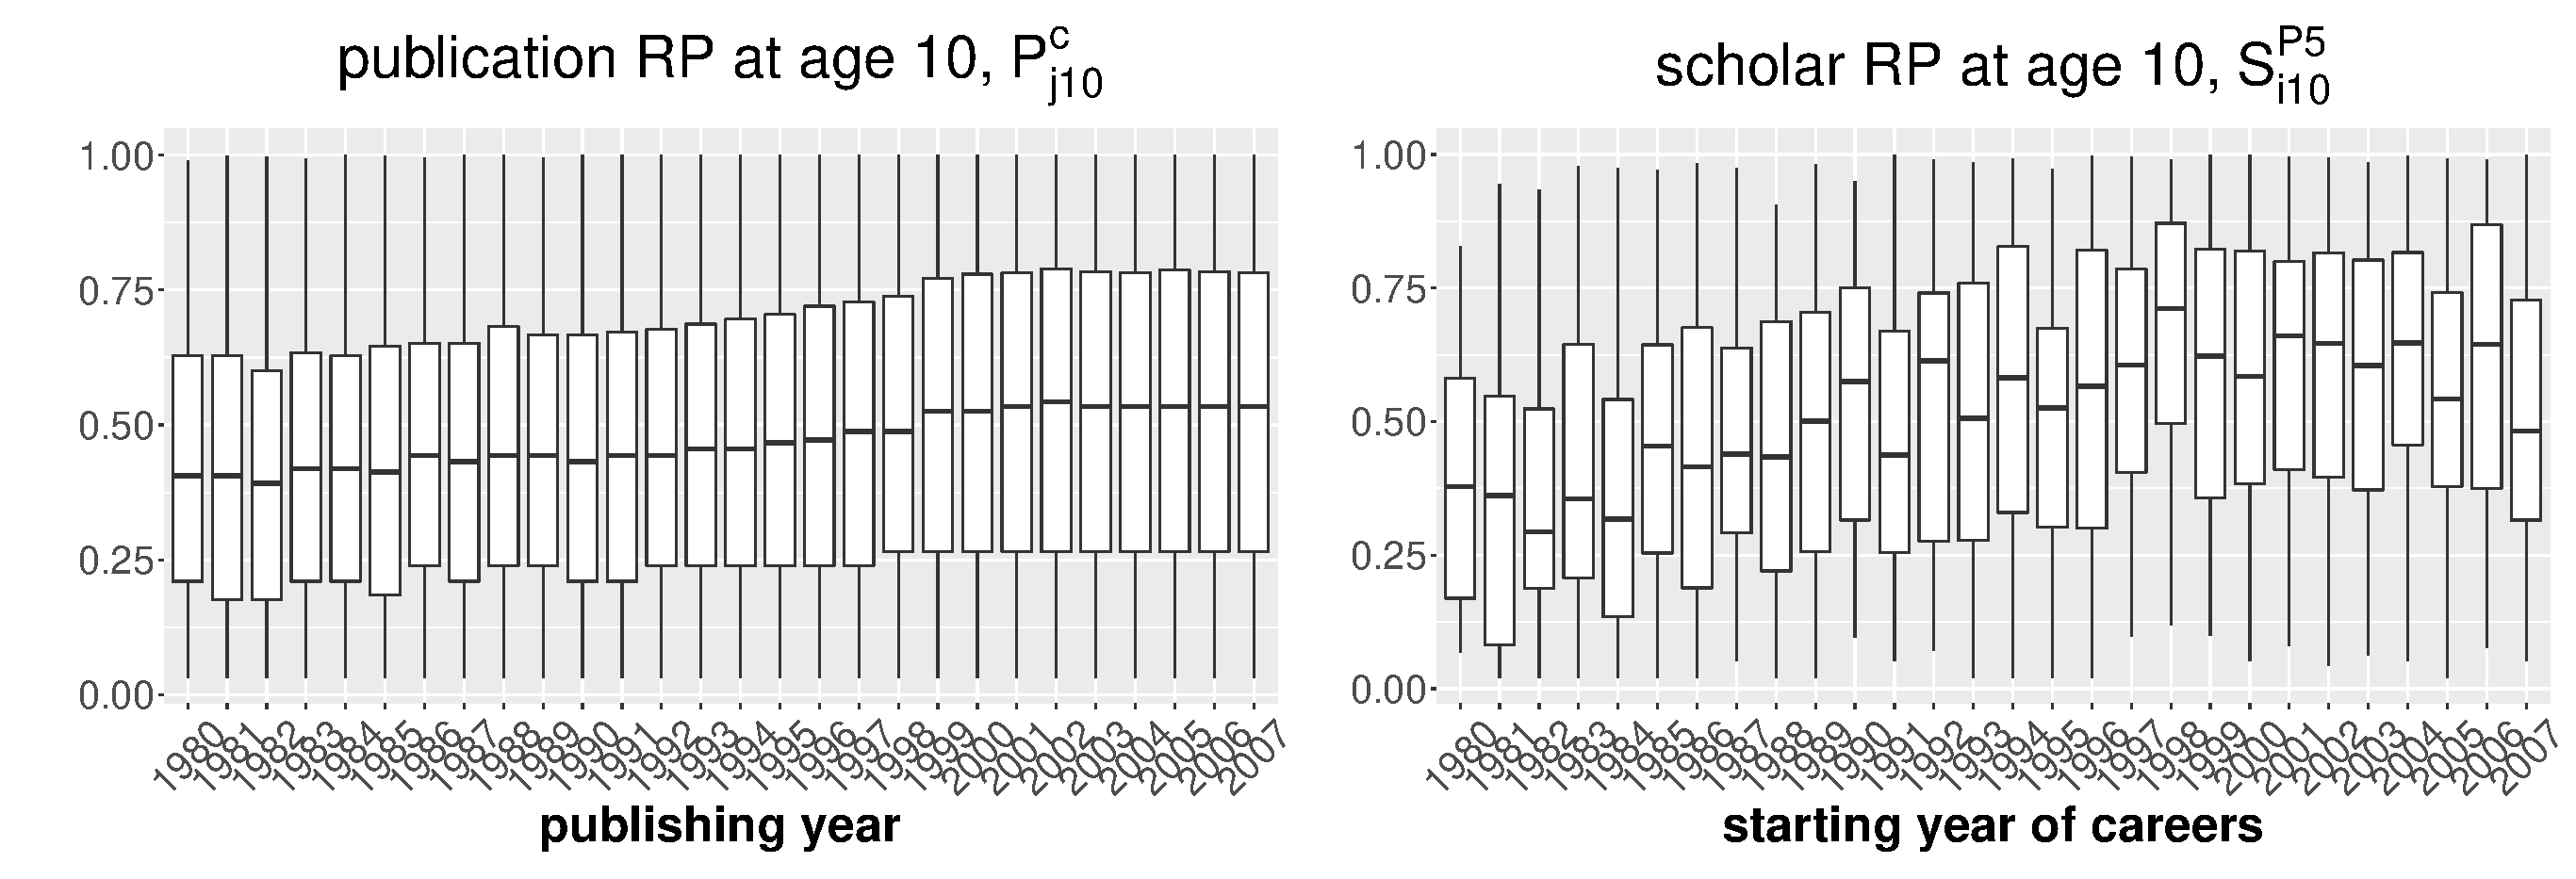
\includegraphics[width=\textwidth]{figures/exploratory/stationarity.eps}
    \caption{P$_{j10}^c$ grouped by the publishing years and and S$_{i10}^{P5}$ grouped by the starting years of academic careers. The benchmark contains professors from various disciplines who receive their tenureships no later than year $2016$.}
    \label{fig:stableness_rp}
\end{figure}

\subsection*{The predictability of the rank percentile indicators}
% publication rank percentile vs citations, predictability, Wang(2013)
\begin{figure}[ht!]
     \centering
     \begin{subfigure}[b]{0.48\textwidth}
         \centering
         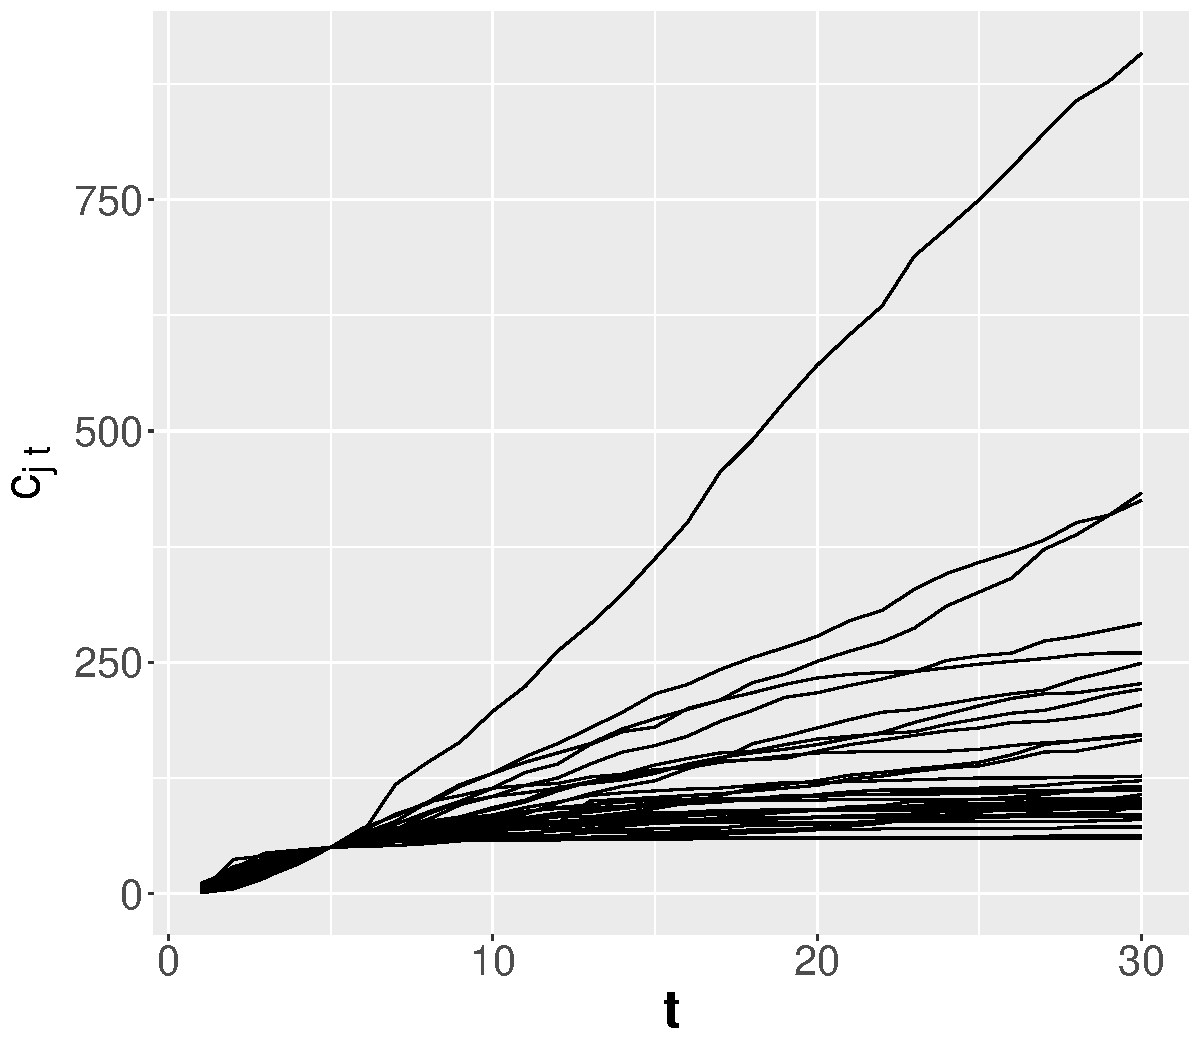
\includegraphics[width=\textwidth]{figures/pred_power/ncit_vs_pubrp/cit_age.pdf}
         \caption{}
         \label{fig:pred_cit_age}
     \end{subfigure}
     \hfill
     \begin{subfigure}[b]{0.48\textwidth}
         \centering
         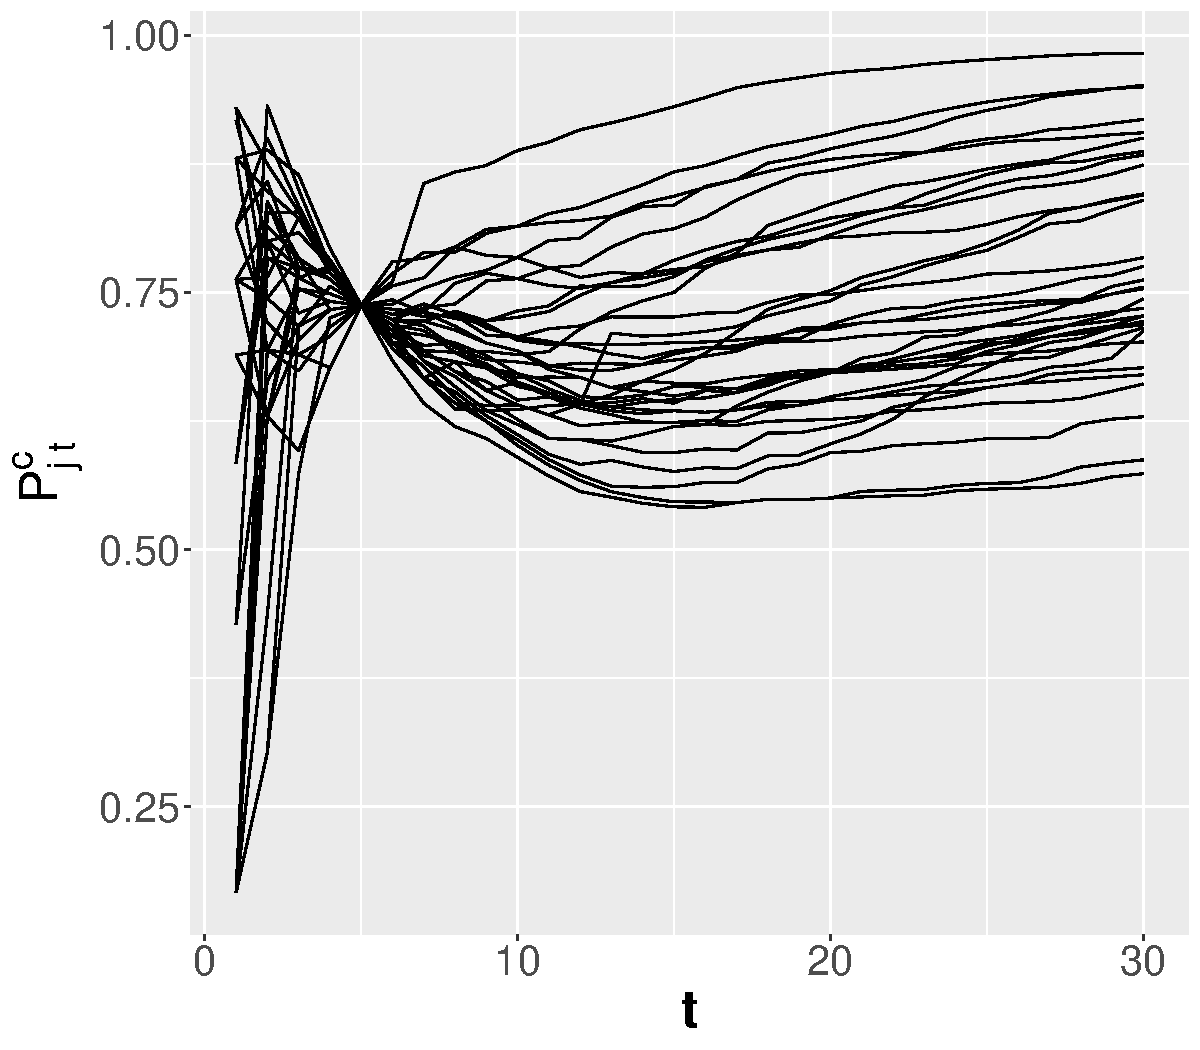
\includegraphics[width=\textwidth]{figures/pred_power/ncit_vs_pubrp/rp_age.pdf}
         \caption{}
         \label{fig:pred_rp_age}
     \end{subfigure}
     \hfill
     \begin{subfigure}[b]{0.48\textwidth}
         \centering
         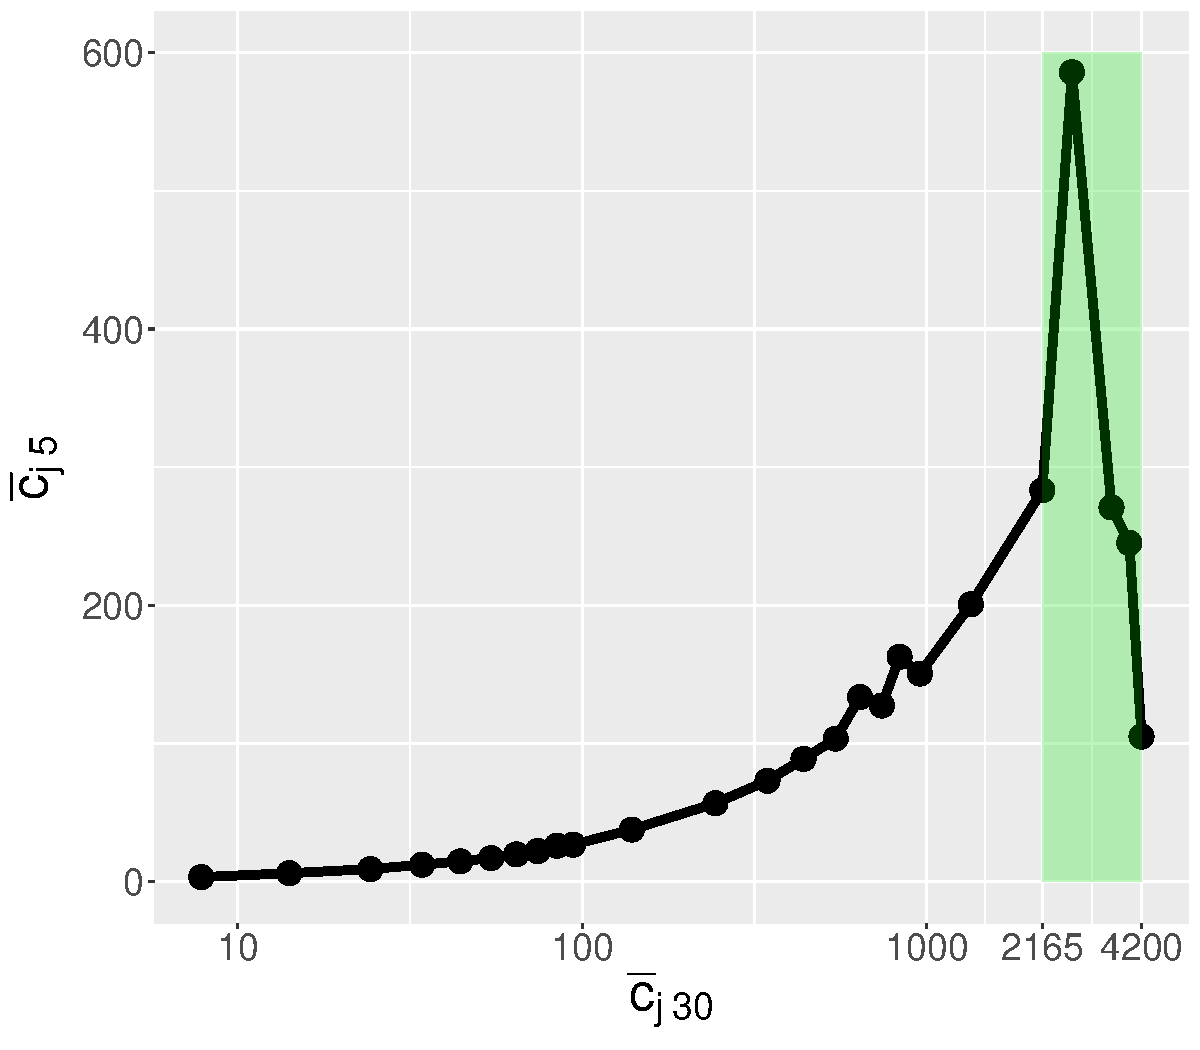
\includegraphics[width=\textwidth]{figures/pred_power/ncit_vs_pubrp/cit_cit.pdf}
         \caption{}
         \label{fig:pred_cit_cit}
     \end{subfigure}
     \hfill
     \begin{subfigure}[b]{0.48\textwidth}
         \centering
         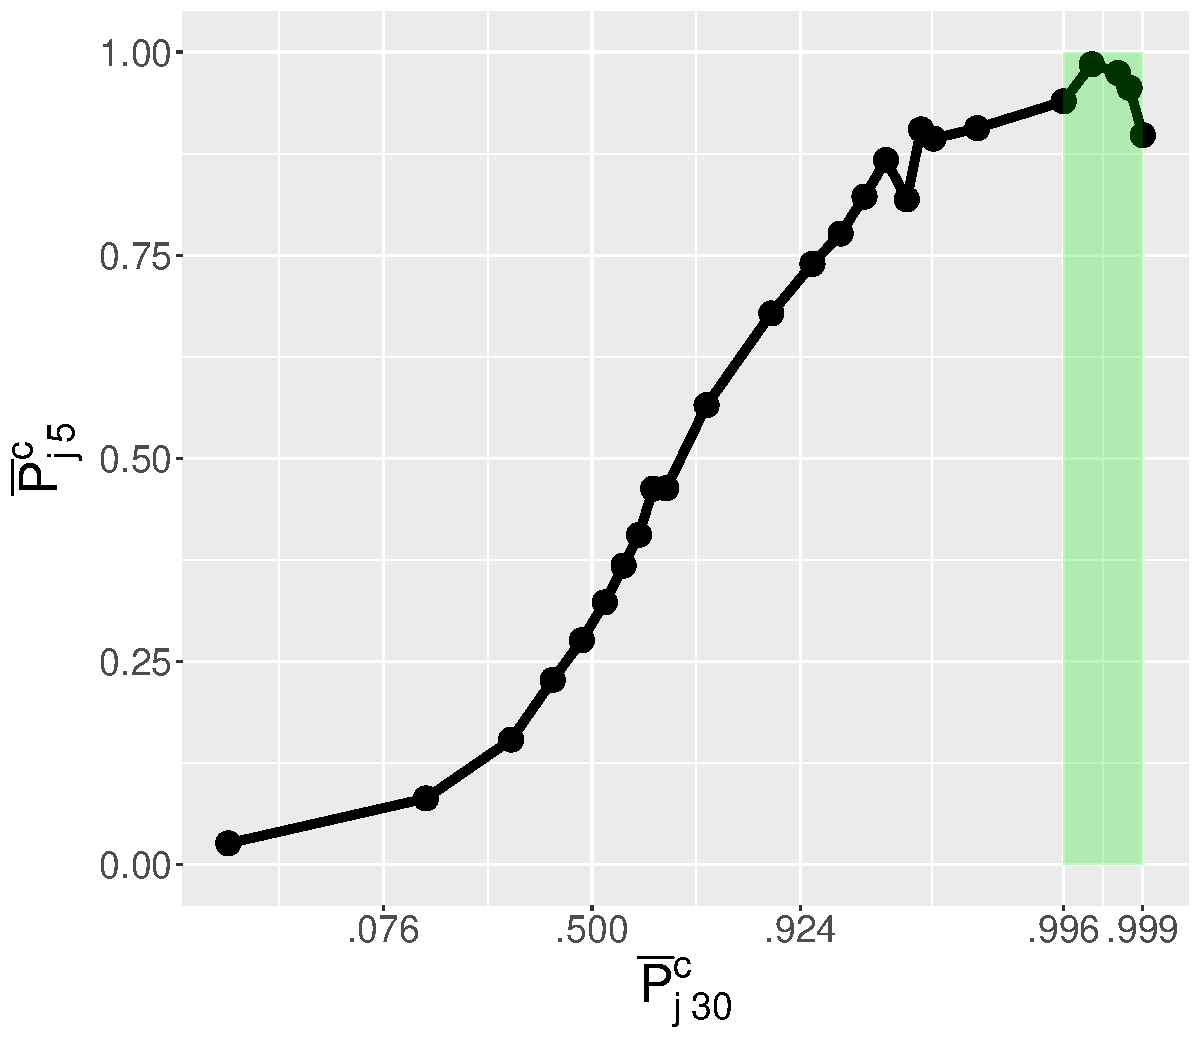
\includegraphics[width=\textwidth]{figures/pred_power/ncit_vs_pubrp/rp_rp.pdf}
         \caption{}
         \label{fig:pred_rp_rp}
     \end{subfigure}
        \caption{The predictability of citations and rank percentiles. The benchmark here is biology. Figure \ref{fig:pred_cit_age} and \ref{fig:pred_rp_age} show the citations and the corresponding rank percentiles for papers that have $50$ citations by age $5$. Figure \ref{fig:pred_cit_cit} displays the average citations by age $5$ over the average citations by age $30$, for different sets of publications, which are pre-specified by dividing the range of $\bar{c}_{j 30}$ into equal intervals in the log scale. Figure \ref{fig:pred_rp_rp} shows the corresponding average rank percentiles for the same sets of publications. Note that we do not claim originality for these plots, as figures \ref{fig:pred_cit_age} and \ref{fig:pred_cit_cit} have been illustrated via a different dataset\supercite{Wang2013}.}
        \label{fig:pub_cit_rp_pred}
\end{figure}


% publication rank percentile, heat map of correlations
\begin{figure}[ht!]
    \centering
    \begin{subfigure}[b]{0.8\textwidth}
        \centering
             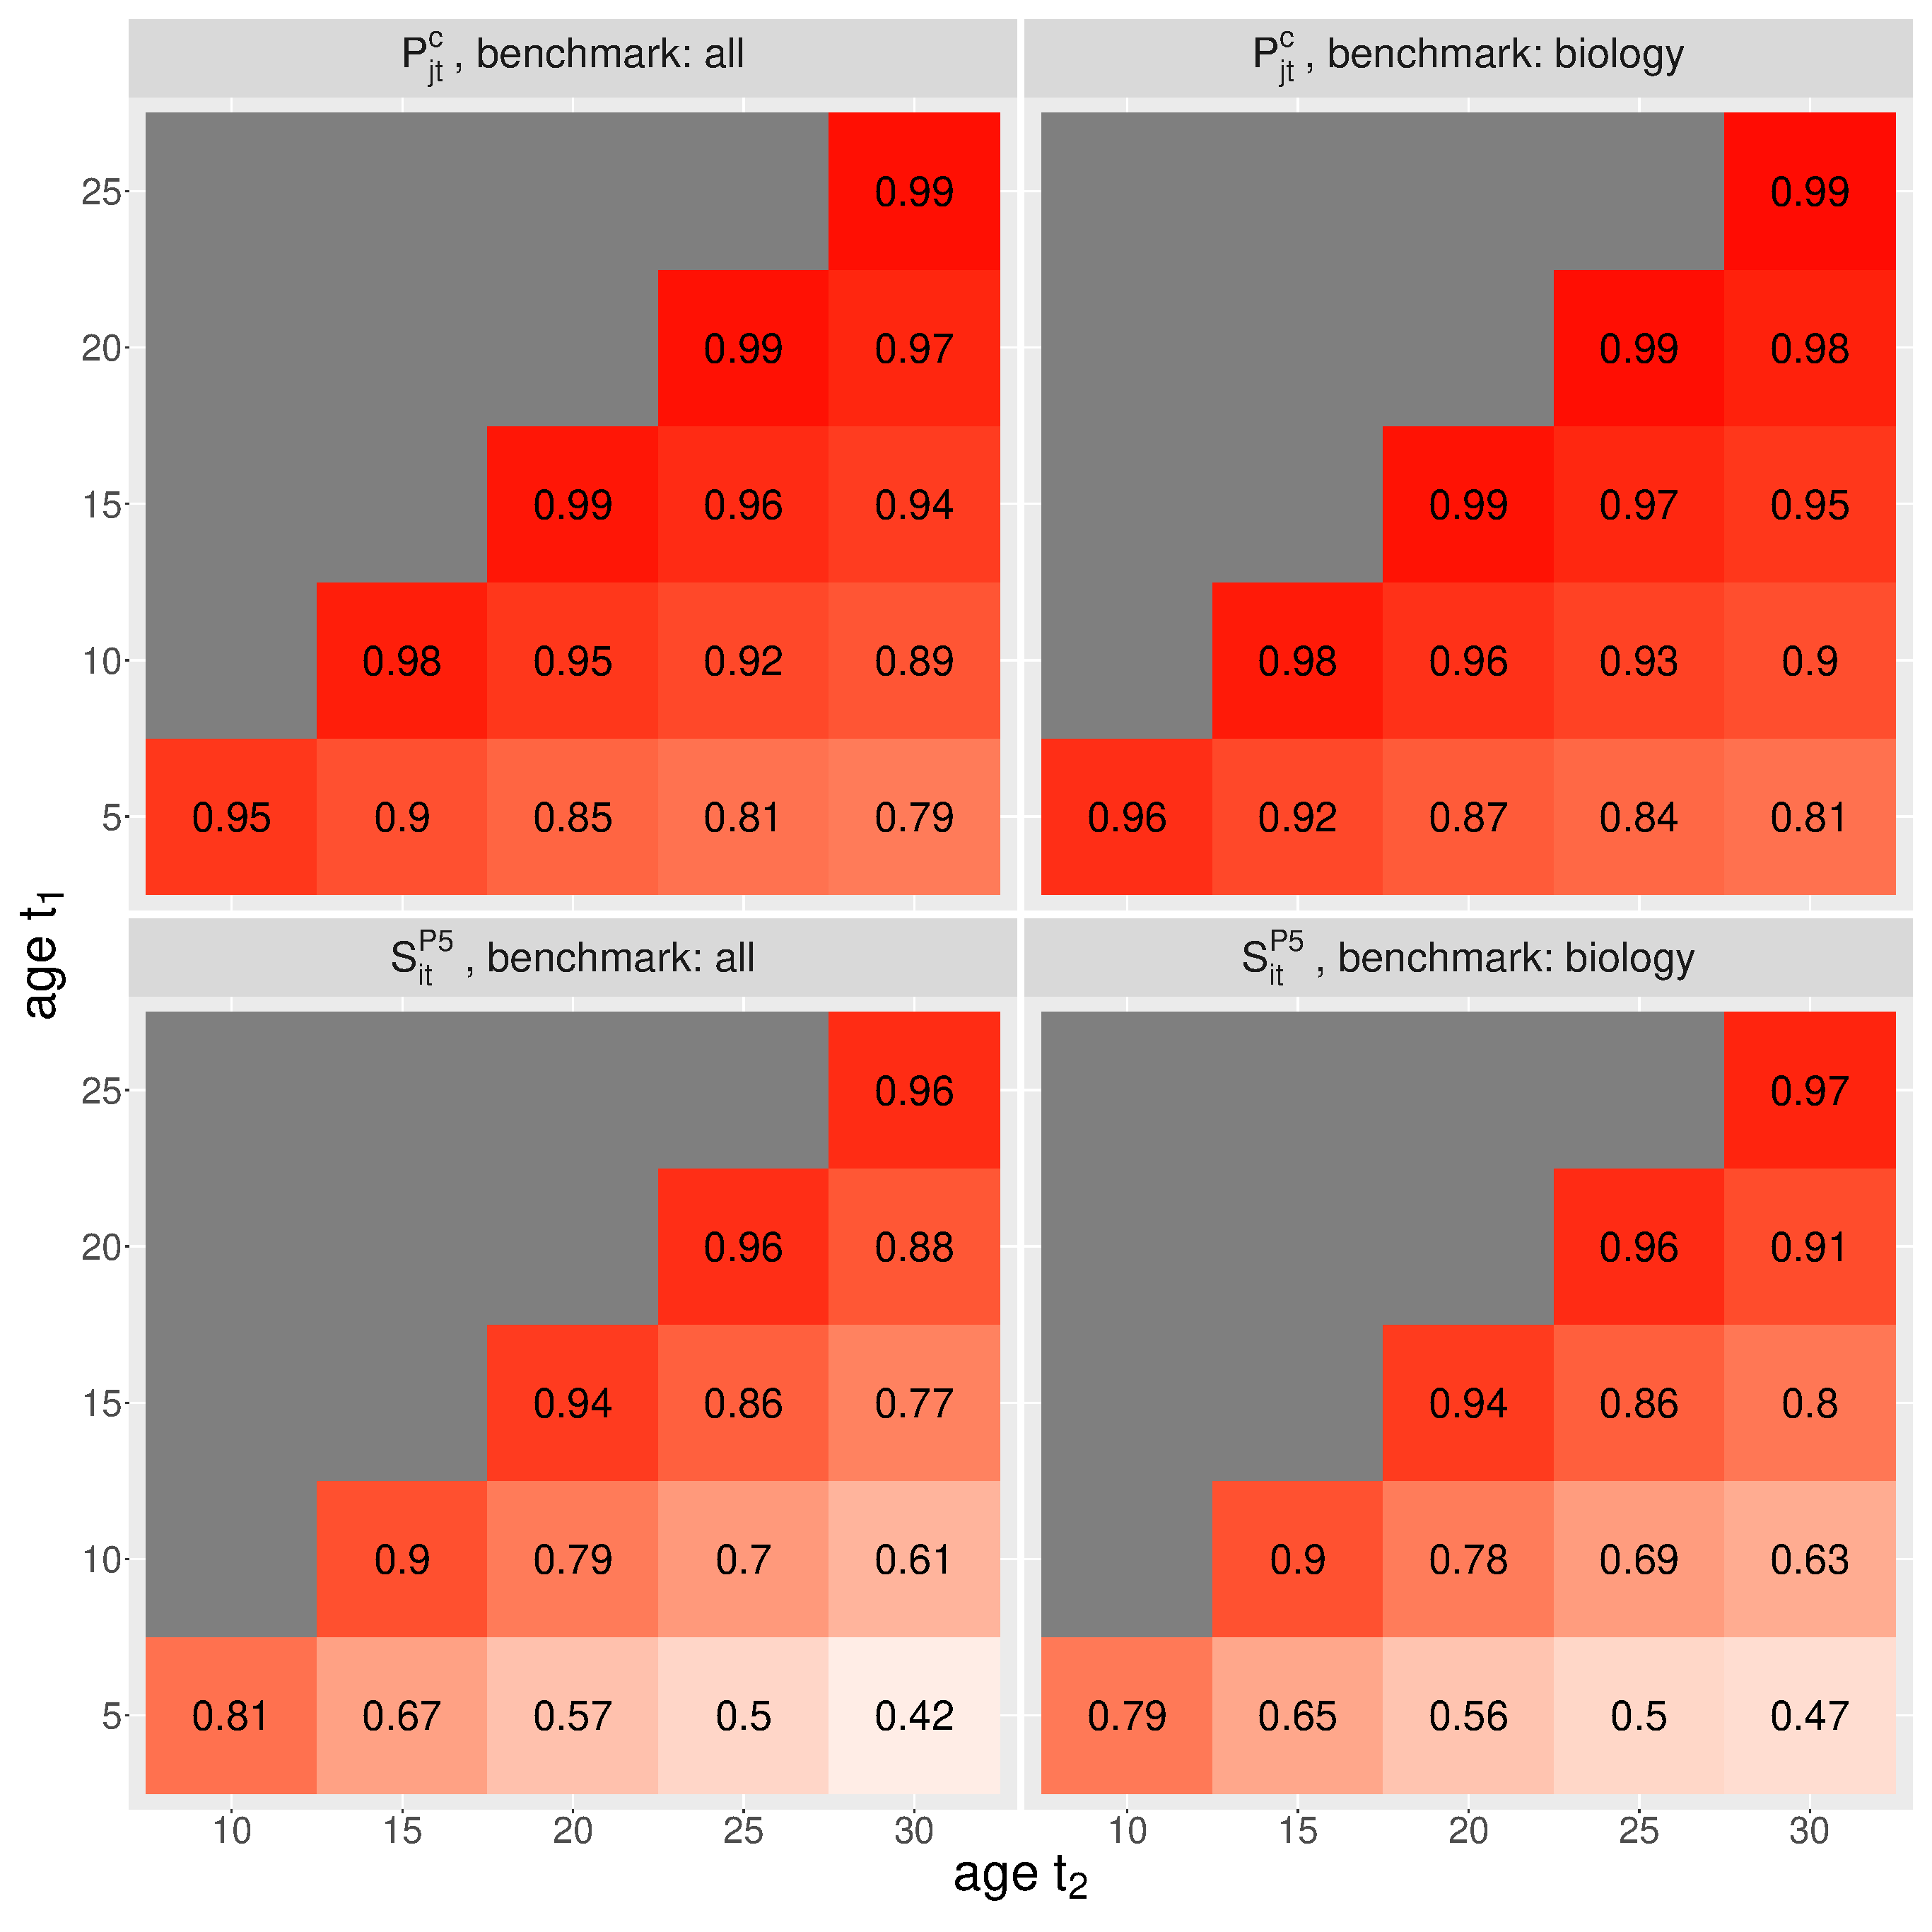
\includegraphics[width=\textwidth]{figures/pred_power/current/heatmap_cor.eps}
         \caption{Predict the cumulative impacts}
         \label{fig:hm_rp_current}
    \end{subfigure}
    
    \begin{subfigure}[b]{0.8\textwidth}
        \centering
             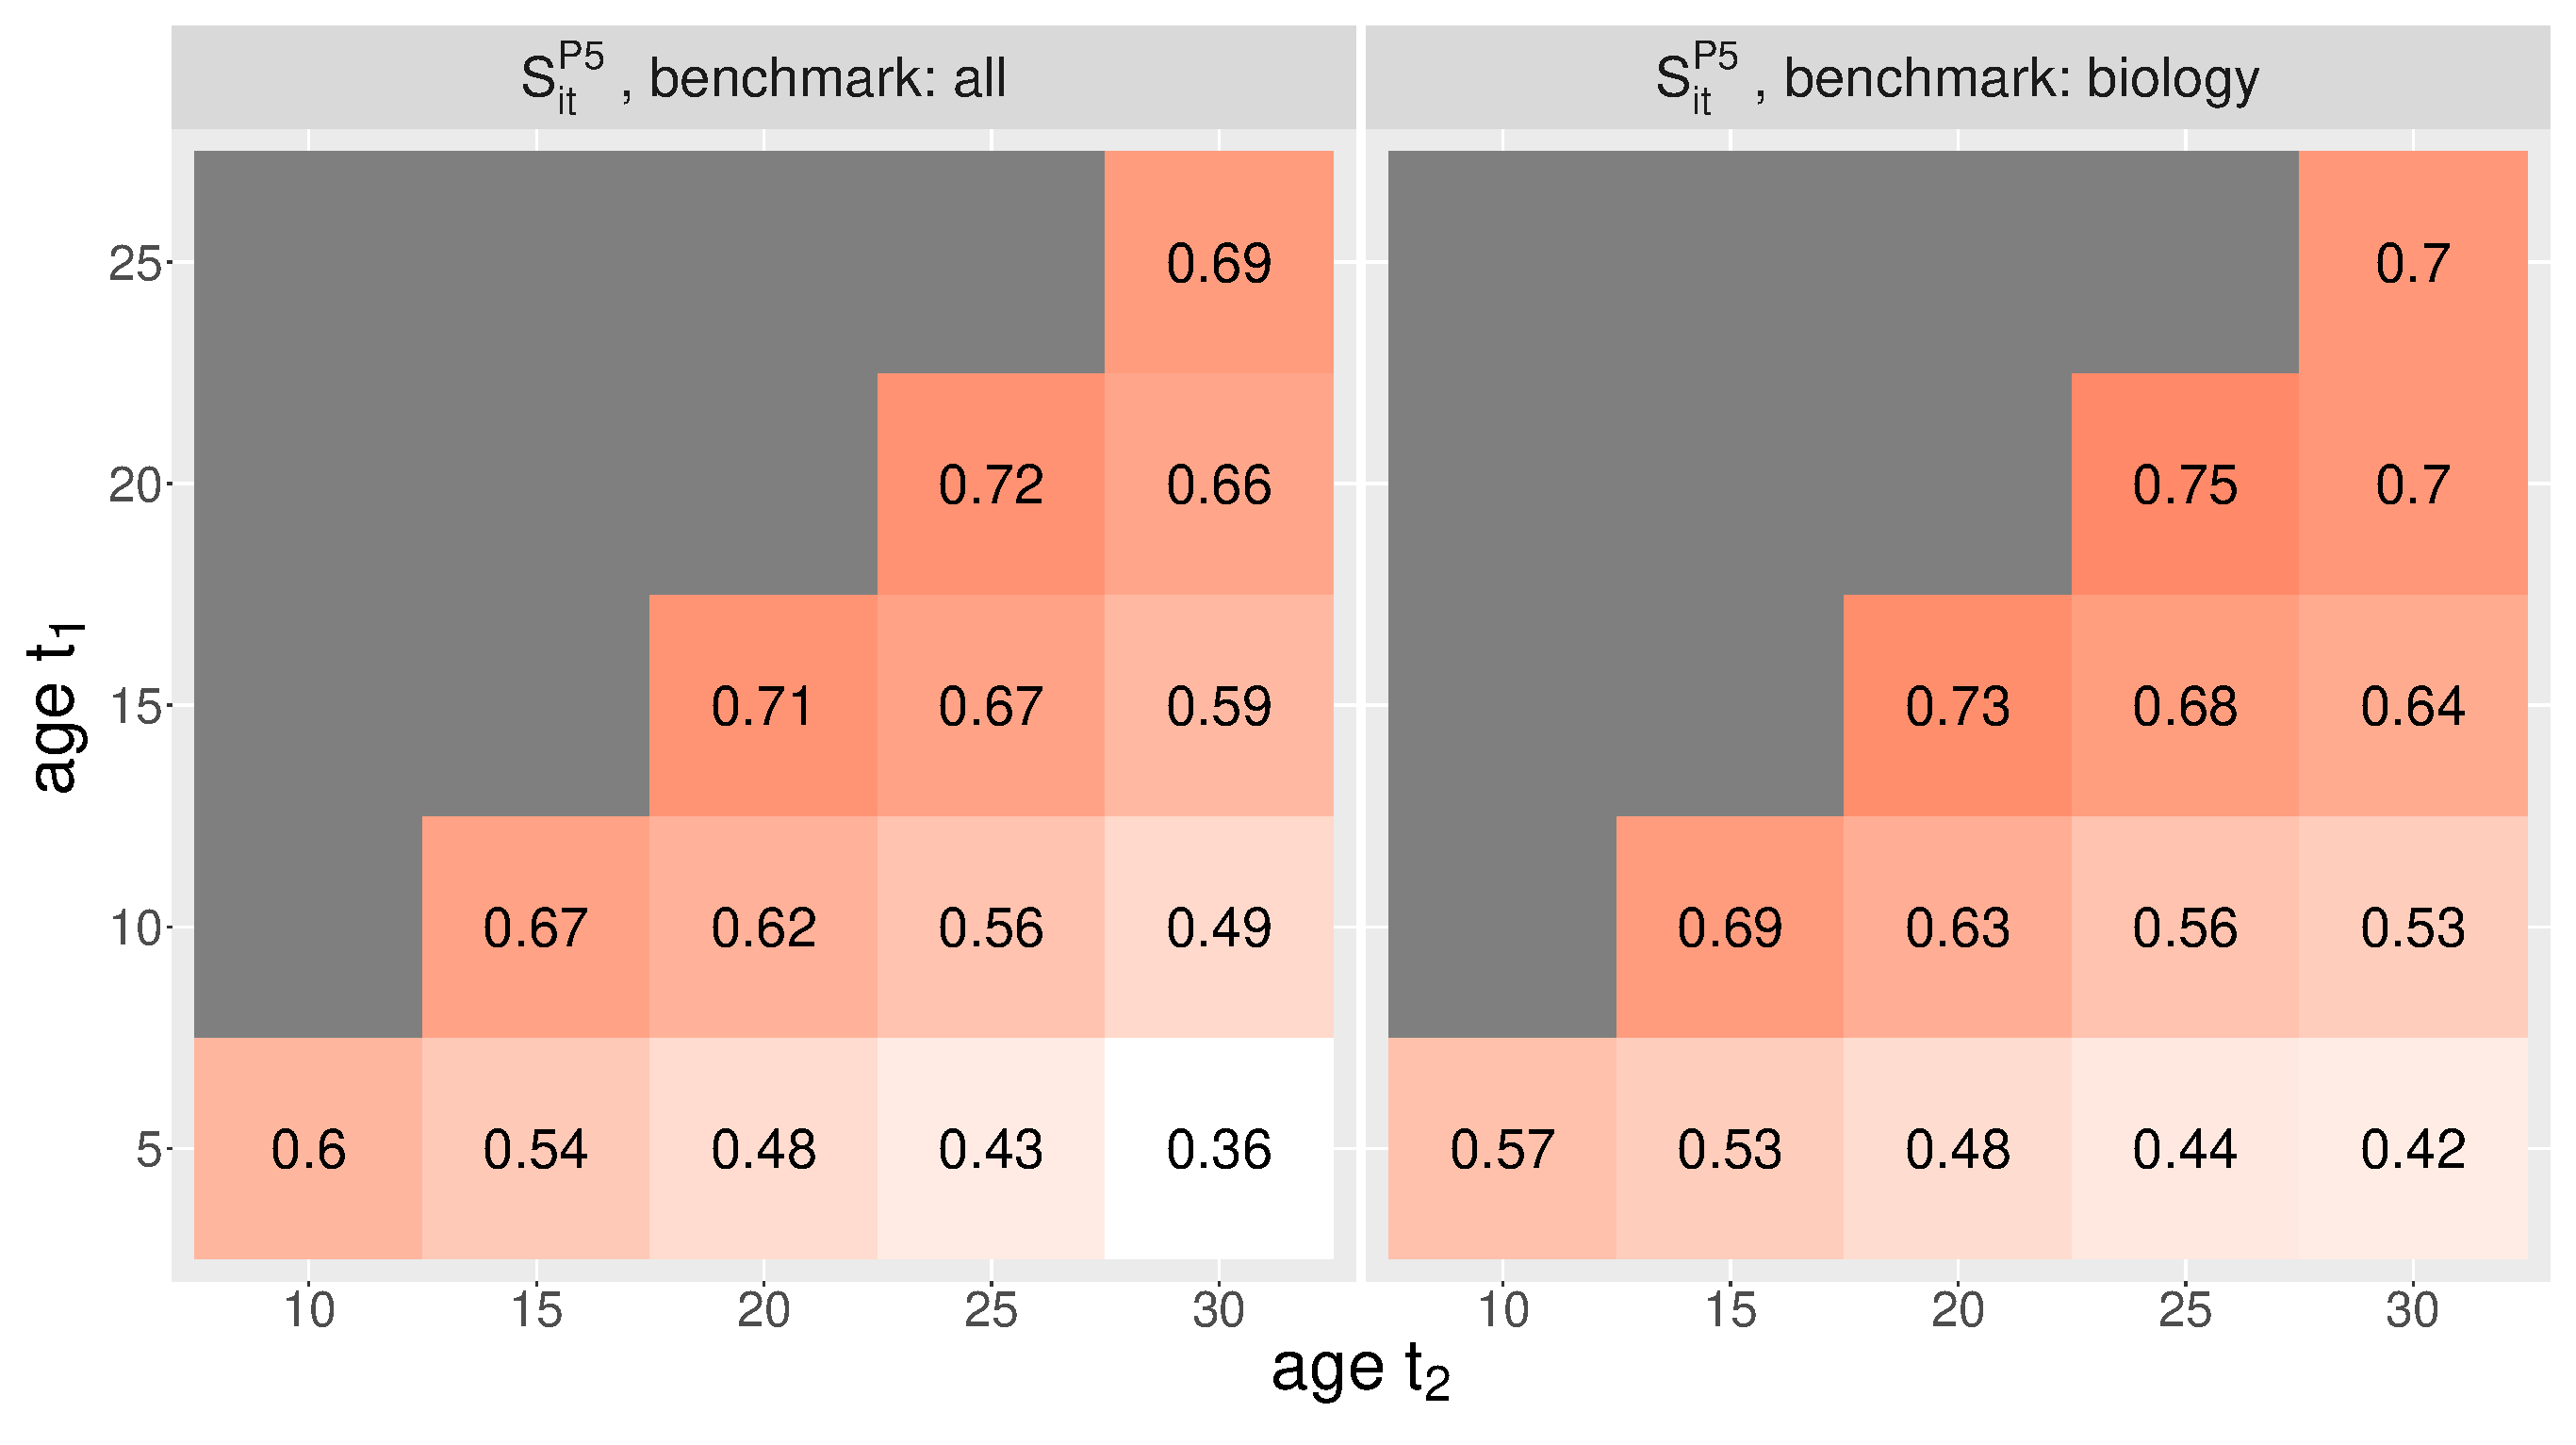
\includegraphics[width=\textwidth]{figures/pred_power/future/heatmap_cor.eps}
         \caption{Predict the future scientific output}
         \label{fig:hm_rp_future}
    \end{subfigure}
    \caption{The Pearson's correlation between RP indicators at two different ages. }
    \label{fig:hm_rp}
\end{figure}
\begin{figure}[ht!]
    \centering
    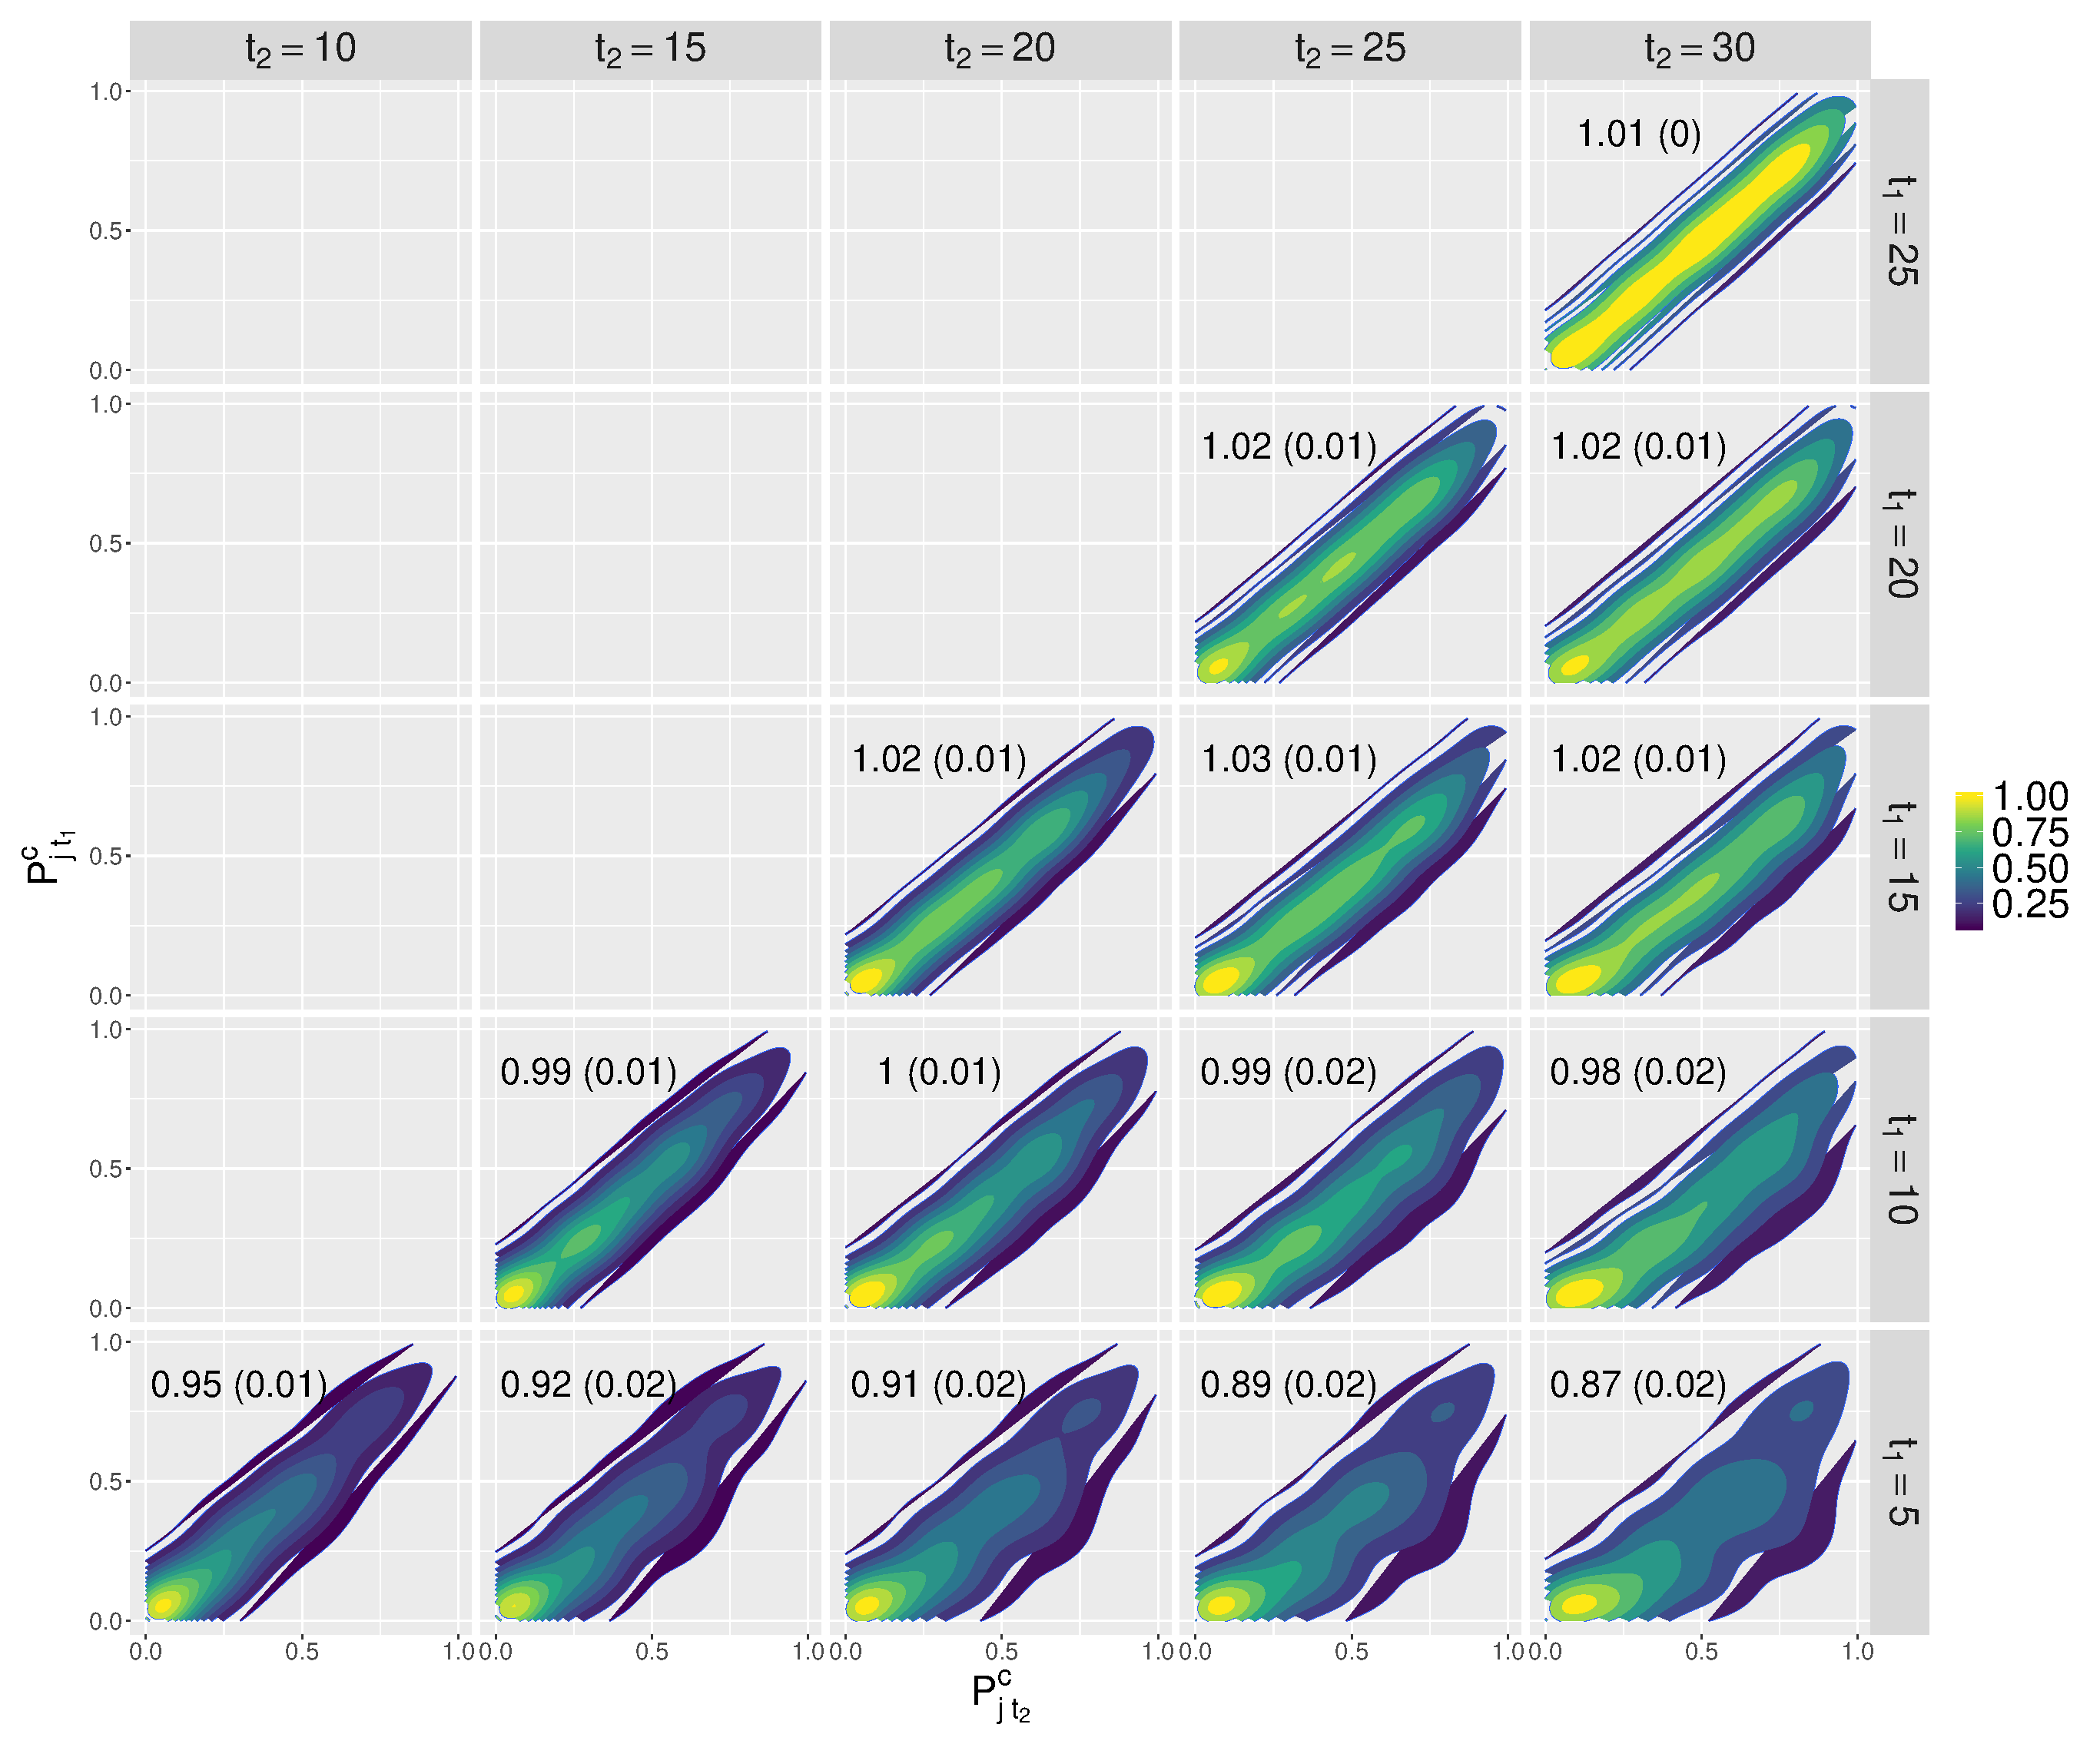
\includegraphics[width=\textwidth]{figures/pred_power/pubrp/scatter_bio1980.eps}
    \caption{Kernel density estimation of the scatters of P$_{j t_1}^c$ and P$_{j t_2}^c$. Meanwhile, we fit a simple linear regression of P$_{j t_2}^c$ upon P$_{j t_1}^c$. The estimated coefficient and the corresponding standard error (in the bracket) are displayed in each facet. The benchmark here includes all publications in biology and written in $1980$.}
    \label{fig:scatter_pubrp_bio1980}
\end{figure}


\begin{figure}[ht!]
    \centering
    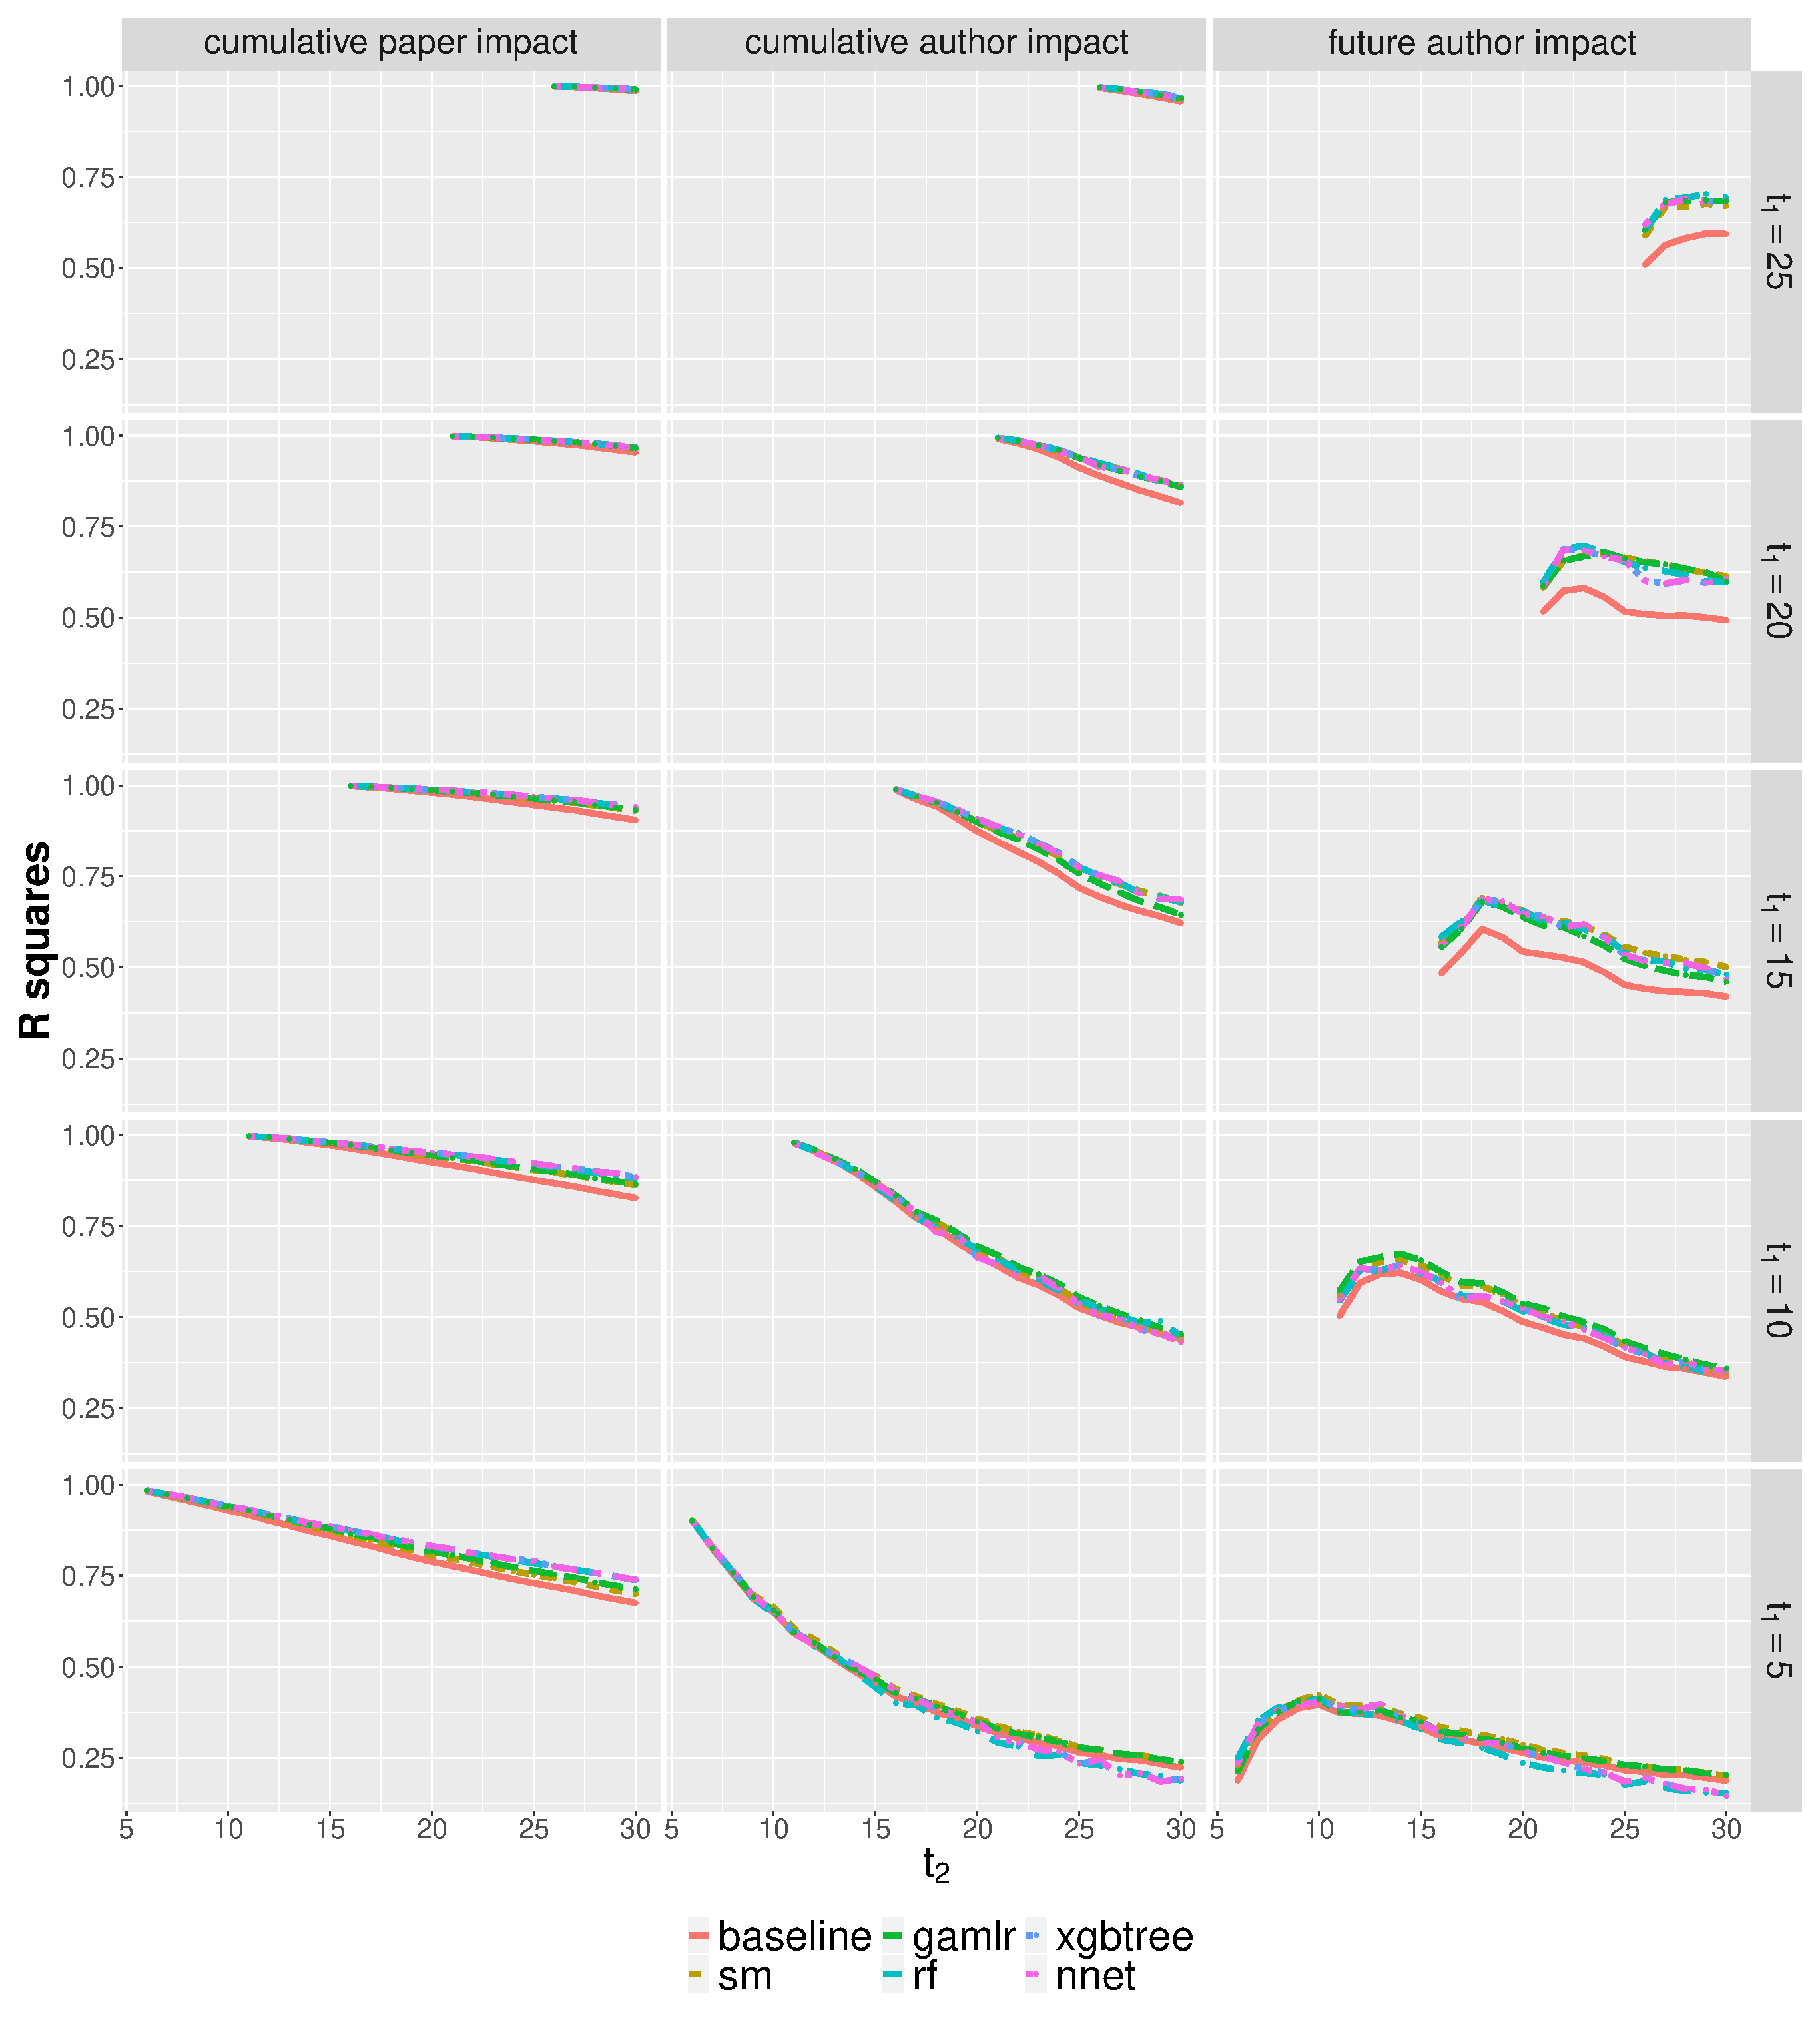
\includegraphics[width=\textwidth]{figures/pred_model/r2_diff.eps}
    \caption{Testing R squares of the predictive models. LASSO, ridge and elastic net are outperformed by Gamma LASSO, and hence are ignored for a better visualization.}
    \label{fig:pred_r2}
\end{figure}


\subsection*{A discussion on various types of rank percentile indicators for scholars}
S$_{it}^{c,b}$, S$_{it}^{h,b}$ and S$_{it}^{P5,b}$ are built upon an aggregation of the performances of the papers that the scholar publish by age $\tau$. S$_{it}^{c,b}$ and S$_{it}^{h,b}$ use the citations $c_{jt}$ to evaluate publication $j$ while S$_{it}^{P5,b}$ uses P$_{j5}^{c,b}$, i.e. the rank percentile of publication $j$ at age $5$. Meanwhile, the aggregation function for S$_{it}^{c,b}$ and S$_{it}^{P5,b}$ is sum, and it's a threshold function for S$_{it}^{h,b}$. 

S$_{it}^{P5,b}$ improves the major drawbacks of the other two indicators. First, it removes the seniority effect of publications, by evaluating the publications by their performances at age $5$. However, both the citations c$_{it}$ and h-index h$_{it}$ are dominated by 'senior' publications and newly published works can hardly contribute. Second, it improves over S$_{it}^{c,b}$ since it hardly rewards authors who publish a large number of low-impact works or only participate in a small number of high-impact projects. Similar to the h-index, the evaluation metric m$_{it}$ of rp.rp5 limits the contribution of a single publication to be at most $1$ due to the definition of rank percentile. However, the absolute number of citations is unlimited and is highly influenced by extreme values. Last, by comparing with rp.h, it penalizes authors who are not truly innovative, but carefully massage their h-indices by publishing a number of papers that are not top-class but attract just enough amount of citations to boost the h-index. As long as a paper is among the top h papers, the actual number of citations is irrelevant for rp.h, but it still affects rp.rp5.

We demonstrate these advantages of rp.rp5 by examining some extreme cases. We create three synthetic academic careers. Author A publishes a substantial number of publications at each age (more than $90\%$ of other authors in the benchmark), while all of the publications have little impacts. Meanwhile, author B and author C only publish $1$ paper at the beginning of their careers, where author B's paper is astonishing while author C's is average. All three authors have h-index as $1$ throughout their careers. Figure \ref{fig:simulated_authors} shows the author rp for these three artificial authors. We see that for author A and B, rp.c is substantially larger than the other two, and it dies down slowly. Even though author B only publishes one ground-breaking paper, the author remains in the top $50\%$ even by age $12$. Both rp.rp5 and rp.h are better characterizing the performances of these authors. Meanwhile, author C has the same rp.h as author B although his/her publication has much less impact. In this case, rp.rp5 and rp.c are better especially at the beginning of the careers. 

Besides these special cases, for the majority of authors in our dataset, we see a large agreement between rp.rp5 and the other two types of rp. Consider the benchmark being biology. In order to study the agreement, for each indicator, we classify the authors into four classes, class $1$: $0\le \text{rp} < 0.25$, class $2$: $0.25\le \text{rp} < 0.5$, class $3$: $0.5 \le \text{rp} < 0.75$ and class $4$: $0.75 \le \text{rp} \le 1$. An agreement in the classification of an author is where two (or three) different rp belong to the same class. The overall agreement for all three rp is $51\%$ at age $5$ and $68\%$ at age $30$, i.e. about half of the authors result in the same classifications of the three rp at age $5$, while that number becomes around two third at age $30$. Figure \ref{fig:aut_rp_class} shows the detailed classifications for every pair of the three rp. As we can see that, the agreement increases with the age. Furthermore, rp.rp5 has large agreements with both rp.c and rp.h, that are $69\%$ and $67\%$ respectively at age $5$, and $71\%$ and $81\%$ respectively at age $30$. 

We've shown the advantage of using rp.rp5 over indicators like rp.c and rp.h. A remaining question is why we use rp.c$_{j5}$ rather than say rp.c$_{j10}$ to represent the quality of the paper. It turns out that rp.c$_{j\tau}$ is highly stable over ages, and rp.c$_{j5}$ is very close to rp.c$_{j10}$ for the majority of papers. This will be discussed in the section below. Therefore, we are using less citation information and get similar accuracies. Other choices involve taking the summary statistic of the entire history of rp.c$_{j\tau}$ ($\tau=1,\cdots,T_j$). For example, we can take the best performance along the history, i.e. $\displaystyle \max_{t=1,\cdots,T_j} \text{rp.c}_{jt}$. We demonstrate that the evaluation metric m$_{i\tau}$ formulated based on these alternatives is highly correlated with m$_{i\tau}$ formulated rp.c$_{j5}$. Furthermore, the rank percentile indicators based on these alternatives are not statistically different from rp.rp5. The details are discussed in the supplemental material section \ref{sec:robustness_rprp}.

\subsection*{Predictive power of rank percentile indicators}
Citations have been shown to lack long-term predictive power\supercite{Wang2013}. Figure \ref{fig:pred_cit_age} shows that publications with the same citations by age $5$, can have noticeably different citation paths and long-term effects. Meanwhile, exceptional and creative ideas can normally take longer to be appreciated by the community. As shown in figure \ref{fig:pred_cit_cit}, the correlation between short-term citations and long-term citations breaks down for most highly-cited papers (the shaded area). Such problems affect less for rank percentiles, as evidenced by figure \ref{fig:pred_rp_age} and \ref{fig:pred_rp_rp}. For the papers having rp.c$_{j 5} \approx 0.75$, their rp.c$_{j 30}$ are all above $0.5$. Meanwhile, the correlation between short-term and long-term rp is still very strong for the most highly-cited papers. 

Publication rp.c$_{j\tau}$ and scholar rp.rp5$_{i\tau}$ are highly predictive and stable over age. Figure \ref{fig:hm_rp_current} shows the ability of the indicators to predict their own values. We see an extremely high predictive power for rp.c, which indicates that a publication with high rp.c after $\tau_1$ ages is very likely to have high rp.c after $\tau_2$ ages where $\tau_2 > \tau_1$. Meanwhile, the predictive power dies down as the forecast horizon gets larger, which simply reflects the difficulty of long-term forecast. Also, the correlation becomes higher when we have a longer history of the publication, e.g. it increases from $0.79$ to $0.86$ as $\tau_1$ changes from $5$ to $10$ while keeping the forecasting horizon fixed at $\tau_2-\tau_1=5$. Finally, we see a slightly higher predictive power when we restrict the benchmark to only include publications in biology.

Similar patterns can be observed for rp.rp5 according to figure \ref{fig:hm_rp_current}, although it has lower predictive power than rp.c. To be more specific, it starts with a high predictive power but dies down fast as the forecast horizon becomes larger. For instance, the correlation drops from $0.99$ to $0.94$ for rp.c while it decreases from $0.94$ to $0.77$ for rp.rp5, by fixing $\tau_1=15$. This is result from the fact that forecasting future impact of future works is considerably harder than forecasting the future impact of existing works. Predicting rp.c$_{j\tau_2}$ belongs to the latter. On the other hand, rp.rp5$_{i\tau_2}$ is based on the set of papers that scholar $i$ publishes by age $\tau_2$, which contains papers published by $\tau_1$ and papers published in the period of $(\tau_1,\tau_2]$. Hence, predicting rp.rp5$_{i\tau_2}$ involves predicting the future impact of existing works as well as the future impact of future works. As the forecast horizon $\tau_2-\tau_1$ becomes larger, we potentially have more `predicting the future of future' to deal with that makes the task tougher. Meanwhile, other types of scholar rank percentile indicators, rp.c and rp.h, have very similar predictive powers with rp.rp5, which is illustrated in figure \ref{fig:hm_autrp_current}.

It turns out that not only do publication rp.c has high predictive power, it's stable over age, i.e. rp.c$_{j\tau_1}\approx$rp.c$_{j\tau_2}$. Figure \ref{fig:scatter_pubrp_bio1980} shows the kernel densities of the scatters of rp.c$_{j\tau_1}$ vs rp.c$_{j\tau_2}$. We see that the scatters are mostly along the $45$ degree line. Meanwhile, we perform a simple linear regression by regressing rp.c$_{j\tau_2}$ upon rp.c$_{j\tau_1}$. The regression coefficient of variable rp.c$_{j\tau_1}$ together with the standard error is displayed besides each of the scatters in the figure. We see that the coefficients are very close to $1$ with very small standard errors, which gives further evidence that rp.c is stable over age. Meanwhile, figure \ref{fig:scatter_autrp_all} shows a similar study for the stableness of rp.rp5. We do not see strong evidence of rp.rp5 being stable over age.

We know that predicting rp.rp5 involves forecasting the future impact of both existing and future works. Such question can assist making decisions for a faculty position or tenureship, since the committee would like to examine the cumulative scientific impact of the scholar. A more difficult question is to predict the future impact of the future works. Such question is of interest, for example, in assigning research fundings or allocating research resources, where the future impact of existing works shall be irrelevant. Figure \ref{fig:hm_rp_future} shows the ability of using rp.rp5$_{i\tau_1}$ to predict rp.rp5$_{i\tau_2 \setminus \tau_1}$, where the latter is based on only the future papers, i.e. those written in the $(\tau_1,\tau_2]$ time interval. As expected, we see lower a predictive power than predicting rp.rp5$_{i\tau_2}$, but rp.rp5$_{i\tau_1}$ can still explain most of the variations in rp.rp5$_{i\tau_2 \setminus \tau_1}$ in relatively short horizons. 

\subsection*{Predictive models}
For both the publication and scholar impact, we've studied how well the performance by age $\tau_1$ predicts the cumulative achievement by age $\tau_2$. We demonstrate that rank percentile indicators (rp.c$_{j\tau}$ and rp.rp5$_{i\tau}$) have high predictive powers. Meanwhile for the scholar impact, we further investigate the prediction of performance in the subsequent $\tau_2-\tau_1$ ages, i.e. using rp.rp5$_{i\tau_1}$ to predict rp.rp5$_{i\tau_2 \setminus \tau_1}$. 

We now formulate these prediction tasks as supervised learning problems, and examine how much improvement we can get by having an extensive list of features and complex fitting algorithms. We consider the following fitting procedures; these models are ordered by increasing complexity, starting from simple baselines and ending with complex machine learning models:
\begin{itemize}
    \item Baseline: a simple linear regression of rp$_{\star \tau_2}$ upon rp$_{\star \tau_1}$.
    \item Simple Markov model (sm): a linear regression model of rp$_{\star \tau_2}$ upon features only including rp$_{\star \tau_1}$ and the change of rp over the last $2$ ages.
    \item Penalized linear regression models, including ridge\supercite{hoerl1970ridge}, LASSO\supercite{tibshirani1996regression}, elastic net (enet)\supercite{zou2005regularization} and the Gamma LASSO (gamlr)\supercite{taddy2017one}: linear models with different penalties on the regression coefficients. All of these methods shrink the coefficients towards zero, and the later three methods can provide sparse solutions (shrink the coefficients to exactly zeros). 
    \item Ensemble methods of regression trees, including random forest (rf)\supercite{liaw2002classification} and extreme gradient boosting trees (xgbtree)\supercite{chen2016xgboost}: rf is a bagging of regression trees with a subset of randomly selected features chosen at each split to avoid overfitting. xgbtree is a fast implementation of gradient boosting on regression trees with a model formation that emphasizes the role of regularizations to avoid overfitting.
    %\item Support vector regression (svr)\supercite{drucker1997support}: 
    \item Deep neural networks (dnn): feedforward networks with multiple hidden layers and using dropout and $l_2$ regularization to avoid overfitting.
\end{itemize}

\subsubsection*{Features and model fitting}
A crucial step for supervised machine learning models is feature engineering. The features that we create are based on the citation histories and are characterized into either author related or paper related features. For example, to predict the author impact rprp5$_{i\tau_2}$, an author related feature can be the number of papers that the author publish by age $\tau_1$, and a paper related feature can be the average citations of these papers. The $30$ features for predicting the publication impact and the $42$ features for predicting the author impact, are listed in tables \ref{tab:features_pubrp} and \ref{tab:features_autrp} respectively. 

The features are created only using the citation information available by $\tau_1$ and the response is specified at $\tau_2$. With a pair of features and response, all the models are trained and evaluated on the testing set, where the training and testing are randomly split in a 9-1 ratio. We consider $5$ different values of $\tau_1$ representing different stages of a publication or a scholar, that are $\tau_1\in\{5,10,15,20,25\}$, and for each $\tau_1$ we have $\tau_2=\tau_1+1,\cdots,30$, which results in $75$ pairs of $(\tau_1,\tau_2)$ in total. Hence all the models are trained $75$ times independently. Meanwhile, the machine learning models all rely on some hyper-parameters that require careful tuning. We use randomized searching with multiple iterations over a pre-specified parameter space, and the optimal set of hyper-parameters is chosen to minimum the 10-fold cross-validation error.

If we ignore the fact that we are modeling rp.c$_{j\tau}$ and rp.rp5$_{i\tau}$ at fixed time points, and view them as time series. Both series turn out to be non-stationary, based on statistical tests such as the Dicky-Fuller test\supercite{dickey1979distribution} and the KPSS test\supercite{kwiatkowski1992testing}, where the details are discussed in the supplemental material section \ref{sec:stationarity_test}. It's often encouraged to work on stationary series, for example in the autoregressive and moving average models, and a typical practice is to model differenced series. We follow the same logic here, and use the differenced series as the responses, e.g. $\Delta \text{rp.c}_{j\tau_2} = \text{rp.c}_{j\tau_2} - \text{rp.c}_{j\tau_1}$. 

\subsubsection*{Results}
We consider four evaluation metrics for the predictive models, that are the R squares ($R^2$), root mean squared error (RMSE), root median squared error (RMEDSE) and mean absolute error (MAE). The $R^2$ for all the models are shown in figure \ref{fig:pred_r2}, while the rest of the metrics are displayed in figure \ref{fig:pred_rmse}, \ref{fig:pred_medse} and \ref{fig:pred_mae}. We see that the baseline model predicts the cumulative impacts well, and the improvement of using more features and machine learning models have little benefit. Meanwhile, the baseline model can still provide reasonable predictions for the future scholar impact, although the machine learning models can provide better results when $\tau_1$ is relatively large. However, in such scenarios, the simple Markov model performs closely to the machine learning models, and hence the extensive list of features and complex non-linearity have little impact.






 %!TEX root = ms.tex
\section*{Discussion}

Rank percentile indicators compare the performance of a publication or a scholar relative to cohorts in the benchmark. They have the advantage of being interpretable and flexible in the choice of benchmark and evaluation metrics. We illustrate that the publication percentile is highly stable, while the scholar percentile exhibits short-term stability and can be predicted utilizing a simple linear regression model. In practice, the highly predictable rank percentiles can be utilized in combination with other metrics to picture the trajectory of a scholar or a publication and assist in academic decision making. 

%!TEX root = main.tex
\section*{Methods}
\noindent\textbf{Data description}
We focus on authors from all fields in the top universities across the States, who have a Google Scholar account by the end of year $2016$. The dataset includes the entire citation history for each publication of these authors. This gives us $14668$ authors in total, and together they contribute to more than $1.3$ million publications that receive around $100$ million citations in total. We've used the benchmark `biology' throughout our discussion. A scholar and all her corresponding publications are flagged as being in the field of biology, if the areas of interests that she lists on Google Scholar contain any of the keywords: `biology', `genetic', `neuroscience' and `cell'. An exploratory description of the dataset is shown in figure \ref{fig:exploratory}. 

\noindent\textbf{Training the machine learning methods}
All the methods are trained in \textit{R}\supercite{RCT2019} with the help of the package \textit{mlr}\supercite{Bischl2016}, which provides a pipeline of training, validating and testing the model. LASSO, ridge, elastic net, random forest and xgbtree are inbuilt learners of the package. Gamma LASSO and deep neural network are trained using packages \textit{gamlr}\supercite{taddy2017one} and \textit{keras}\supercite{Allaire2019} respectively.

All of the machine learning methods require the tuning of hyper-parameters. The process involves deciding the searching space of parameters and evaluating the sets of parameters using the validation data. The optimal model is the one that minimizes the validation error. Table \ref{tab:hyperpara} shows the hyper-parameter(s) for each machine learning model considered in this paper. It's worth noticing that the parameter space can be huge for method like xgbtree where we have an extensive list of tunable parameters. Randomized search with multiple iterations shall be preferred over the grid search in such scenario. Another choice can be using the Bayesian optimization that searches over the parameter space based on the performance gain. Meanwhile, parallel computing can further reduce the computing time.

The data and code are publicly available at \url{https://github.com/sentian/impact-ranking}. 








%\include{metrics}
%\include{pdmodel}
%\include{varmodel}
% %!TEX root = main.tex
\section*{Results}
\subsection*{Fundamental elements of formulating rank percentile indicators}
Four fundamental elements to calculate the rank percentile indicators are (1) entity; (2) benchmark; (3) metric; and (4) age. The entity specifies the target of interest. For example, it can be a publication (P) or a scholar (S). The benchmark (b) characterizes the individuals that the entity is compared against. For instance, the benchmark can be all the publications in computer science. It can also be the faculty members in a department competing for tenure decisions. The metric (m) specifies the way that the entity is evaluated. For example, it can be the number of citations or h-index. Finally, the age (t) is the number of years that the entity has been alive. The age of a publication is the number of years since it was published, while the age of a scholar is the number of years since his/her first paper was published. By combining these four elements, we use P$_{jt}^{m}(b)$ and S$_{it}^{m}(b)$ to denote the rank percentile indicators for publication $j$ and scholar $i$, respectively. 

\subsection*{The framework of calculating rank percentile indicators}
Suppose the benchmark b contains $N$ publications across $T$ years. For each publication $j\in\{1,\cdots,N\}$, we have a history of some evaluation metric m$_{jt}$ (m$_{jt} \ge 0$) at each age $t=1,\cdots,T_j$ where $T_j$ denotes the total number of years since it's published. The rank percentile indicator of publication $j$ at age $t^\star$, P$_{jt^\star}^{m}(b)$, is computed as follows:
\begin{enumerate}[label=(\arabic*)]
    \item Consider all the $N_{t^\star}$ publications that have $T_j \ge t^\star$, and calculate the rank r$_{jt^\star}$ of publication $j$ based on its metric m$_{jt^\star}$. An average rank is assigned to $r_{jt^\star}$ if there exist other publications that have the same metric value as m$_{jt^\star}$. 
    \item The rank percentile is given by
        \begin{equation}
        \label{eq:rp_rank}
            \text{P}_{j t^\star}^{m}(b) = 
                \begin{cases} 
                    0, & \mbox{if } \text{m}_{j t^\star}=0, \\ 
                    (\text{r}_{j t^\star}-0.5)/N_{t^\star}, & \mbox{otherwise}.
                \end{cases}
        \end{equation}
\end{enumerate}
With the compromise $0.5/N_{t^\star}$ in \eqref{eq:rp_rank}, the median paper will be assigned $50\%$ percentile, and the tails of the citation distribution are treated symmetrically\supercite{allen1914storage}.

The above framework can be easily adapted to compute the rank percentile indicators for scholar $i$ at age $t^\star$, S$_{jt^\star}^{m}(b)$. Furthermore, it is flexible in terms of the choice of the evaluation metric and benchmark. In this paper, we study two benchmarks. The first contains all the scholars in our dataset that come from various disciplines, different institutes and have different starting points of careers. The second benchmark only includes scholars in the area of biological science. Meanwhile, we consider two common choices of the evaluation metric, that are the number of citations (c) and h-index (h). The following are the indicators considered in this paper.
\begin{itemize}
    \item rank percentile indicator for publication $j$:
    \begin{itemize}
        \item \textbf{P$_{jt}^c(b)$}: $m_{jt}$ is the total citations $c_{jt}$ that the paper receives by age $t$,
    \end{itemize}
    \item rank percentile indicator for scholar $i$:
    \begin{itemize}
        \item \textbf{S$_{it}^c(b)$}: $m_{it}$ is the total citations $c_{it}$ that the scholar receives by age $t$.
        \item \textbf{S$_{it}^h(b)$}: $m_{it}$ is the h-index $h_{it}$ of the scholar at age $t$.
        \item \textbf{S$_{it}^{P5}(b)$}: $m_{it} = \sum_{j=1}^{N_t^{(i)}} \text{P}_{j5}^c(b)$, where $N_t^{(i)}$ denotes the total number of papers that the scholar publishes by age $t$. For paper with ages less than $5$, i.e. $T_j<5$, we take the most recent performance P$_{jT_j}^c(b)$ instead. 
    \end{itemize}
\end{itemize}

The rank percentile indicators are highly interpretable. For instance, P$_{jt}^c(b)=0.9$, immediately tells us that paper $j$ performs better than $90 \%$ of the papers in the benchmark at age $t$. Furthermore, two papers from different benchmarks, such as different fields, are directly comparable using the rank percentile indicators. 

\subsection*{The stableness of the rank percentile indicators}
The benchmarks that we study in this paper do not restrict the publications to have the same publishing year or the scholars to have the same starting year of their careers. In many situations, we would like to examine a scholar's performance relative to cohorts that are more senior to her. For instance, to make a promotion decision about a candidate who is in the sixth year of her academic career, the committee may compare her with all other faculty members of the department in the sixth year of their academic careers. The comparison will not be valid, if the candidate is more likely to attract citations than her senior colleagues who start their careers many years before. It may well be the academic environment that results in a better performance of the candidate, rather than the internal factors such as the creativity and productivity. 

Figure \ref{fig:stableness_rp} shows P$_{j 10}^c$ grouped by the publishing years and S$_{i 10}^{P5}$ grouped by the starting year of academic careers, where the benchmark contains all the tenured scholars in our dataset. We see that both indicators are reasonably stable over the physical years. We do not see the pattern that papers or scholars attract more citations than those years before, supporting the validity of rank percentile indicators.

\begin{figure}[ht!]
    \centering
    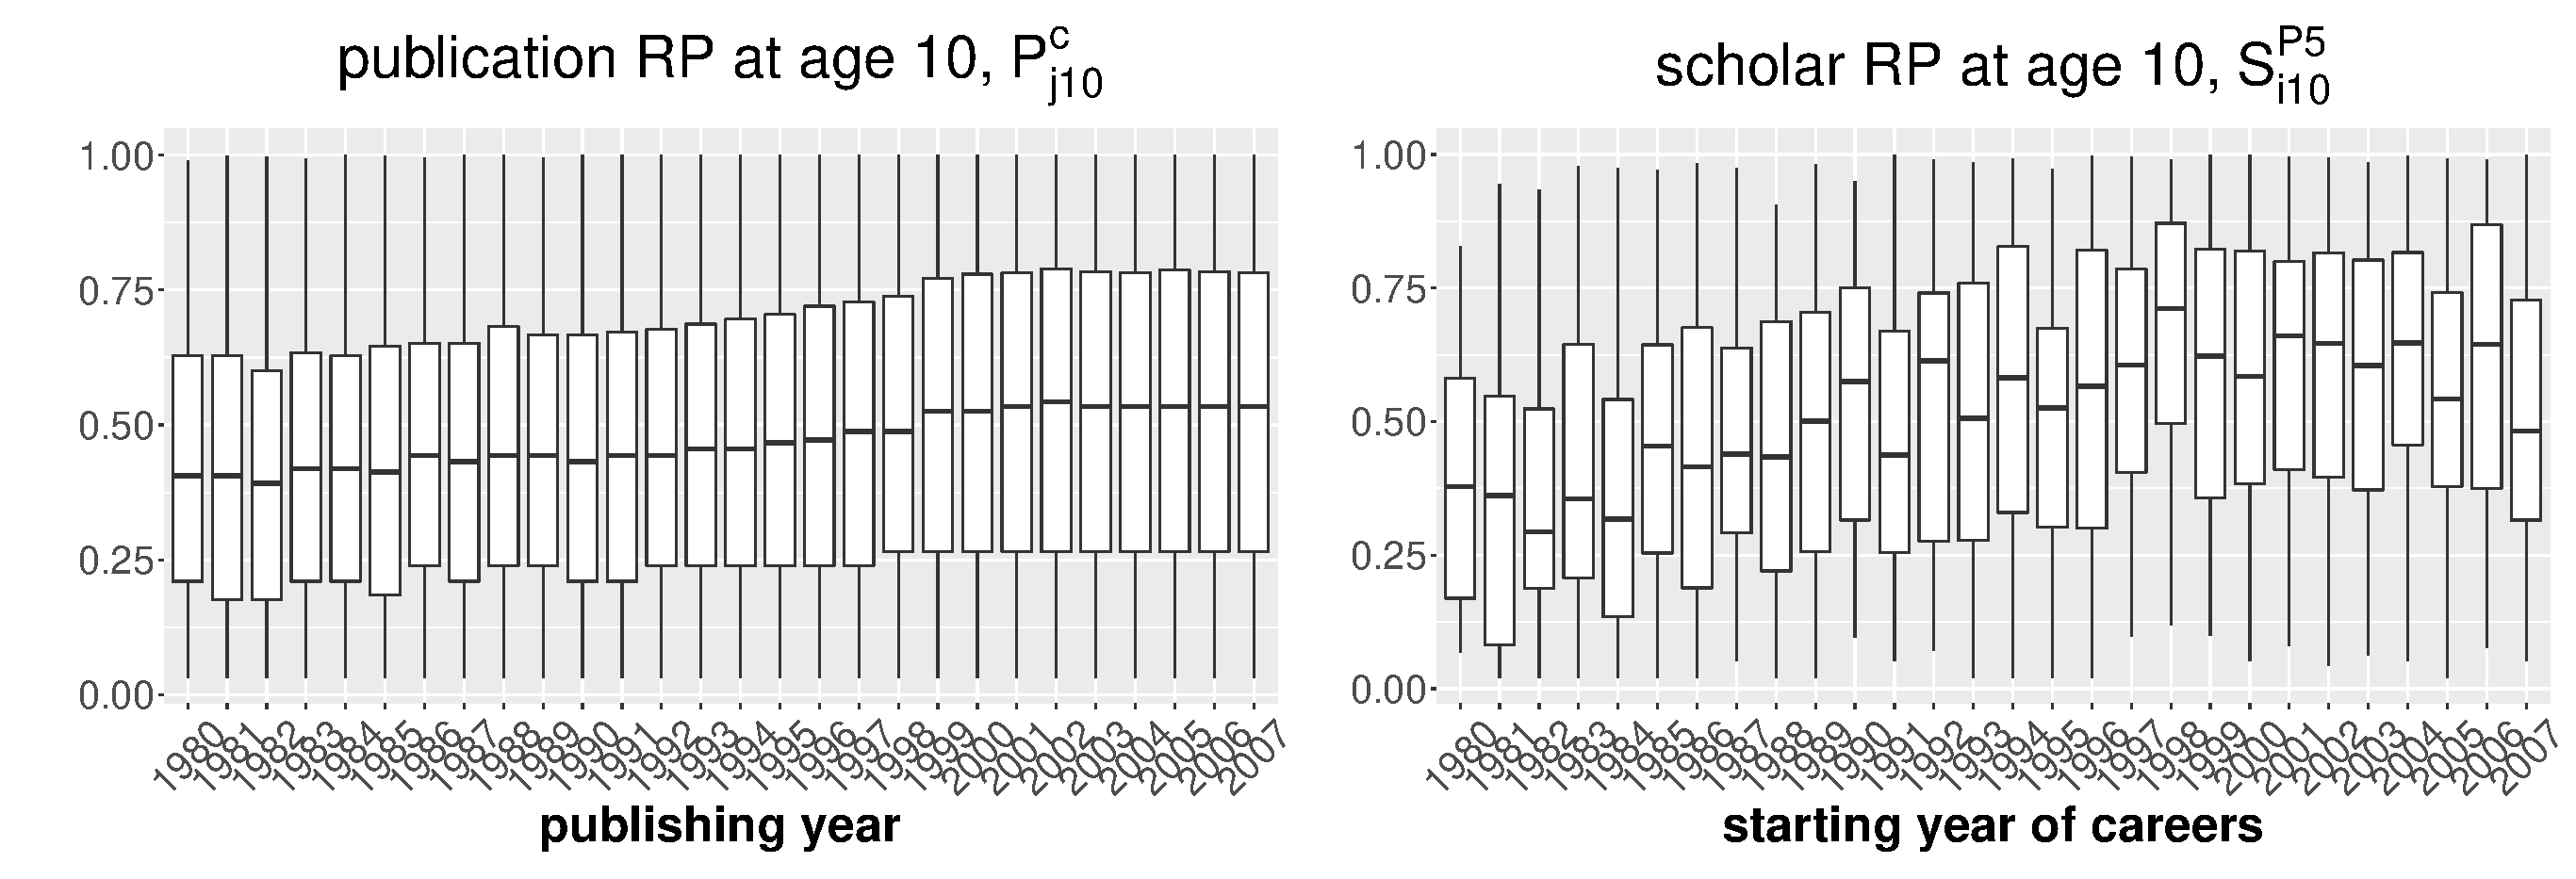
\includegraphics[width=\textwidth]{figures/exploratory/stationarity.eps}
    \caption{P$_{j10}^c$ grouped by the publishing years and and S$_{i10}^{P5}$ grouped by the starting years of academic careers. The benchmark contains professors from various disciplines who receive their tenureships no later than year $2016$.}
    \label{fig:stableness_rp}
\end{figure}

\subsection*{The predictability of the rank percentile indicators}
% publication rank percentile vs citations, predictability, Wang(2013)
\begin{figure}[ht!]
     \centering
     \begin{subfigure}[b]{0.48\textwidth}
         \centering
         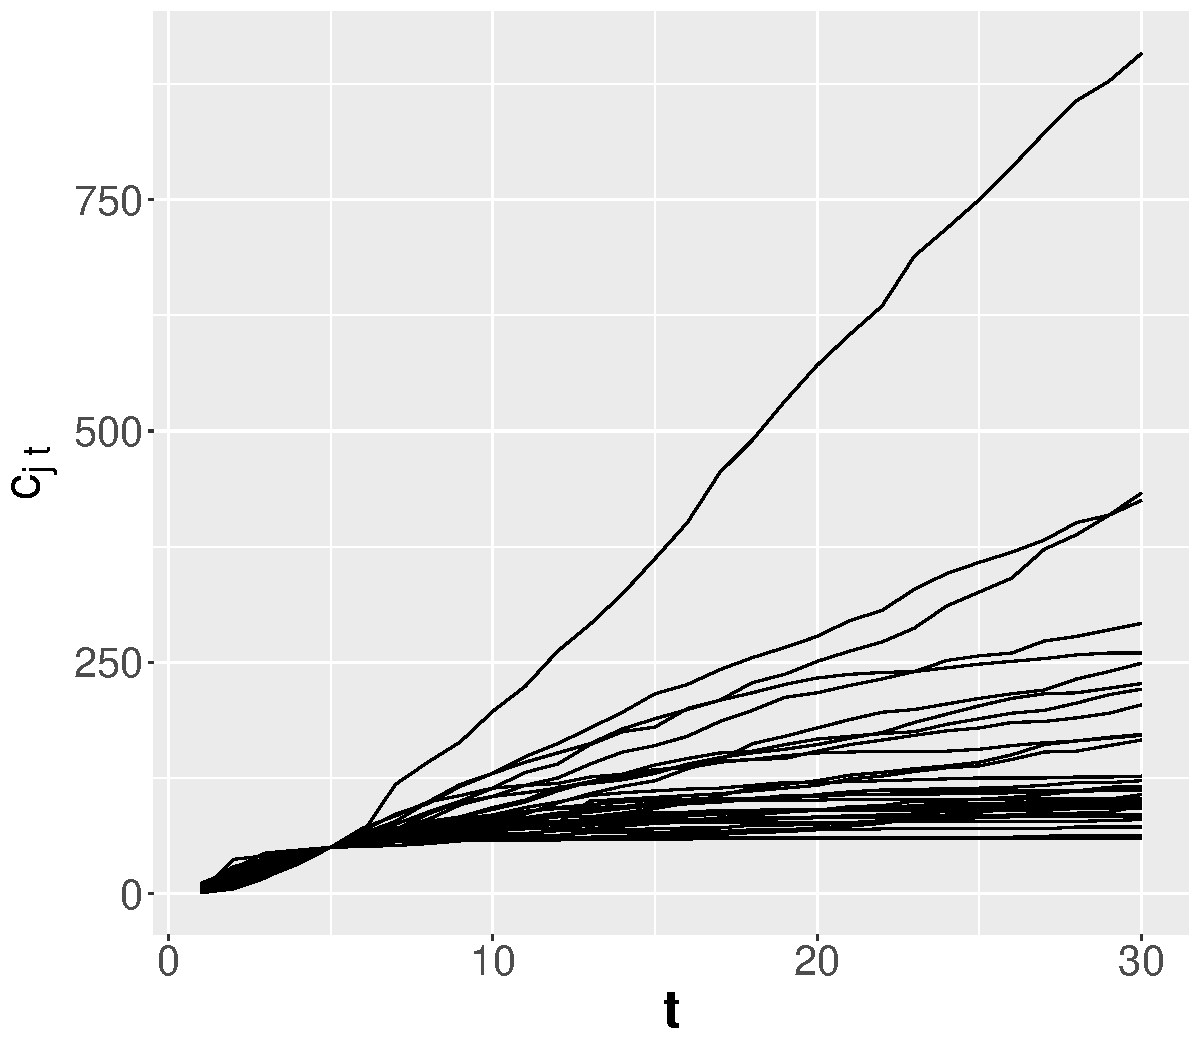
\includegraphics[width=\textwidth]{figures/pred_power/ncit_vs_pubrp/cit_age.pdf}
         \caption{}
         \label{fig:pred_cit_age}
     \end{subfigure}
     \hfill
     \begin{subfigure}[b]{0.48\textwidth}
         \centering
         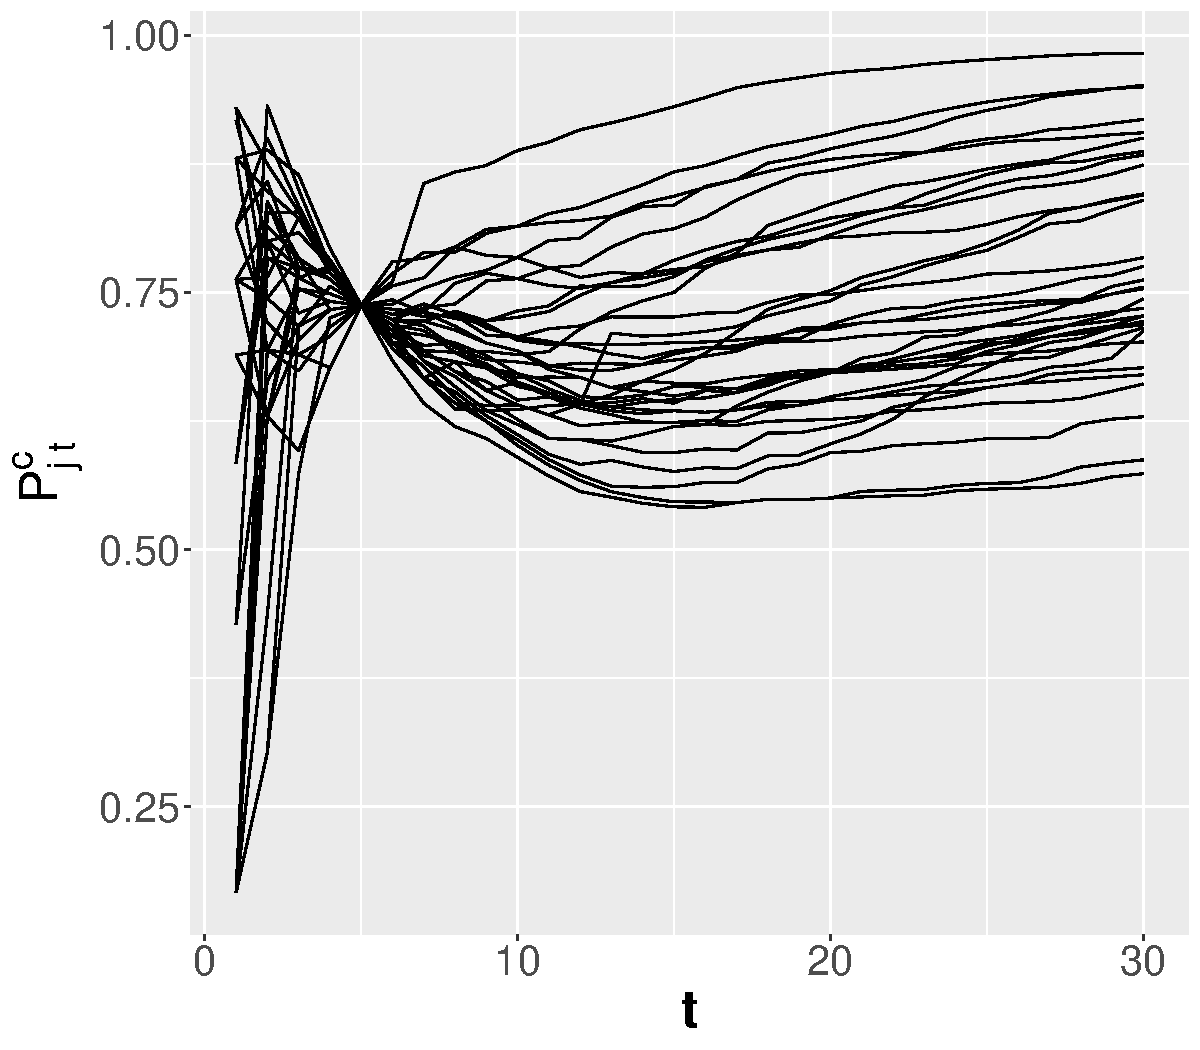
\includegraphics[width=\textwidth]{figures/pred_power/ncit_vs_pubrp/rp_age.pdf}
         \caption{}
         \label{fig:pred_rp_age}
     \end{subfigure}
     \hfill
     \begin{subfigure}[b]{0.48\textwidth}
         \centering
         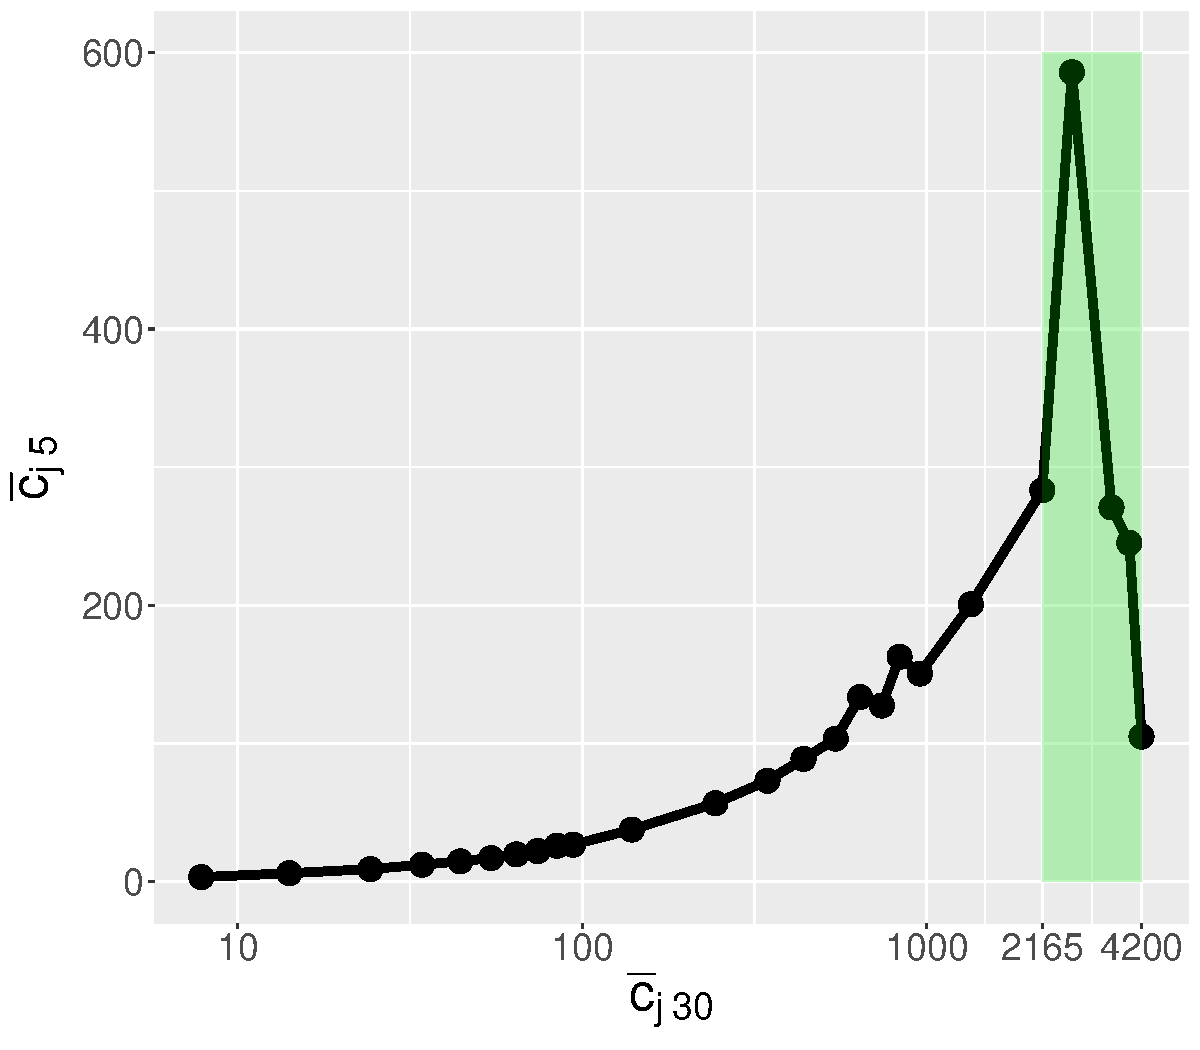
\includegraphics[width=\textwidth]{figures/pred_power/ncit_vs_pubrp/cit_cit.pdf}
         \caption{}
         \label{fig:pred_cit_cit}
     \end{subfigure}
     \hfill
     \begin{subfigure}[b]{0.48\textwidth}
         \centering
         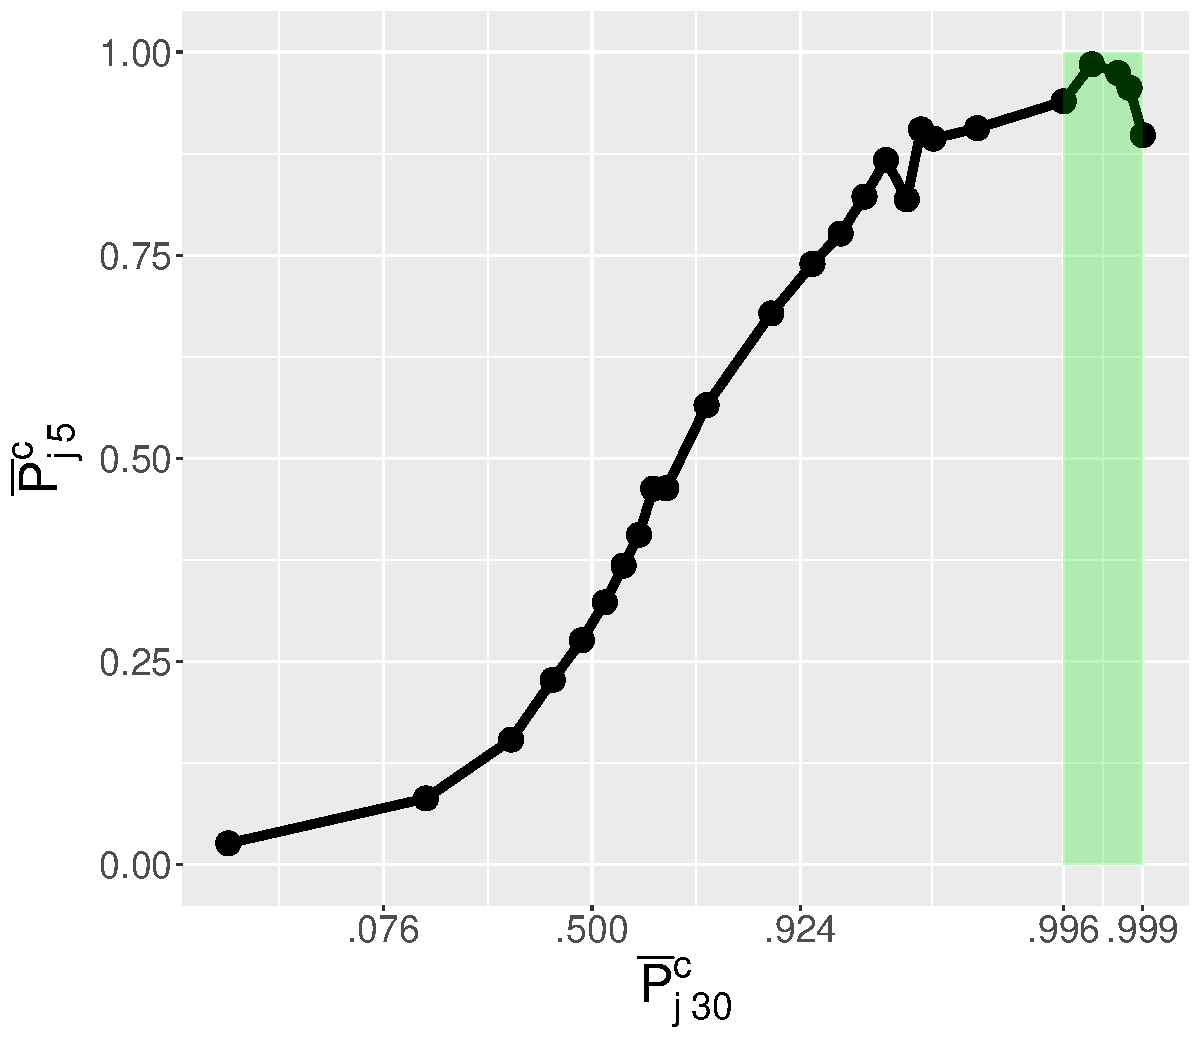
\includegraphics[width=\textwidth]{figures/pred_power/ncit_vs_pubrp/rp_rp.pdf}
         \caption{}
         \label{fig:pred_rp_rp}
     \end{subfigure}
        \caption{The predictability of citations and rank percentiles. The benchmark here is biology. Figure \ref{fig:pred_cit_age} and \ref{fig:pred_rp_age} show the citations and the corresponding rank percentiles for papers that have $50$ citations by age $5$. Figure \ref{fig:pred_cit_cit} displays the average citations by age $5$ over the average citations by age $30$, for different sets of publications, which are pre-specified by dividing the range of $\bar{c}_{j 30}$ into equal intervals in the log scale. Figure \ref{fig:pred_rp_rp} shows the corresponding average rank percentiles for the same sets of publications. Note that we do not claim originality for these plots, as figures \ref{fig:pred_cit_age} and \ref{fig:pred_cit_cit} have been illustrated via a different dataset\supercite{Wang2013}.}
        \label{fig:pub_cit_rp_pred}
\end{figure}


% publication rank percentile, heat map of correlations
\begin{figure}[ht!]
    \centering
    \begin{subfigure}[b]{0.8\textwidth}
        \centering
             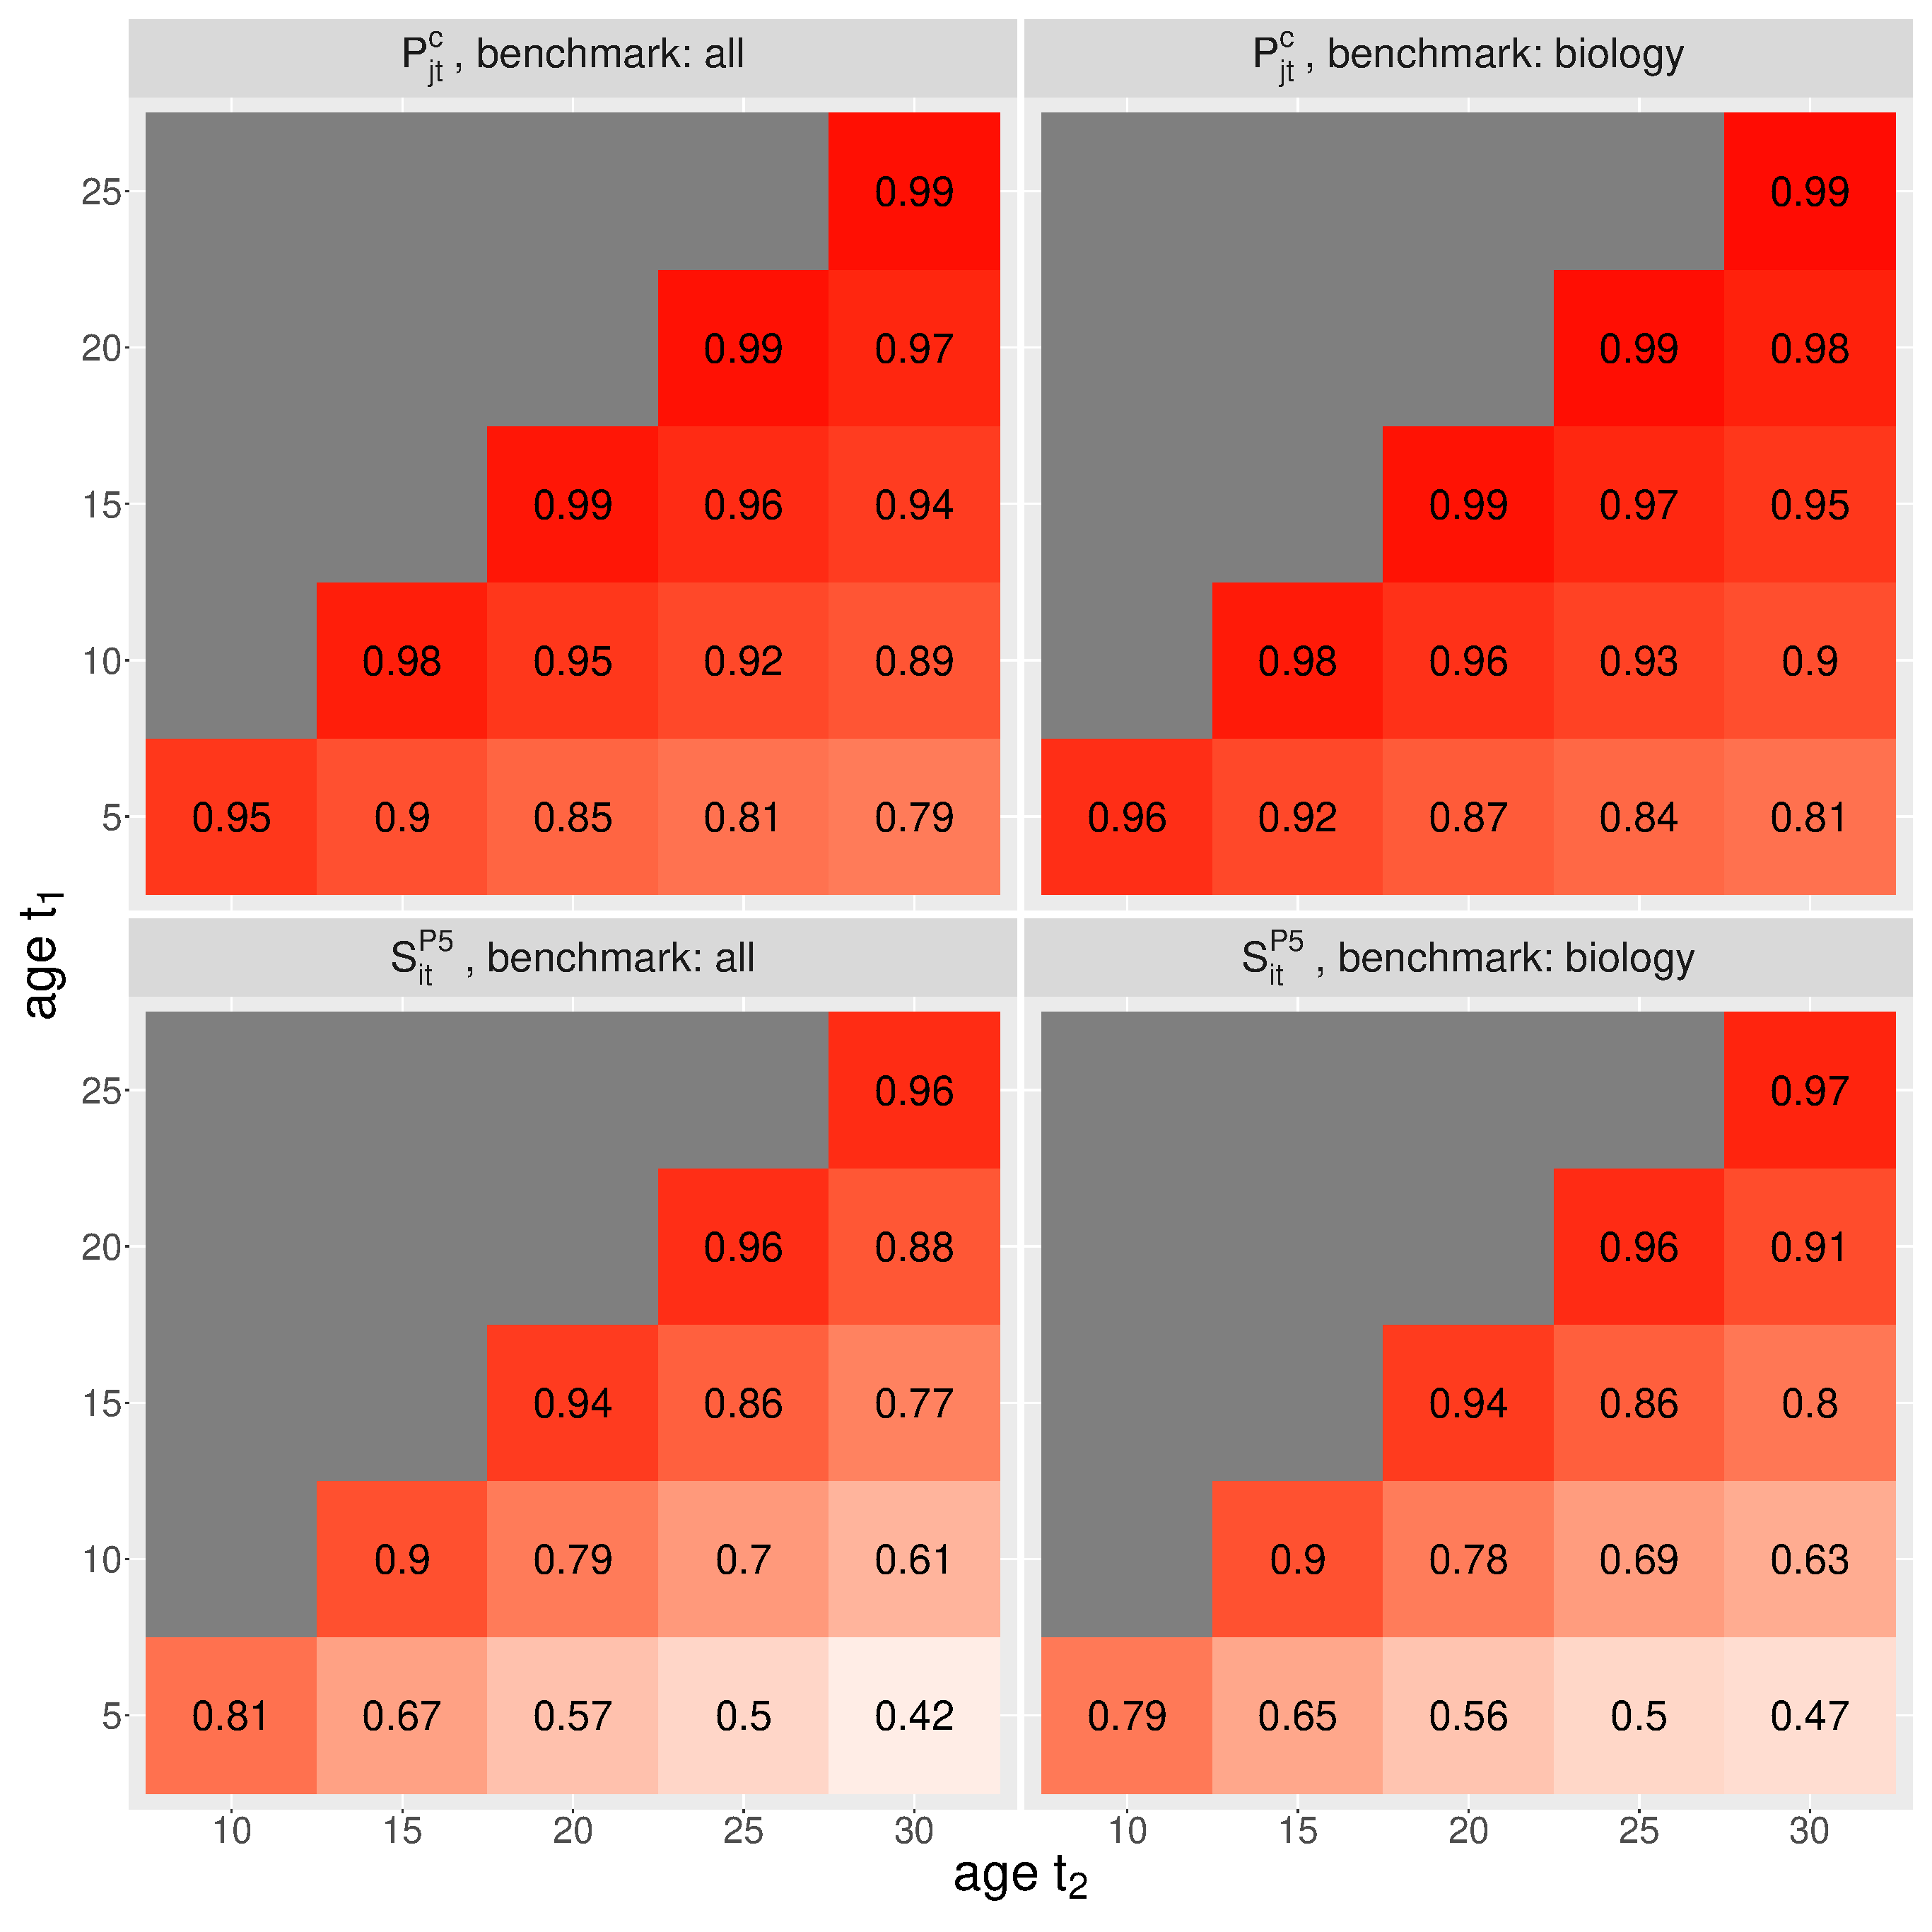
\includegraphics[width=\textwidth]{figures/pred_power/current/heatmap_cor.eps}
         \caption{Predict the cumulative impacts}
         \label{fig:hm_rp_current}
    \end{subfigure}
    
    \begin{subfigure}[b]{0.8\textwidth}
        \centering
             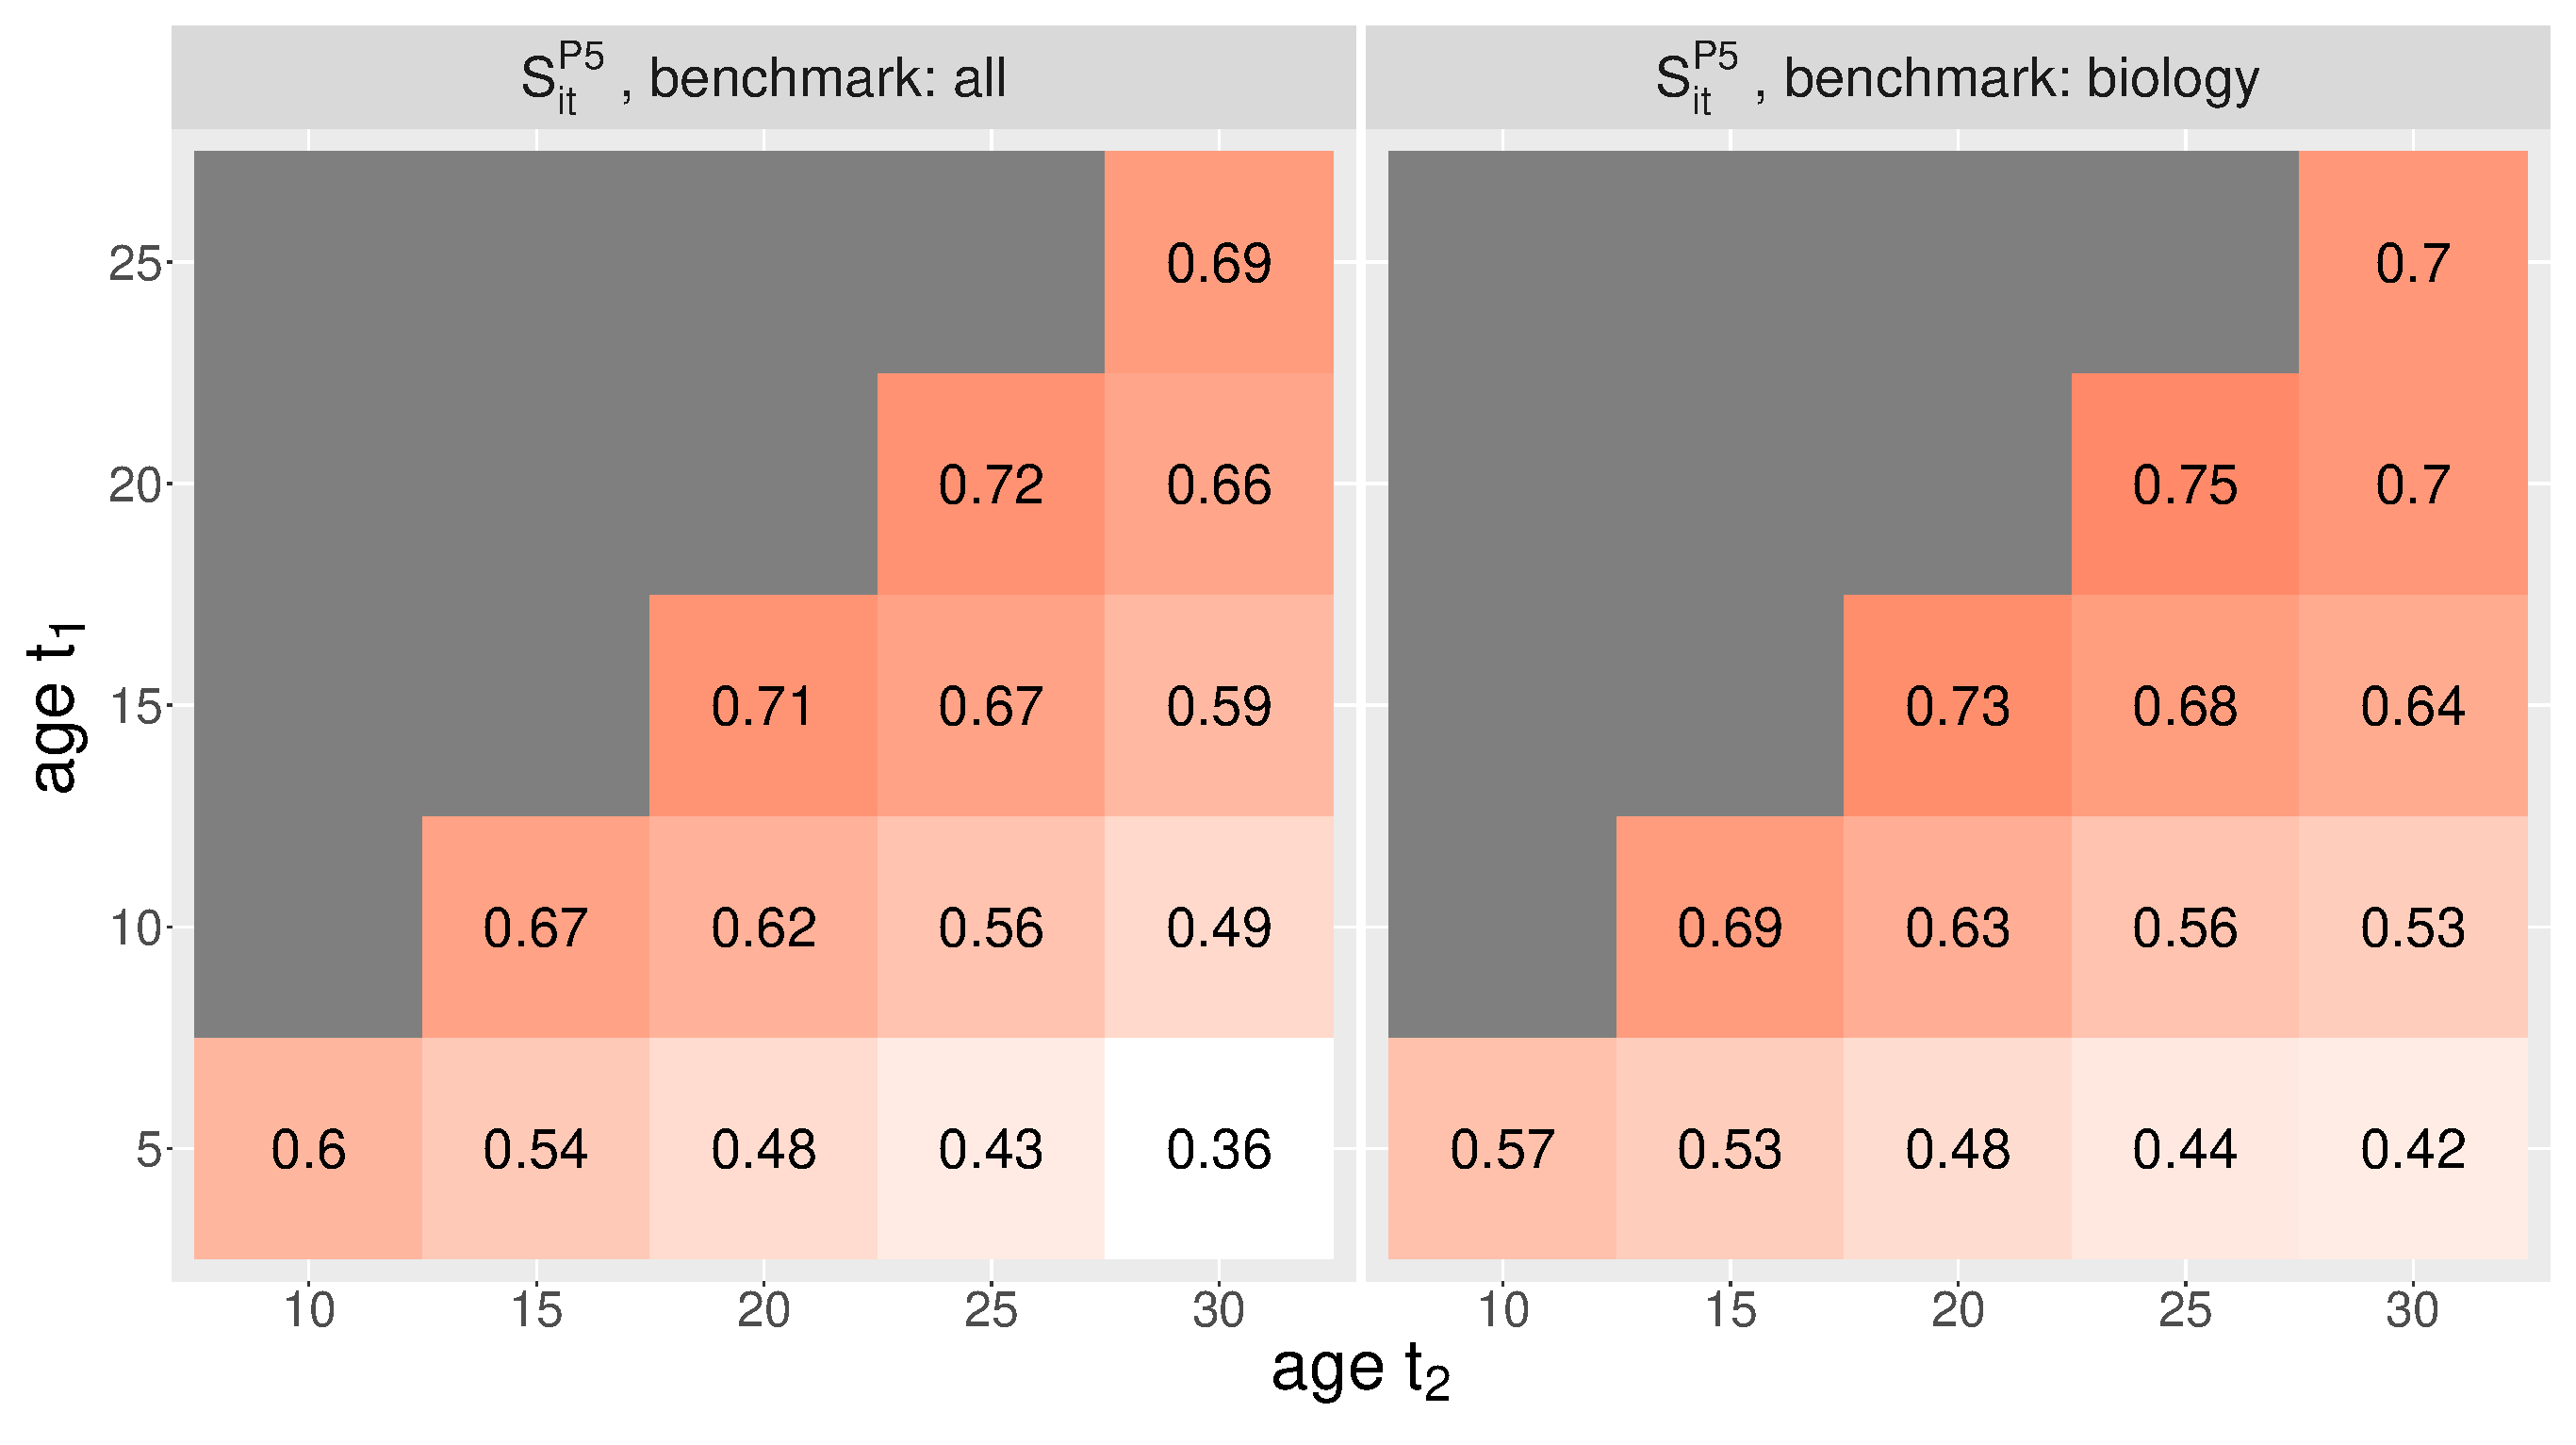
\includegraphics[width=\textwidth]{figures/pred_power/future/heatmap_cor.eps}
         \caption{Predict the future scientific output}
         \label{fig:hm_rp_future}
    \end{subfigure}
    \caption{The Pearson's correlation between RP indicators at two different ages. }
    \label{fig:hm_rp}
\end{figure}
\begin{figure}[ht!]
    \centering
    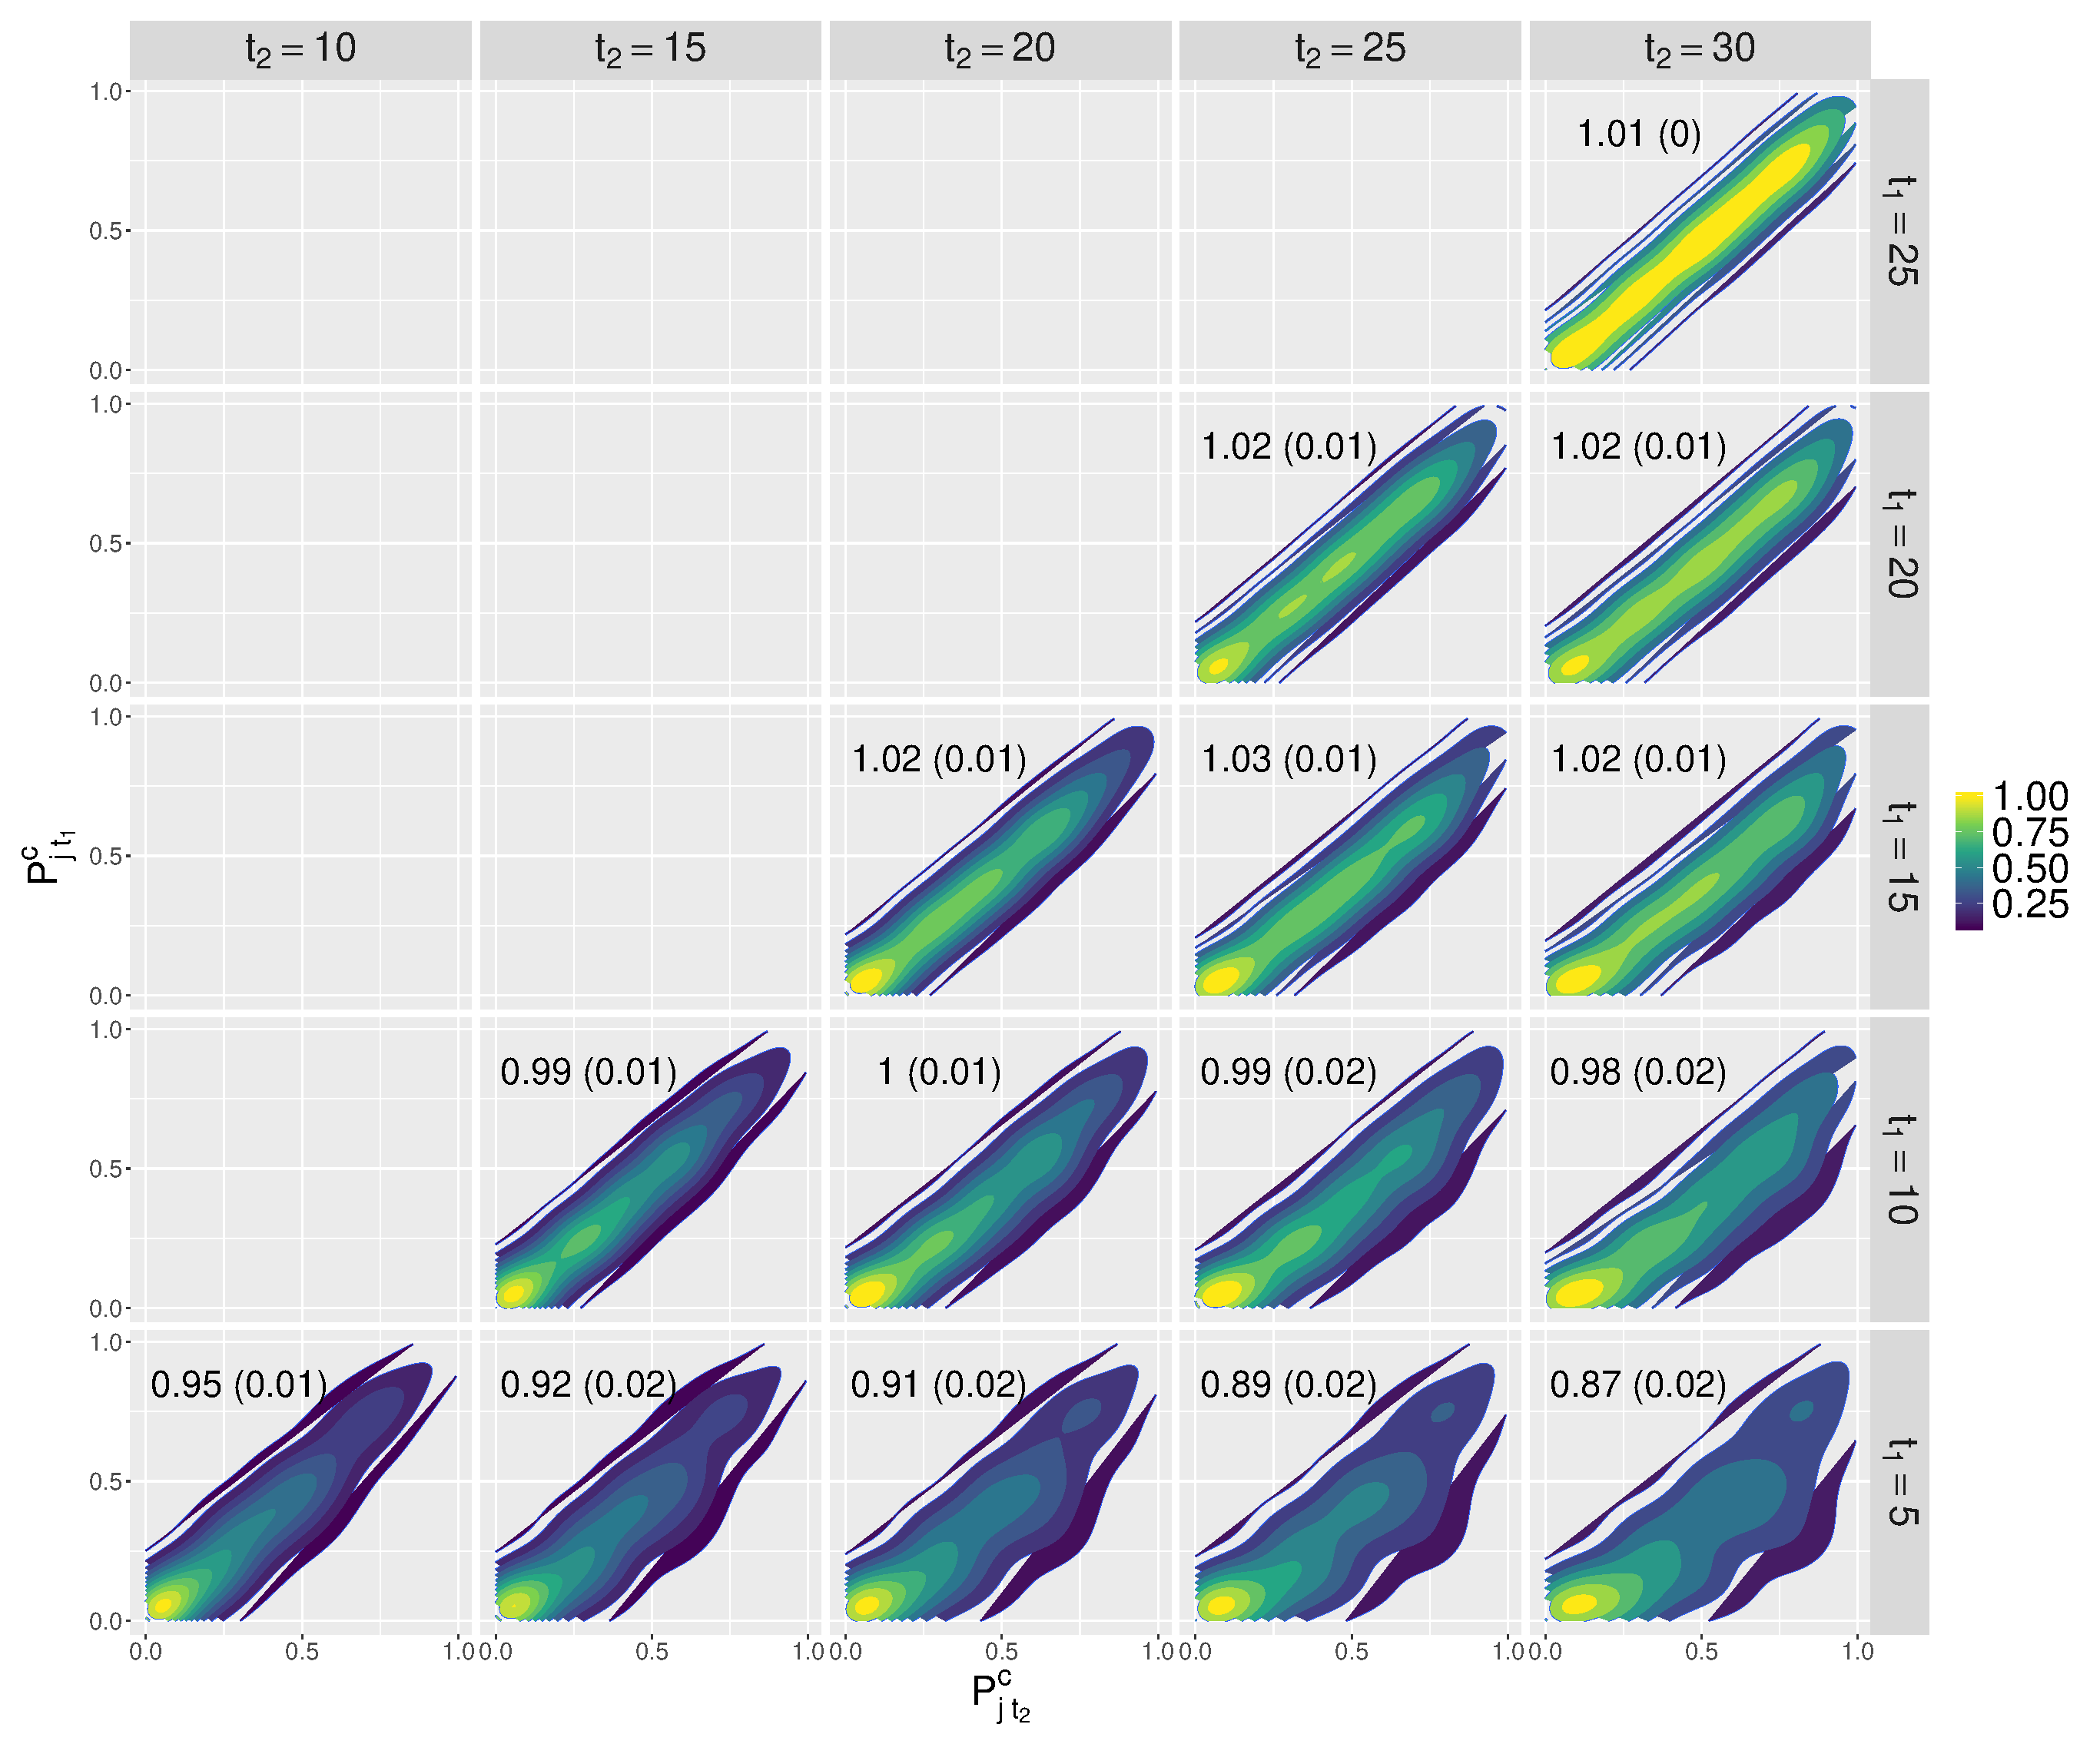
\includegraphics[width=\textwidth]{figures/pred_power/pubrp/scatter_bio1980.eps}
    \caption{Kernel density estimation of the scatters of P$_{j t_1}^c$ and P$_{j t_2}^c$. Meanwhile, we fit a simple linear regression of P$_{j t_2}^c$ upon P$_{j t_1}^c$. The estimated coefficient and the corresponding standard error (in the bracket) are displayed in each facet. The benchmark here includes all publications in biology and written in $1980$.}
    \label{fig:scatter_pubrp_bio1980}
\end{figure}


\begin{figure}[ht!]
    \centering
    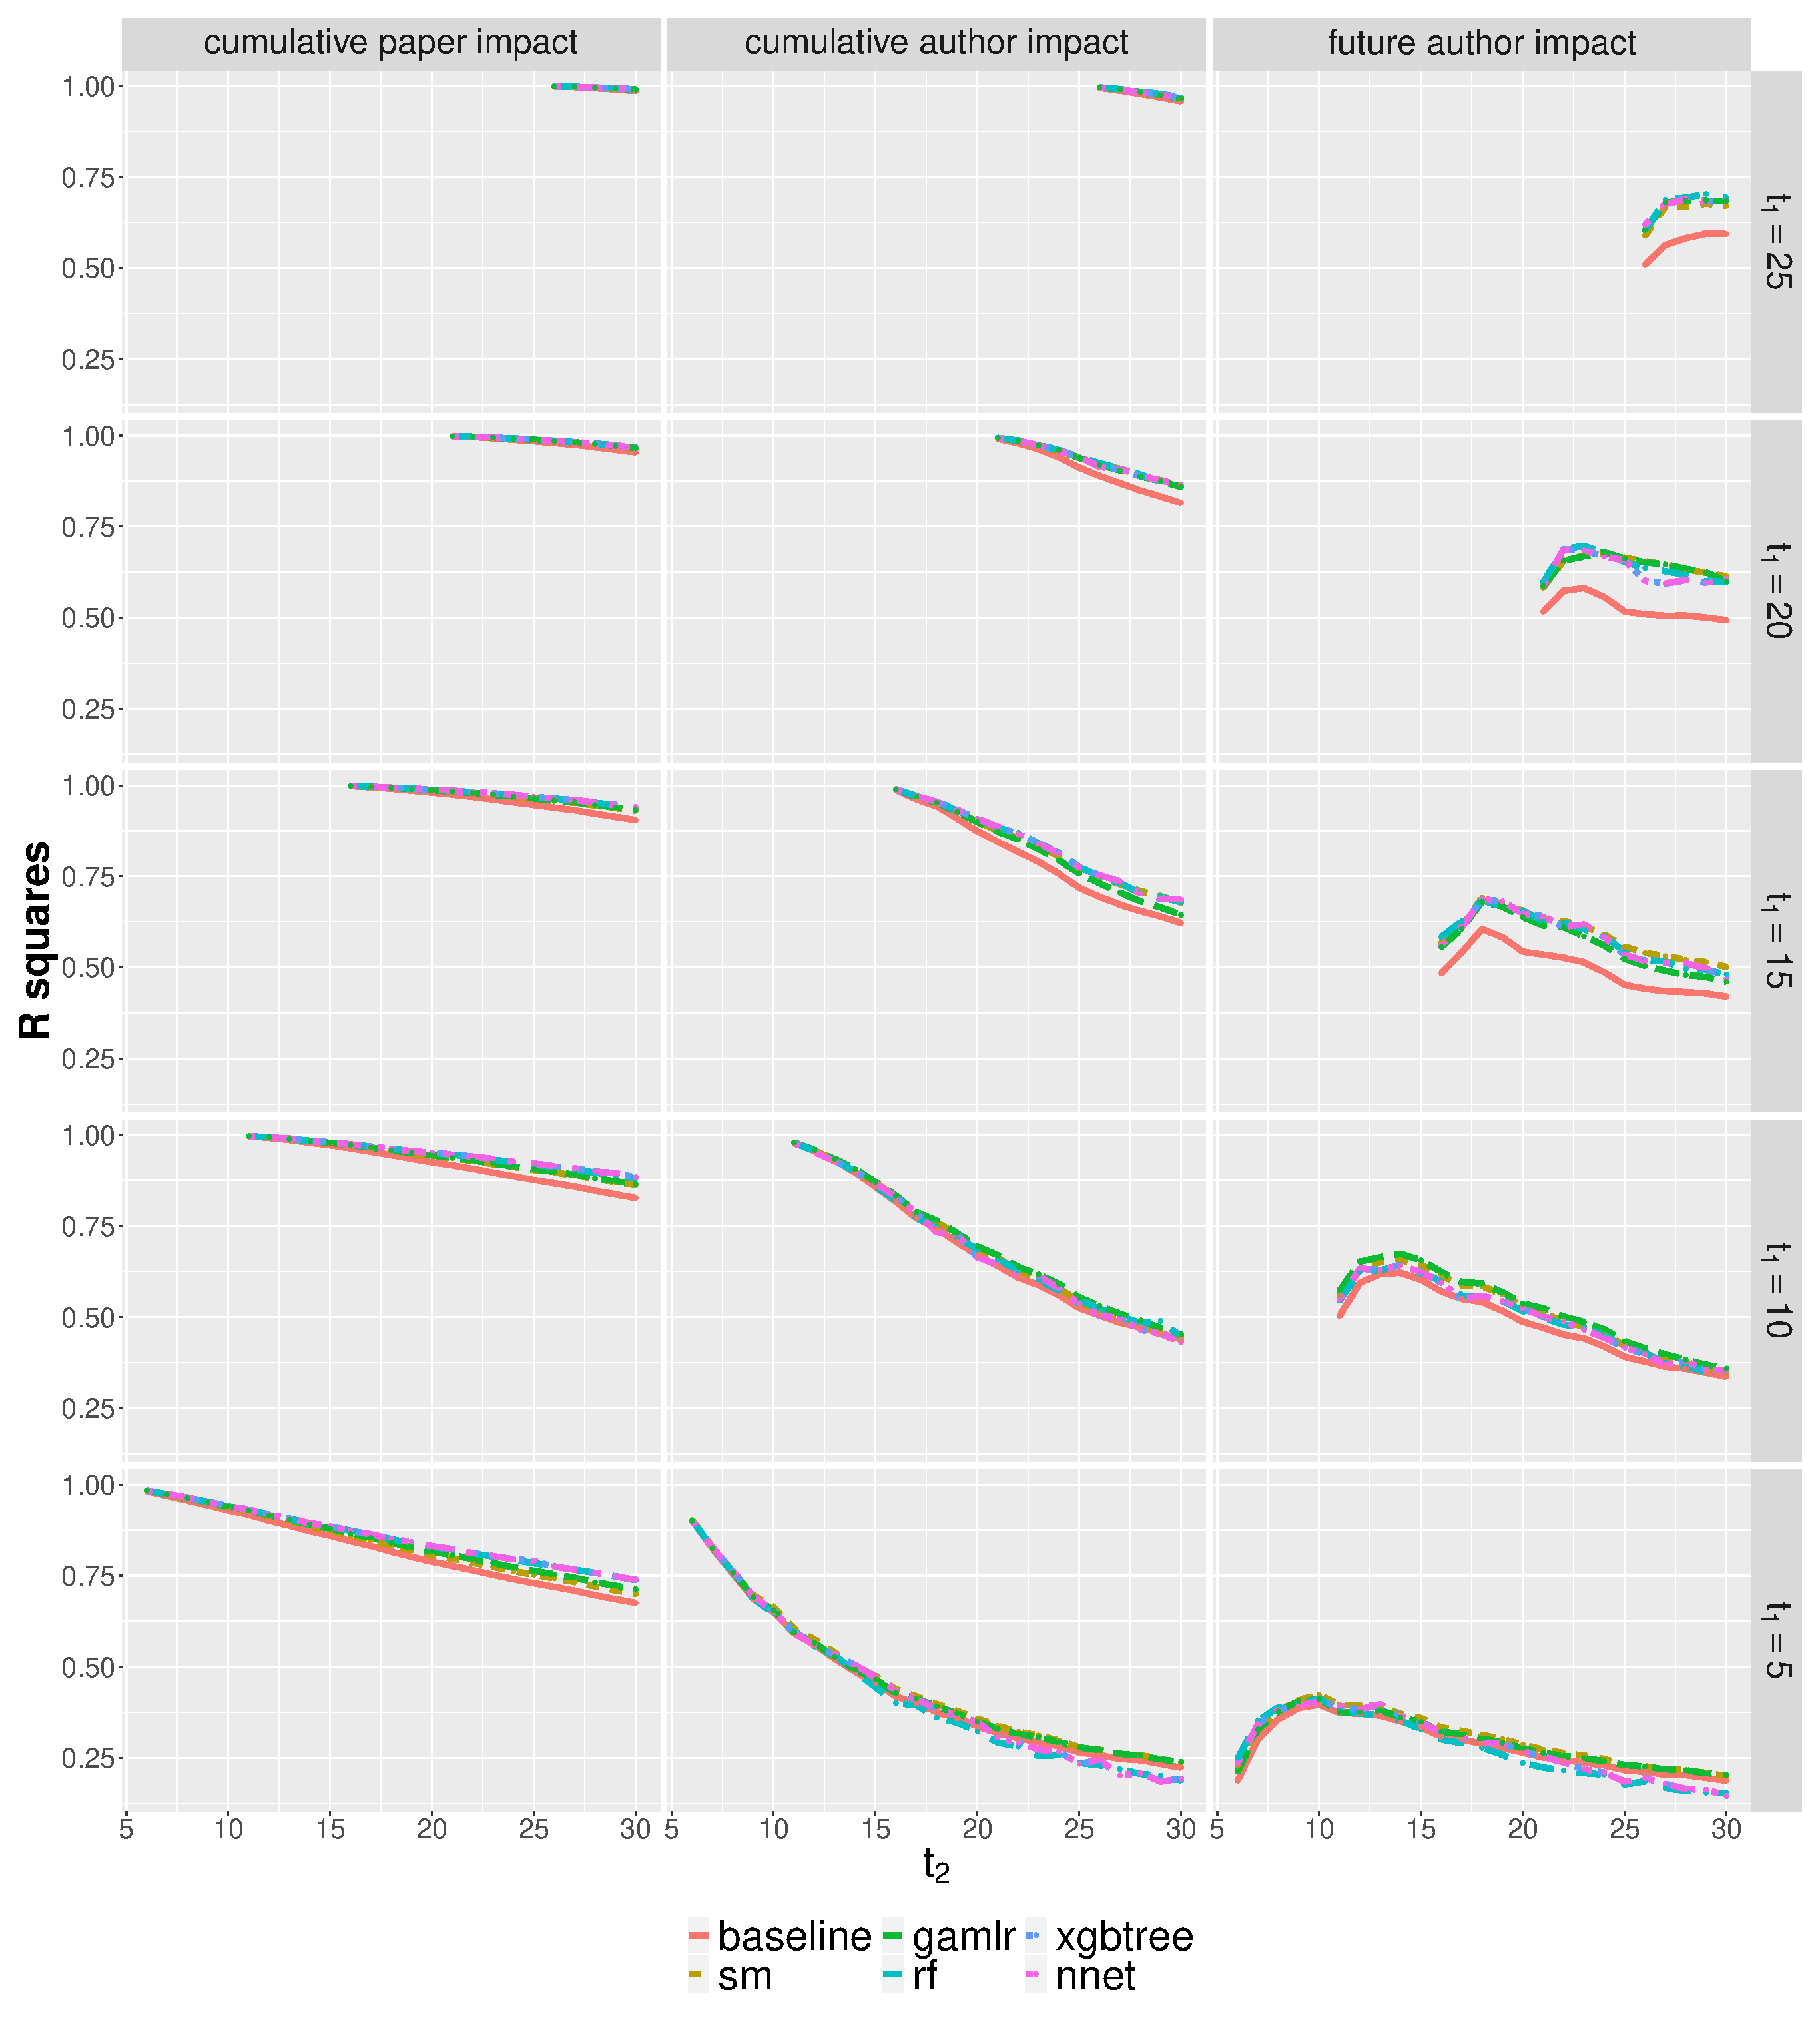
\includegraphics[width=\textwidth]{figures/pred_model/r2_diff.eps}
    \caption{Testing R squares of the predictive models. LASSO, ridge and elastic net are outperformed by Gamma LASSO, and hence are ignored for a better visualization.}
    \label{fig:pred_r2}
\end{figure}


\subsection*{A discussion on various types of rank percentile indicators for scholars}
S$_{it}^{c,b}$, S$_{it}^{h,b}$ and S$_{it}^{P5,b}$ are built upon an aggregation of the performances of the papers that the scholar publish by age $\tau$. S$_{it}^{c,b}$ and S$_{it}^{h,b}$ use the citations $c_{jt}$ to evaluate publication $j$ while S$_{it}^{P5,b}$ uses P$_{j5}^{c,b}$, i.e. the rank percentile of publication $j$ at age $5$. Meanwhile, the aggregation function for S$_{it}^{c,b}$ and S$_{it}^{P5,b}$ is sum, and it's a threshold function for S$_{it}^{h,b}$. 

S$_{it}^{P5,b}$ improves the major drawbacks of the other two indicators. First, it removes the seniority effect of publications, by evaluating the publications by their performances at age $5$. However, both the citations c$_{it}$ and h-index h$_{it}$ are dominated by 'senior' publications and newly published works can hardly contribute. Second, it improves over S$_{it}^{c,b}$ since it hardly rewards authors who publish a large number of low-impact works or only participate in a small number of high-impact projects. Similar to the h-index, the evaluation metric m$_{it}$ of rp.rp5 limits the contribution of a single publication to be at most $1$ due to the definition of rank percentile. However, the absolute number of citations is unlimited and is highly influenced by extreme values. Last, by comparing with rp.h, it penalizes authors who are not truly innovative, but carefully massage their h-indices by publishing a number of papers that are not top-class but attract just enough amount of citations to boost the h-index. As long as a paper is among the top h papers, the actual number of citations is irrelevant for rp.h, but it still affects rp.rp5.

We demonstrate these advantages of rp.rp5 by examining some extreme cases. We create three synthetic academic careers. Author A publishes a substantial number of publications at each age (more than $90\%$ of other authors in the benchmark), while all of the publications have little impacts. Meanwhile, author B and author C only publish $1$ paper at the beginning of their careers, where author B's paper is astonishing while author C's is average. All three authors have h-index as $1$ throughout their careers. Figure \ref{fig:simulated_authors} shows the author rp for these three artificial authors. We see that for author A and B, rp.c is substantially larger than the other two, and it dies down slowly. Even though author B only publishes one ground-breaking paper, the author remains in the top $50\%$ even by age $12$. Both rp.rp5 and rp.h are better characterizing the performances of these authors. Meanwhile, author C has the same rp.h as author B although his/her publication has much less impact. In this case, rp.rp5 and rp.c are better especially at the beginning of the careers. 

Besides these special cases, for the majority of authors in our dataset, we see a large agreement between rp.rp5 and the other two types of rp. Consider the benchmark being biology. In order to study the agreement, for each indicator, we classify the authors into four classes, class $1$: $0\le \text{rp} < 0.25$, class $2$: $0.25\le \text{rp} < 0.5$, class $3$: $0.5 \le \text{rp} < 0.75$ and class $4$: $0.75 \le \text{rp} \le 1$. An agreement in the classification of an author is where two (or three) different rp belong to the same class. The overall agreement for all three rp is $51\%$ at age $5$ and $68\%$ at age $30$, i.e. about half of the authors result in the same classifications of the three rp at age $5$, while that number becomes around two third at age $30$. Figure \ref{fig:aut_rp_class} shows the detailed classifications for every pair of the three rp. As we can see that, the agreement increases with the age. Furthermore, rp.rp5 has large agreements with both rp.c and rp.h, that are $69\%$ and $67\%$ respectively at age $5$, and $71\%$ and $81\%$ respectively at age $30$. 

We've shown the advantage of using rp.rp5 over indicators like rp.c and rp.h. A remaining question is why we use rp.c$_{j5}$ rather than say rp.c$_{j10}$ to represent the quality of the paper. It turns out that rp.c$_{j\tau}$ is highly stable over ages, and rp.c$_{j5}$ is very close to rp.c$_{j10}$ for the majority of papers. This will be discussed in the section below. Therefore, we are using less citation information and get similar accuracies. Other choices involve taking the summary statistic of the entire history of rp.c$_{j\tau}$ ($\tau=1,\cdots,T_j$). For example, we can take the best performance along the history, i.e. $\displaystyle \max_{t=1,\cdots,T_j} \text{rp.c}_{jt}$. We demonstrate that the evaluation metric m$_{i\tau}$ formulated based on these alternatives is highly correlated with m$_{i\tau}$ formulated rp.c$_{j5}$. Furthermore, the rank percentile indicators based on these alternatives are not statistically different from rp.rp5. The details are discussed in the supplemental material section \ref{sec:robustness_rprp}.

\subsection*{Predictive power of rank percentile indicators}
Citations have been shown to lack long-term predictive power\supercite{Wang2013}. Figure \ref{fig:pred_cit_age} shows that publications with the same citations by age $5$, can have noticeably different citation paths and long-term effects. Meanwhile, exceptional and creative ideas can normally take longer to be appreciated by the community. As shown in figure \ref{fig:pred_cit_cit}, the correlation between short-term citations and long-term citations breaks down for most highly-cited papers (the shaded area). Such problems affect less for rank percentiles, as evidenced by figure \ref{fig:pred_rp_age} and \ref{fig:pred_rp_rp}. For the papers having rp.c$_{j 5} \approx 0.75$, their rp.c$_{j 30}$ are all above $0.5$. Meanwhile, the correlation between short-term and long-term rp is still very strong for the most highly-cited papers. 

Publication rp.c$_{j\tau}$ and scholar rp.rp5$_{i\tau}$ are highly predictive and stable over age. Figure \ref{fig:hm_rp_current} shows the ability of the indicators to predict their own values. We see an extremely high predictive power for rp.c, which indicates that a publication with high rp.c after $\tau_1$ ages is very likely to have high rp.c after $\tau_2$ ages where $\tau_2 > \tau_1$. Meanwhile, the predictive power dies down as the forecast horizon gets larger, which simply reflects the difficulty of long-term forecast. Also, the correlation becomes higher when we have a longer history of the publication, e.g. it increases from $0.79$ to $0.86$ as $\tau_1$ changes from $5$ to $10$ while keeping the forecasting horizon fixed at $\tau_2-\tau_1=5$. Finally, we see a slightly higher predictive power when we restrict the benchmark to only include publications in biology.

Similar patterns can be observed for rp.rp5 according to figure \ref{fig:hm_rp_current}, although it has lower predictive power than rp.c. To be more specific, it starts with a high predictive power but dies down fast as the forecast horizon becomes larger. For instance, the correlation drops from $0.99$ to $0.94$ for rp.c while it decreases from $0.94$ to $0.77$ for rp.rp5, by fixing $\tau_1=15$. This is result from the fact that forecasting future impact of future works is considerably harder than forecasting the future impact of existing works. Predicting rp.c$_{j\tau_2}$ belongs to the latter. On the other hand, rp.rp5$_{i\tau_2}$ is based on the set of papers that scholar $i$ publishes by age $\tau_2$, which contains papers published by $\tau_1$ and papers published in the period of $(\tau_1,\tau_2]$. Hence, predicting rp.rp5$_{i\tau_2}$ involves predicting the future impact of existing works as well as the future impact of future works. As the forecast horizon $\tau_2-\tau_1$ becomes larger, we potentially have more `predicting the future of future' to deal with that makes the task tougher. Meanwhile, other types of scholar rank percentile indicators, rp.c and rp.h, have very similar predictive powers with rp.rp5, which is illustrated in figure \ref{fig:hm_autrp_current}.

It turns out that not only do publication rp.c has high predictive power, it's stable over age, i.e. rp.c$_{j\tau_1}\approx$rp.c$_{j\tau_2}$. Figure \ref{fig:scatter_pubrp_bio1980} shows the kernel densities of the scatters of rp.c$_{j\tau_1}$ vs rp.c$_{j\tau_2}$. We see that the scatters are mostly along the $45$ degree line. Meanwhile, we perform a simple linear regression by regressing rp.c$_{j\tau_2}$ upon rp.c$_{j\tau_1}$. The regression coefficient of variable rp.c$_{j\tau_1}$ together with the standard error is displayed besides each of the scatters in the figure. We see that the coefficients are very close to $1$ with very small standard errors, which gives further evidence that rp.c is stable over age. Meanwhile, figure \ref{fig:scatter_autrp_all} shows a similar study for the stableness of rp.rp5. We do not see strong evidence of rp.rp5 being stable over age.

We know that predicting rp.rp5 involves forecasting the future impact of both existing and future works. Such question can assist making decisions for a faculty position or tenureship, since the committee would like to examine the cumulative scientific impact of the scholar. A more difficult question is to predict the future impact of the future works. Such question is of interest, for example, in assigning research fundings or allocating research resources, where the future impact of existing works shall be irrelevant. Figure \ref{fig:hm_rp_future} shows the ability of using rp.rp5$_{i\tau_1}$ to predict rp.rp5$_{i\tau_2 \setminus \tau_1}$, where the latter is based on only the future papers, i.e. those written in the $(\tau_1,\tau_2]$ time interval. As expected, we see lower a predictive power than predicting rp.rp5$_{i\tau_2}$, but rp.rp5$_{i\tau_1}$ can still explain most of the variations in rp.rp5$_{i\tau_2 \setminus \tau_1}$ in relatively short horizons. 

\subsection*{Predictive models}
For both the publication and scholar impact, we've studied how well the performance by age $\tau_1$ predicts the cumulative achievement by age $\tau_2$. We demonstrate that rank percentile indicators (rp.c$_{j\tau}$ and rp.rp5$_{i\tau}$) have high predictive powers. Meanwhile for the scholar impact, we further investigate the prediction of performance in the subsequent $\tau_2-\tau_1$ ages, i.e. using rp.rp5$_{i\tau_1}$ to predict rp.rp5$_{i\tau_2 \setminus \tau_1}$. 

We now formulate these prediction tasks as supervised learning problems, and examine how much improvement we can get by having an extensive list of features and complex fitting algorithms. We consider the following fitting procedures; these models are ordered by increasing complexity, starting from simple baselines and ending with complex machine learning models:
\begin{itemize}
    \item Baseline: a simple linear regression of rp$_{\star \tau_2}$ upon rp$_{\star \tau_1}$.
    \item Simple Markov model (sm): a linear regression model of rp$_{\star \tau_2}$ upon features only including rp$_{\star \tau_1}$ and the change of rp over the last $2$ ages.
    \item Penalized linear regression models, including ridge\supercite{hoerl1970ridge}, LASSO\supercite{tibshirani1996regression}, elastic net (enet)\supercite{zou2005regularization} and the Gamma LASSO (gamlr)\supercite{taddy2017one}: linear models with different penalties on the regression coefficients. All of these methods shrink the coefficients towards zero, and the later three methods can provide sparse solutions (shrink the coefficients to exactly zeros). 
    \item Ensemble methods of regression trees, including random forest (rf)\supercite{liaw2002classification} and extreme gradient boosting trees (xgbtree)\supercite{chen2016xgboost}: rf is a bagging of regression trees with a subset of randomly selected features chosen at each split to avoid overfitting. xgbtree is a fast implementation of gradient boosting on regression trees with a model formation that emphasizes the role of regularizations to avoid overfitting.
    %\item Support vector regression (svr)\supercite{drucker1997support}: 
    \item Deep neural networks (dnn): feedforward networks with multiple hidden layers and using dropout and $l_2$ regularization to avoid overfitting.
\end{itemize}

\subsubsection*{Features and model fitting}
A crucial step for supervised machine learning models is feature engineering. The features that we create are based on the citation histories and are characterized into either author related or paper related features. For example, to predict the author impact rprp5$_{i\tau_2}$, an author related feature can be the number of papers that the author publish by age $\tau_1$, and a paper related feature can be the average citations of these papers. The $30$ features for predicting the publication impact and the $42$ features for predicting the author impact, are listed in tables \ref{tab:features_pubrp} and \ref{tab:features_autrp} respectively. 

The features are created only using the citation information available by $\tau_1$ and the response is specified at $\tau_2$. With a pair of features and response, all the models are trained and evaluated on the testing set, where the training and testing are randomly split in a 9-1 ratio. We consider $5$ different values of $\tau_1$ representing different stages of a publication or a scholar, that are $\tau_1\in\{5,10,15,20,25\}$, and for each $\tau_1$ we have $\tau_2=\tau_1+1,\cdots,30$, which results in $75$ pairs of $(\tau_1,\tau_2)$ in total. Hence all the models are trained $75$ times independently. Meanwhile, the machine learning models all rely on some hyper-parameters that require careful tuning. We use randomized searching with multiple iterations over a pre-specified parameter space, and the optimal set of hyper-parameters is chosen to minimum the 10-fold cross-validation error.

If we ignore the fact that we are modeling rp.c$_{j\tau}$ and rp.rp5$_{i\tau}$ at fixed time points, and view them as time series. Both series turn out to be non-stationary, based on statistical tests such as the Dicky-Fuller test\supercite{dickey1979distribution} and the KPSS test\supercite{kwiatkowski1992testing}, where the details are discussed in the supplemental material section \ref{sec:stationarity_test}. It's often encouraged to work on stationary series, for example in the autoregressive and moving average models, and a typical practice is to model differenced series. We follow the same logic here, and use the differenced series as the responses, e.g. $\Delta \text{rp.c}_{j\tau_2} = \text{rp.c}_{j\tau_2} - \text{rp.c}_{j\tau_1}$. 

\subsubsection*{Results}
We consider four evaluation metrics for the predictive models, that are the R squares ($R^2$), root mean squared error (RMSE), root median squared error (RMEDSE) and mean absolute error (MAE). The $R^2$ for all the models are shown in figure \ref{fig:pred_r2}, while the rest of the metrics are displayed in figure \ref{fig:pred_rmse}, \ref{fig:pred_medse} and \ref{fig:pred_mae}. We see that the baseline model predicts the cumulative impacts well, and the improvement of using more features and machine learning models have little benefit. Meanwhile, the baseline model can still provide reasonable predictions for the future scholar impact, although the machine learning models can provide better results when $\tau_1$ is relatively large. However, in such scenarios, the simple Markov model performs closely to the machine learning models, and hence the extensive list of features and complex non-linearity have little impact.






%\include{todo}
%\include{todiscuss}


\clearpage
%\bibliography{reference}
\printbibliography
%%!TEX root = main.tex
\clearpage
% fig:stableness_rp
% The rank percentile indicators are stable over publishing years 
\begin{figure}[ht!]
    \centering
    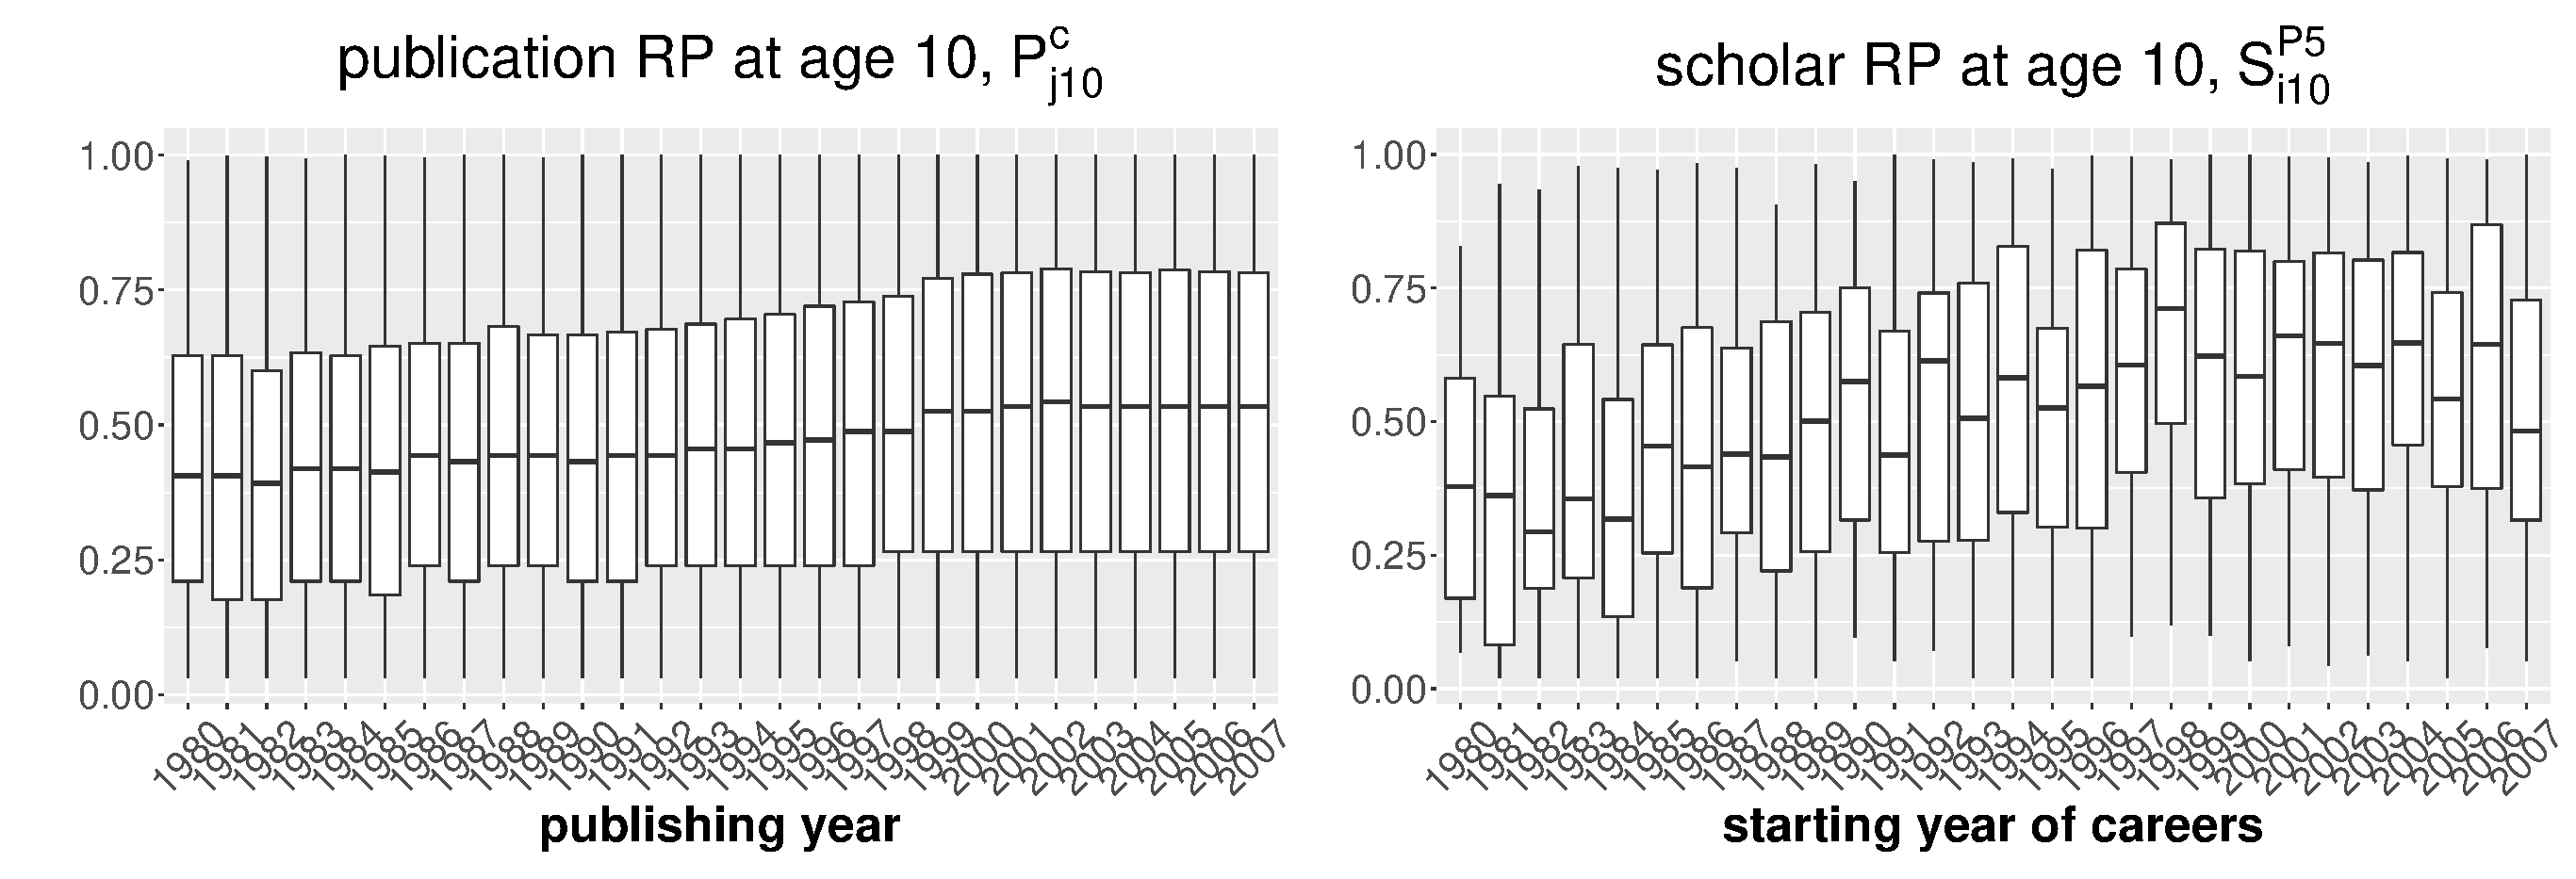
\includegraphics[width=\textwidth]{figures/exploratory/stationarity.eps}
    \caption{P$_{i10}^c$ grouped by the publication years and and S$_{i10}^{P5}$ grouped by the starting years of academic careers. The benchmark contains professors from various disciplines who receive their tenureships in year $2016$ or pubRP .}
    \label{fig:stableness_rp}
\end{figure}


% fig:panos
% show Panos as an example
\begin{figure}[ht!]
    \centering
    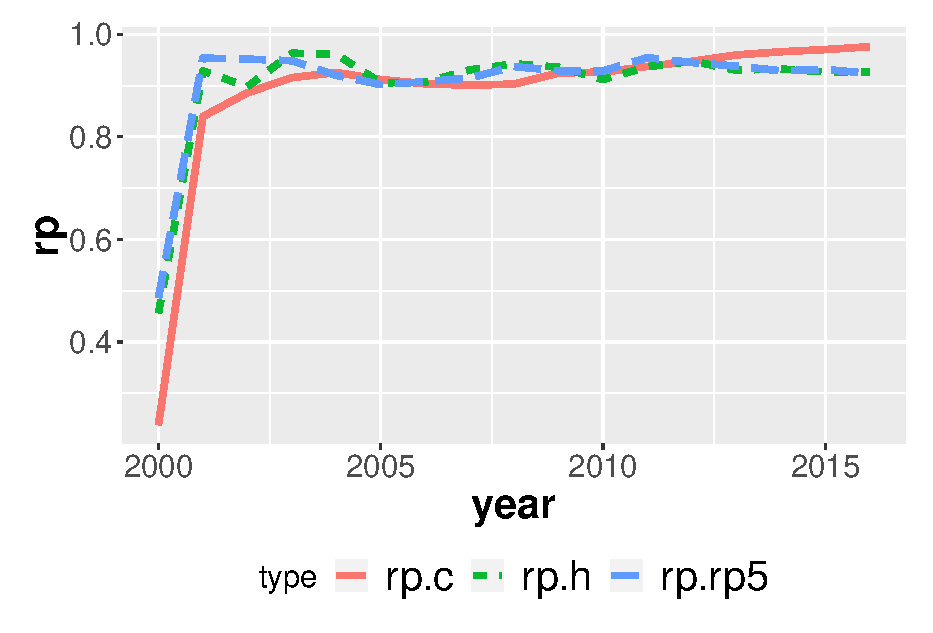
\includegraphics[width=0.7\textwidth]{figures/compare_autrp/panos.eps}
    \caption{The rank percentile indicators for Panos Ipeirotis. The benchmark contains all tenured professors by $2016$.}
    \label{fig:panos}
\end{figure}


% fig:simulated_authors
% show the difference between various author rp
\begin{figure}[ht!]
    \centering
    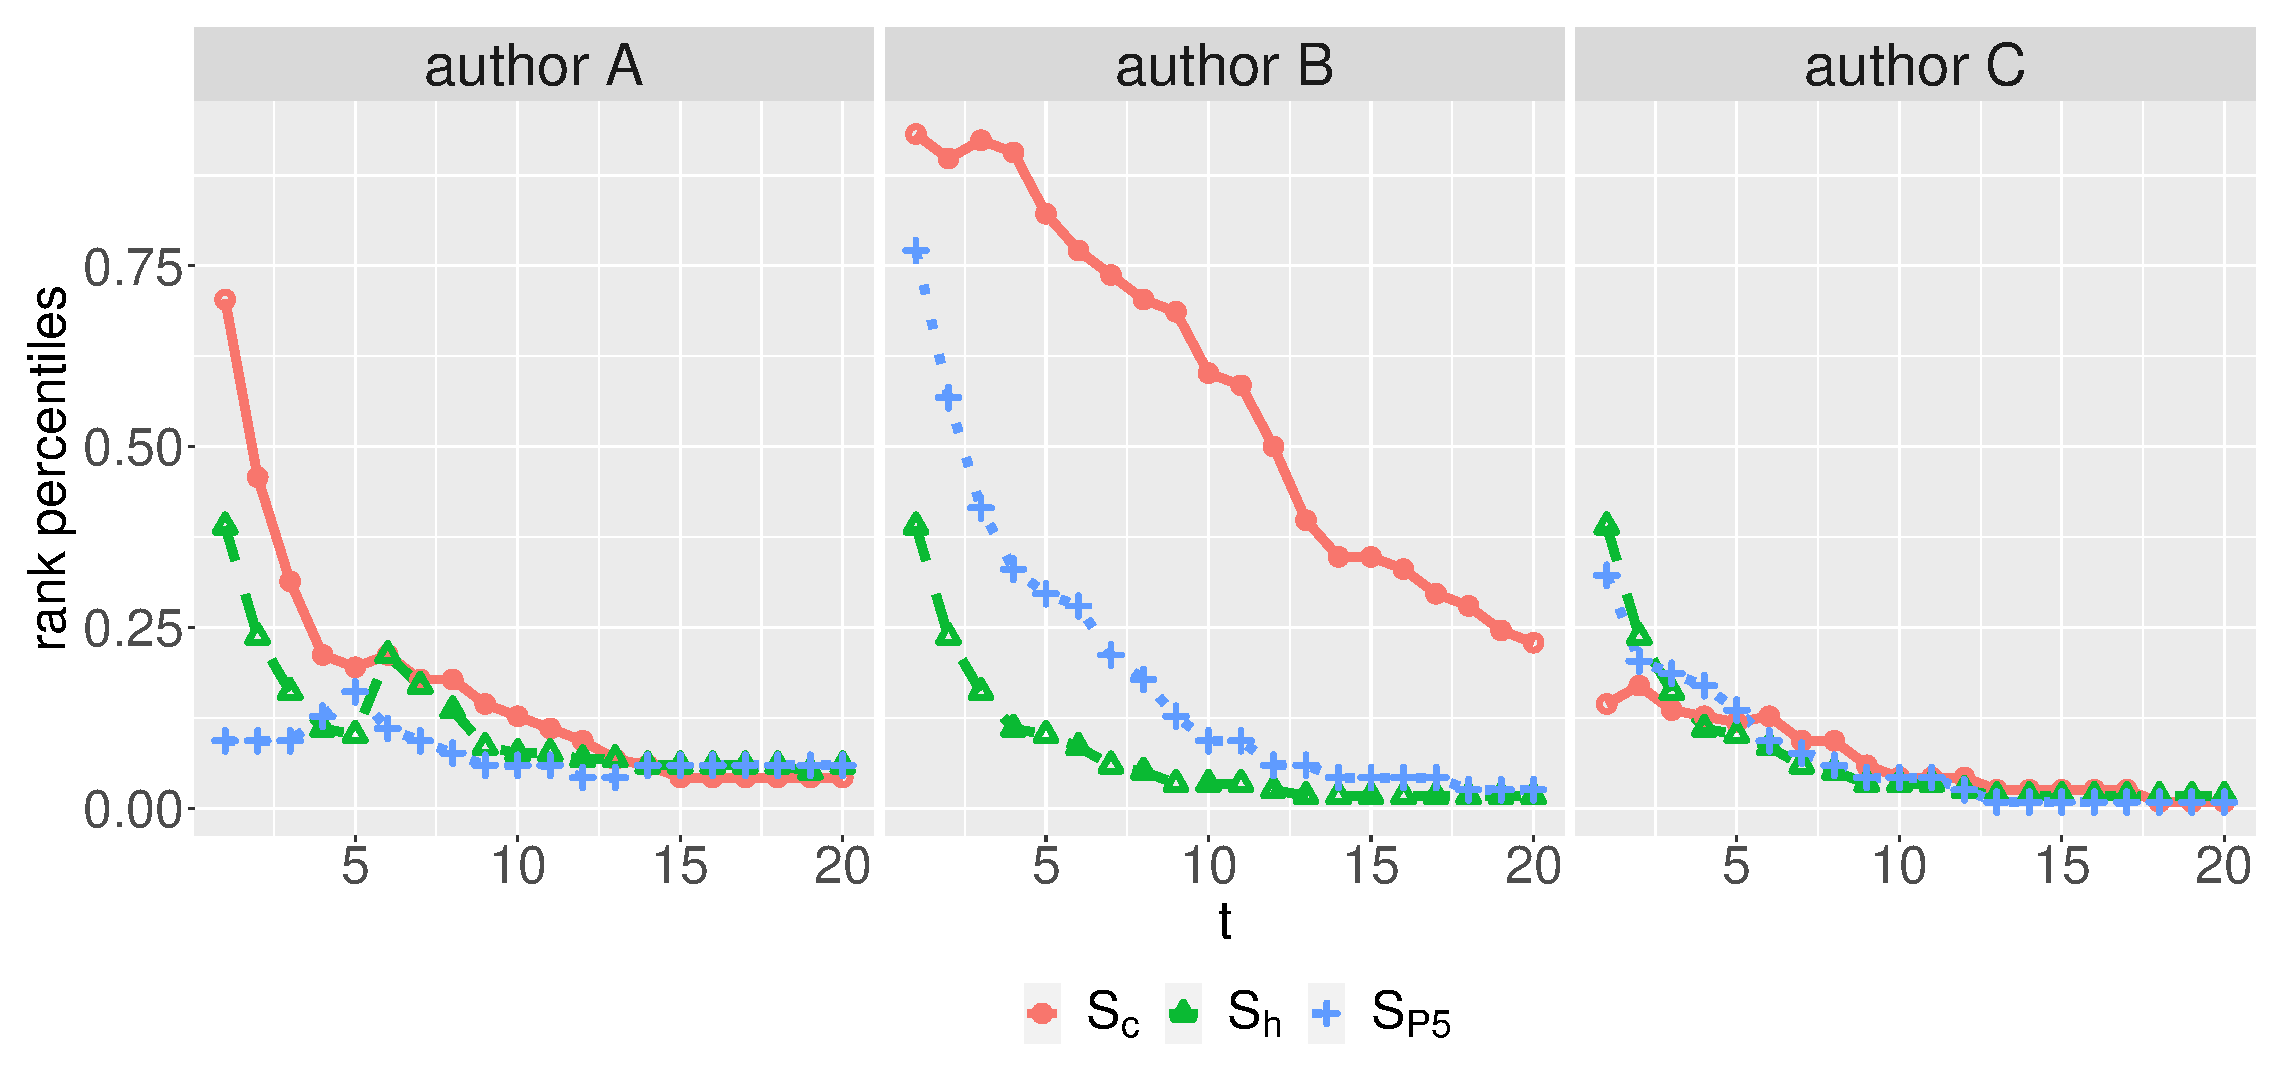
\includegraphics[width=\textwidth]{figures/compare_autrp/simulated_authors.eps}
    \caption{Three artificial authors to illustrate the difference between various types of author rank percentile indicators. Author A is highly productive at all ages but all of the works have little impact. Author B and author C only publish one paper at age $1$ throughout the entire careers, where the paper of author B has very high impact while the paper of author C has medium impact. The h-index of all authors at all ages are $1$. The benchmark contains authors in biology who start their careers from year $1990$.}
    \label{fig:simulated_authors}
\end{figure}


% fig:aut_rp_class
% class agreement among all the author rp
\begin{figure}[ht!]
    \centering
    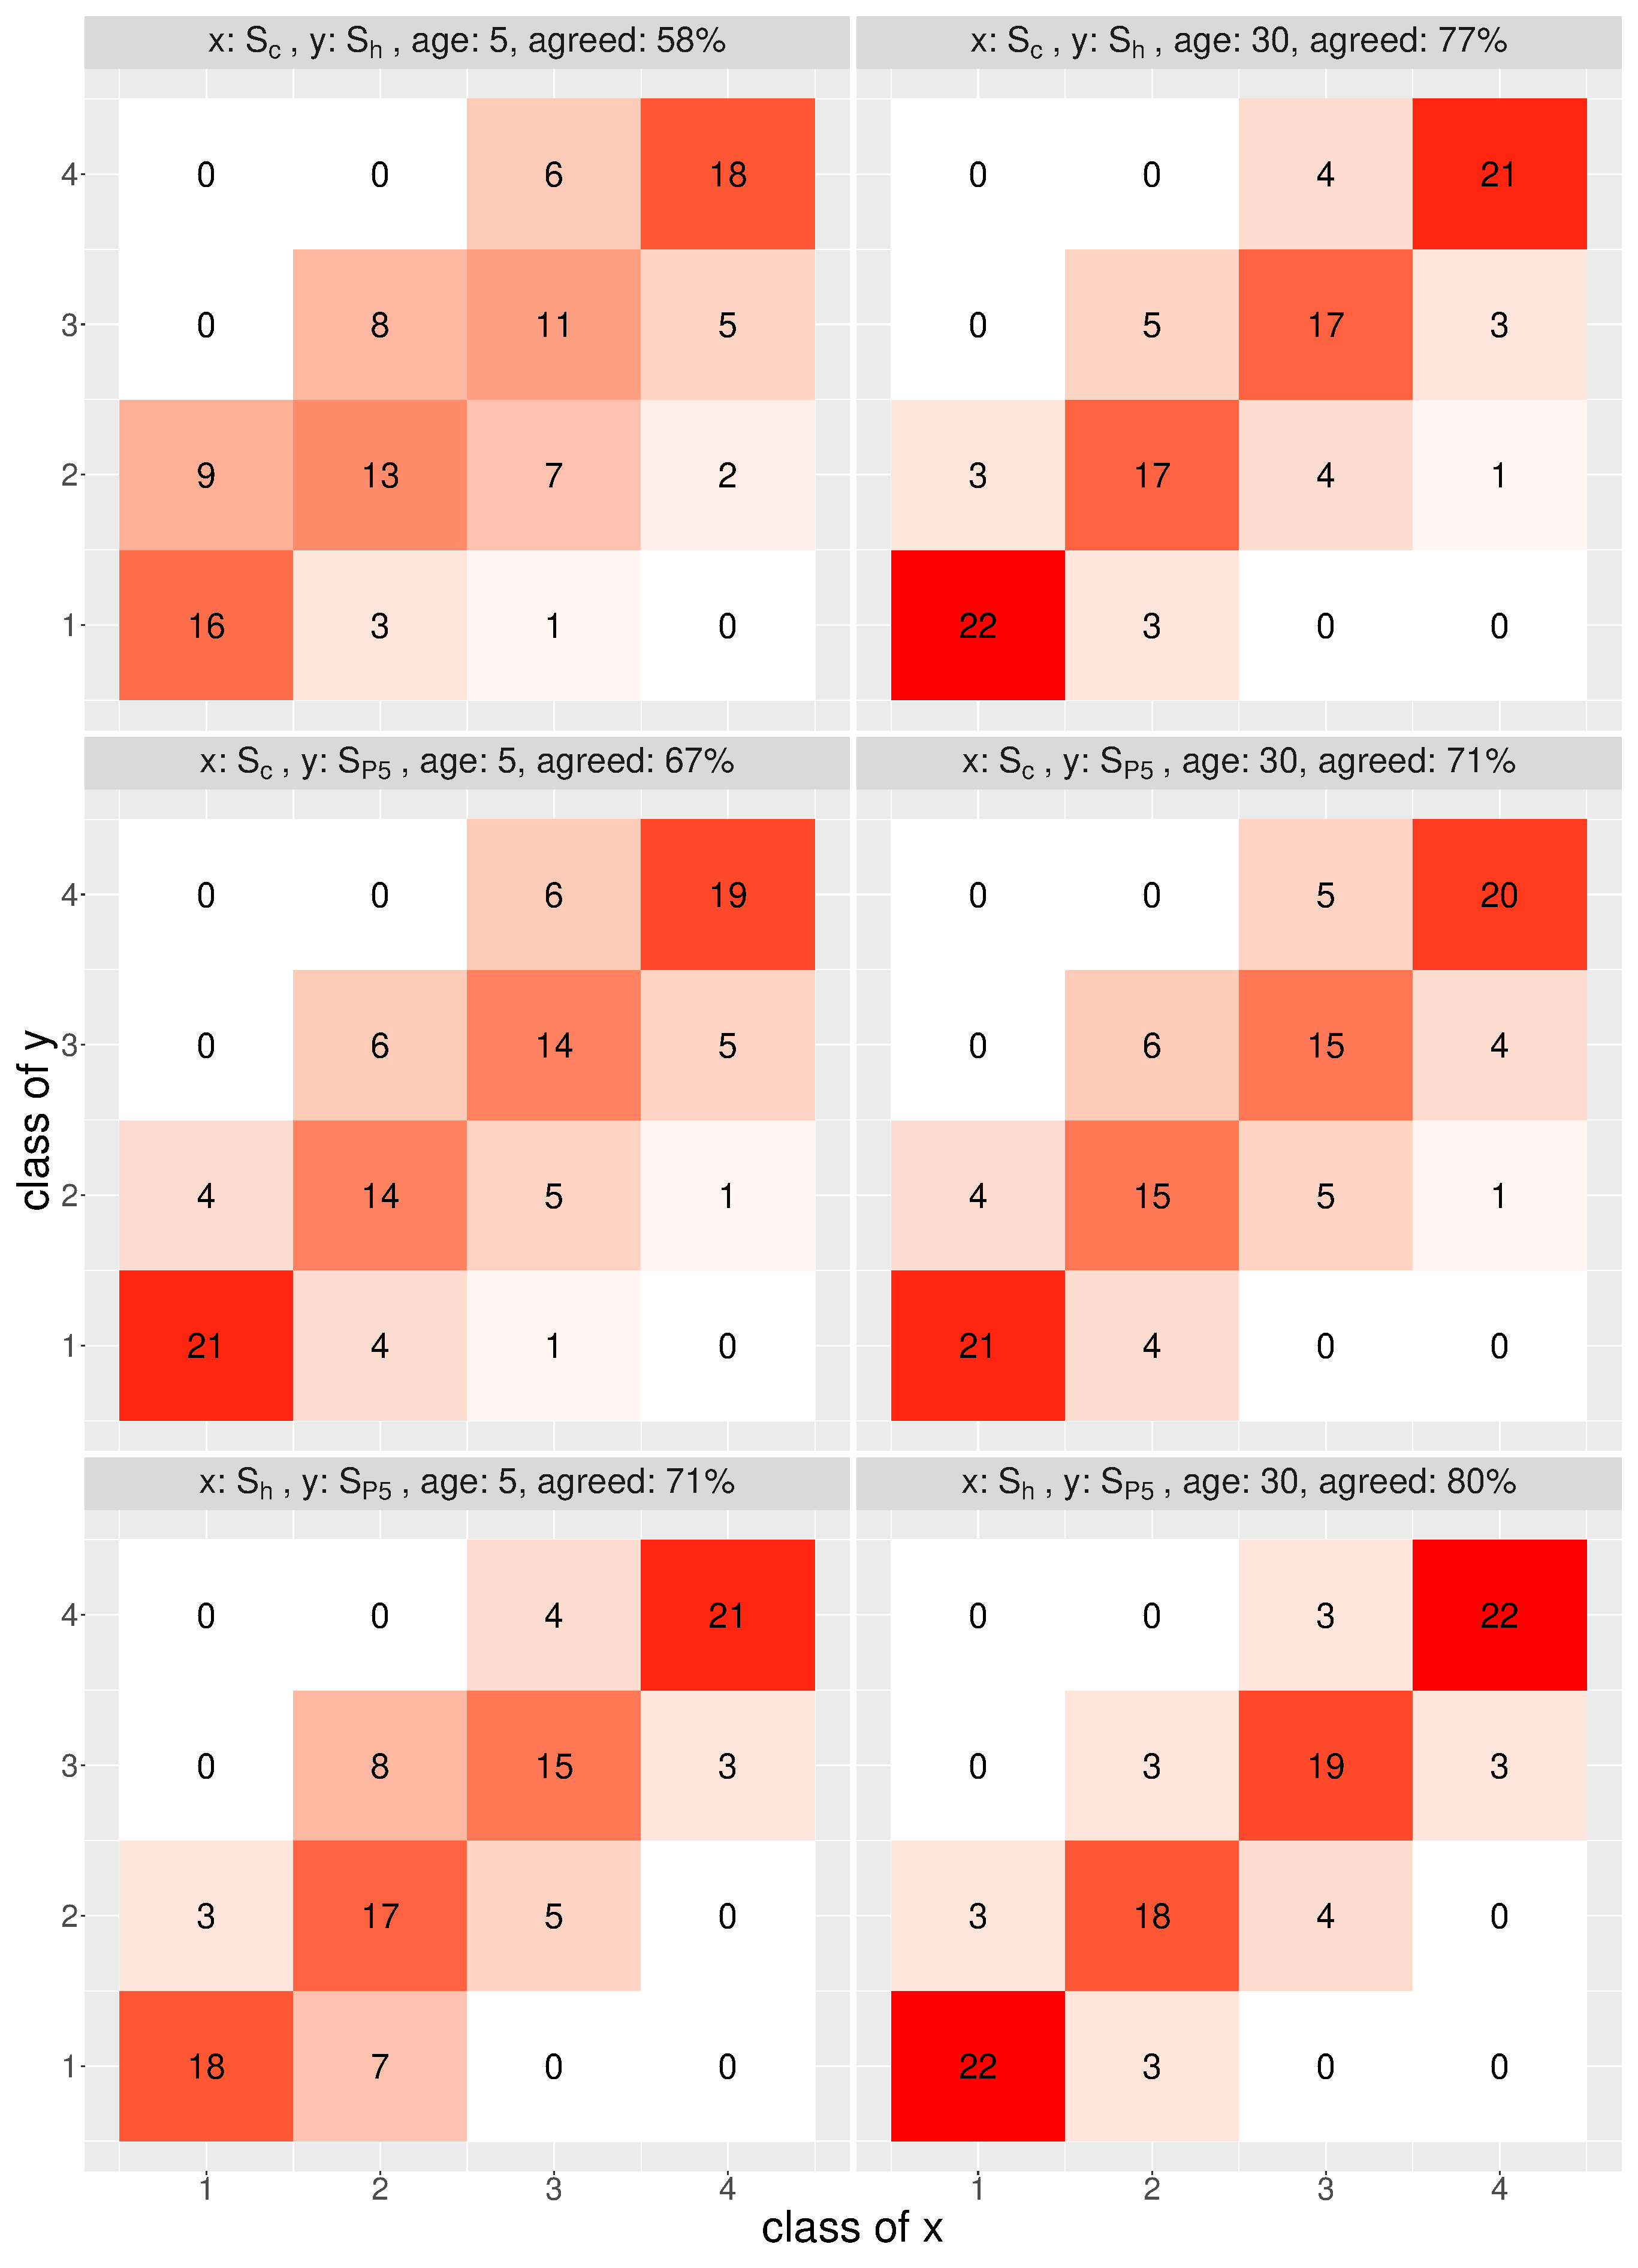
\includegraphics[width=0.88\textwidth]{figures/compare_autrp/heatmap_class_agreement.eps}
    \caption{Classifications of various types of author rp. Each rp is classified into four classes, class 1: $0 \le \text{rp} < 0.25$, class 2: $0.25 \le \text{rp} < 0.5$, class 3: $0.5 \le \text{rp} < 0.75$ and class 4: $0.75 \le \text{rp} \le 1$. The agreement of classifications (sum of the anti-diagonal elements) is displayed in the title of each panel. The benchmark is biology. The agreement for all three types is $51 \%$ at age $5$ and $68 \%$ at age $30$.}
    \label{fig:aut_rp_class}
\end{figure}

% publication rank percentile vs citations, predictability, Wang(2013)
\begin{figure}
     \centering
     \begin{subfigure}[b]{0.48\textwidth}
         \centering
         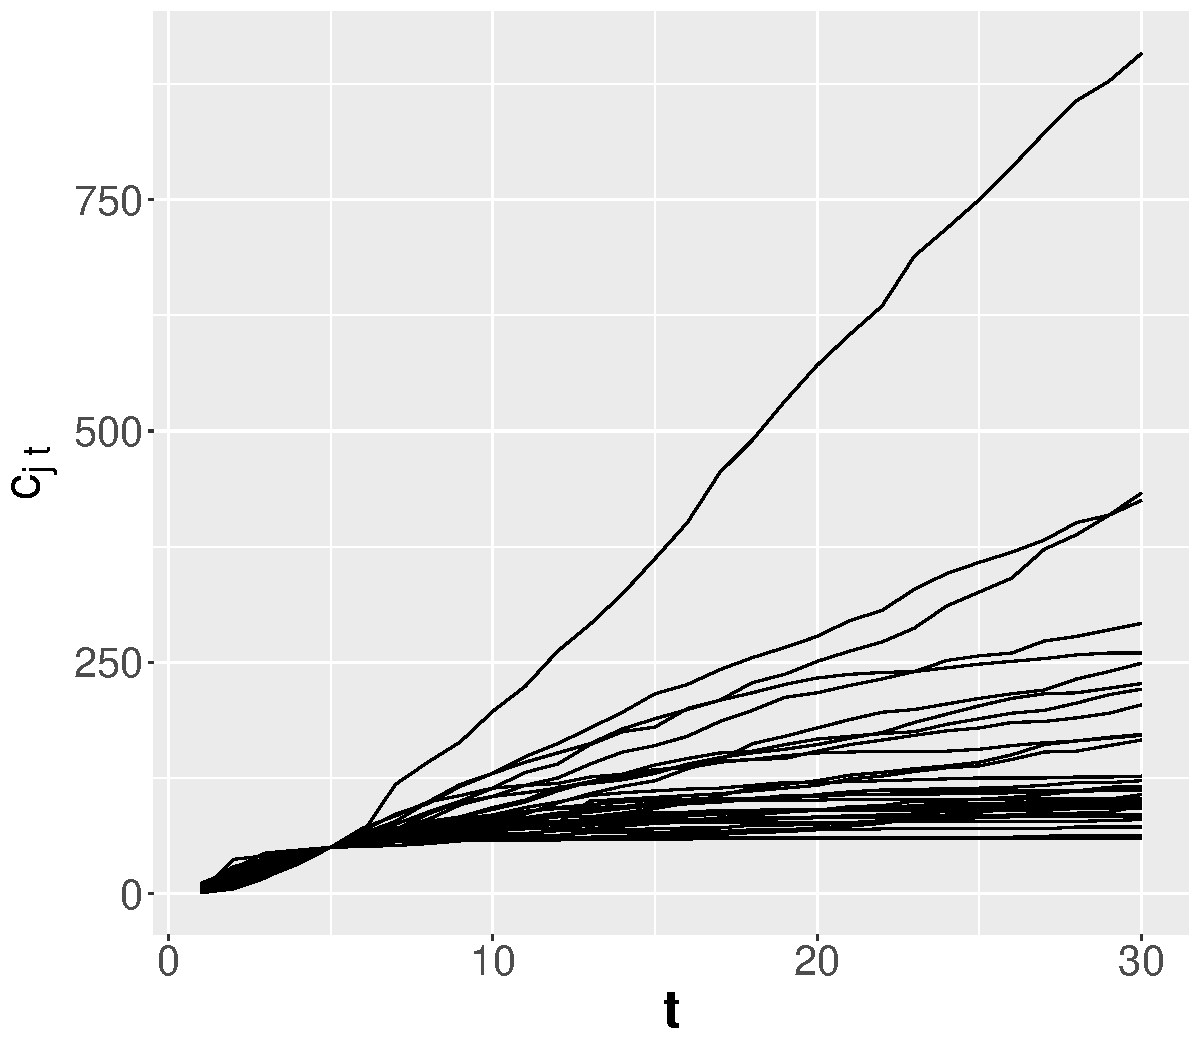
\includegraphics[width=\textwidth]{figures/pred_power/ncit_vs_pubrp/cit_age.pdf}
         \caption{}
         \label{fig:pred_cit_age}
     \end{subfigure}
     \hfill
     \begin{subfigure}[b]{0.48\textwidth}
         \centering
         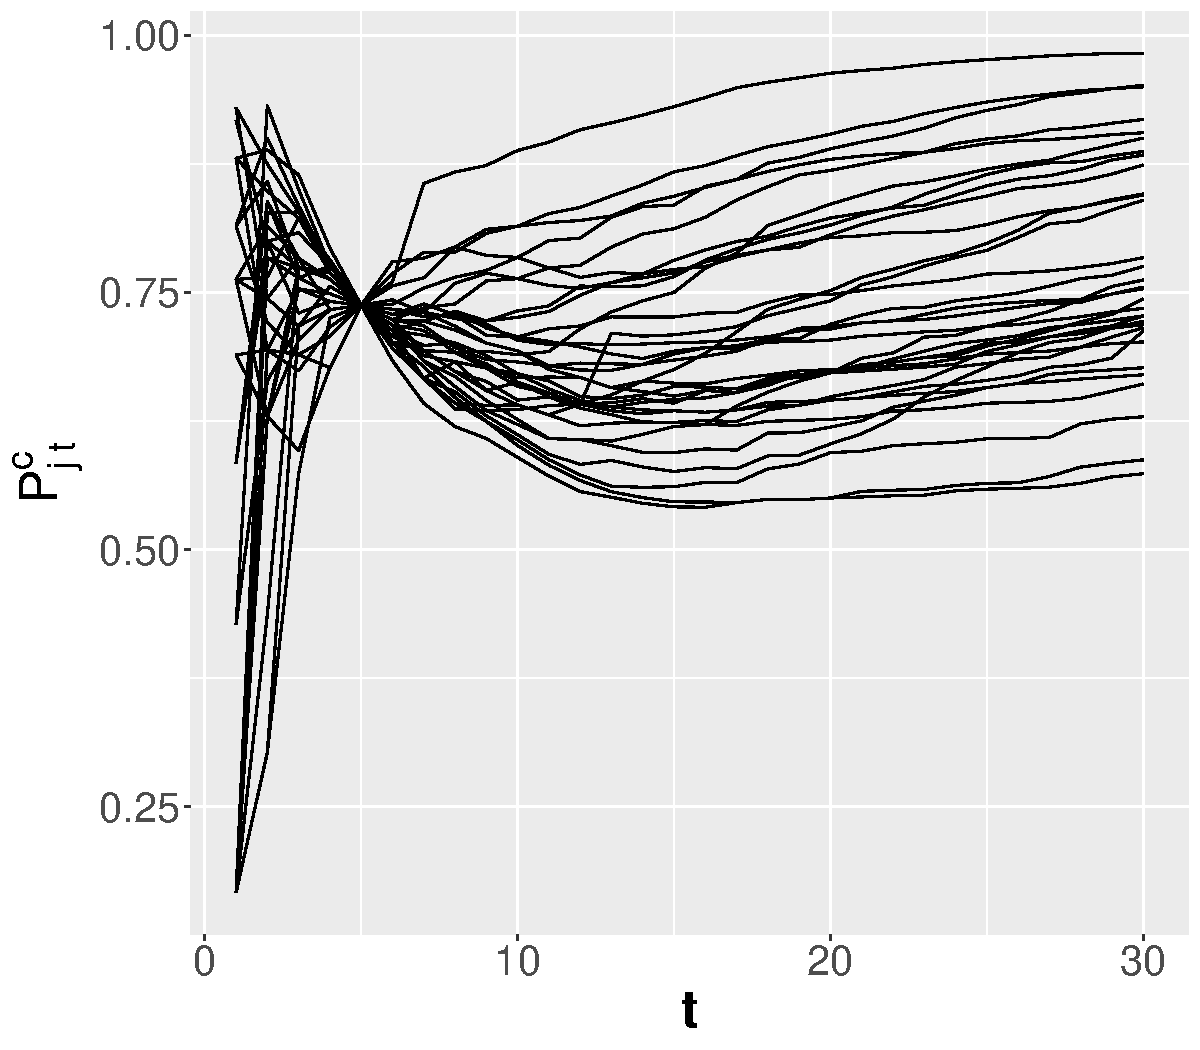
\includegraphics[width=\textwidth]{figures/pred_power/ncit_vs_pubrp/rp_age.pdf}
         \caption{}
         \label{fig:pred_rp_age}
     \end{subfigure}
     \hfill
     \begin{subfigure}[b]{0.48\textwidth}
         \centering
         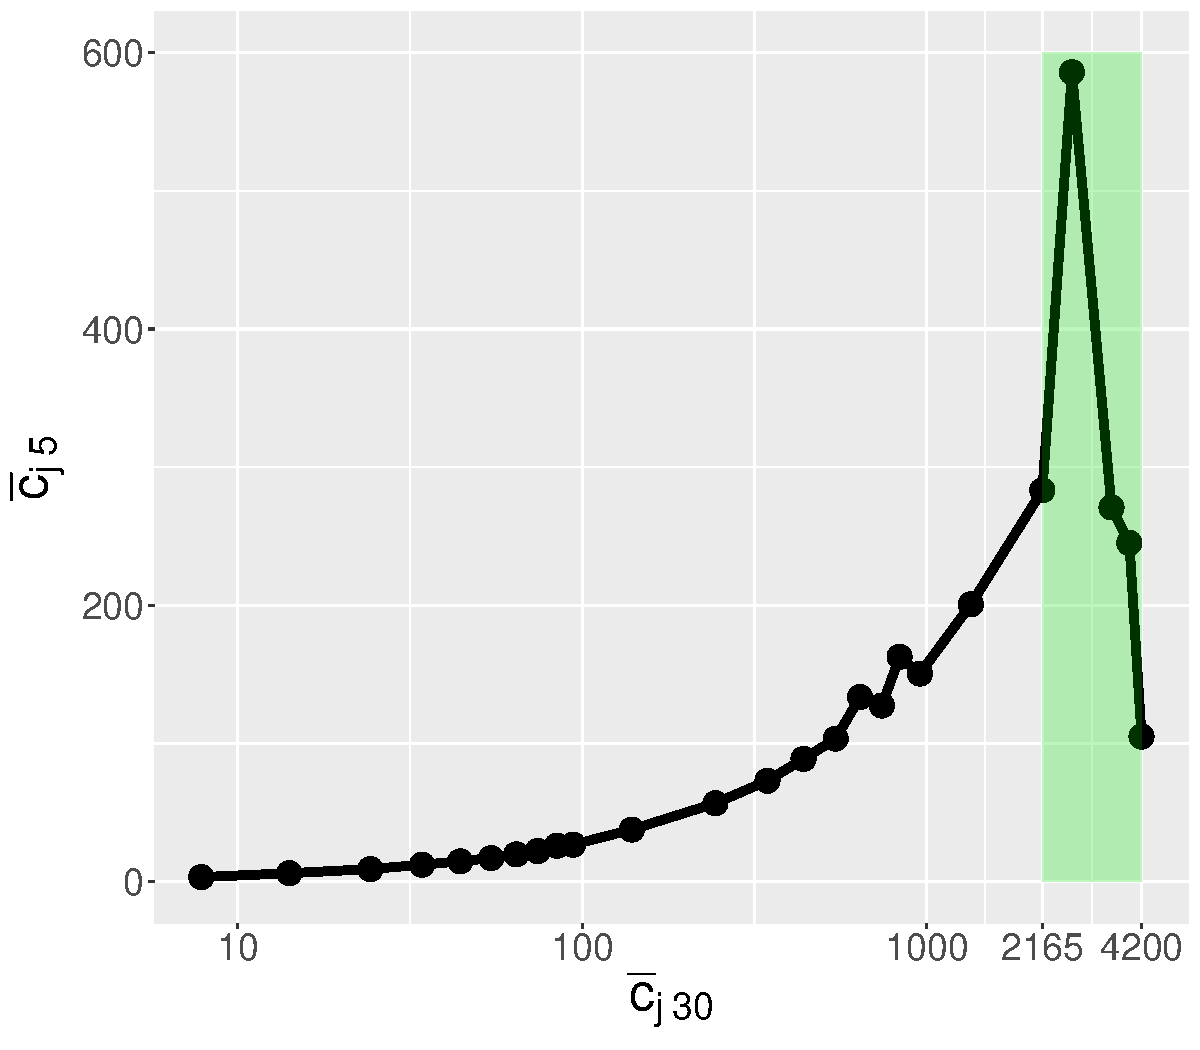
\includegraphics[width=\textwidth]{figures/pred_power/ncit_vs_pubrp/cit_cit.pdf}
         \caption{}
         \label{fig:pred_cit_cit}
     \end{subfigure}
     \hfill
     \begin{subfigure}[b]{0.48\textwidth}
         \centering
         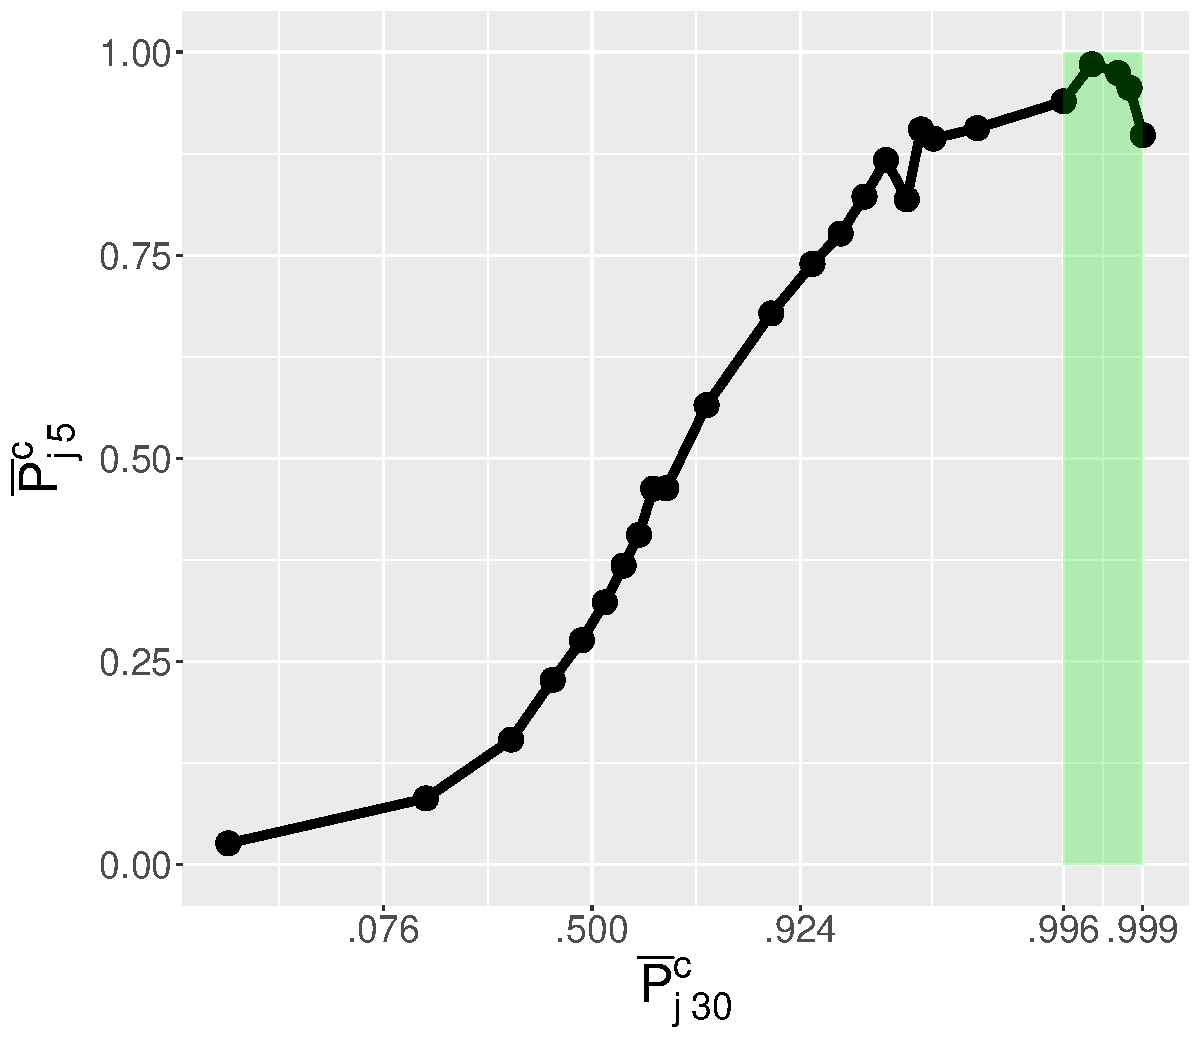
\includegraphics[width=\textwidth]{figures/pred_power/ncit_vs_pubrp/rp_rp.pdf}
         \caption{}
         \label{fig:pred_rp_rp}
     \end{subfigure}
        \caption{The predictability of citations and rank percentiles. The benchmark here is biology. Figure \ref{fig:pred_cit_age} and \ref{fig:pred_rp_age} show the cumulative citations and the corresponding rank percentiles for papers that have $50$ citations by age $5$. Figure \ref{fig:pred_cit_cit} displays the average citations by age $5$ over the average citations by age $30$, for sets of publications, which are pre-specified by dividing the range of $\overline{c_{j 30}}$ into equal intervals in the log scale. Figure \ref{fig:pred_rp_rp} shows the corresponding average rank percentiles for the same sets of publications. Note that we do not claim originality for these plots, as figures \ref{fig:pred_cit_age} and \ref{fig:pred_cit_cit} have been illustrated via a different dataset\supercite{Wang2013}.}
        \label{fig:pub_cit_rp_pred}
\end{figure}


% publication rank percentile, heat map of correlations
\begin{figure}[ht!]
    \centering
    \begin{subfigure}[b]{0.8\textwidth}
        \centering
             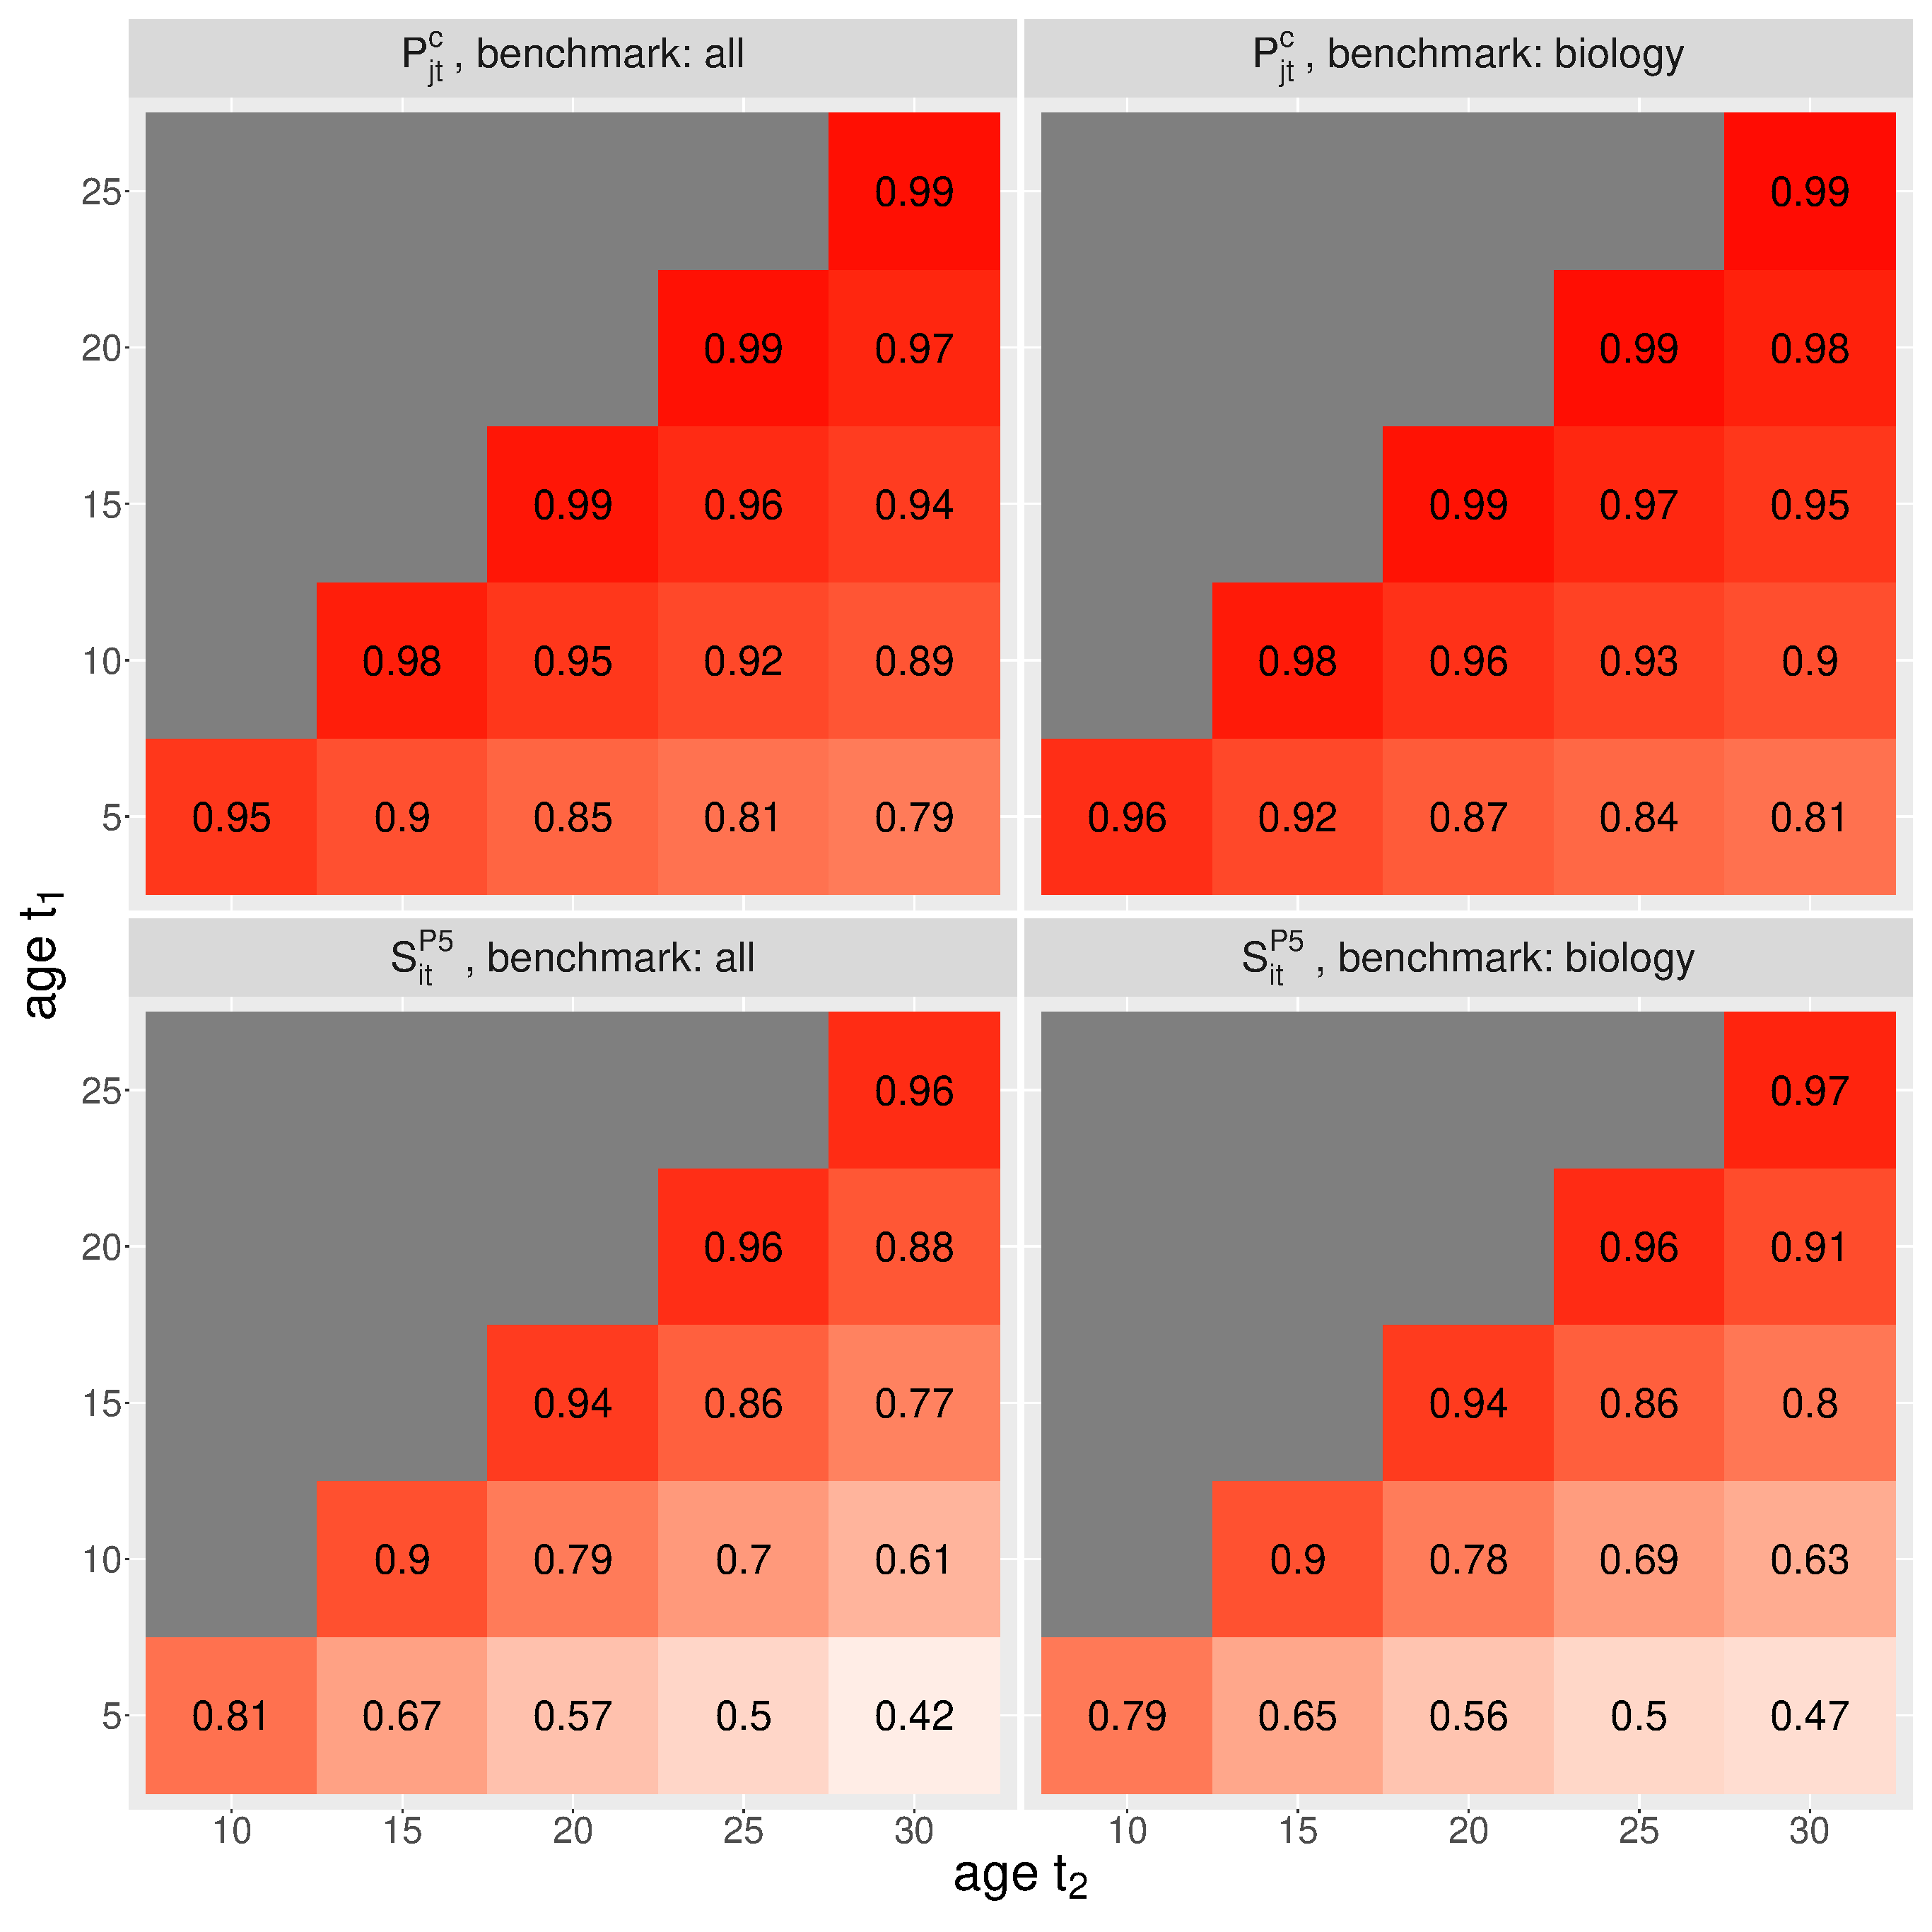
\includegraphics[width=\textwidth]{figures/pred_power/current/heatmap_cor.eps}
         \caption{Predict the cumulative impacts}
         \label{fig:hm_rp_current}
    \end{subfigure}
    
    \begin{subfigure}[b]{0.8\textwidth}
        \centering
             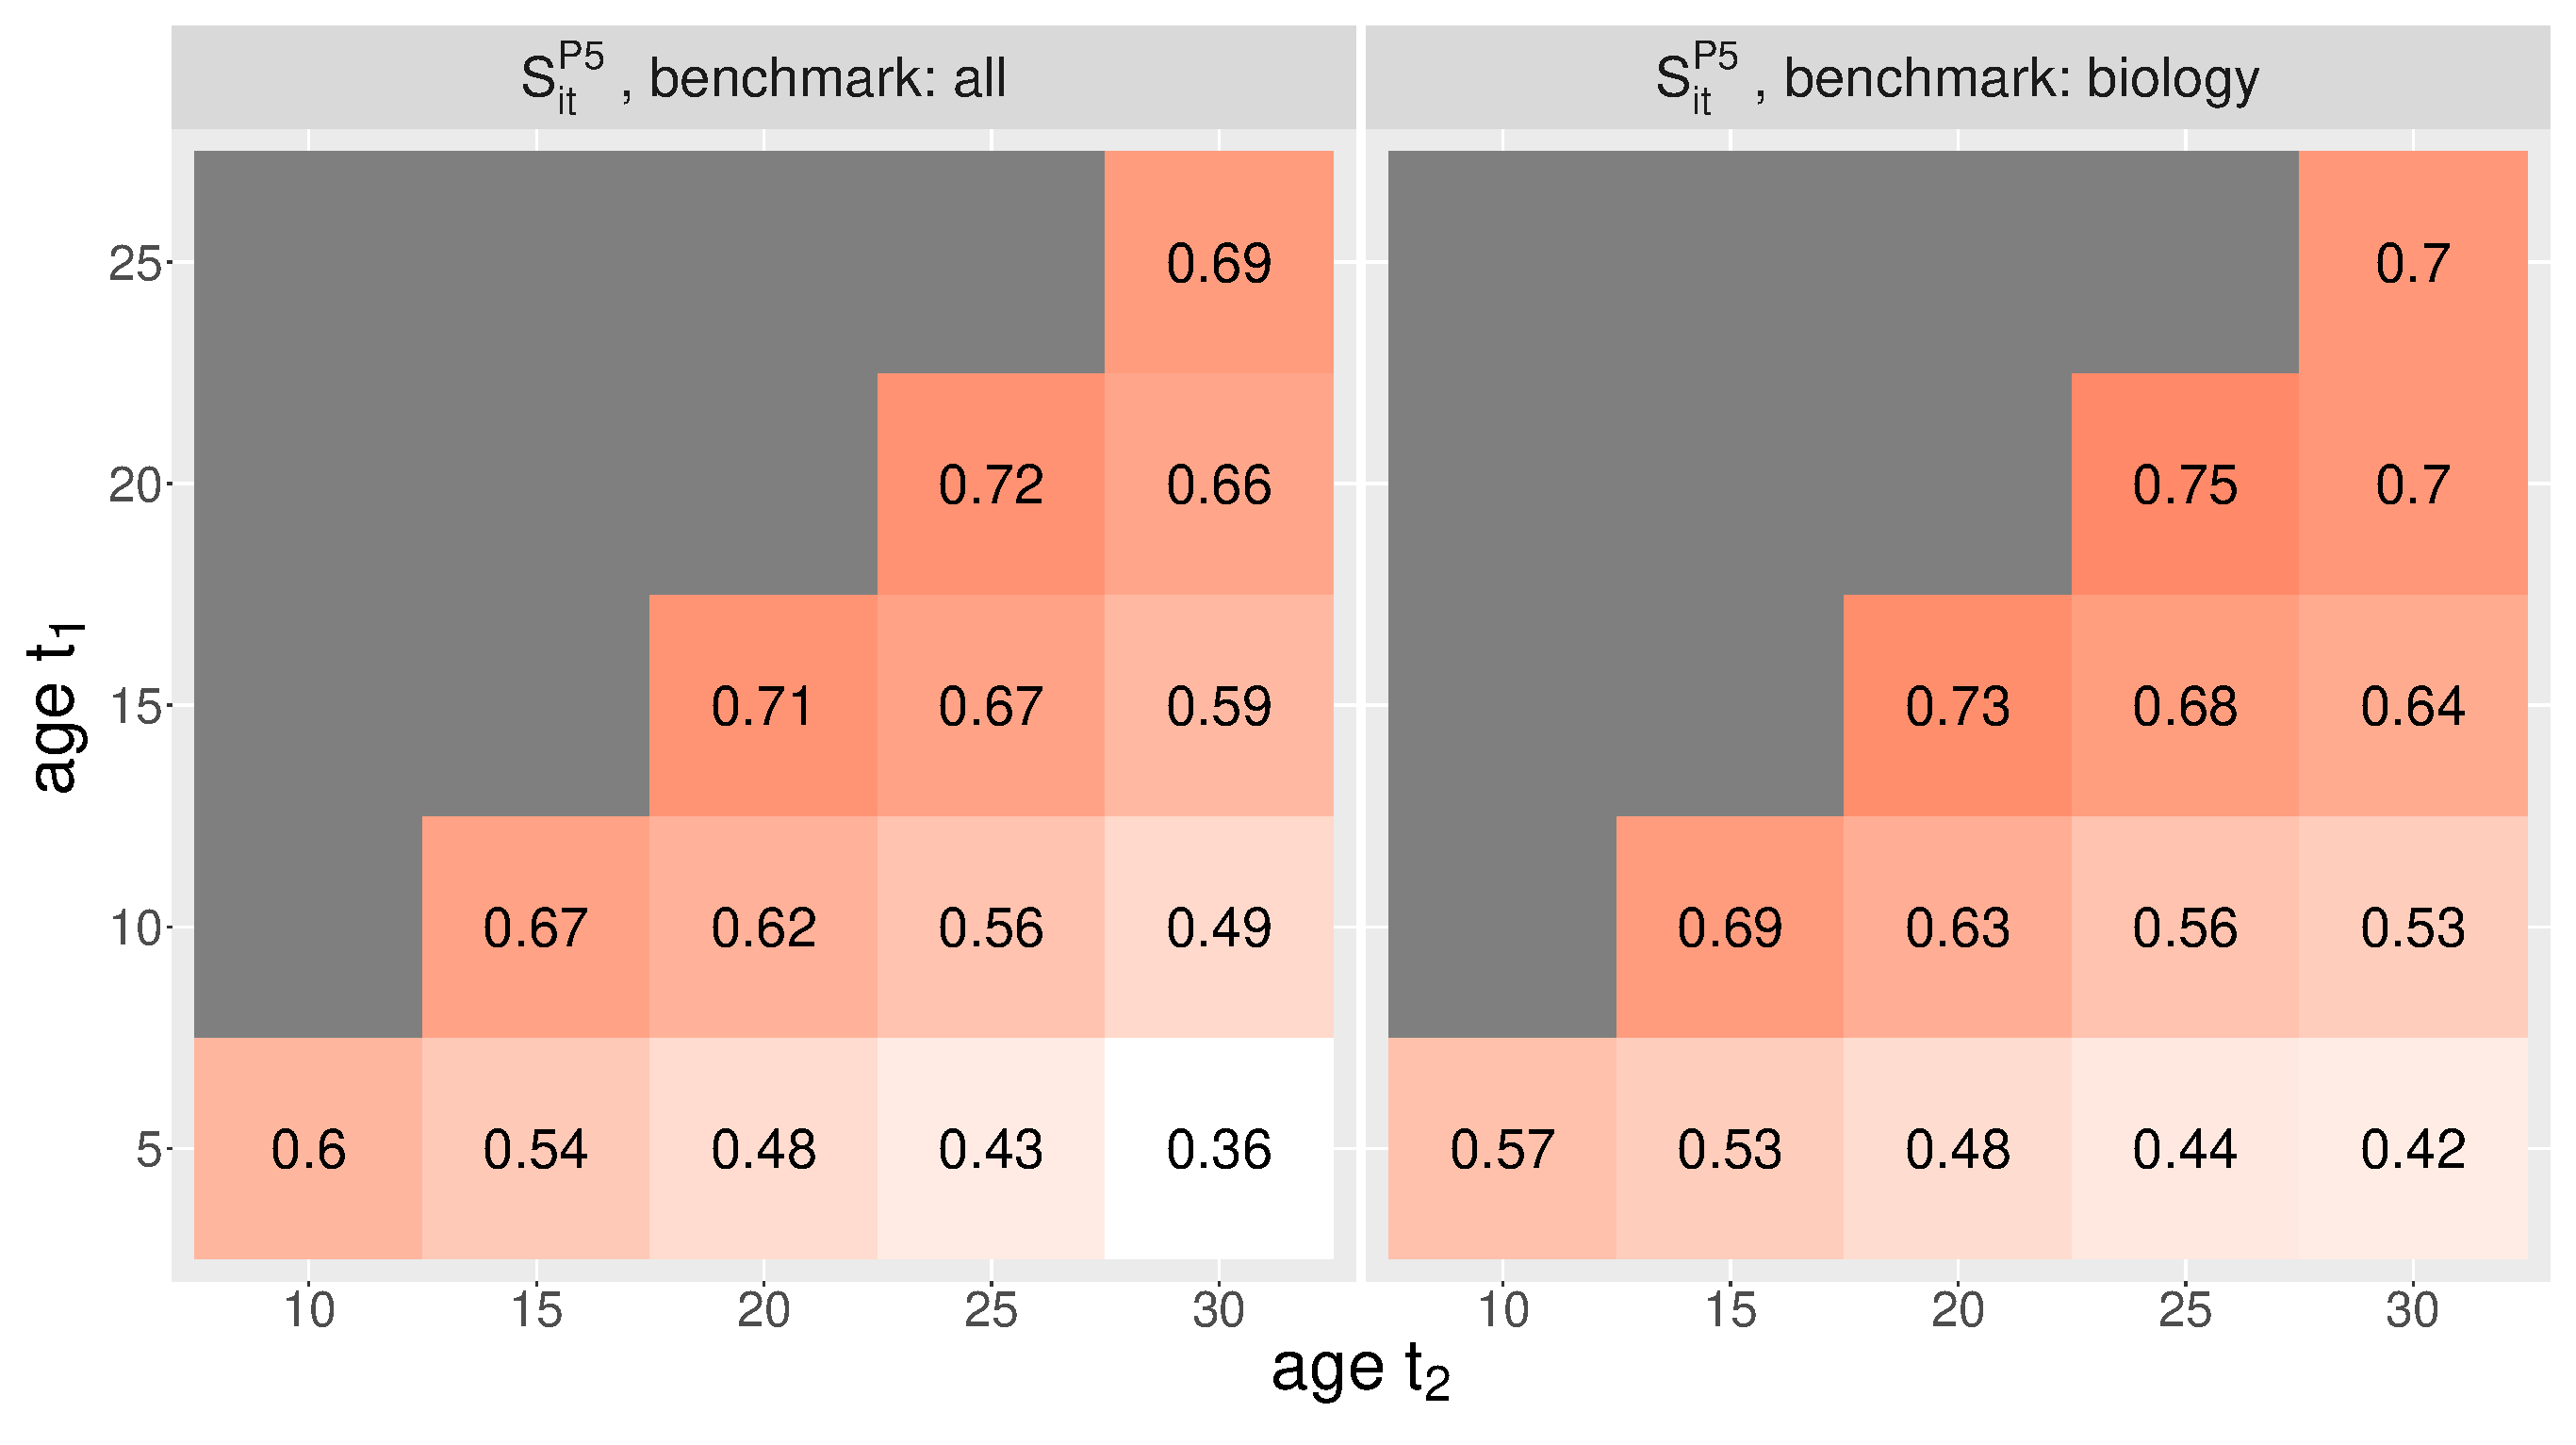
\includegraphics[width=\textwidth]{figures/pred_power/future/heatmap_cor.eps}
         \caption{Predict the future scientific output}
         \label{fig:hm_rp_future}
    \end{subfigure}
    \caption{The Pearson's correlation between rp indicators at two different ages. }
    \label{fig:hm_rp}
\end{figure}
\begin{figure}[ht!]
    \centering
    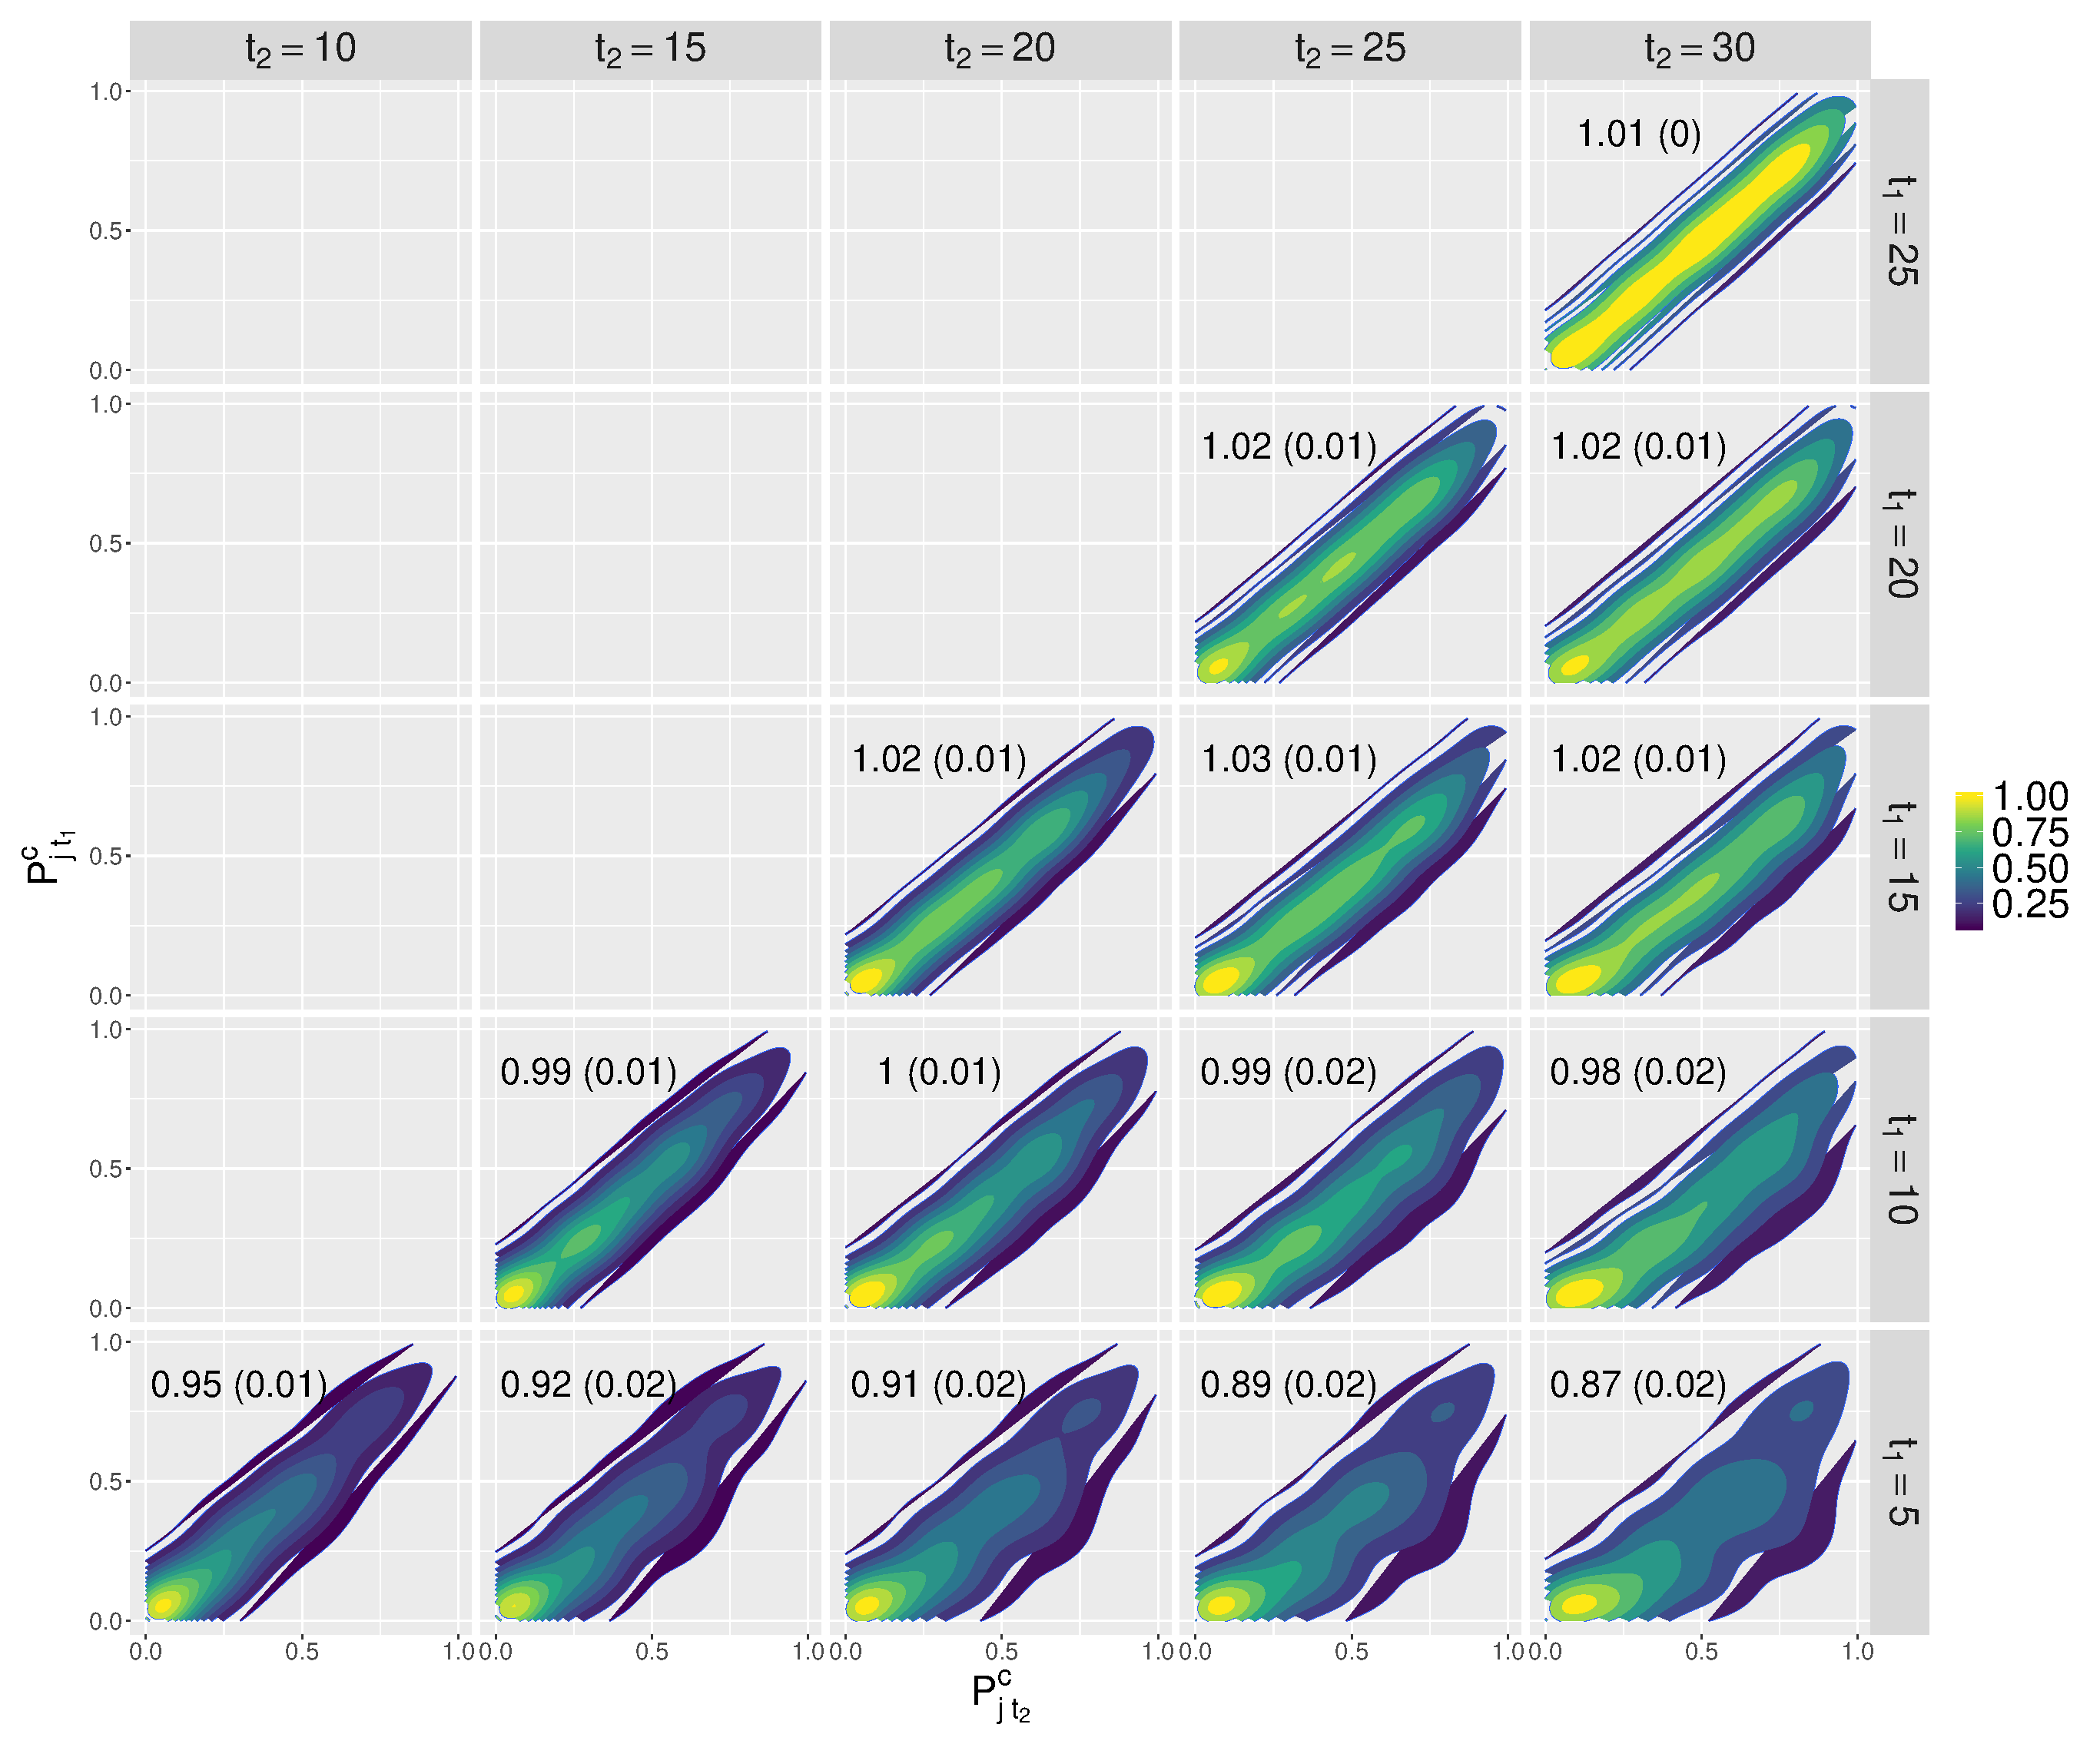
\includegraphics[width=\textwidth]{figures/pred_power/pubrp/scatter_bio1980.eps}
    \caption{Kernel density estimation of the scatters of rp.c$_{\cdot \tau_1}$ and rp.c$_{\cdot \tau_2}$. Meanwhile, we fit a simple linear regression of rp.c$_{\cdot \tau_2}$ upon rp.c$_{\cdot \tau_1}$. The estimated coefficient of rp.c$_{\cdot \tau_1}$ and the corresponding standard error (in the bracket) are displayed in each facet. The benchmark here includes all publications in biology and written in $1980$.}
    \label{fig:scatter_pubrp_bio1980}
\end{figure}

\iffalse
% author rank percentile, heat map of correlations
\begin{figure}[ht!]
    \centering
    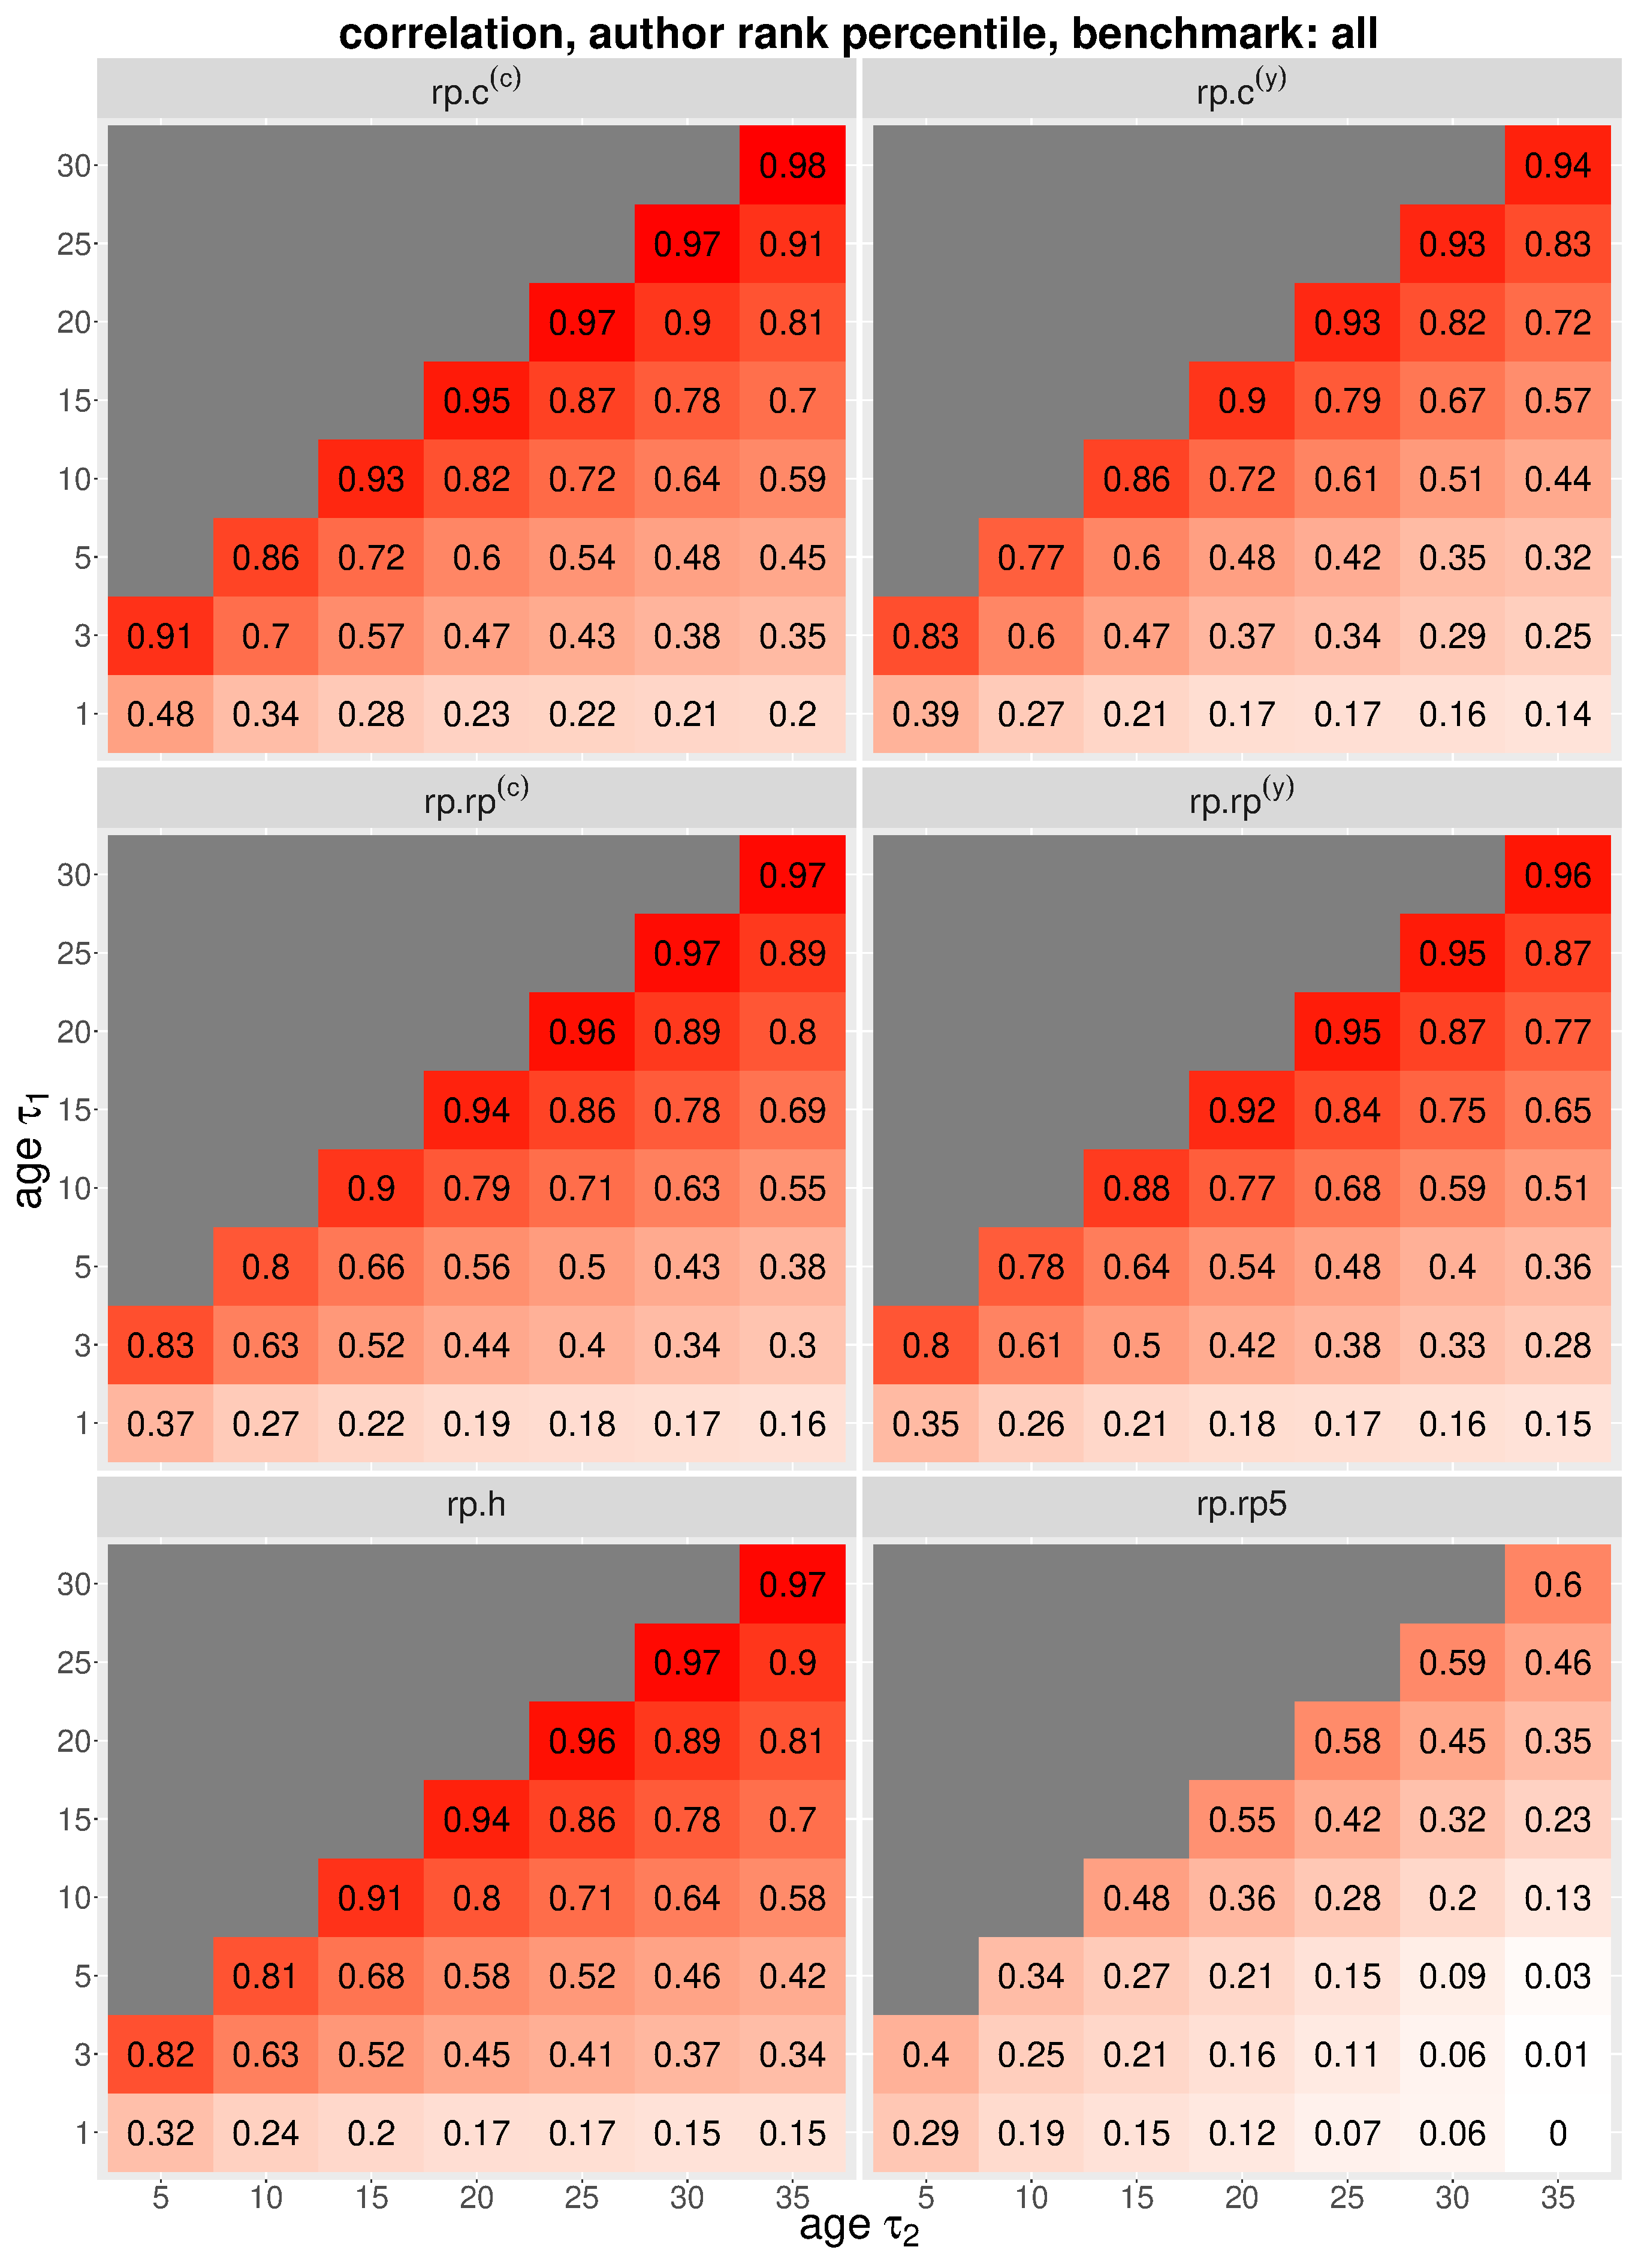
\includegraphics[width=\textwidth]{figures/pred_power/autrp/heatmap_cor_all.eps}
    \caption{The Pearson's correlation between rp at two different ages, for various types of author rp. The benchmark includes all the authors.}
    \label{fig:hm_autrp_all}
\end{figure}
\begin{figure}[ht!]
    \centering
    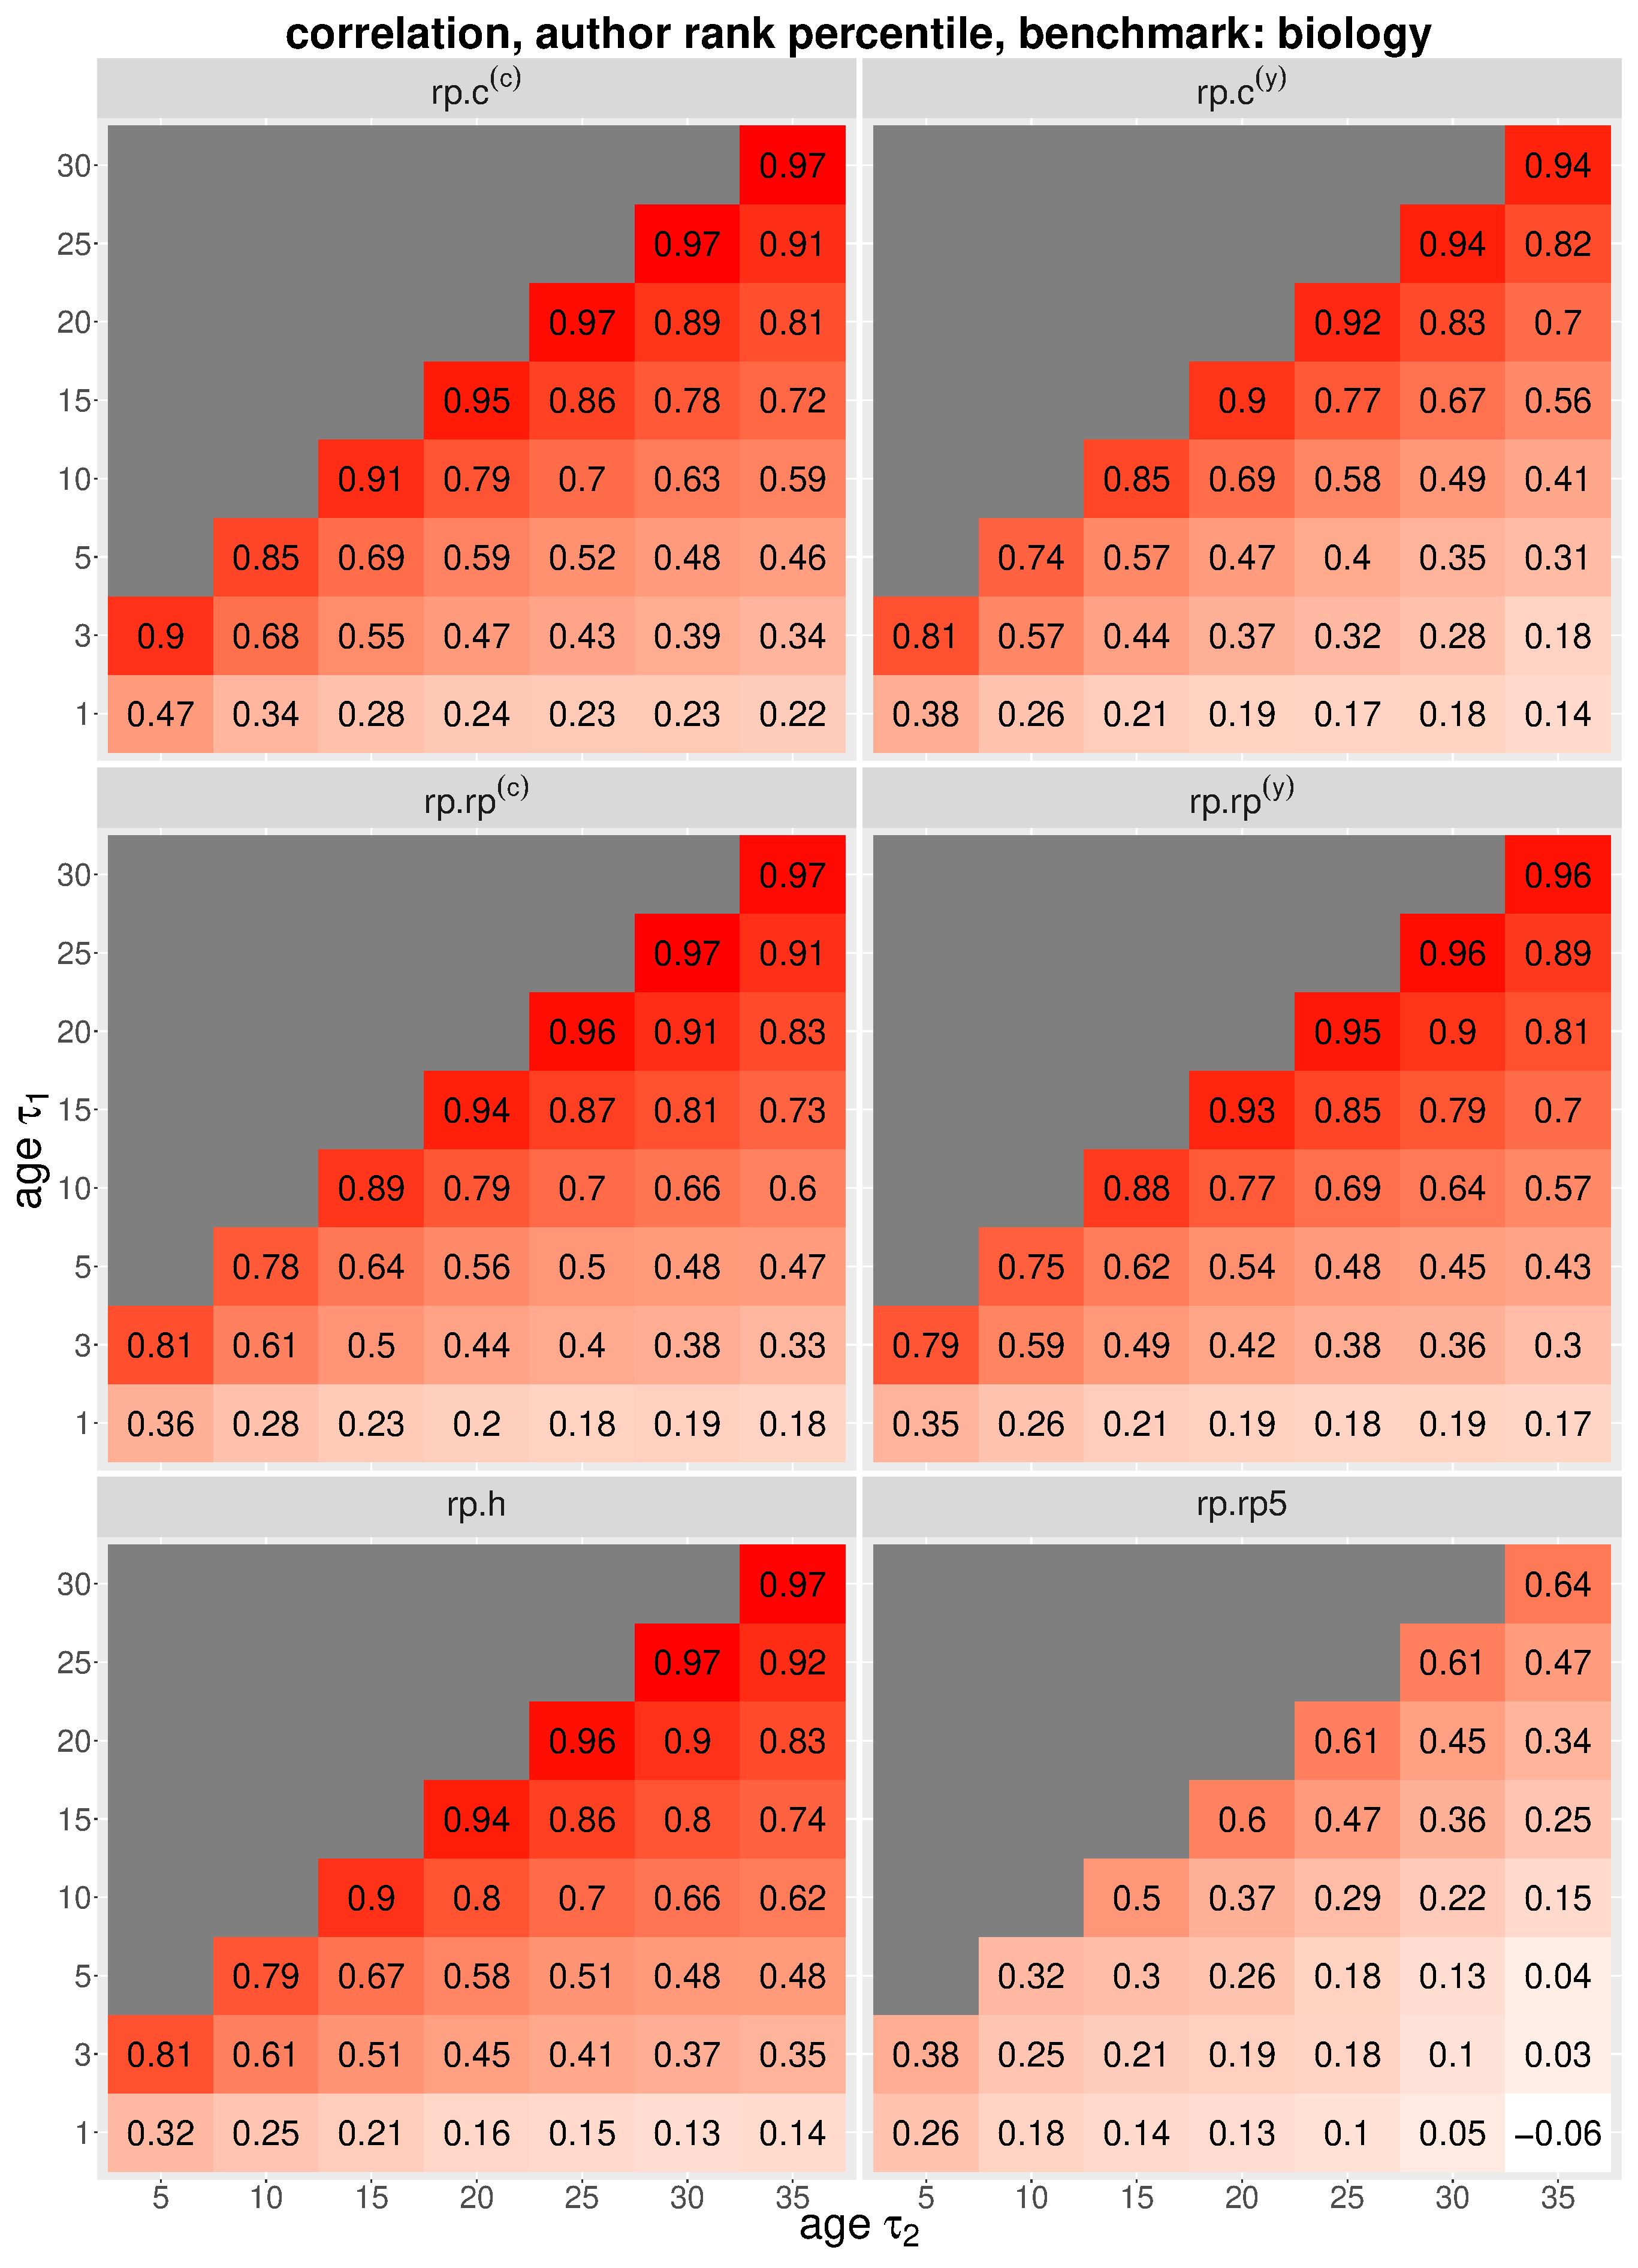
\includegraphics[width=\textwidth]{figures/pred_power/autrp/heatmap_cor_bio.eps}
    \caption{The Pearson's correlation between rp at two different ages, for various types of author rp. The benchmark includes only authors in biology.}
    \label{fig:hm_autrp_biology}
\end{figure}

\begin{figure}[ht!]
    \centering
    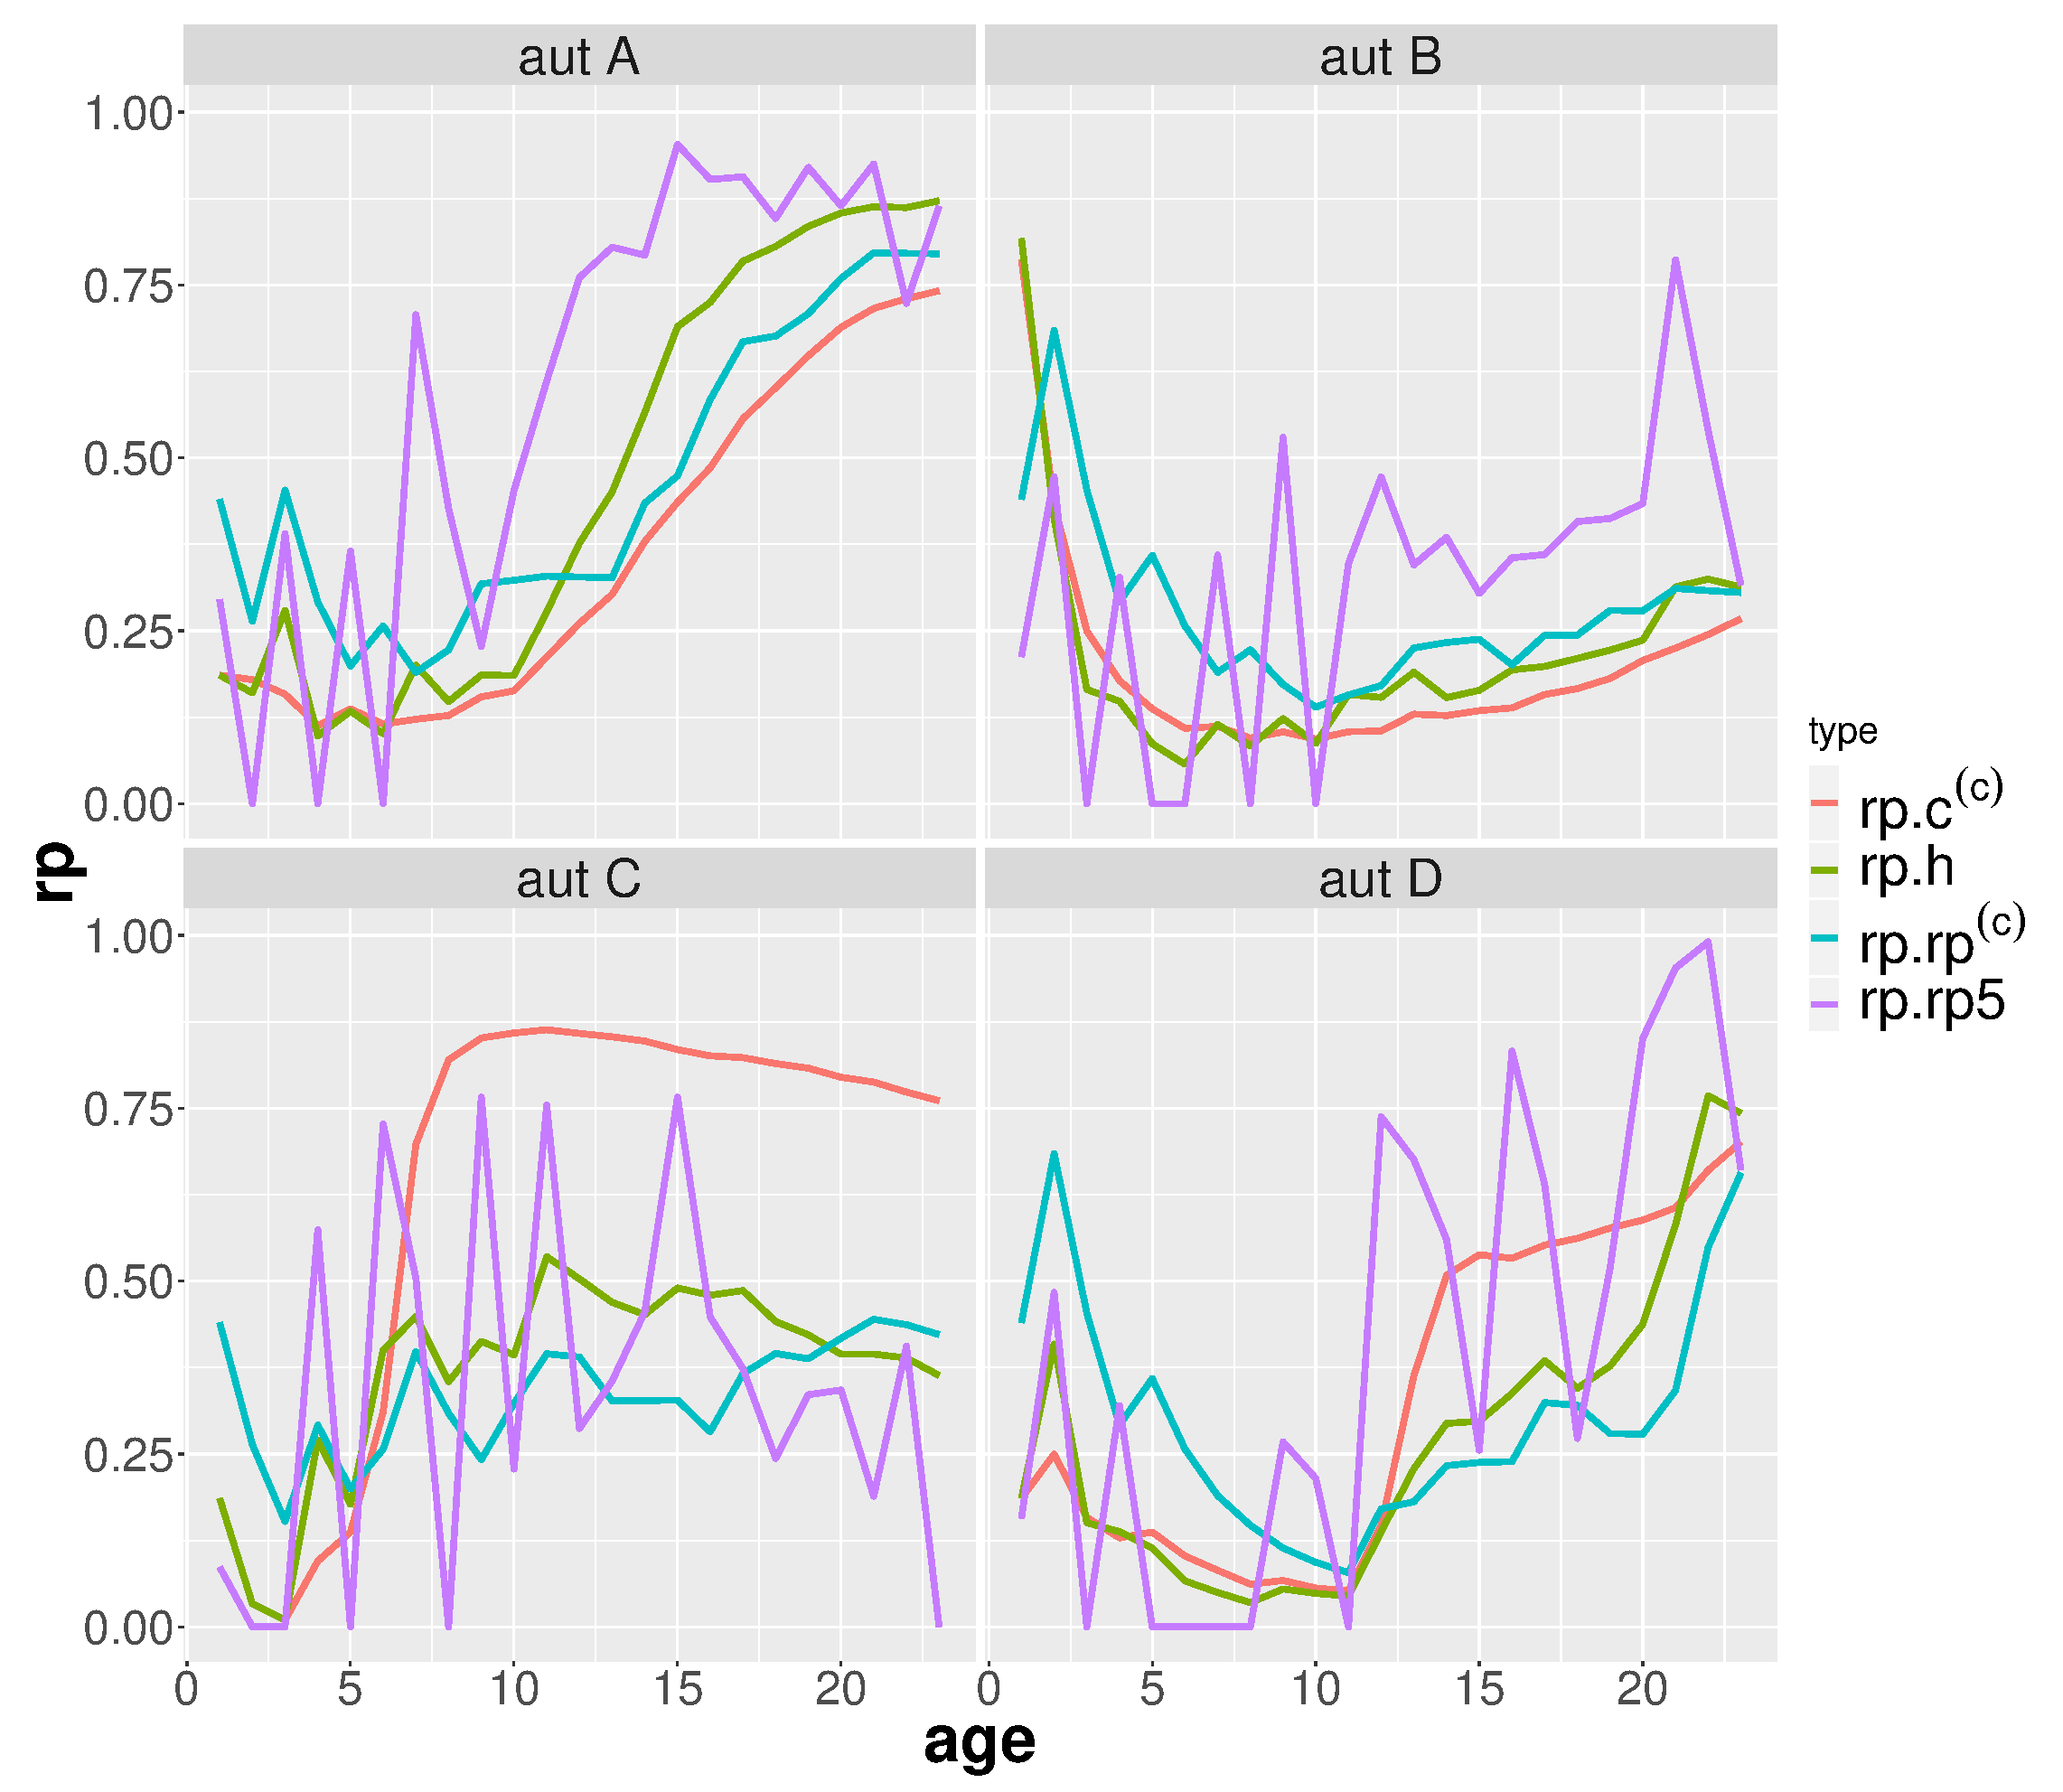
\includegraphics[width=\textwidth]{figures/exploratory/autrp_examples.eps}
    \caption{Examples of various types of author rank percentile over age. The $4$ authors shown in the figure have the same $\text{rp}^{(c)}_{i 5}$ and are all starting their careers from year $1990$. }
    \label{fig:aut_examples}
\end{figure}
\fi

\begin{figure}[ht!]
    \centering
    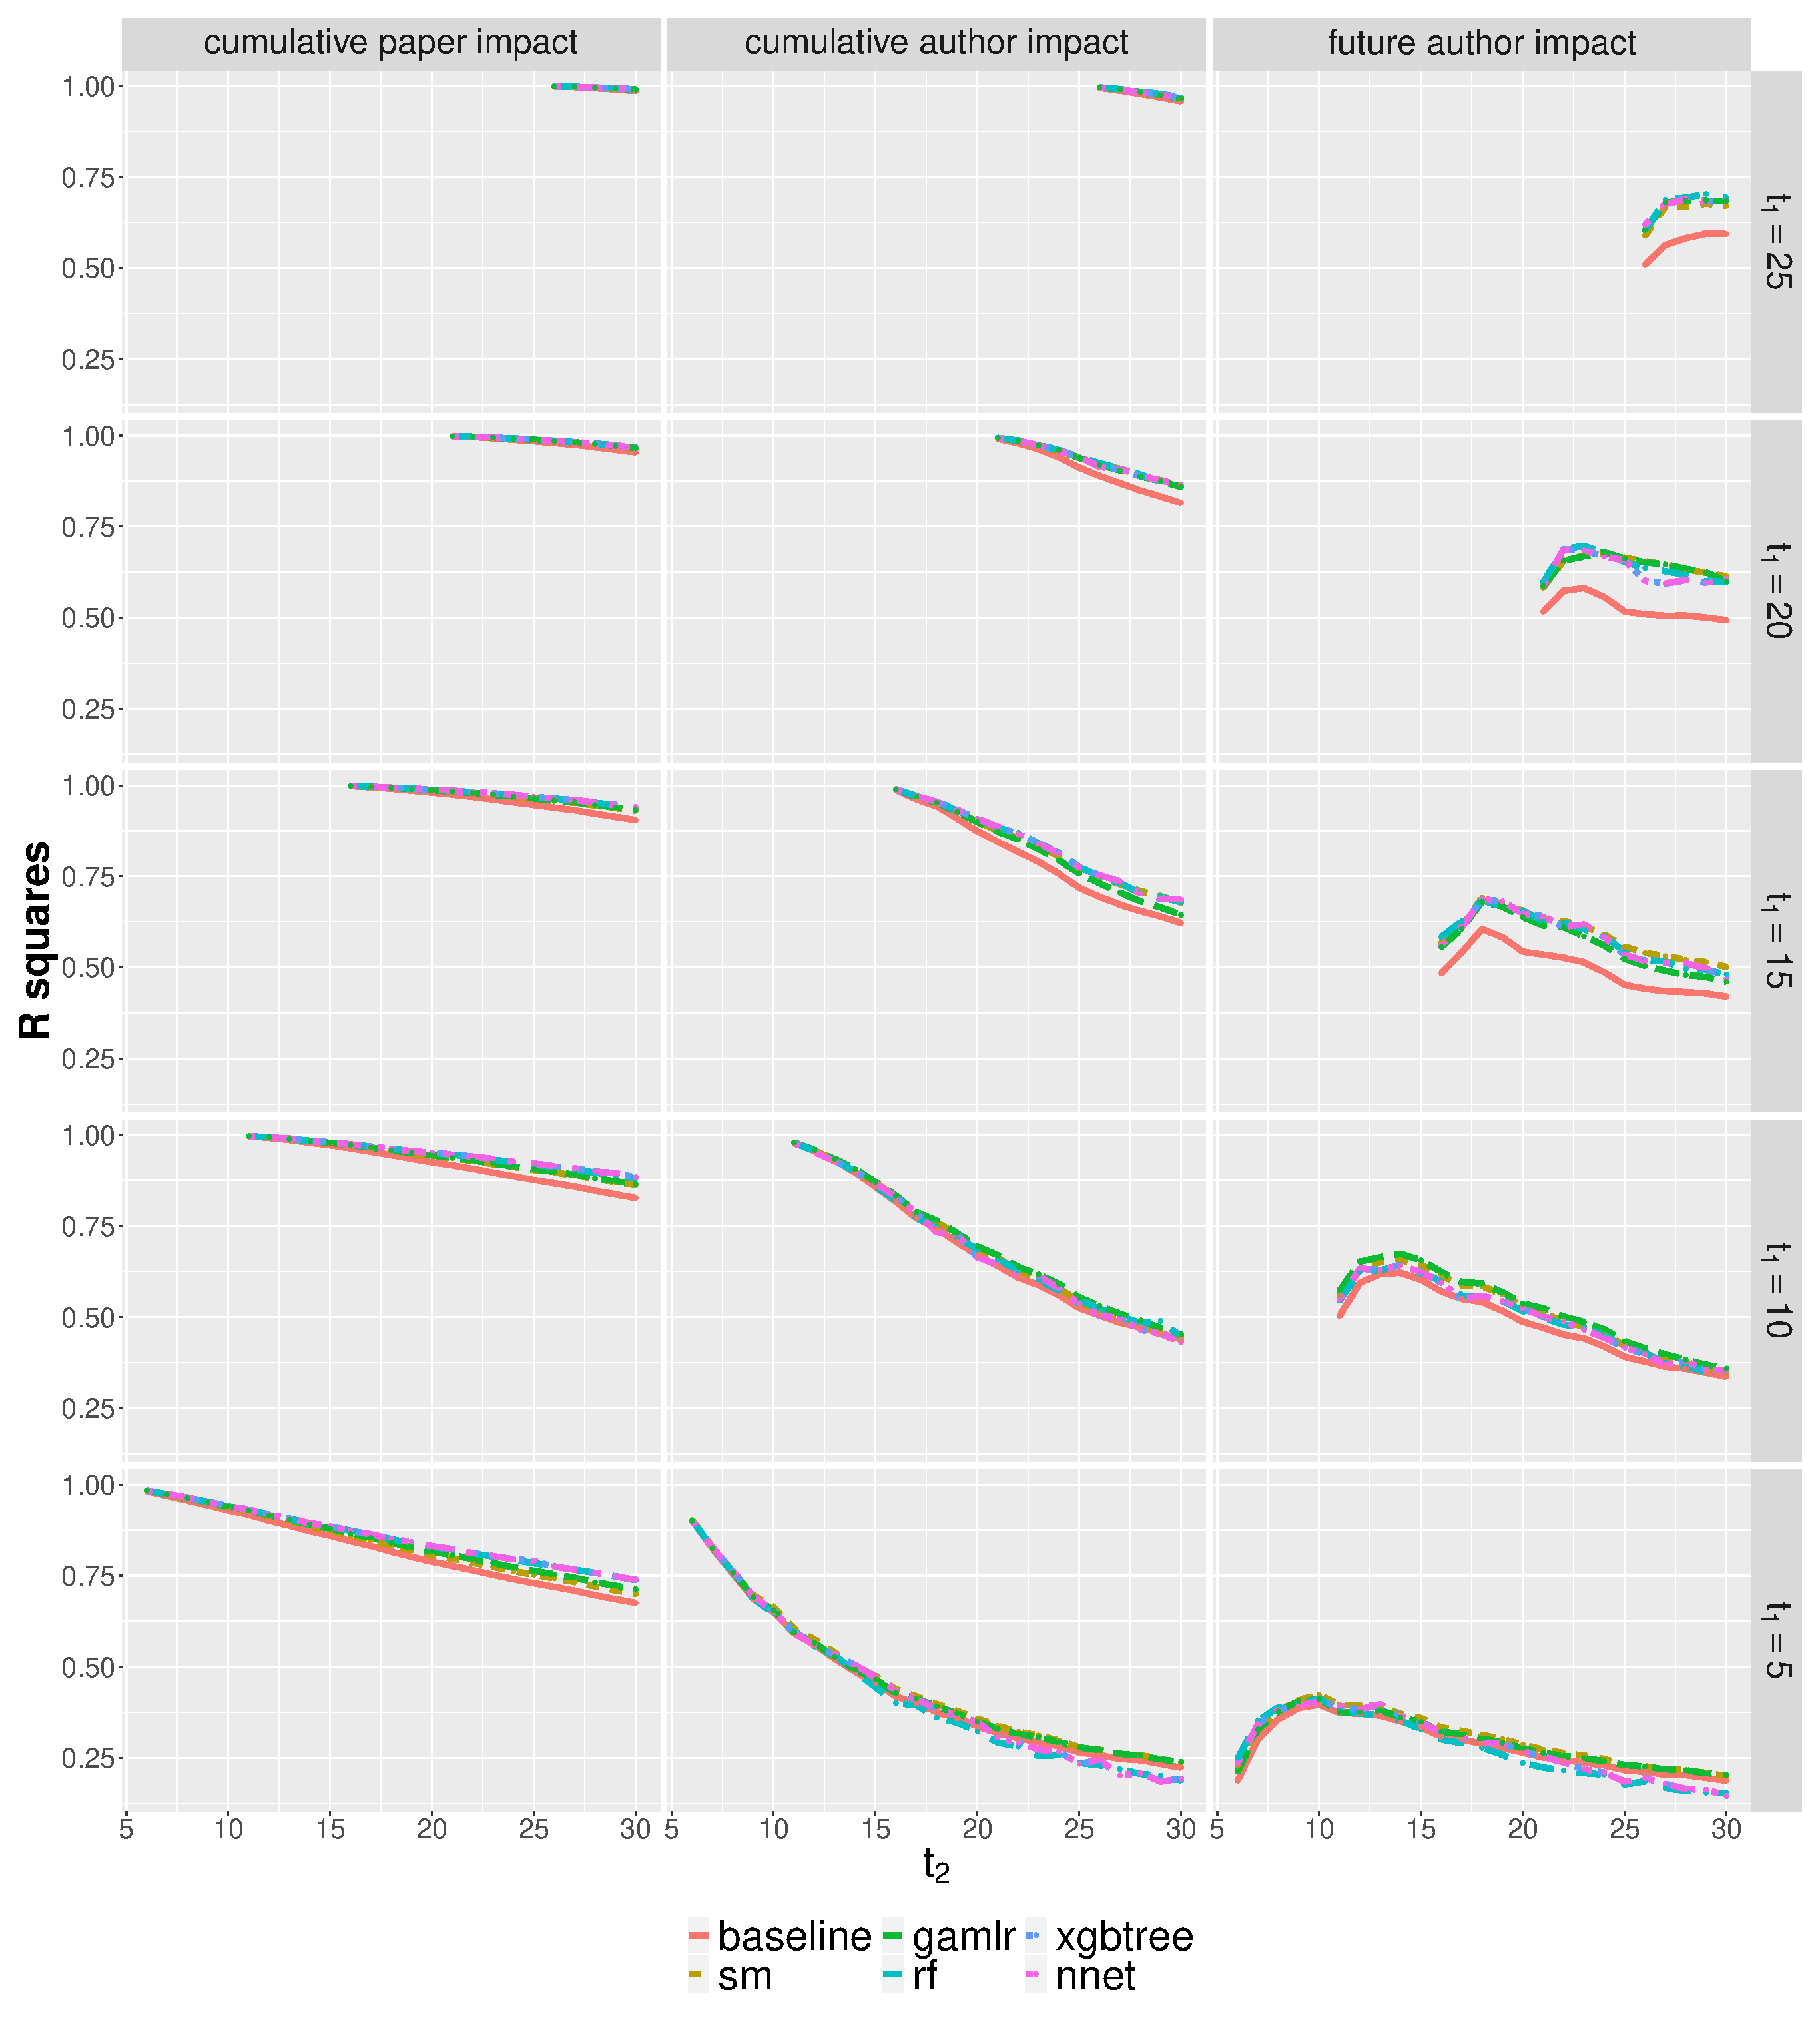
\includegraphics[width=\textwidth]{figures/pred_model/r2_diff.eps}
    \caption{Testing R squares of the predictive models. LASSO, ridge and elastic net are outperformed by Gamma LASSO, and hence are ignored for a better visualization.}
    \label{fig:pred_r2}
\end{figure}


\iffalse
\begin{figure}[ht!]
    \centering
        \begin{subfigure}[t]{0.8\textwidth}
        \centering
        \includegraphics[width=\textwidth]{figures/pred_model/pub/bio/importance.pdf}
        \caption{Top 5 features for predicting publication rp}
    \end{subfigure}%
    
    \begin{subfigure}[t]{0.8\textwidth}
        \centering
        \includegraphics[width=\textwidth]{figures/pred_model/aut/all/importance.pdf}
        \caption{Top 5 features for predicting author rp}
    \end{subfigure}

    \caption{Random permutation importance of features for predicting rank percentiles given by the random forest models. The top 5 features are selected based on the median of their importance values. }
    \label{fig:pred_model_importance}
\end{figure}
\fi



%!TEX root = ms.tex
\clearpage
\begin{refsection}
%\renewcommand*{\thepage}{A\arabic{page}}
\beginsupplement
\appendix
\pagenumbering{arabic}
\begin{center}
\textbf{\large Supplemental Material: \\ On the Predictability of Utilizing Rank Percentile to Evaluate Scientific Impact}

Sen Tian, Panos Ipeirotis
\end{center}

\section{Rank Percentile Indicators for Scholars}
\label{sec:suppl_similarity_autrp}

We consider the benchmark being the field of biology. In order to study the agreement of various indicators, for each indicator, we classify the scholars into four classes, class $1$: $0\le \text{S}_m^{i}(t) < 0.25$, class $2$: $0.25\le \text{S}_m^{i}(t) < 0.5$, class $3$: $0.5 \le \text{S}_m^{i}(t) < 0.75$ and class $4$: $0.75 \le \text{S}_m^{i}(t) \le 1$. An agreement is when two (or three) different indicators belong to the same class. The overall agreement for all three indicators, S$_{P5}$, S$_c$, and S$_h$, is $51\%$ at age $5$ and $68\%$ at age $30$; that is, for about half of the scholars the three indicators agree with each other at age $5$, while that number becomes around two third at age $30$. Figure \ref{fig:aut_rp_class} displays pairwise agreement of the three indicators. We see that the agreement increases with the age. Furthermore, S$_{P5}$ has large agreement with both S$_{c}$ and S$_{h}$, which are $69\%$ and $67\%$, respectively, at age $5$, and $71\%$ and $81\%$, respectively, at age $30$. 

Figure \ref{fig:hm_autrp_current} shows the correlation between S$_c^{i}(t_1)$ and S$_c^{i}(t_2)$, and the correlation between S$_h^{i}(t_1)$ and S$_h^{i}(t_2)$. The magnitudes of correlations are similar to those for S$_{P5}$ as shown in Figure \ref{fig:hm_rp_aut}.

% fig:aut_rp_class
% class agreement among all the author rp
\begin{figure}[ht!]
    \centering
    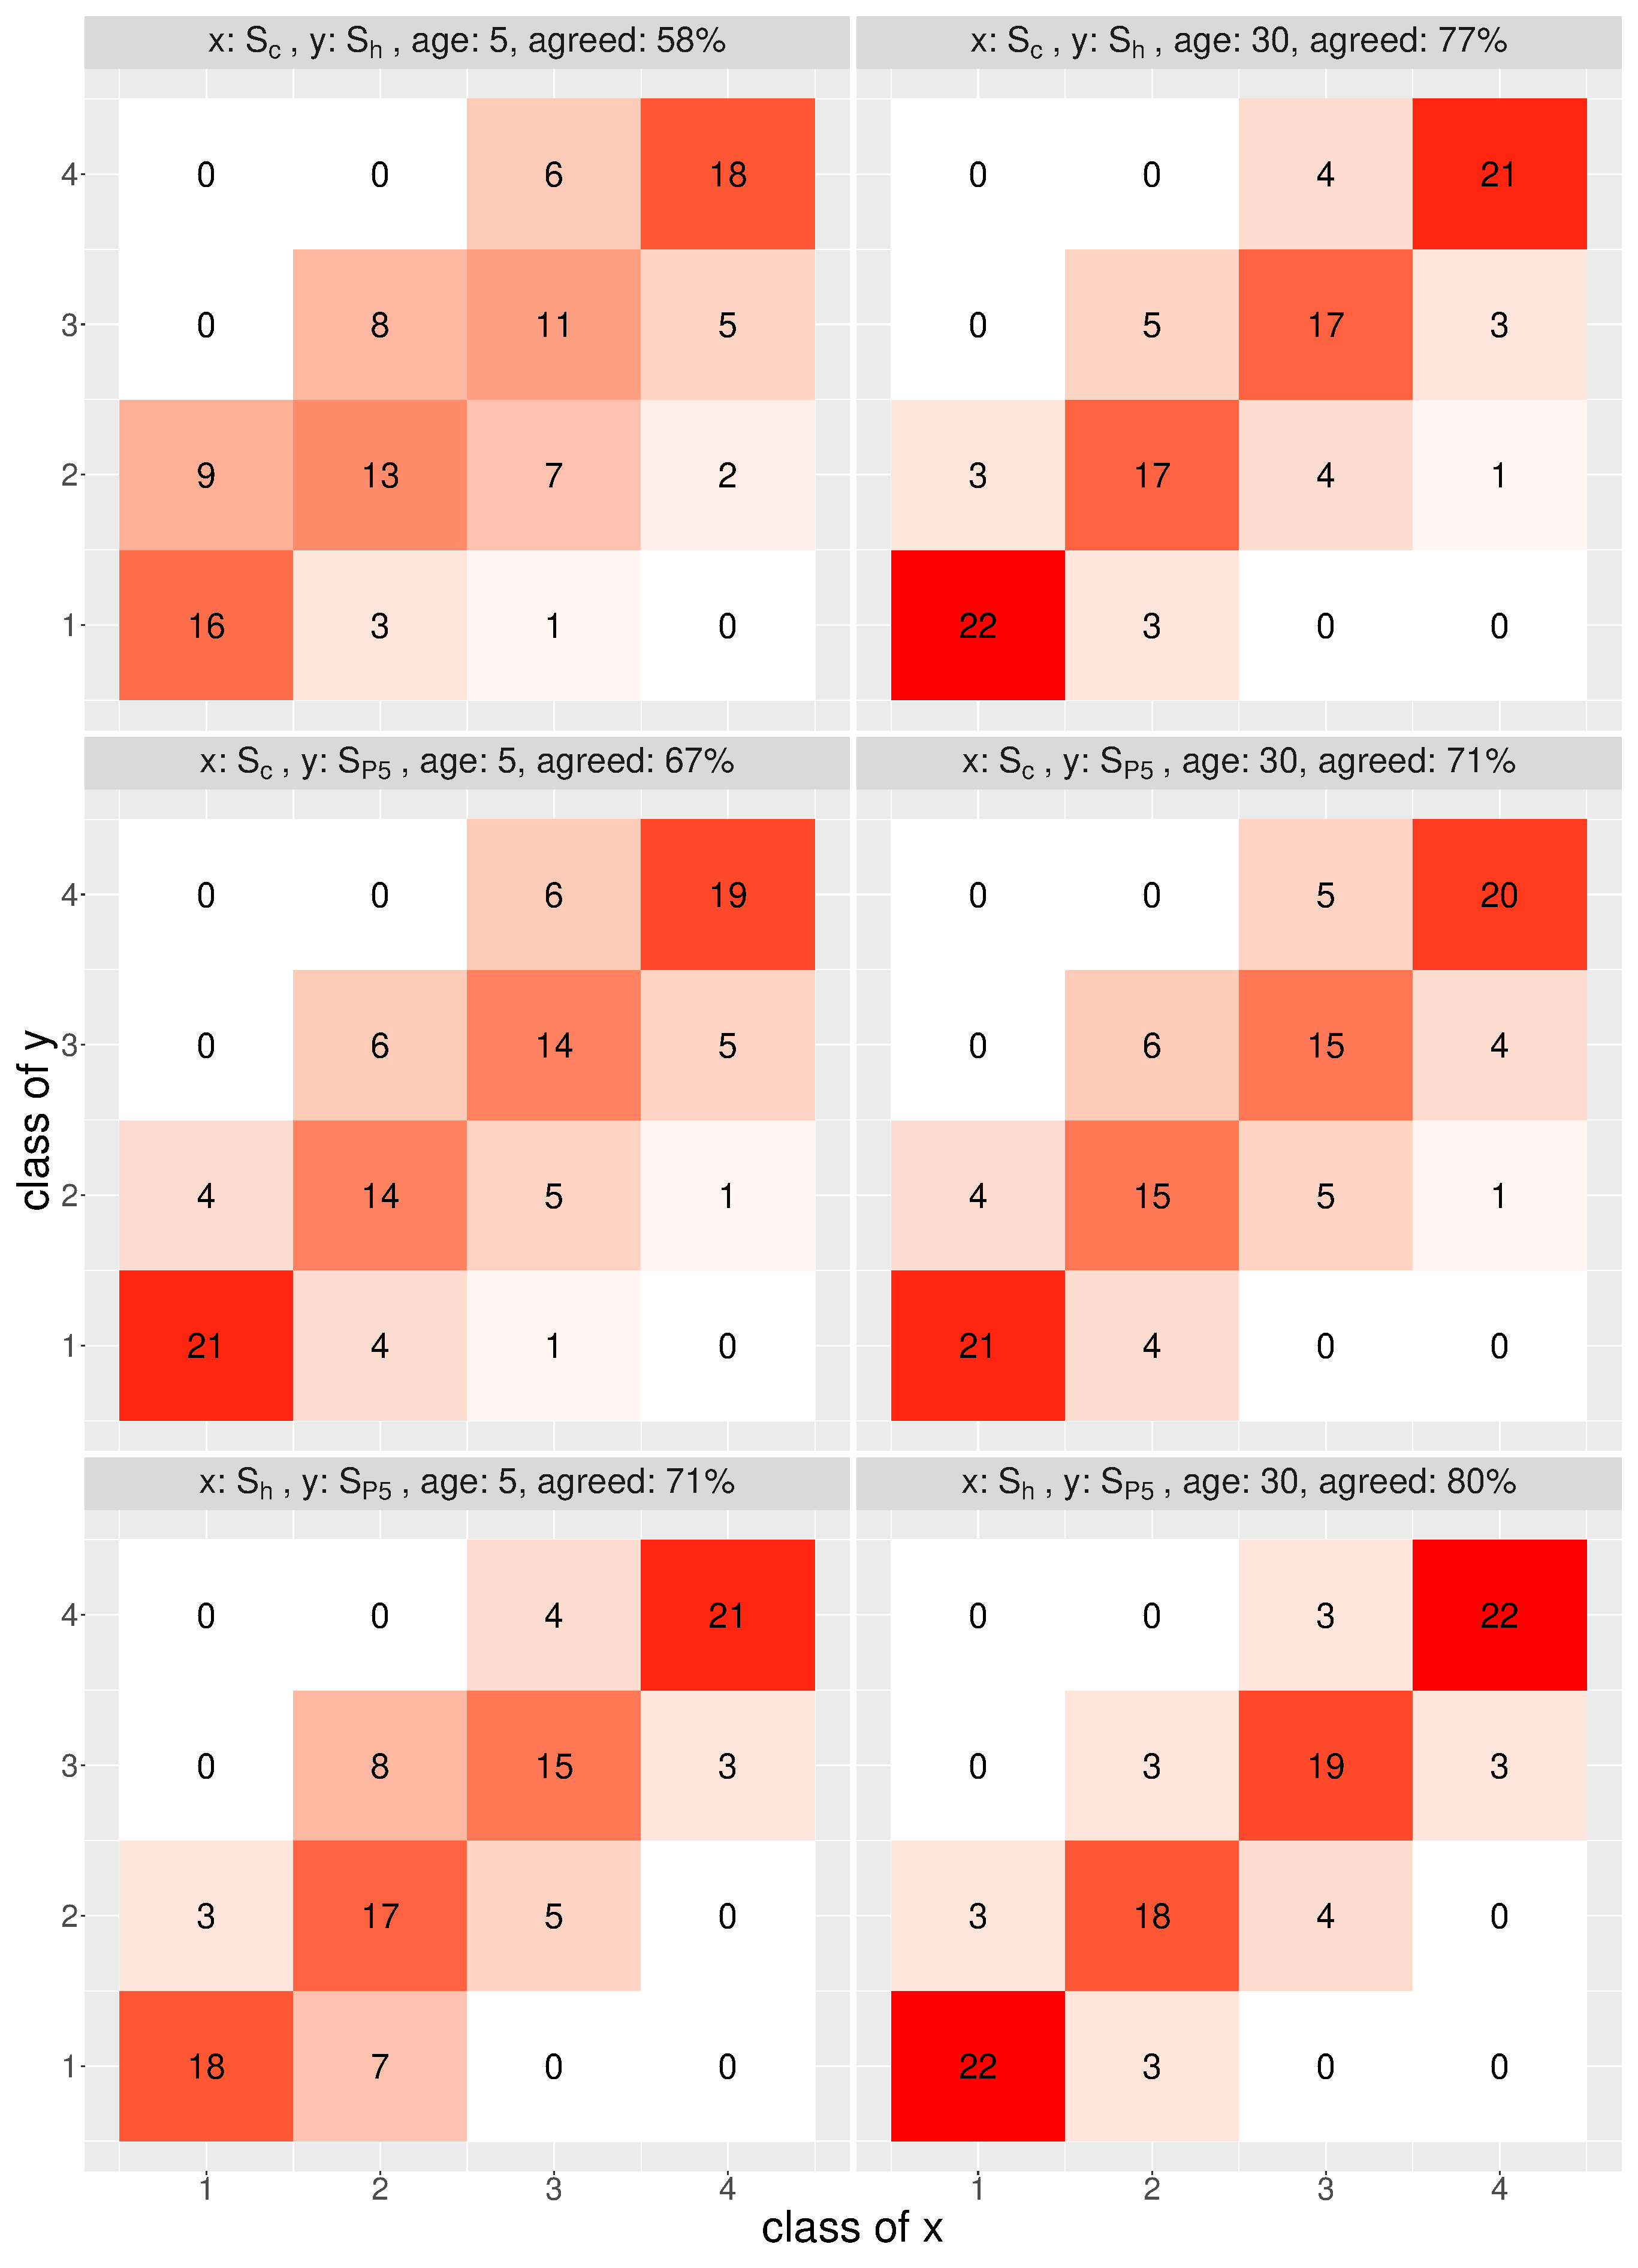
\includegraphics[width=0.88\textwidth]{figures/compare_autrp/heatmap_class_agreement.eps}
    \caption{{\bf The Agreement of Rank Percentile Indicators for Scholars.} 
    Rank percentile indicators are classified into four groups, that are class $1$: $0 \le \text{S}_m^{i}(t) < 0.25$, class $2$: $0.25 \le \text{S}_m^{i}(t) < 0.5$, class $3$: $0.5 \le \text{S}_m^{i}(t) < 0.75$ and class $4$: $0.75 \le \text{S}_m^{i}(t) \le 1$. The agreement of classes (sum of the anti-diagonal elements) is displayed in the title of each panel. The benchmark is biology. The agreement for all three indicators is $51 \%$ at age $5$ and is $68 \%$ at age $30$.}
    \label{fig:aut_rp_class}
\end{figure}

% publication rank percentile, heat map of correlations
\begin{figure}[ht!]
    \centering
    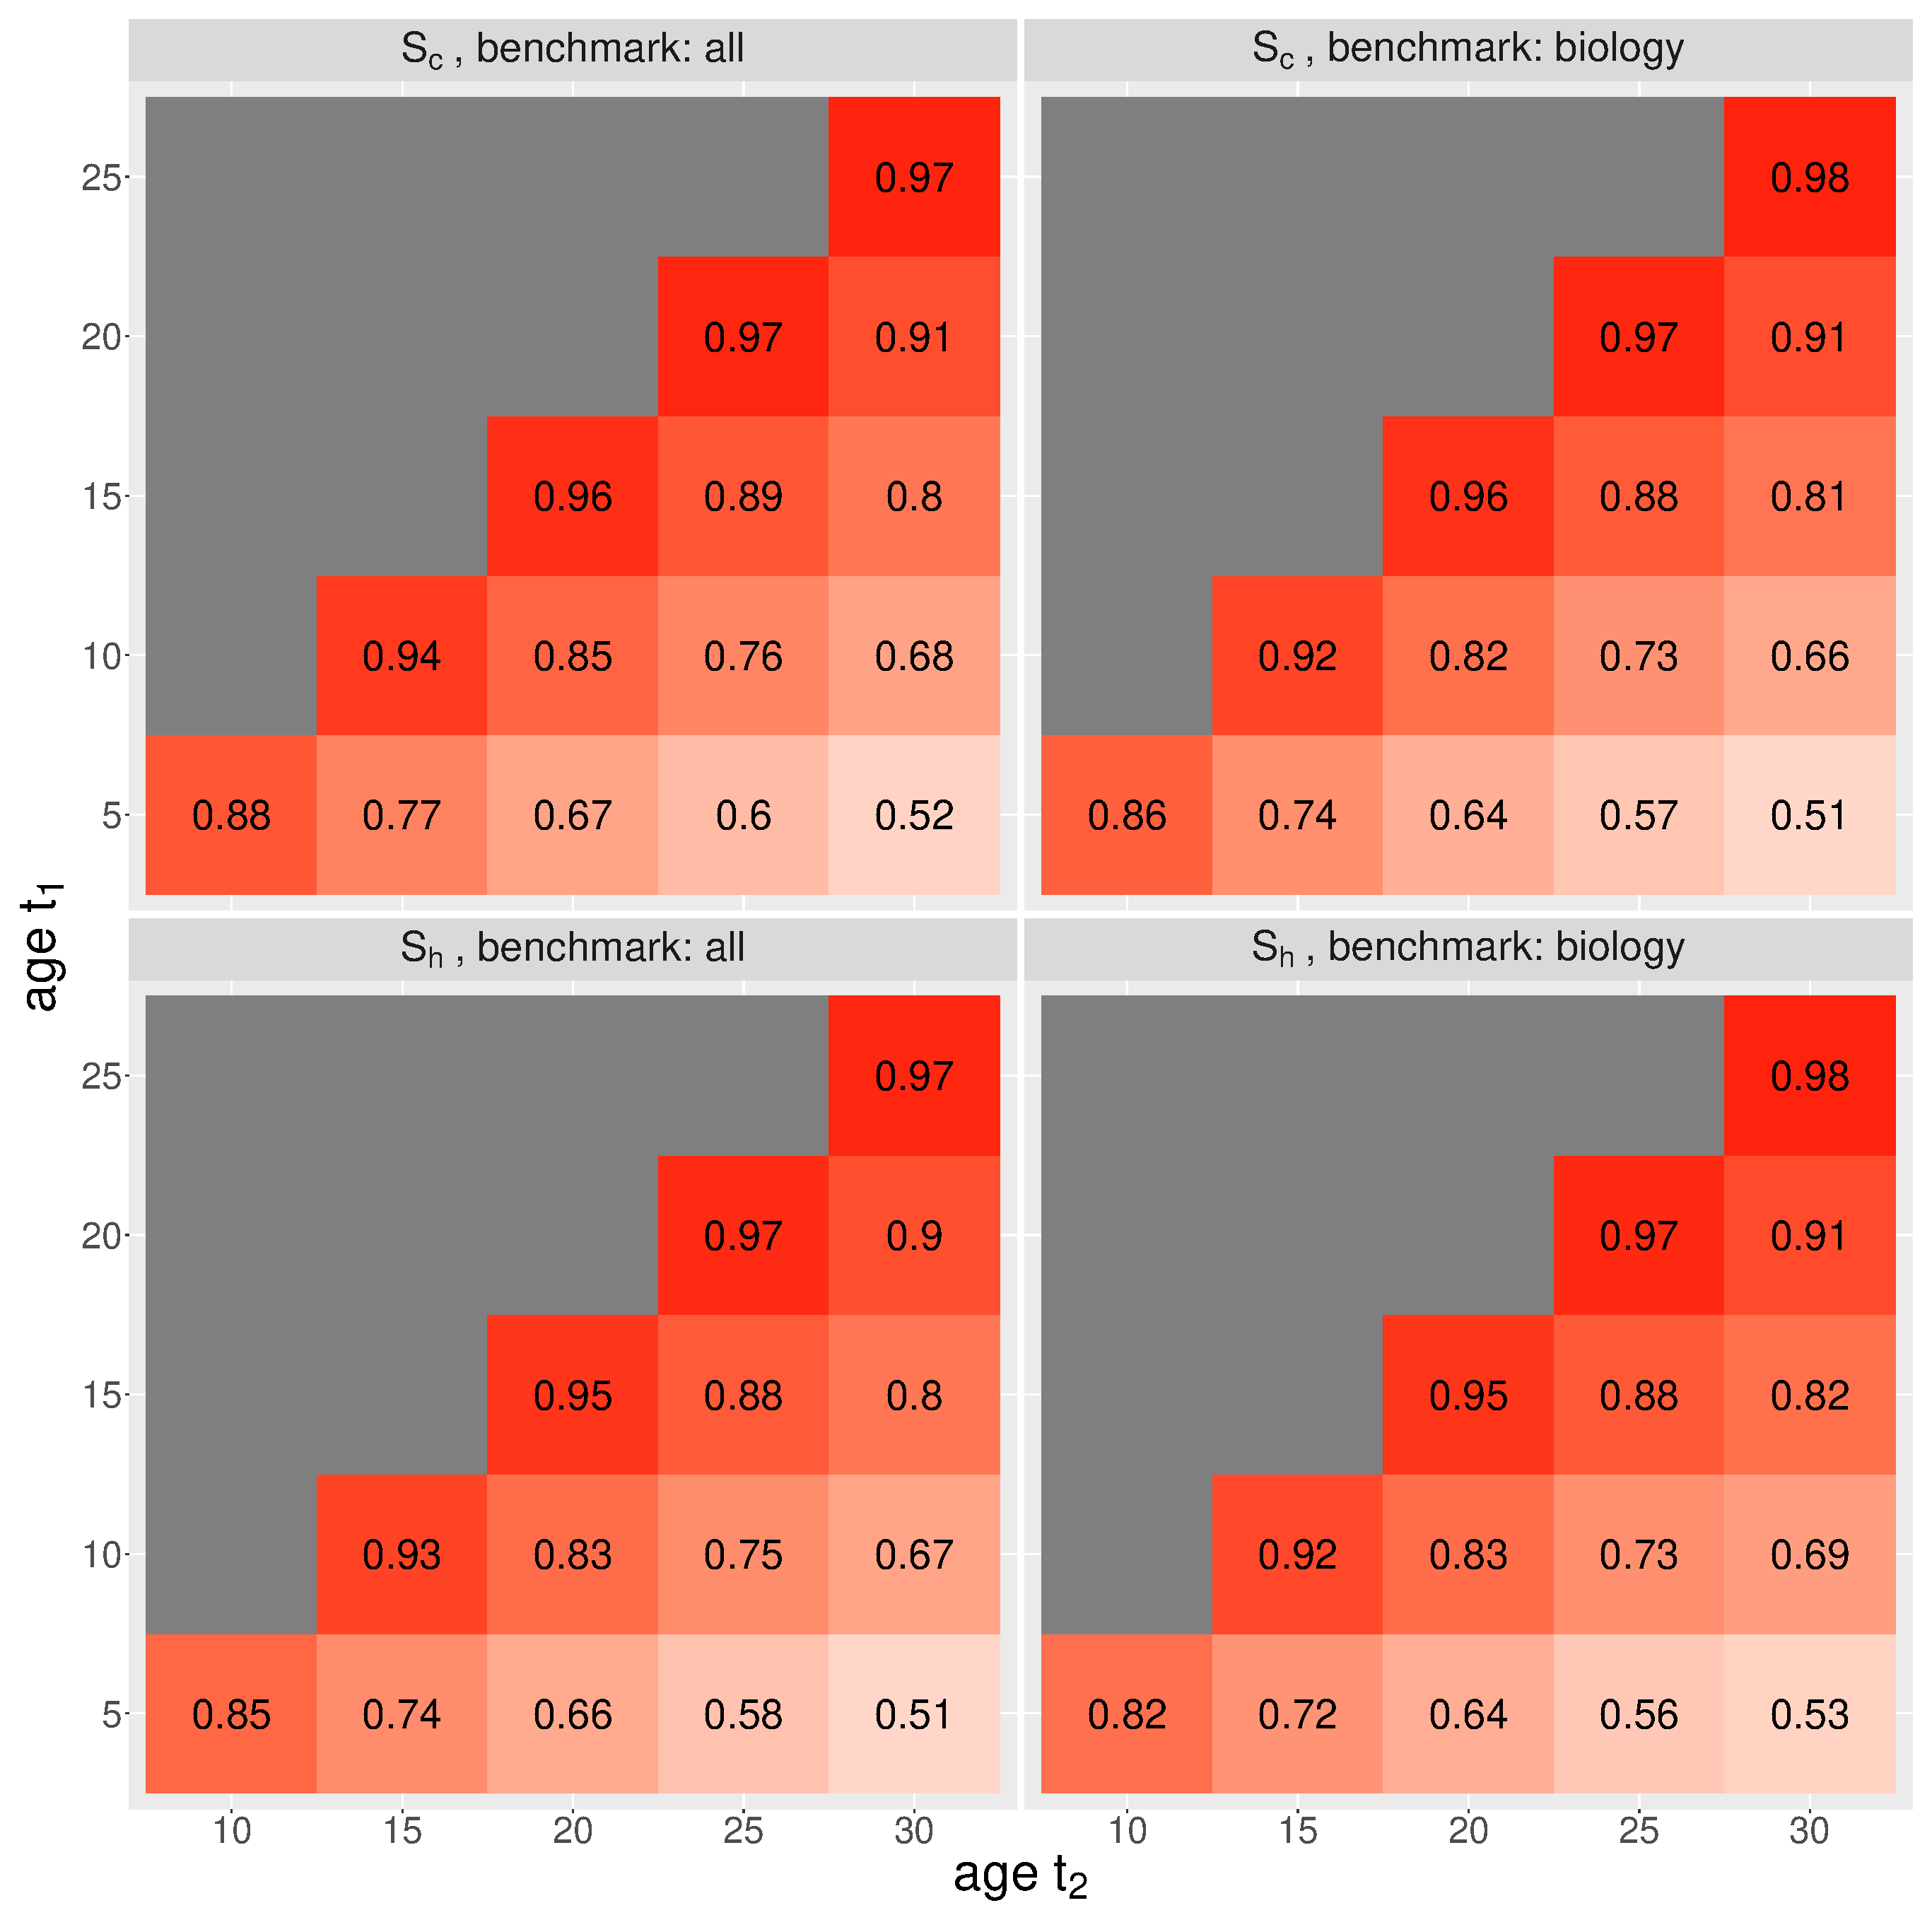
\includegraphics[width=\textwidth]{figures/pred_power/suppl_heatmap_cor_current.eps}
    \caption{{\bf Pearson Correlation between Rank Percentiles at Different Ages.} 
    This supplements the results in Figure \ref{fig:hm_rp_aut}.}
    \label{fig:hm_autrp_current}
\end{figure}



\section{Robustness of \texorpdfstring{S$_{P5}$}{Lg}}
\label{sec:suppl_robustness_P5}

Recall that S$_{P5}^{i}(t)$ is calculated based on an aggregation of the performances of publications that scholar $i$ publishes by age $t$. Denote $\text{m}_{P5}^{i}(t)$ as the evaluation metric of scholar $i$ at age $t$ based on $\text{P}_{c}^{j}(5)$, that is $\text{m}_{P5}^{i}(t)= \sum_{j=1}^{N(t)} \text{P}_{c}^{j}(5)$, where $N(t)$ is the total number of publications of scholar $i$ by age $t$. We illustrated in the paper that P$_c^j(t)$ exhibits high stability over $t$, and hence P$_{c}^{j}(5)$ can be applied to represent the performance of the publication. 

We further demonstrate the robustness of S$_{P5}$ by considering a longer citation history for each publication. Figure \ref{fig:robustness_test_cor} illustrates that m$_{P5}^{i}(t)$ is highly correlated with m$_{P10}^{i}(t)$ at age $t=1,\cdots,30$, where m$_{P10}^{i}(t)= \sum_{j=1}^{N(t)} \text{P}_{c}^{j}(10)$. We also consider utilizing the maximum, mean and median values of P$_{c}^{j}(t)$, for instance m$_{Pmax}^{i}(t)= \sum_{j=1}^{N(t)} \max_{t^\prime}\text{P}_{c}^{j}(t^\prime)$. We see from Figure \ref{fig:robustness_test_cor} that these metrics also exhibit high correlations with m$_{P5}$. Furthermore, we perform a Wilcoxon paired signed-rank test to compare the differences between S$_{P5}^{i}(t)$ and S$_{P10}^{i}(t)$ at each age $t=1,\cdots,30$, and the p-values are close to $1$; indicating that the differences are not statistically significant. Similar conclusions can be drawn for other indicators being considered.

\begin{figure}[ht!]
    \centering
    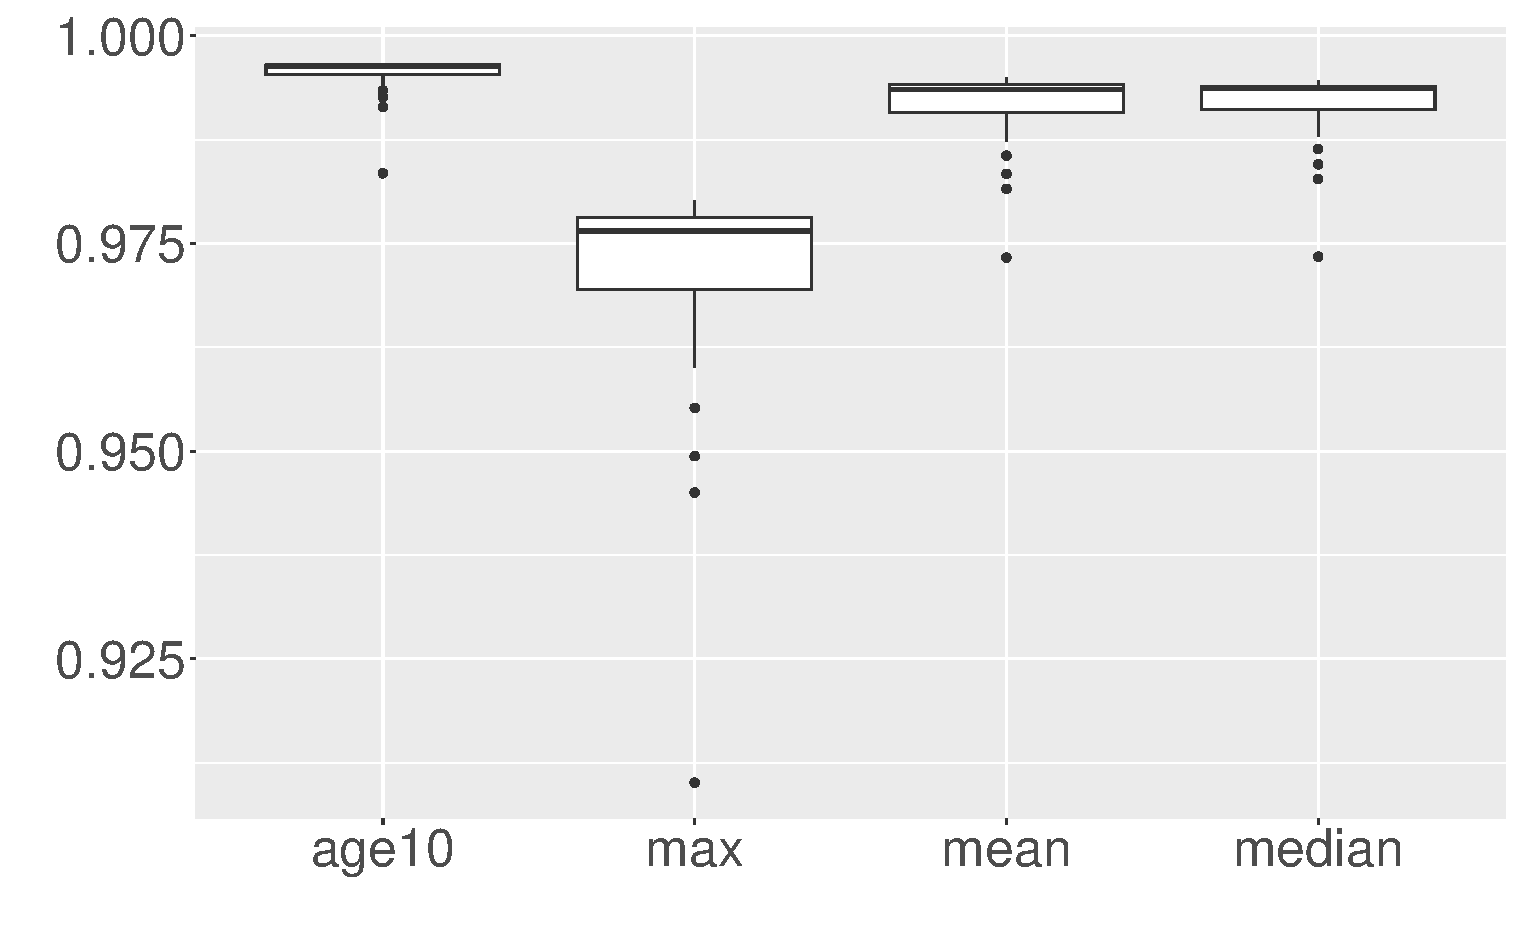
\includegraphics[width=0.7\textwidth]{figures/robustness/cor.eps}
    \caption{{\bf Correlation between m$_{P5}$ and Other Choices of Evaluation Metric.}
    The benchmark contains all scholars in the dataset. Age $10$, max, mean and median correspond to m$_{P10}$, m$_{Pmax}$, m$_{Pmean}$ and m$_{Pmedian}$, respectively. The correlation is calculated at each age $t=1,\cdots,30$.}
    \label{fig:robustness_test_cor}
\end{figure}


\iffalse
\begin{equation}
\label{eq:rp_matrix}
\bordermatrix{
    & \text{age 1}     & \text{age 2}     & \cdots & \text{age $K$}     \cr
    \text{paper 1}     & \text{rp}_{11}^{(c)}     & \text{rp}_{12}^{(c)}     & \ldots & \text{rp}_{1 K}^{(c)}      \cr
    \text{paper 2}     & \text{rp}_{21}^{(c)}     & \text{rp}_{22}^{(c)}    & \ldots & \text{rp}_{2 K}^{(c)}     \cr
    \quad \vdots & \vdots & \vdots & \ddots & \vdots \cr
    \text{paper $N$}     & \text{rp}_{N 1}^{(c)}     & \text{rp}_{N 2}^{(c)}     & \ldots  & \text{rp}_{N K}^{(c)}    \cr
}
\end{equation}

We take the maximum performance for each of the $N$ papers, and sum them:
\begin{equation}
    \omega_{i \tau} = \sum_{j=1,\cdots,N} \max_{k=1,\cdots, K} \text{rp}_{j k} ^{(c)}.
\end{equation}
\fi

\section{Stationarity test}
\label{sec:suppl_stationarity}

Two commonly used statistical tests for stationarity are the Dicky-Fuller test~\cite{dickey1979distribution} and KPSS test~\cite{kwiatkowski1992testing}. These two tests formulate the hypothesis testing problems differently. Dicky-Fuller test assumes a unit root presented in the series. A unit root means that the series is $I(1)$, i.e. integrated order $1$ and the first differenced series is stationary. The more negative the test statistic is, the stronger the rejection of the null. On the other hand, KPSS test assumes the null as the series being stationary, i.e. $I(0)$. KPSS test is slightly more general since it allows testing a series being non-stationary but does not present a unit root. The more positive the test statistic is, the stronger the rejection of the null. Both tests include the drift in the test equations but exclude the trend, since we do not observe significant trends in the series. 

The test statistics are shown in Figure \ref{fig:stationarity_test}. The dashed lines indicate the critical values at $5 \%$ level. KPSS test indicates that P$_c$ and S$_{P5}$ are non-stationary series, and we do not have enough evidence to reject them being $I(1)$ according to the Dicky-Fuller test. Furthermore, the differenced series are stationary based on both tests.


\begin{figure}[ht!]
    \centering
    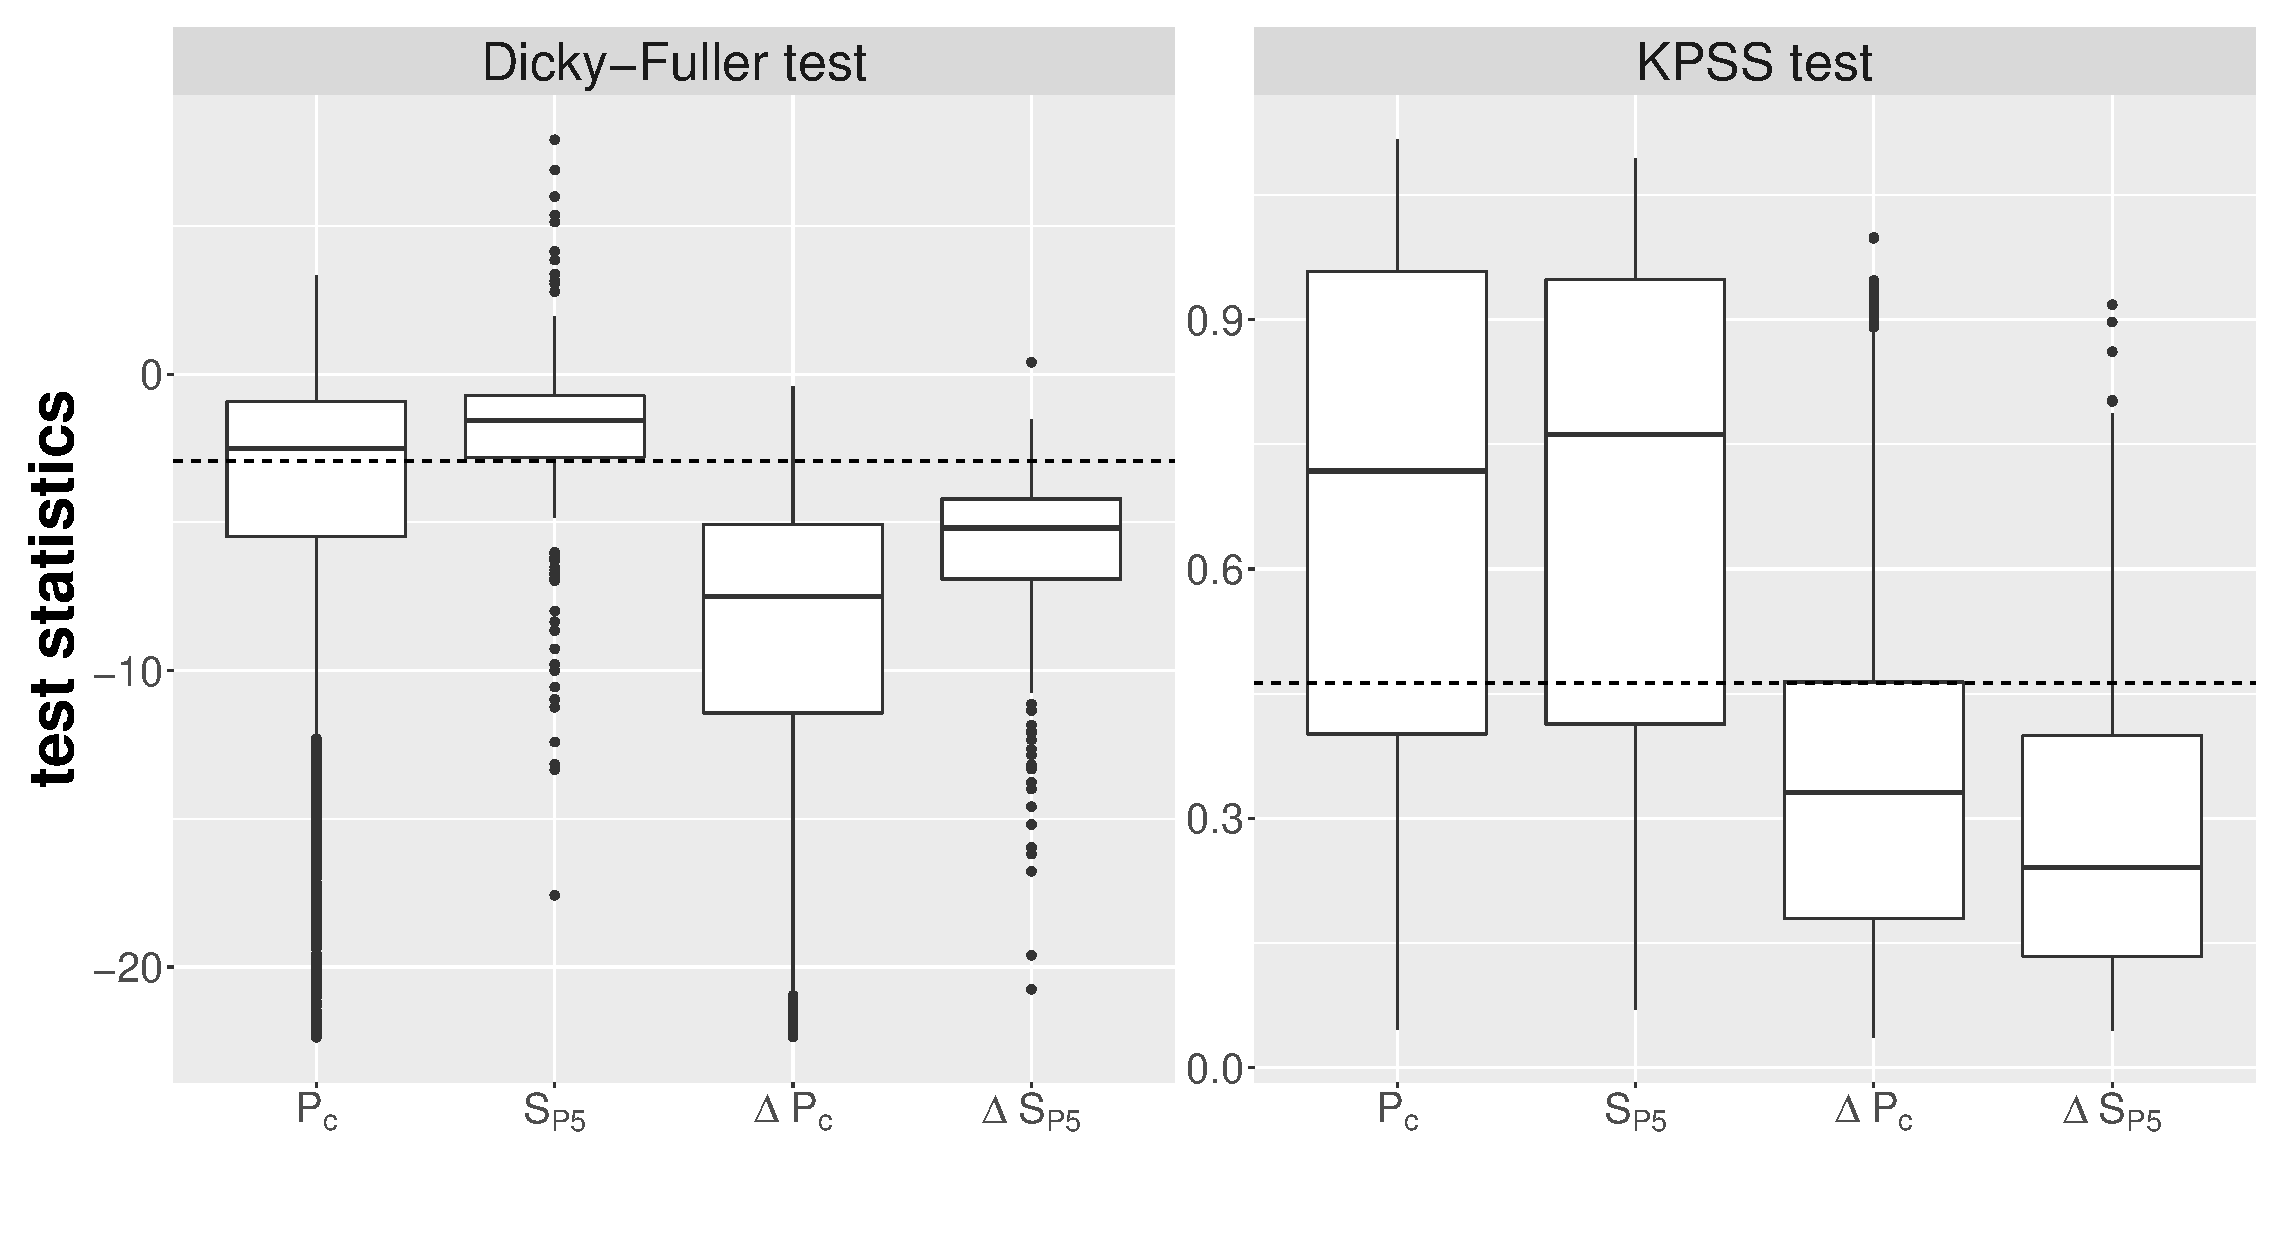
\includegraphics[width=\textwidth]{figures/stationarity/df_kpss.eps}
    \caption{{\bf Statistical Tests for the Stationarity of Rank Percentile Series.}
    Both tests are applied on every individual series, and the test statistics are presented. The $5\%$ critical value for each test is illustrated by the dashed horizontal line. Both tests suggest that publication indicator P$_c$ and scholar indicator S$_{P5}$ are non-stationary, while their differenced series are stationary. }
    \label{fig:stationarity_test}
\end{figure}

\iffalse
\section{Details of the predictive models}
\label{sec:suppl_details_predmodel}

The details of the predictive models are described below.
\begin{itemize}
    \item Baseline: simple linear regression of P$_{it_2}^c$ on P$_{it_1}^c$. Same applies for S$_{it}^{P5}$.
    \item Simple Markov model (sm): linear regression of P$_{it_2}^c$ on P$_{it_1}^c$ and the change of P$_{it}^c$ over the last $2$ ages, i.e. P$_{it_1}^c$-P$_{it_1-2}^c$. Same applies for S$_{it}^{P5}$.
    \item Penalized linear regression models, including the ridge, lasso, elastic net (enet) and the Gamma lasso (gamlr): linear models with different penalties on the regression coefficients. All of these methods shrink the coefficients towards zero, and the later three methods can provide sparse solutions (shrink the coefficients to be exactly zeros). 
    \item Ensemble methods of regression trees, including the random forest (rf) and extreme gradient boosting trees (xgbtree): rf is a bagging of regression trees with a subset of randomly selected features chosen at each split to avoid overfitting. xgbtree is a fast implementation of gradient boosting on regression trees with a model formation that emphasizes the role of regularizations to avoid overfitting.
    %\item Support vector regression (svr)~\cite{drucker1997support}: 
    \item Neural networks (nnet): feedforward networks with multiple hidden layers, and using dropout and $l_2$ regularization to avoid overfitting.
\end{itemize}
\fi


\begin{table}[htbp]
  \centering
    \begin{tabular}{l|l}
    Method & Tuning parameters \\
    \midrule
    Lasso & Penalty strength parameter \\
    \midrule
    Ridge & Penalty strength parameter \\
    \midrule
    \multirow{2}[2]{*}{Elastic net} & Penalty strength parameter \\
          & Penalty gap parameter \\
    \midrule
    \multirow{2}[2]{*}{Gamma lasso} & Penalty strength parameter \\
          & Convexity parameter \\
    \midrule
    \multirow{3}[2]{*}{Random forest} & Number of trees to grow \\
          & Number of variables used at each split \\
          & Minimum number of observations in a node \\
    \midrule
    \multirow{9}[2]{*}{xgbtree} & Maximum number of iterations \\
          & Learning rate \\
          & Regularization parameter \\
          & Maximum depth of the tree \\
          & Minimum number of observations in each child leaf \\
          & Number of observations supplied to a tree \\
          & Number of features supplied to a tree \\
          & Regularization parameter for ridge penalty \\
          & Regularization parameter for LASSO penalty \\
    \midrule
    \multirow{5}[1]{*}{Deep neural network} & Number of layers  \\
          & Learning rate \\
          & Number of hidden units at each layer \\
          & Dropout rate \\
          & Regularization parameter \\
    \end{tabular}%
  \caption{{\bf Hyperparameter(s) of the Machine Learning Models.}}
  \label{tab:hyperpara}%
\end{table}%

\begin{table}[htbp]
  \centering
    \begin{tabular}{l|l}
    Feature & Description \\
    \midrule
    pub\_cit\_cumulative & total citations of publication $j$ \\
    pub\_cit\_yearly & yearly citations of publication $j$ received in $t_1$ \\
    pub\_cit\_peryear & average citations of publication $j$ over age \\
    pub\_rp\_cumulative & rank percentile indicator calculated based on total citations, i.e. P$_c^{j}(t_1)$ \\
    pub\_rp\_yearly & rank percentile indicator calculated based on yearly citations at $t_1$\\
          &  \\
    aut\_cit\_cumulative          & total citations of author $i$ \\
    aut\_cit\_yearly          & yearly citations of author $i$ at $t_1$ \\
    aut\_npub\_cumulative & total number of publications of author $i$ \\
    aut\_npub\_yearly & yearly number of publications of author $i$ at $t_1$ \\
    aut\_cit\_perpaper & average citations per paper for author $i$  \\
    aut\_h\_index & h-index of author $i$  \\
    aut\_g\_index & g-index of author $i$ \\
    aut\_maxcit\_pub & largest citation that a single paper of author $i$ has received \\
    aut\_rprp5\_cumulative & rank percentile calculated based on all papers, i.e. S$_{P5}^{i}(t_1)$ \\
    aut\_rprp5\_yearly & rank percentile calculated based on just papers written at $t_1$ \\
          &  \\
    *\_delta & the difference over the last two ages for each of the above features \\
    \end{tabular}%
  \caption{{\bf Features for Predicting the Publication Impact.}}
  \label{tab:features_pubrp}%
\end{table}%

\begin{table}[htbp]
  \centering
    \begin{tabular}{l|l}
    Feature & Description \\
    \midrule
    aut\_cit\_cumulative & total citations of author $i$ \\
    aut\_cit\_yearly & yearly citations of author $i$ at age $t_1$ \\
    aut\_npub\_cumulative & number of publications of author $i$ \\
    aut\_npub\_yearly & yearly number of publications of author $i$ at age $t_1$ \\
    aut\_h\_index & h-index of author $i$ \\
    aut\_g\_index & g-index of author $i$ \\
    aut\_cit\_peryear & average citations per age of author $i$ \\
    aut\_rprp5\_cumulative & rank percentile calculated using all publications, i.e. S$_{P5}^{i}(t_1)$ \\
    aut\_rprp5\_yearly & rank percentile calculated using just publications written in age $t_1$ \\
          &  \\
    pub\_cit\_cumulative\_\{min,mean,max\} & citations received by each of the publications \\
    pub\_cit\_yearly\_\{min,mean,max\} & citations received by each of the publications written at age $t_1$ \\
    pub\_rp\_cumulative\_\{min,mean,max\} & publication rank percentiles calculated based on total citations \\
    pub\_rp\_yearly\_\{min,mean,max\} & publication rank percentiles calculated based on citations at age $t_1$ \\
          &  \\
    *\_delta & the difference over the last two ages for each of the above features \\
    \end{tabular}%
  \caption{{\bf Features for Predicting the Scholar Impact.}}
  \label{tab:features_autrp}%
\end{table}%





\clearpage
\section{Other tables and figures}
% exploratory statistics of the data
\begin{table}[ht]
\centering
\begin{tabular}{c|c|c|c}
 benchmark     & all   & biology & tenured \\
\midrule
\# publications & 801239 & 194713 & 176404 \\
\# scholars & 14358 & 3410  & 2706 \\
\# citations per publication by age 5  & 45    & 56    & 49 \\
\# citations per scholar by age 5 & 172   & 209   & 332 \\
\end{tabular}%
\caption{{\bf Summary statistics of the dataset. }}
\label{tab:exploratory}
\end{table}

% exploratory plots of the data
\begin{figure}[ht!]
    \centering
    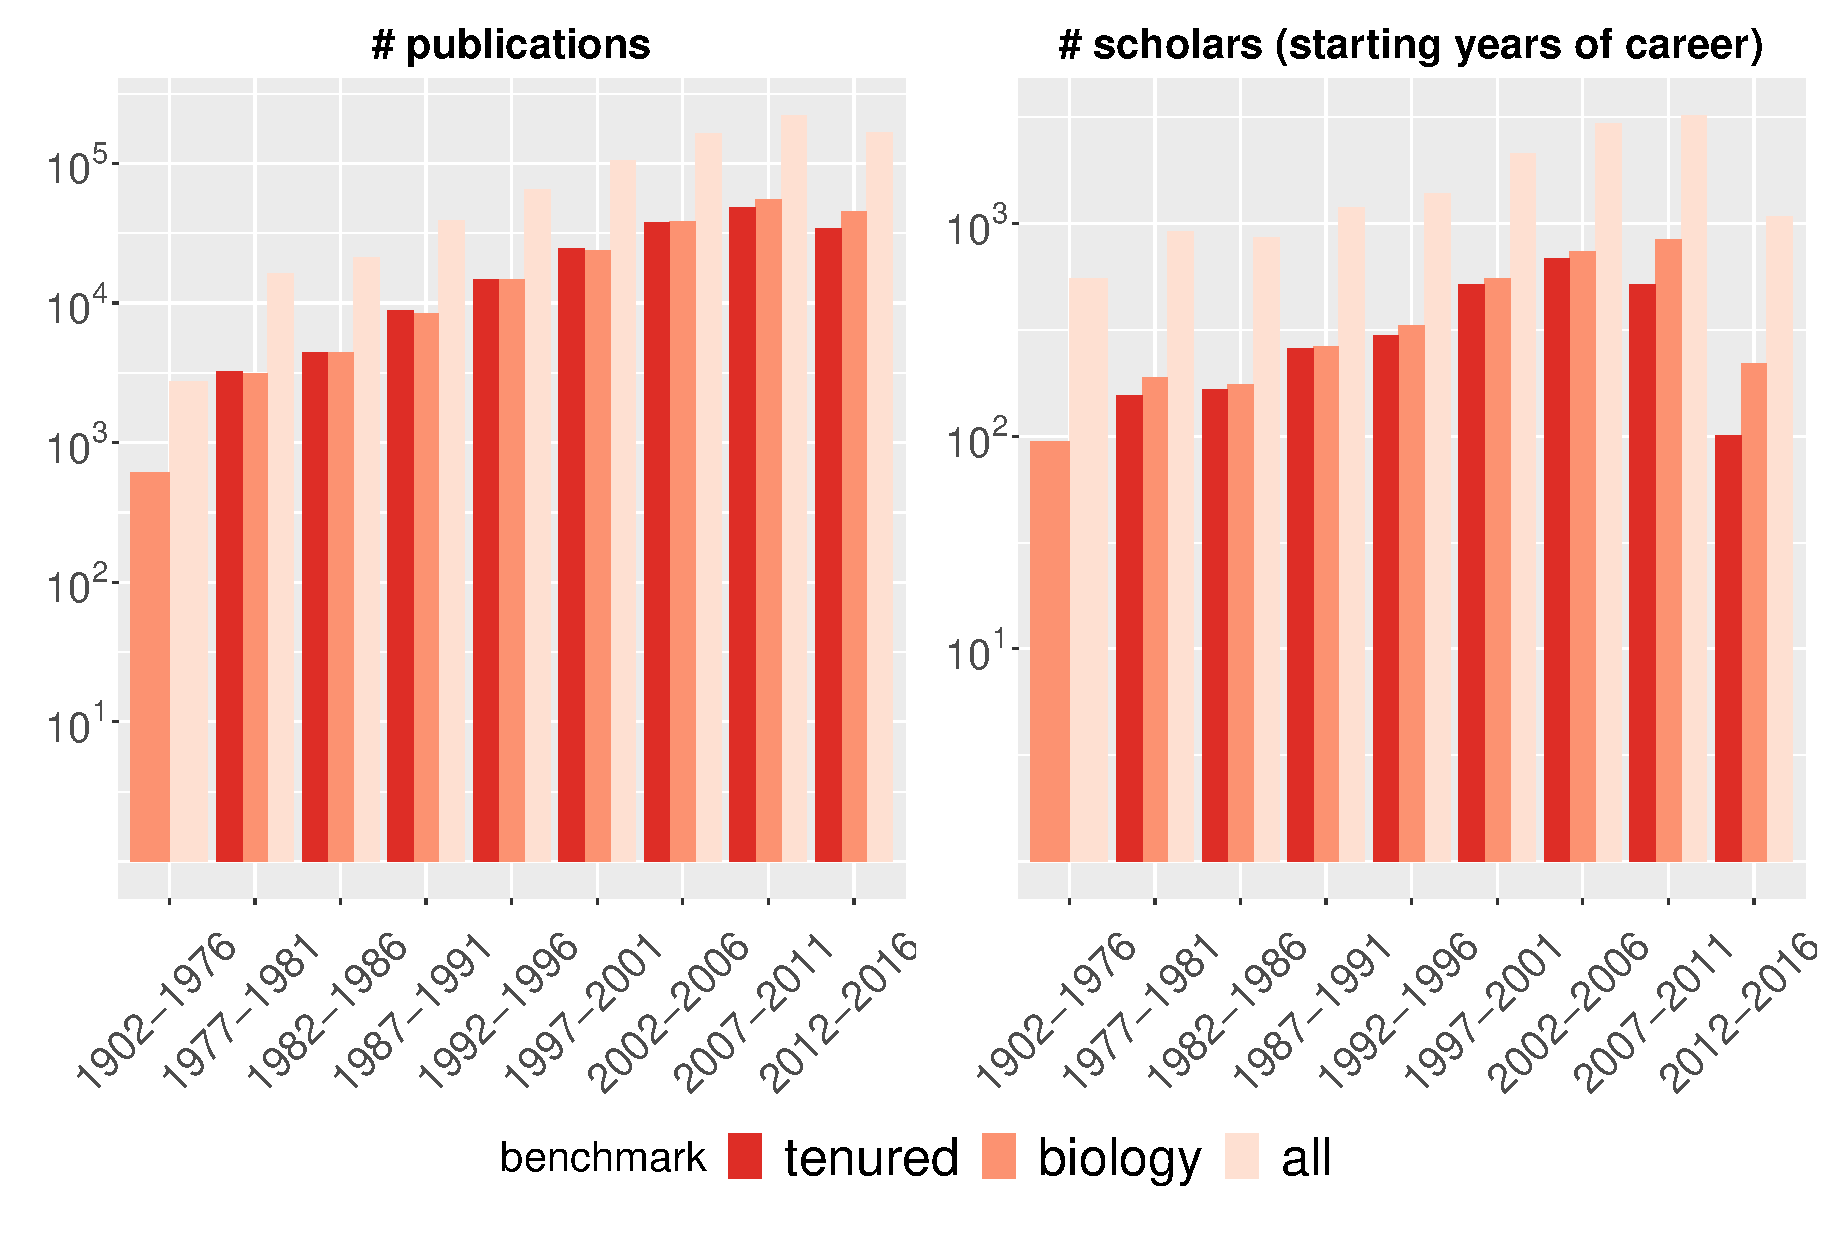
\includegraphics[width=0.8\textwidth]{figures/exploratory/npub_naut.eps}
    \caption{{\bf Exploratory Statistics of the Dataset.}
    \textbf{Left panel}: number of papers published in a certain period; \textbf{right panel}: number of authors who start their careers in a certain period. }
    \label{fig:exploratory}
\end{figure}

\begin{figure}[ht!]
    \centering
    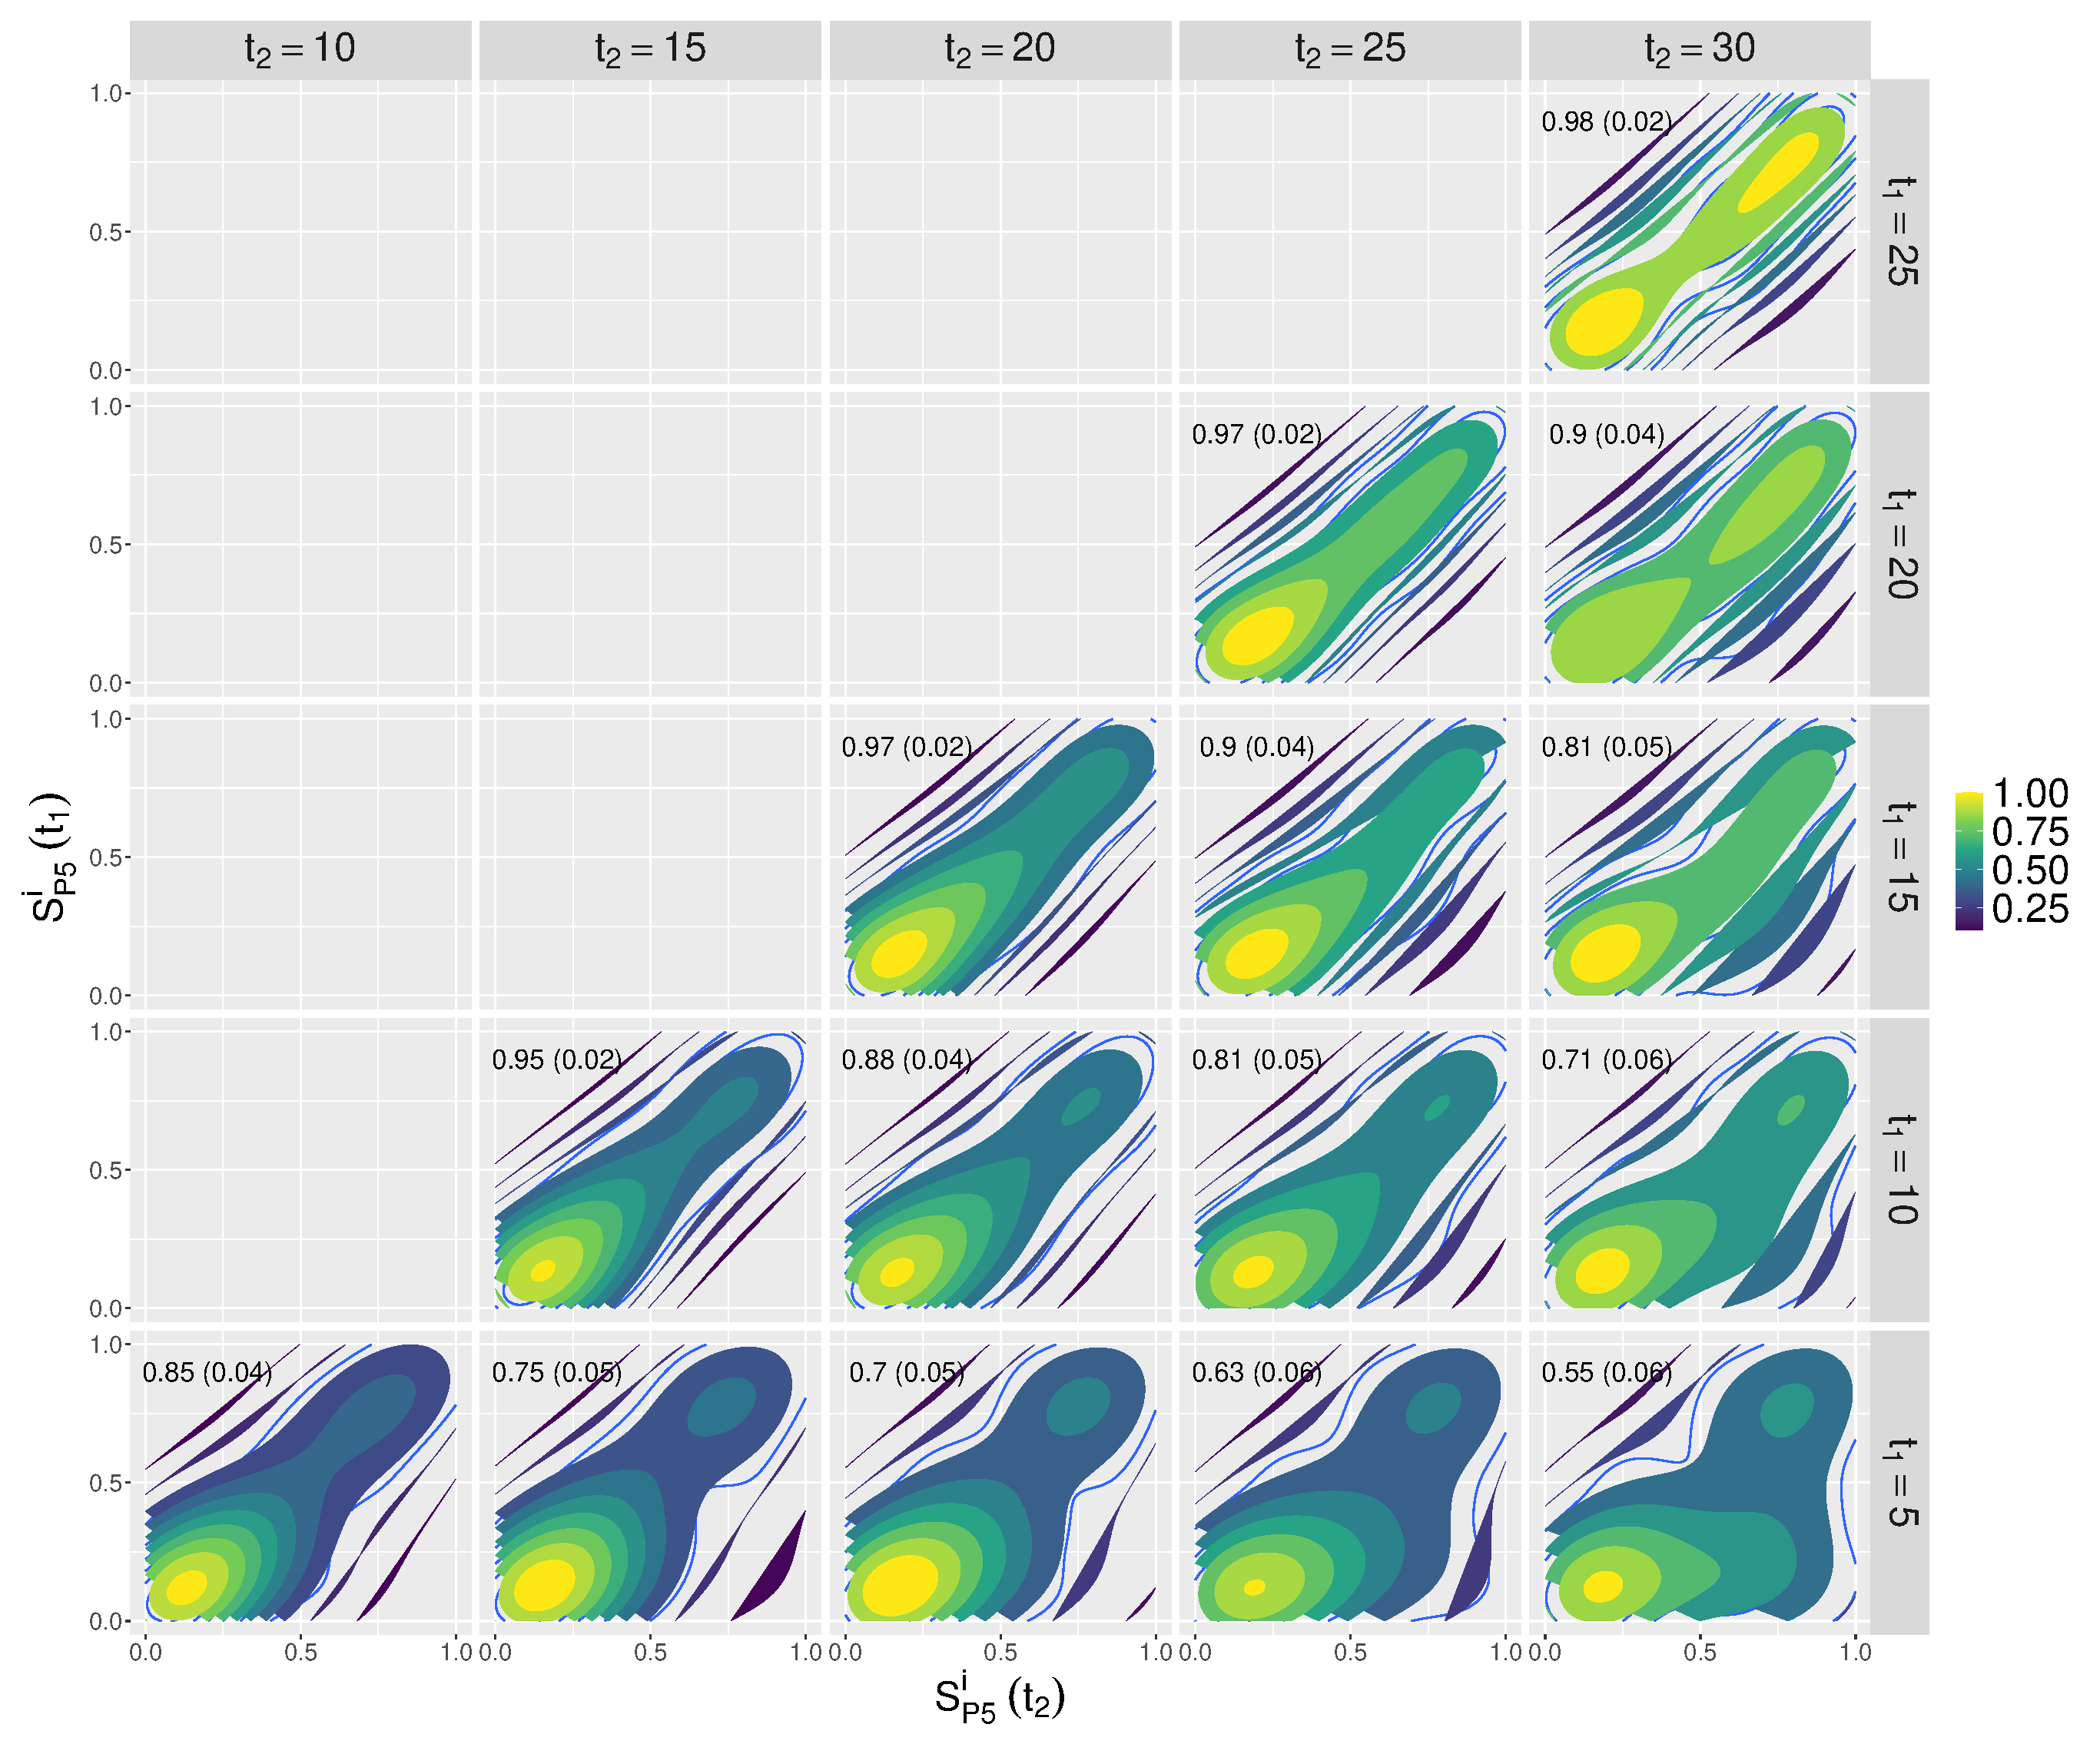
\includegraphics[width=\textwidth]{figures/pred_power/scatter_autrp_all.eps}
    \caption{{\bf Kernel Density Estimation for the Scatter Points of S$_{P5}^{i}(t_1)$ and S$_{P5}^{i}(t_2)$.}
    We fit a simple linear regression of S$_{P5}^{i}(t_2)$ on S$_{P5}^{i}(t_1)$. The estimated coefficient and the corresponding standard error (in the parentheses) are displayed in each plot. The benchmark contains all scholars in the dataset.}
    \label{fig:scatter_autrp_all}
\end{figure}


\begin{figure}[ht!]
    \centering
    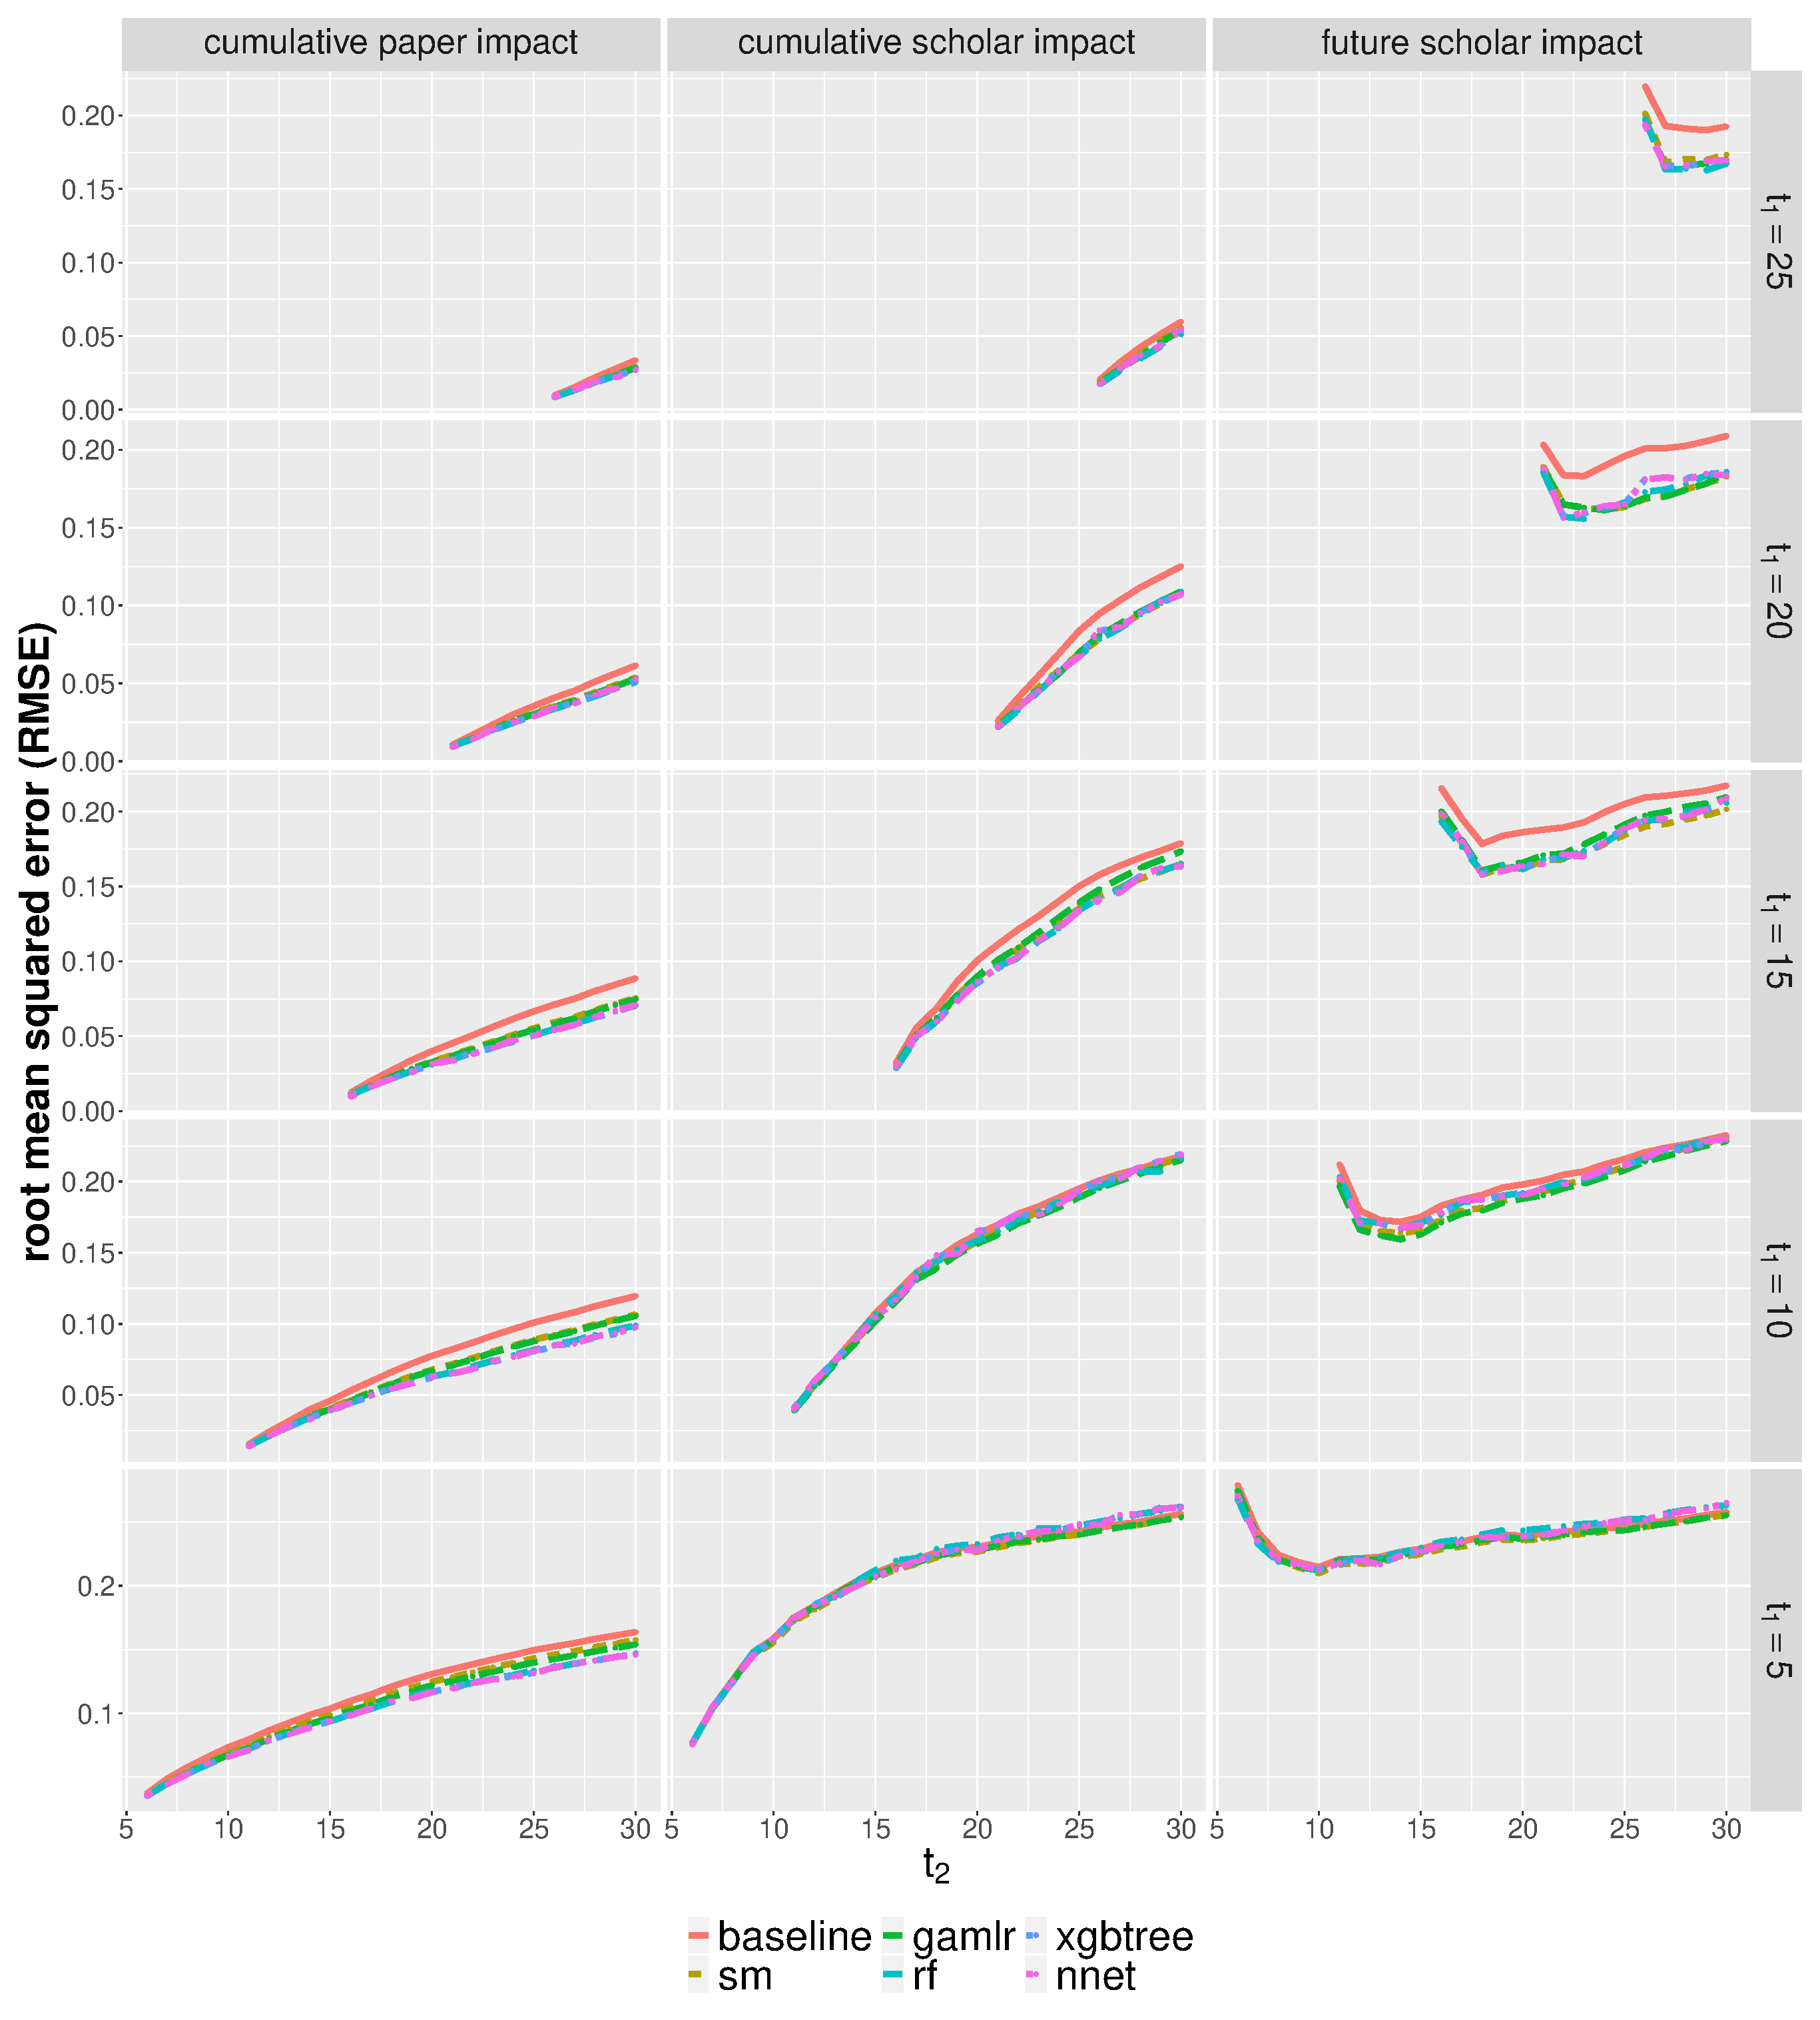
\includegraphics[width=\textwidth]{figures/pred_model/rmse.eps}
    \caption{{\bf RMSE for the Predictive Models.}}
    \label{fig:pred_rmse}
\end{figure}

\begin{figure}[ht!]
    \centering
    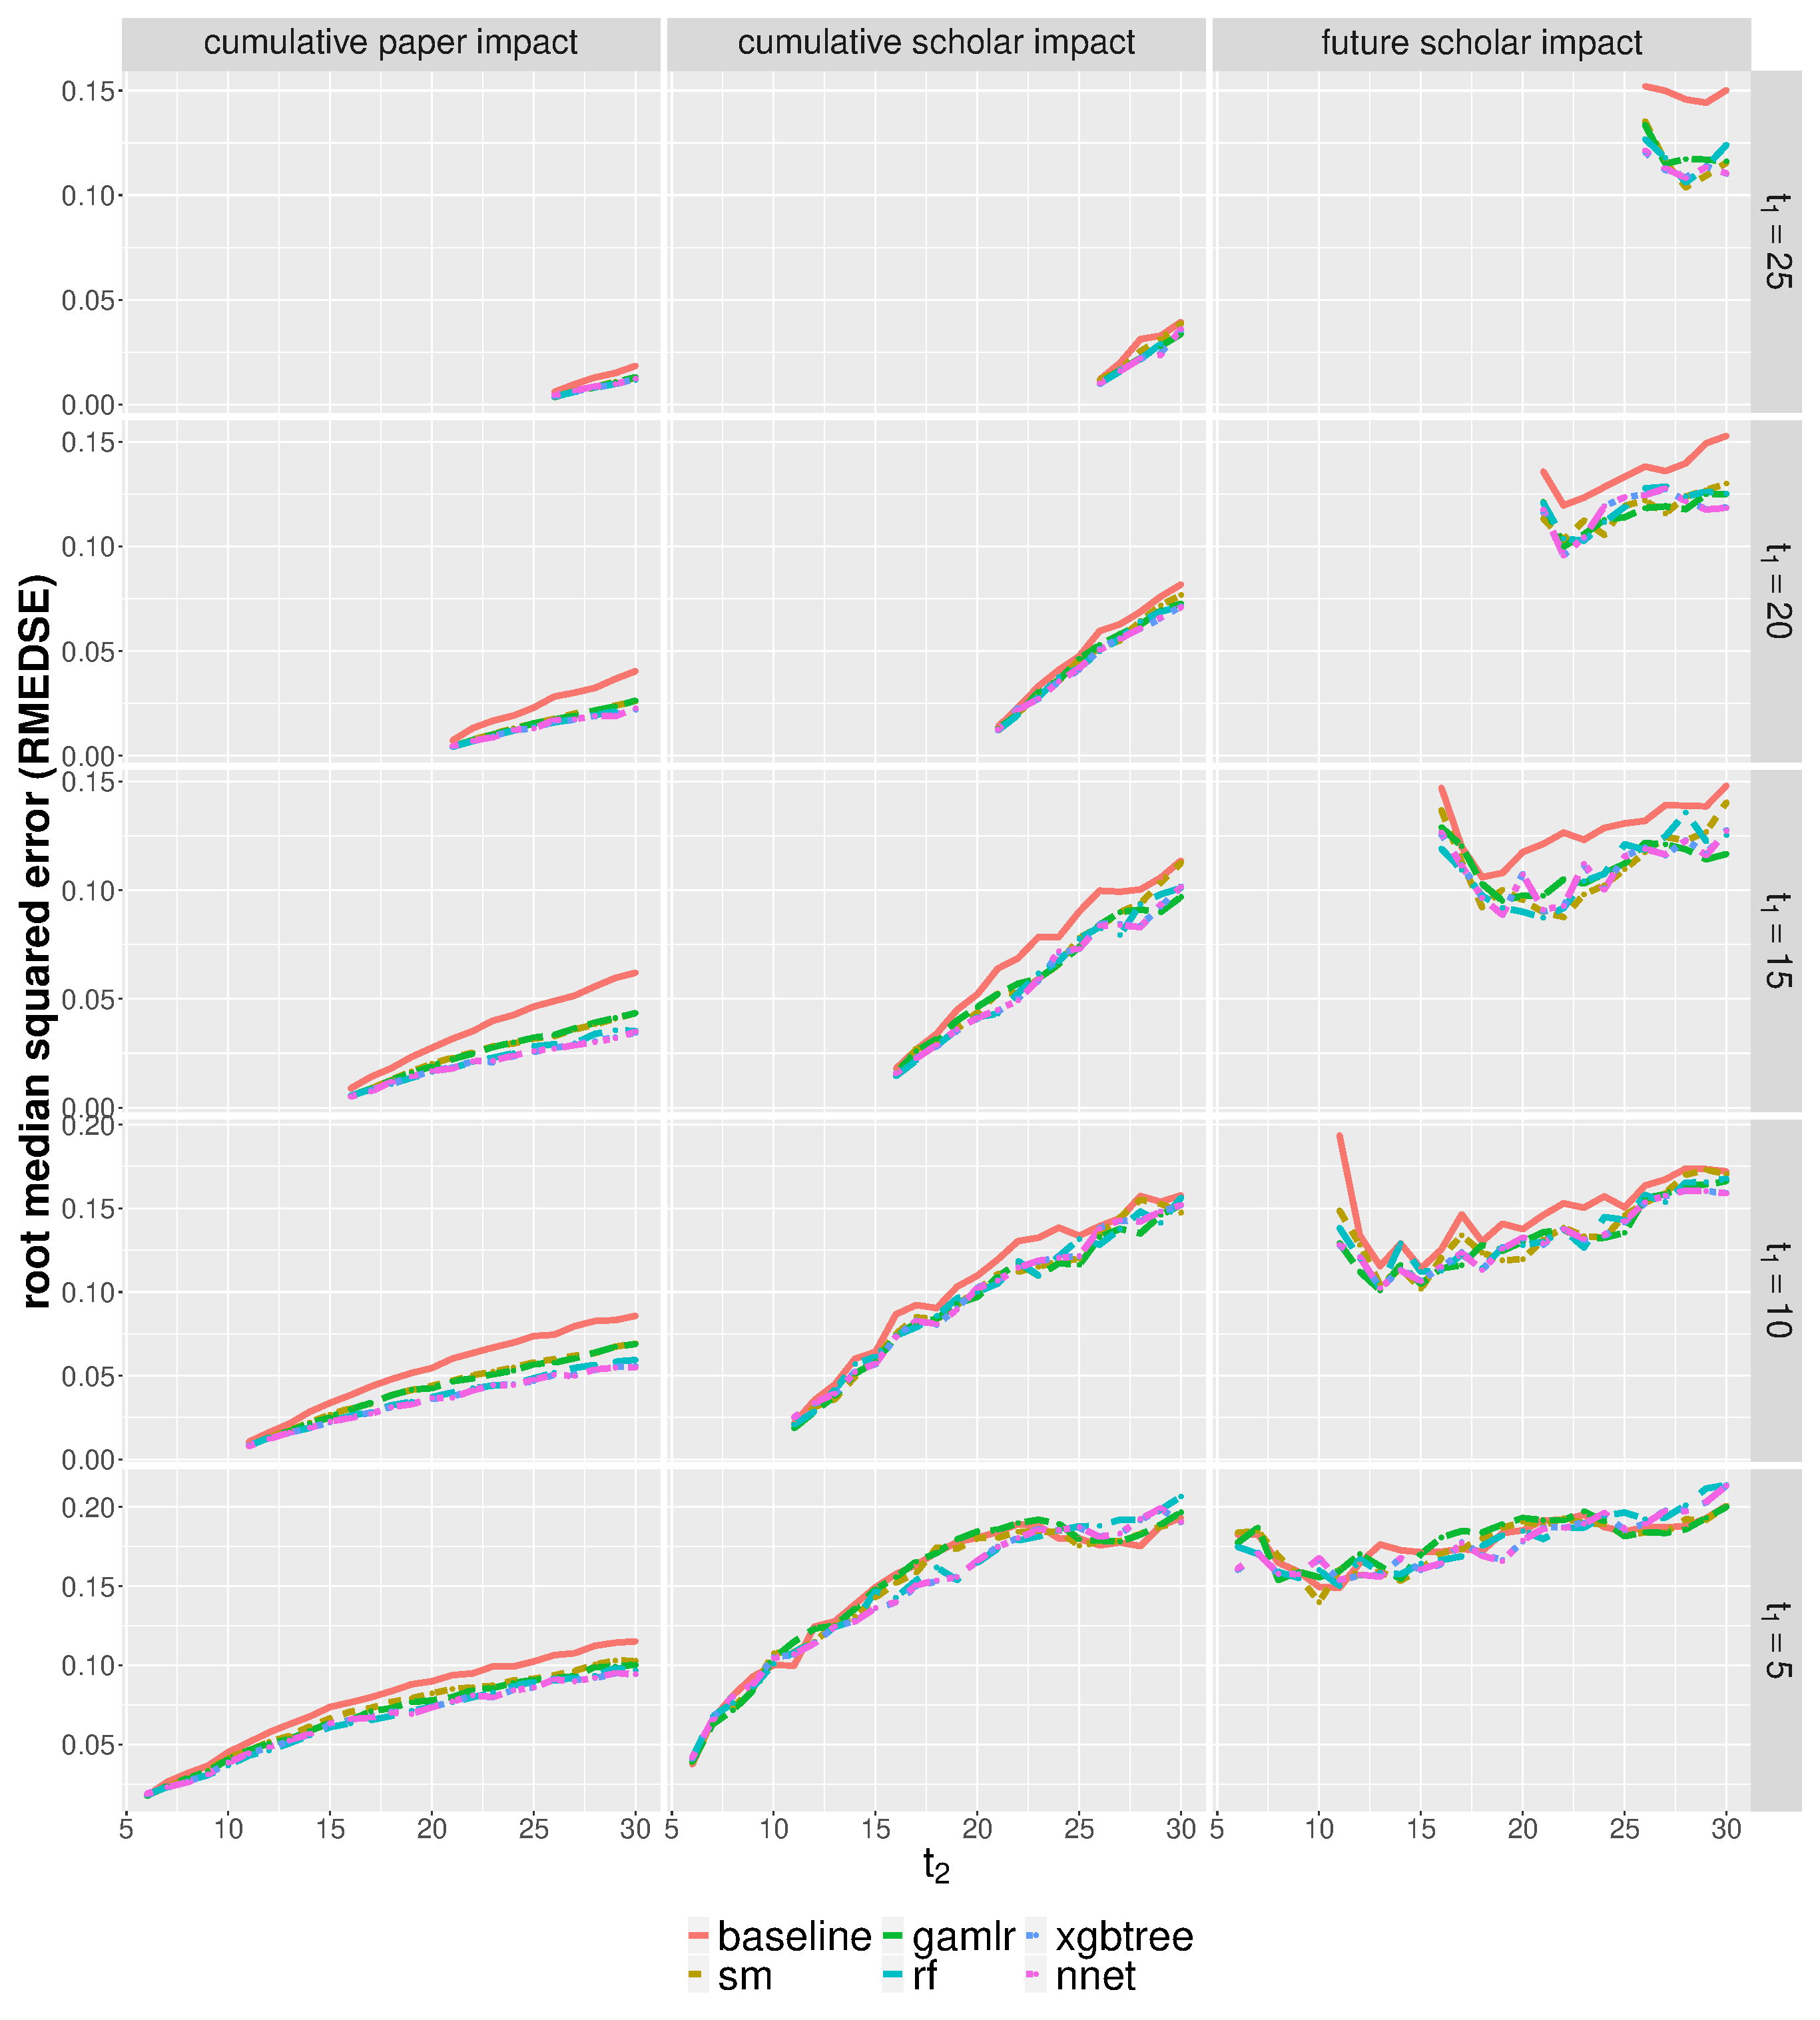
\includegraphics[width=\textwidth]{figures/pred_model/medse.eps}
    \caption{{\bf RMESE for the Predictive Models.}}
    \label{fig:pred_medse}
\end{figure}

\begin{figure}[ht!]
    \centering
    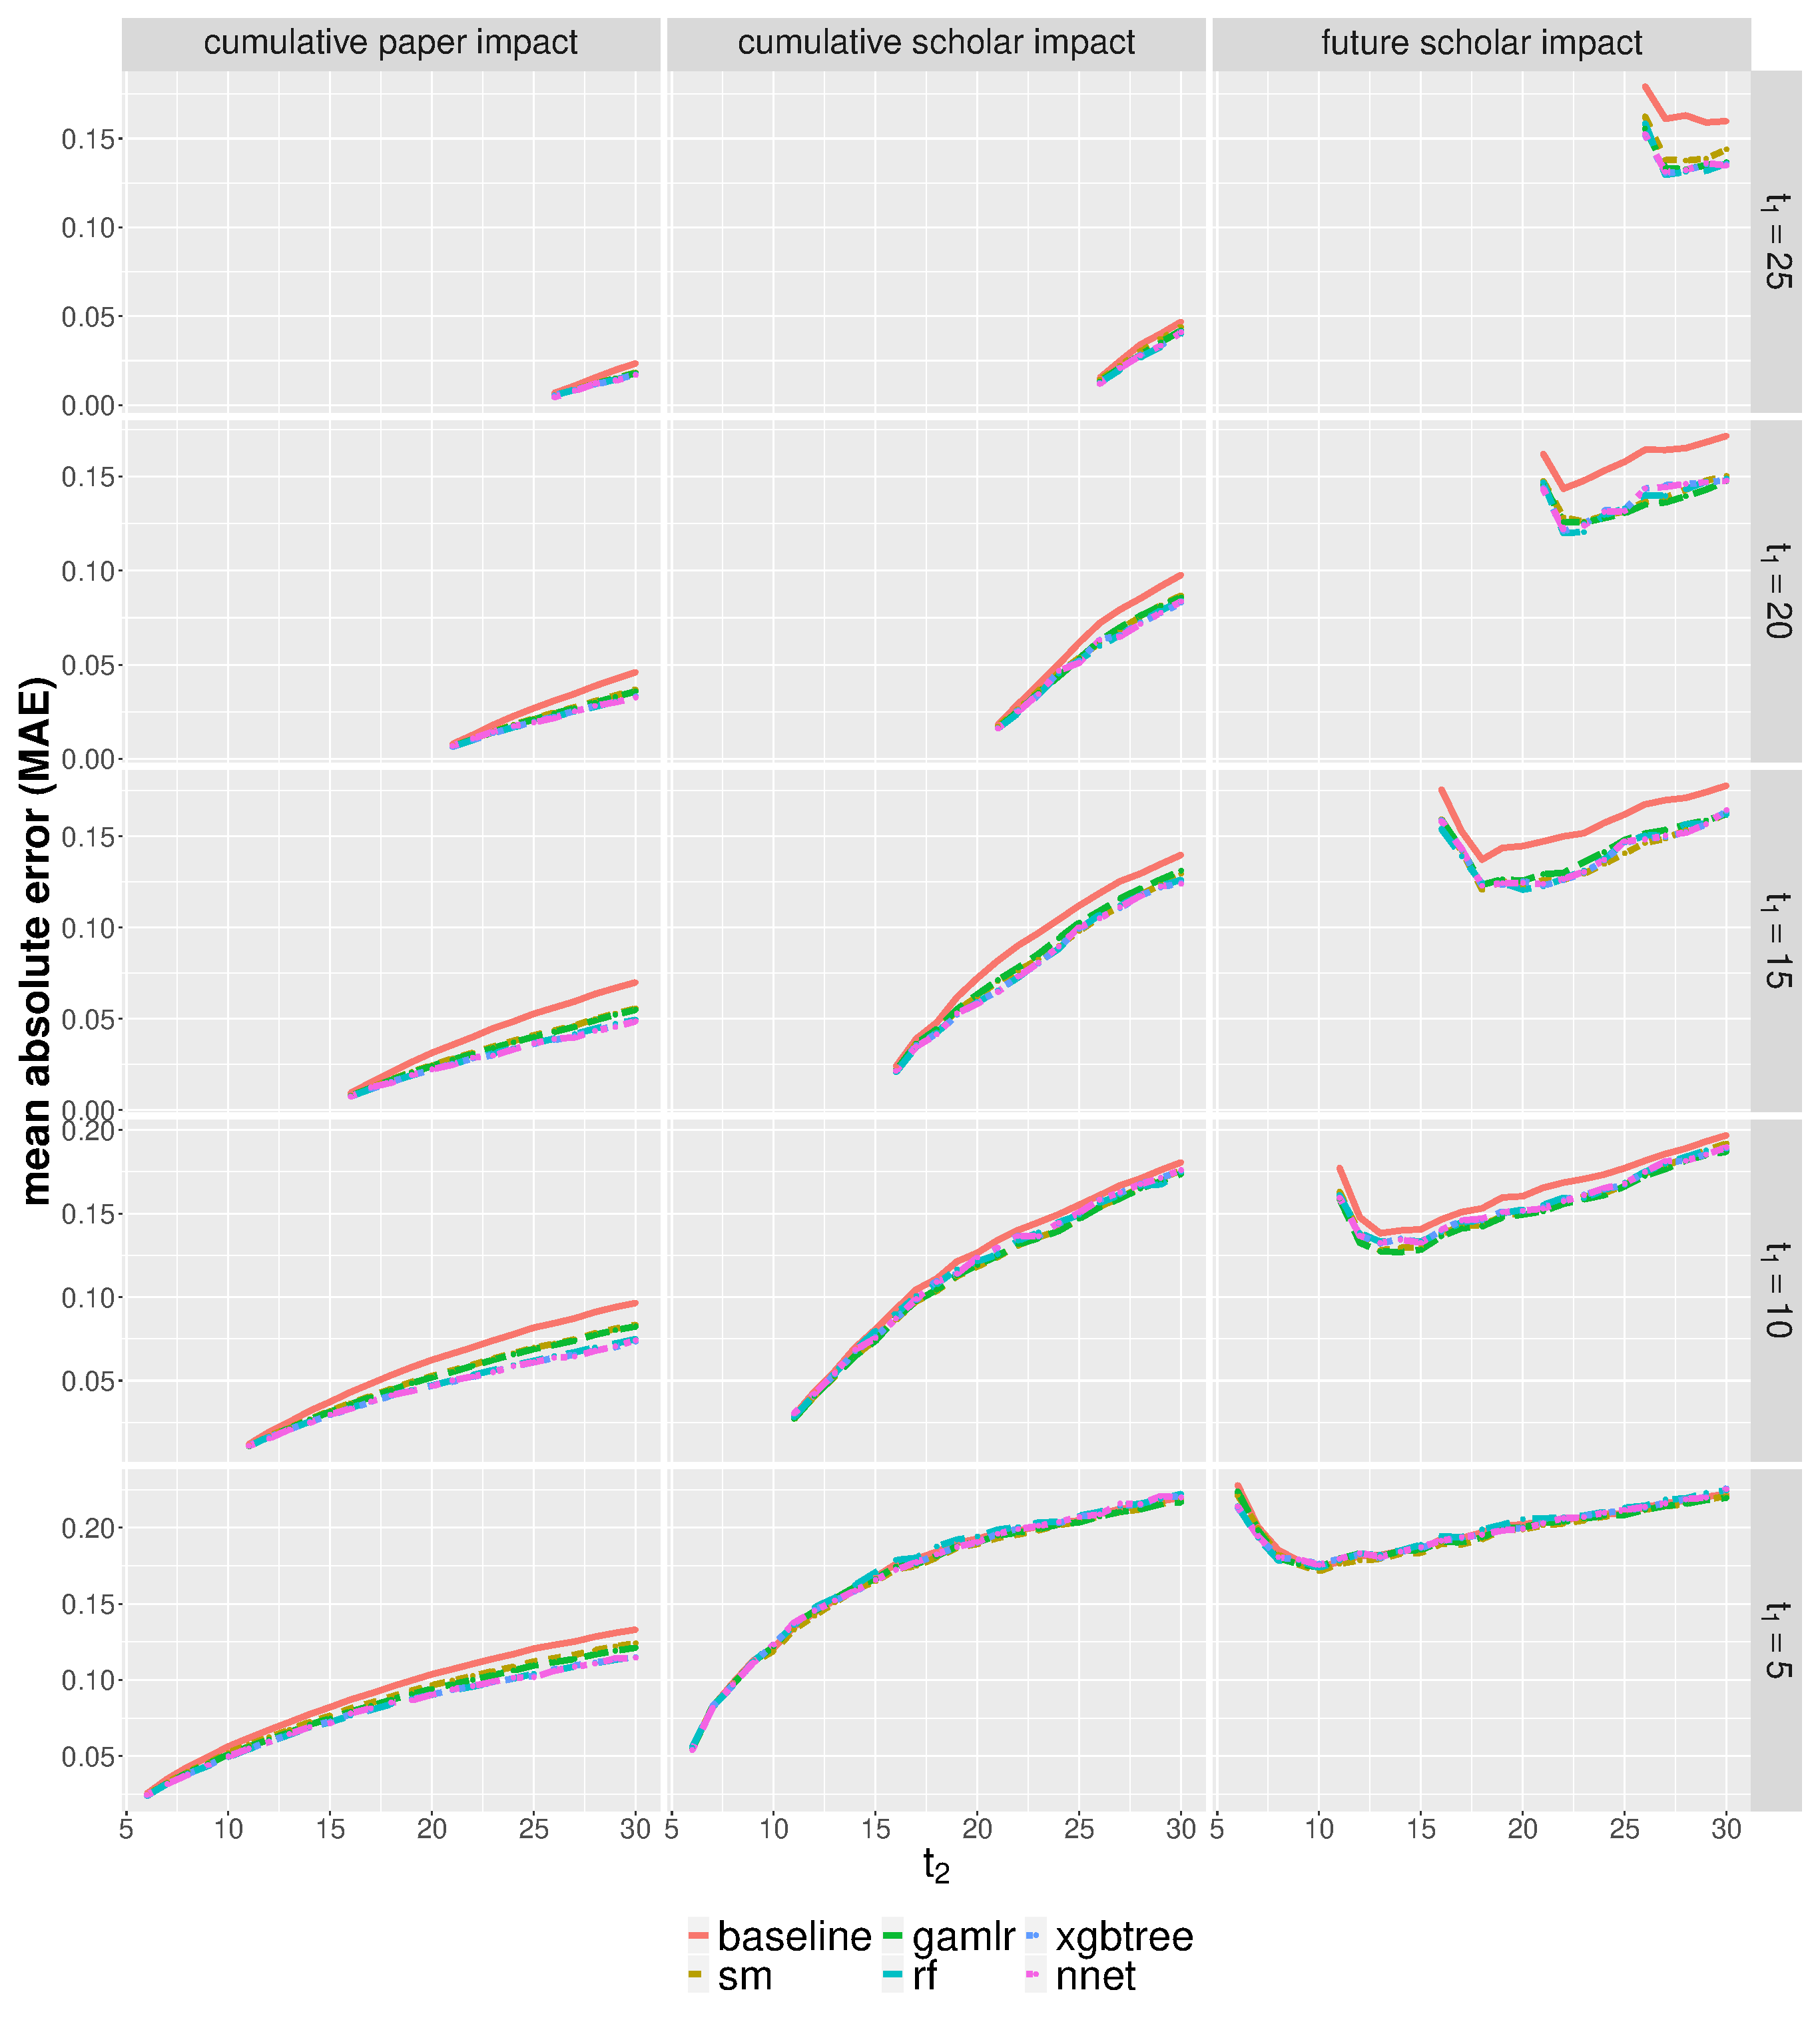
\includegraphics[width=\textwidth]{figures/pred_model/mae.eps}
    \caption{{\bf MAE for the Predictive Models.}}
    \label{fig:pred_mae}
\end{figure}

\iffalse
\clearpage
Three effects may lead to the non-stationarity of rank percentile for scholars are:
\begin{itemize}
  \item Seniority effect of scholars: senior scholars can attract more citations than junior scholars. In figure \ref{fig:seniority}, we see that senior authors (e.g. those starting their careers in 1980s) do not have an advantage over junior authors (e.g. those starting their careers in 2000s). 
  \item Time effect: papers published more recently attract more citations than papers published $20$ years ago. This maybe due to the fact that the entire scientific community is growing, and we have much more scholars now than $20$ years ago, which makes the paper visible to a larger audience and potentially attracts more citations. Meanwhile, as Internet and especially social media becomes vital, papers now have much better visibility than those $20$ years ago. Figure \ref{fig:environment} shows that for the scholars starting their careers in $1980$, more recent papers attract more citations than old papers. Since we've already filtered out the seniority effect of the scholars, this is result from external effects. 
  \item Number of publications: scholars now tend to produce more publications than scholars say $20$ years ago. Evidence is shown in figure \ref{fig:npub}. 
\end{itemize}
We now fix the bias from the time effect and number of publications, in order to get stationary rank percentile indicators for scholars. Let's say we have a scholar $i$ who starts his/her career in physical year $Y_i$. For a paper $j$ that the scholar publishes in physical year $Y_j$, we calculate its rank percentile rp.c$_{j5}$ where the benchmark contains all the papers that are published in year $Y_j$. By restricting the benchmark in such way, we potentially remove the time effect. We repeat the process for all the papers of scholar $i$ that are published by age $t$ and obtain the metric $\sum_{j=1}^{N_t^{(i)}} \text{rp.c}_{j5}$. Furthermore, we calculate a rank percentile indicator rp.p$_{it}$ based on the number of publications by age $t$, and the benchmark is all the scholars who start their careers in physical year $Y_i$. Finally, we have the evaluation metric m$_{it} = \text{rp.p}_{it} \cdot \sum_{j=1}^{N_t^{(i)}} \text{rp.c}_{j5}$. The rank percentile indicator, denoted as rp.rp5, can be then computed based on m$_{it}$ and the benchmark is all or biology. 

Figure \ref{fig:compare_autrp} shows various types of scholar rank percentile indicators. Both rp.c and rp.h, that are based on total citations and h-index, show advantages for junior scholars due to the reasons explained above. However, rp.rp5 seems to be stationary. 


\begin{figure}[h!]
     \centering
     \begin{subfigure}[b]{0.48\textwidth}
         \centering
         
\includegraphics[width=\textwidth]{figures/exploratory/seniority_age5.eps}
         \caption{Total citations by age $5$ for papers published in $2012$}
     \end{subfigure}
     \hfill
     \begin{subfigure}[b]{0.5\textwidth}
         \centering
         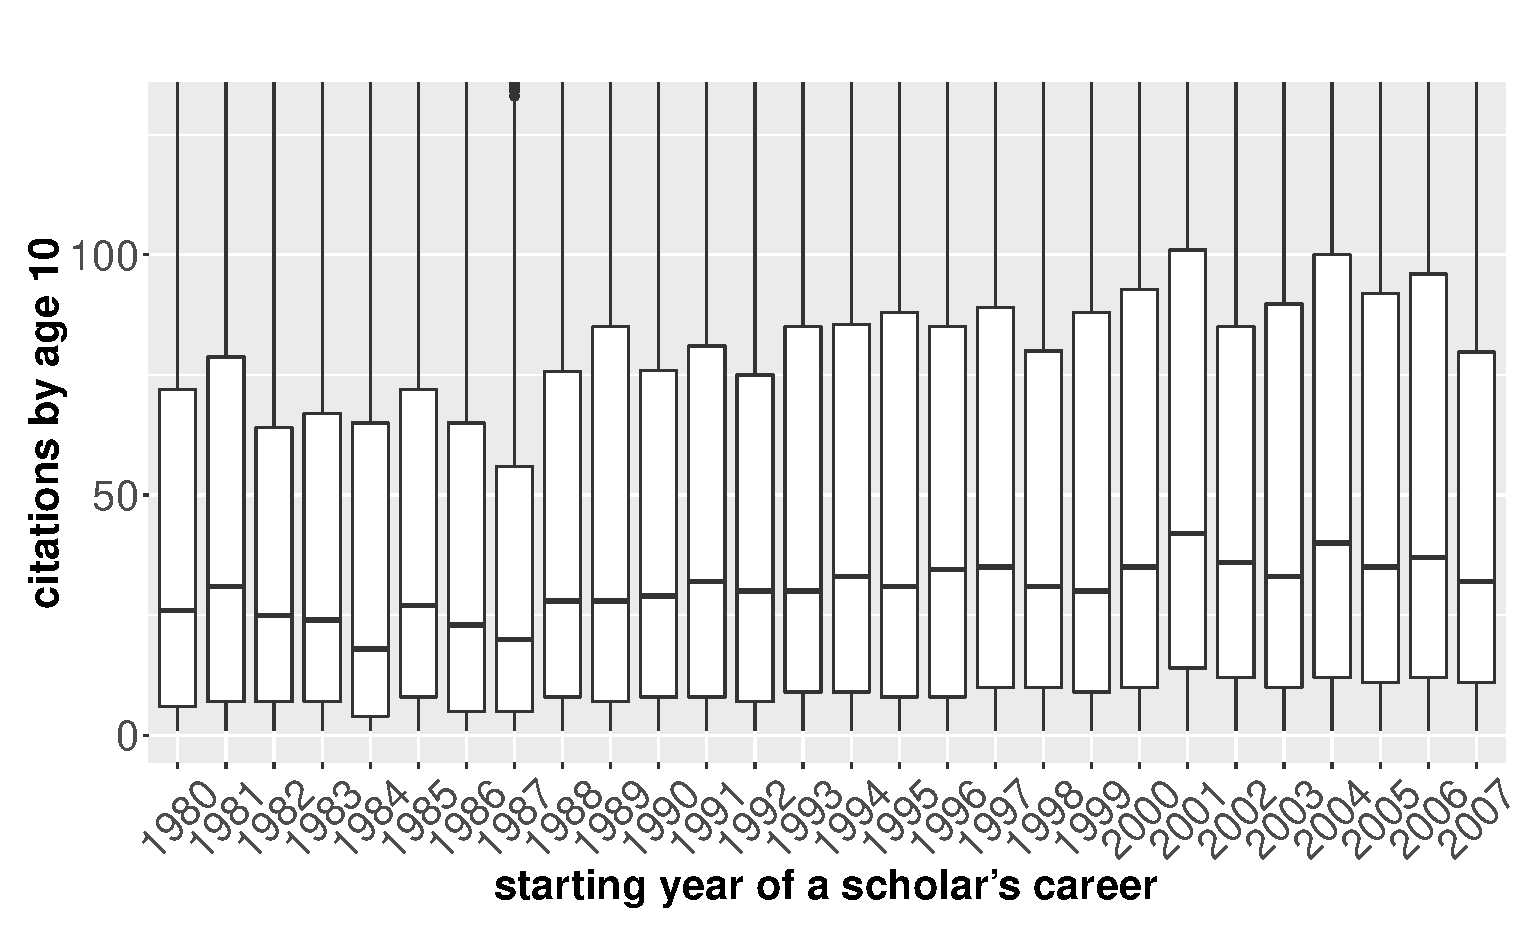
\includegraphics[width=\textwidth]{figures/exploratory/seniority_age10.eps}
         \caption{Total citations by age $10$ for papers published in $2007$}
     \end{subfigure}
    \caption{Seniority effect of scholars. The x-axis indicates starting years of careers of the corresponding authors. There's no evidence that senior scholars can attract more citations than junior scholars.}
    \label{fig:seniority}
\end{figure}

\begin{figure}[h!]
     \centering
     \begin{subfigure}[b]{0.48\textwidth}
         \centering
         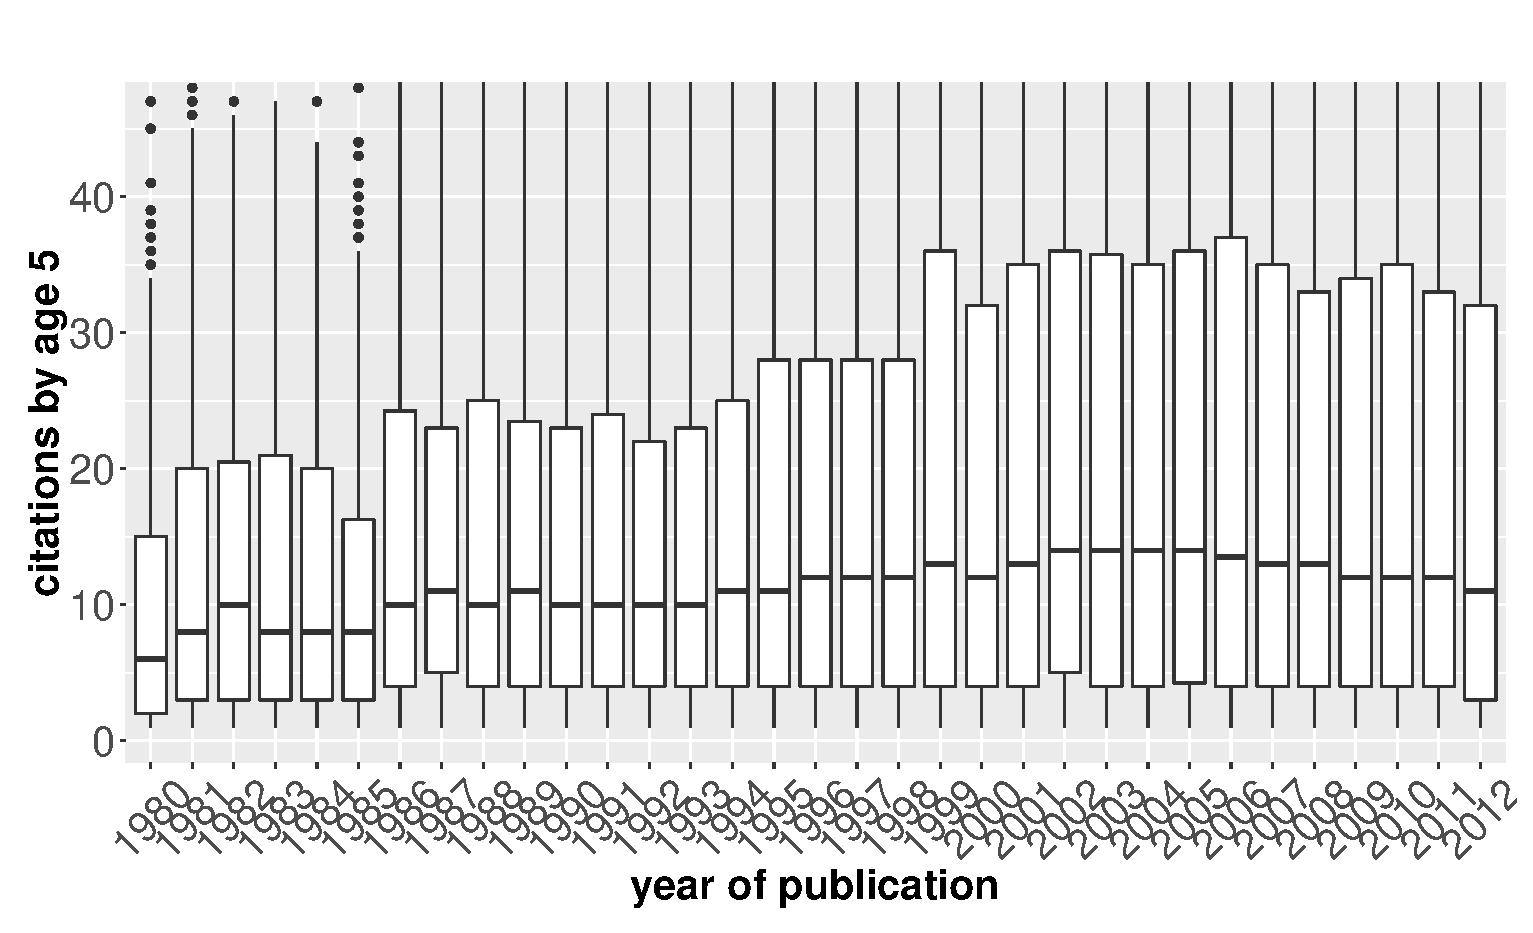
\includegraphics[width=\textwidth]{figures/exploratory/environment_age5.eps}
         \caption{Total citations by age $5$}
     \end{subfigure}
     \hfill
     \begin{subfigure}[b]{0.48\textwidth}
         \centering
         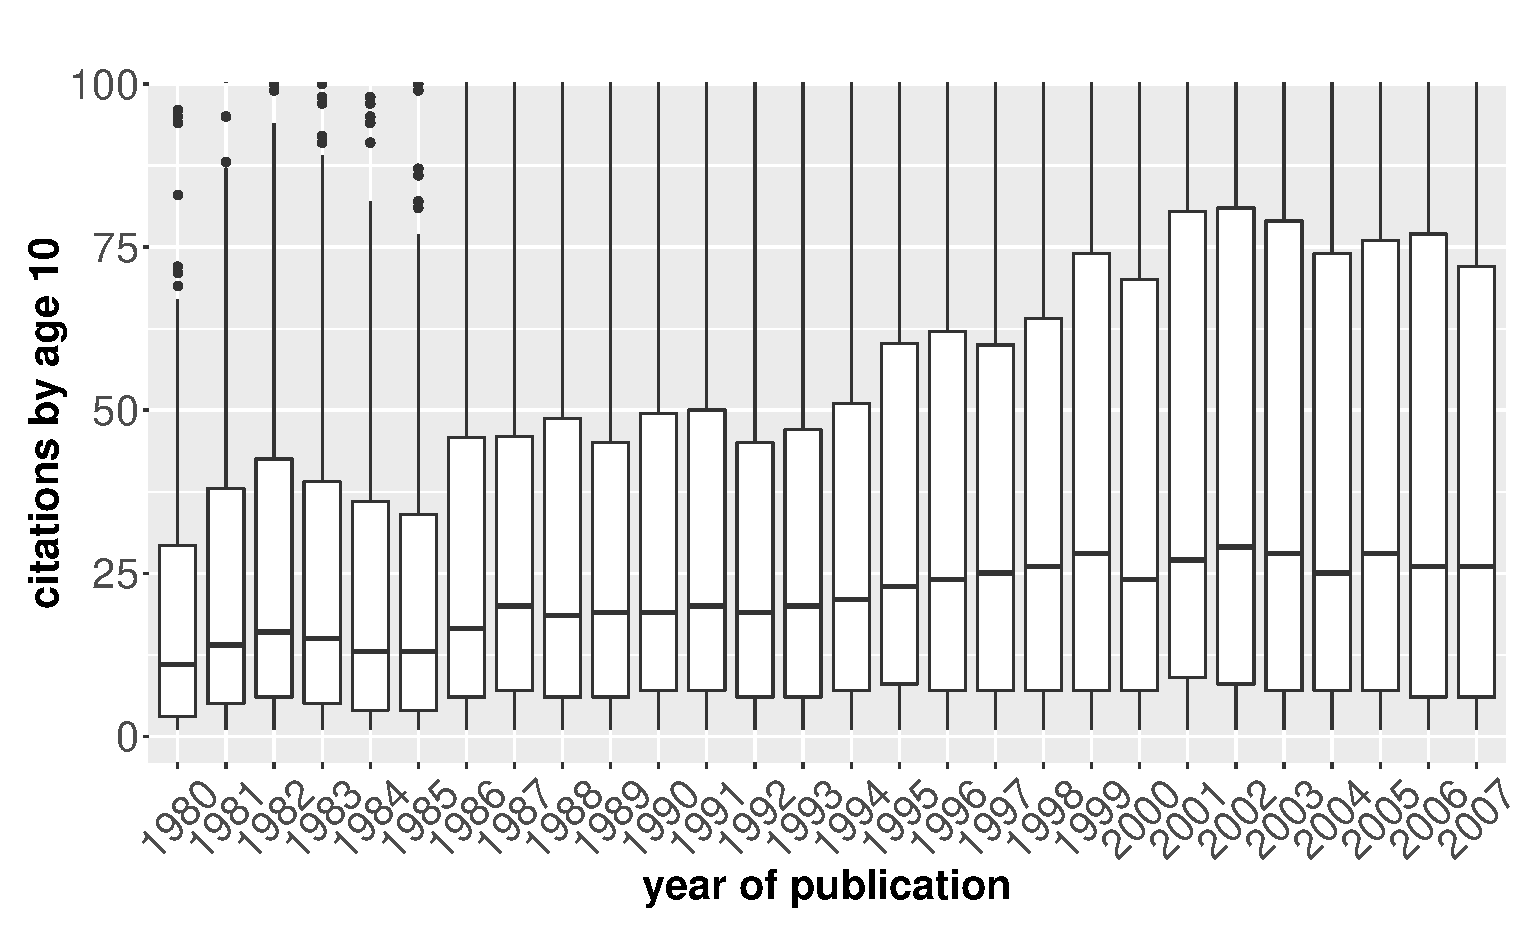
\includegraphics[width=\textwidth]{figures/exploratory/environment_age10.eps}
         \caption{Total citations by age $10$}
     \end{subfigure}
    \caption{Time effect. We consider the citations of the papers published by scholars who start their careers in year $1980$. The x-axis indicates the years of publication for their papers. We observe that more recent papers attract more citations than old papers.}
    \label{fig:environment}
\end{figure}

\begin{figure}[h!]
     \centering
     \begin{subfigure}[b]{0.48\textwidth}
         \centering
         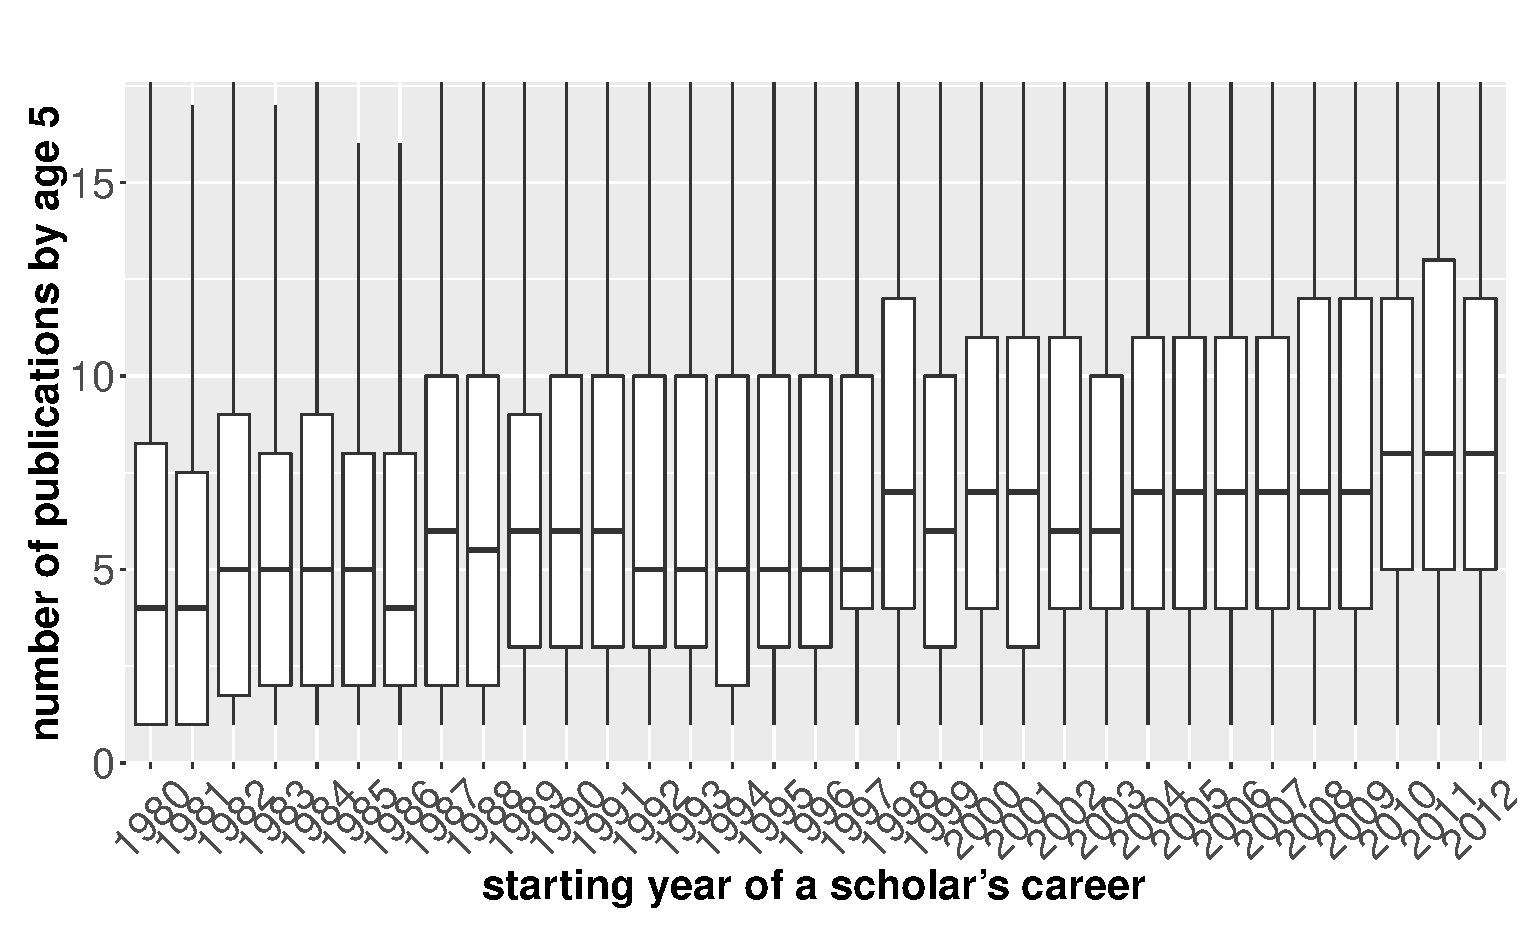
\includegraphics[width=\textwidth]{figures/exploratory/npub_age5.eps}
         \caption{Number of publications by age $5$}
     \end{subfigure}
     \hfill
     \begin{subfigure}[b]{0.48\textwidth}
         \centering
         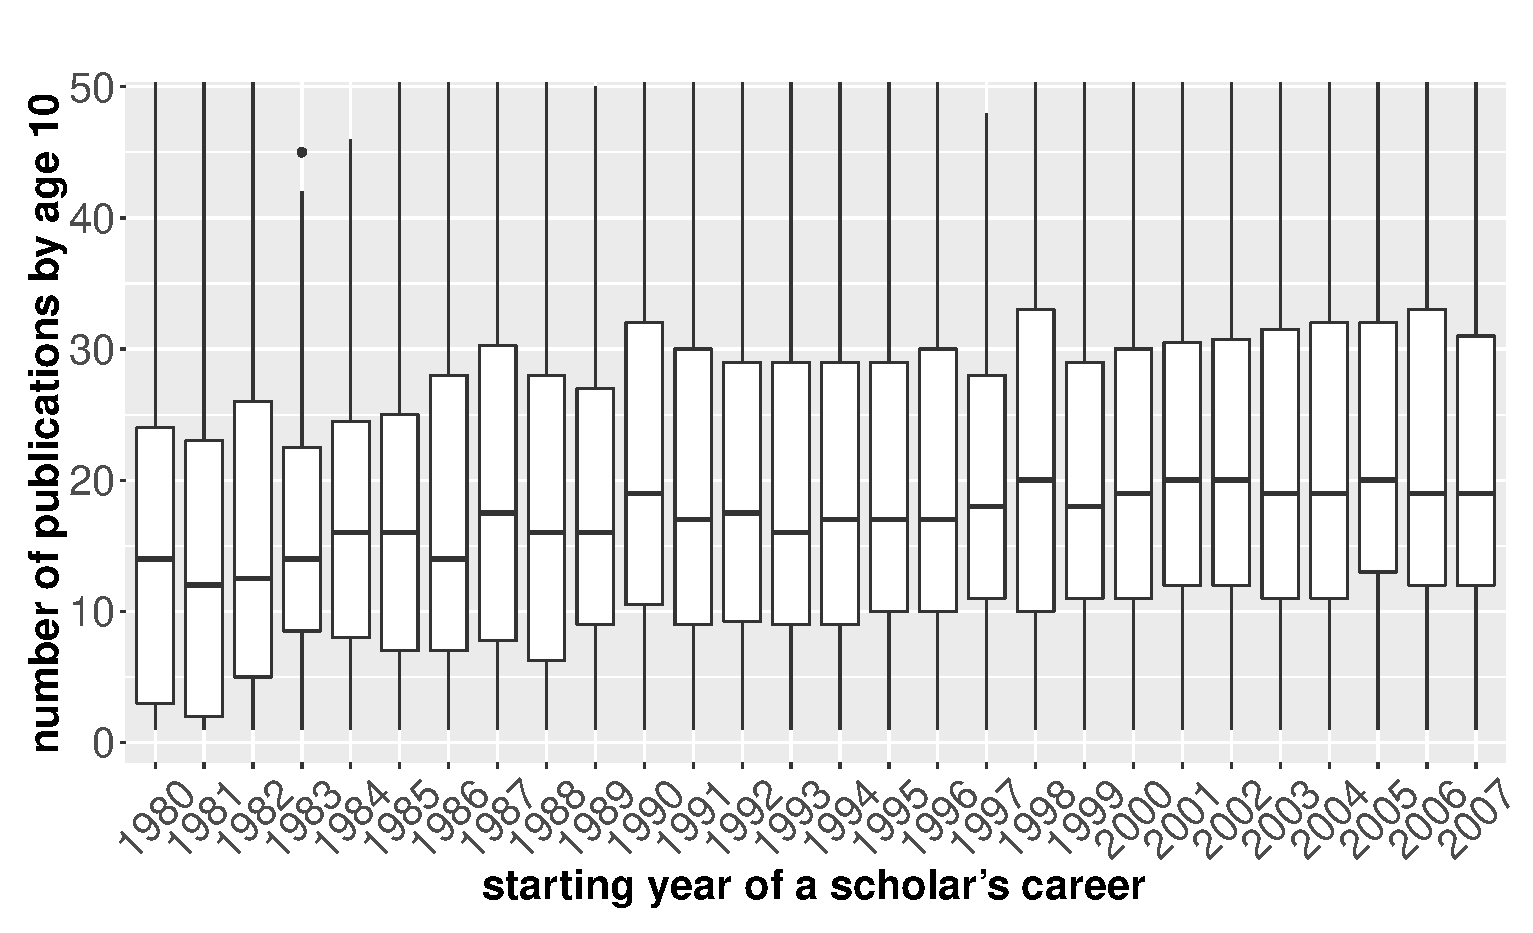
\includegraphics[width=\textwidth]{figures/exploratory/npub_age10.eps}
         \caption{Number of publications by age $10$}
     \end{subfigure}
    \caption{Number of publications. The x-axis indicates the starting years of careers of scholars. }
    \label{fig:npub}
\end{figure}


\begin{figure}[h!]
     \centering
     \begin{subfigure}[b]{0.48\textwidth}
         \centering
         \includegraphics[width=\textwidth]{figures/exploratory/rpc_age5.eps}
         \caption{rp.c$_{i5}$}
     \end{subfigure}
     \hfill
     \begin{subfigure}[b]{0.48\textwidth}
         \centering
         \includegraphics[width=\textwidth]{figures/exploratory/rpc_age10.eps}
         \caption{rp.c$_{i10}$}
     \end{subfigure}
     \hfill
      \begin{subfigure}[b]{0.48\textwidth}
         \centering
         \includegraphics[width=\textwidth]{figures/exploratory/rph_age5.eps}
         \caption{rp.h$_{i5}$}
     \end{subfigure}
     \hfill
     \begin{subfigure}[b]{0.48\textwidth}
         \centering
         \includegraphics[width=\textwidth]{figures/exploratory/rph_age10.eps}
         \caption{rp.h$_{i10}$}
     \end{subfigure}
      \hfill
      \begin{subfigure}[b]{0.48\textwidth}
         \centering
         \includegraphics[width=\textwidth]{figures/exploratory/rprp5new_age5.eps}
         \caption{rp.rp5$_{i5}$}
     \end{subfigure}
     \hfill
     \begin{subfigure}[b]{0.48\textwidth}
         \centering
         \includegraphics[width=\textwidth]{figures/exploratory/rprp5new_age10.eps}
         \caption{rp.rp5$_{i10}$}
     \end{subfigure}
    \caption{Different types of rank percentile indicators for scholars. rp.rp5 is stationary, while the other two are not.}
    \label{fig:compare_autrp}
\end{figure}

\fi

\end{refsection}



\end{document}
